%!TEX program = pdflatex
%!BIB program = biber

%% --------------------------------------------------------------------
%% thesis.tex -- MAIN FILE (the one that you compile with LaTeX)
%% --------------------------------------------------------------------
%% version 1.8.09.02.16 (beta)

%-----<<<<<<<<<<<< START >>>>>>>>>>>>-----
\documentclass[a4paper,12pt]{report}
\usepackage[a-2u]{pdfx}      		
\usepackage[cp1250]{inputenc}	%cp1250 for Czechoslovak characters, utf8
\usepackage{lmodern}
\usepackage[T1]{fontenc}
% \usepackage{fontenc}
% \usepackage{fontspec}
\usepackage{textcomp}

%-----<<< --------------------------------- >>>-----

%-----<<<<<<<<<<<< DEFINITIONS >>>>>>>>>>>>----- % for special characters of Czech/Slovak lang. use LaTeX commands only such as accute accent \'{o}, caron over the letter \v{s}, etc..
\def \BookName {DISSERTATION}
\def \Bookname {Three Essays on Financial Development}
\def \BooknameCZ {T\v{r}i eseje o rozvoji finan\v{c}n\'{i}ho sektoru} 
\def \AutorDP {Mgr. Jan Mare\v{s}}													
\def \AuthorDP {Mgr. Jan Mares} 			%here use just English characters!
\def \FirstNameDP {Jan} 				
\def \LastNameDP {Mare\v{s}} 							
\def \Email {janxmares@gmail.com}
\def \Year {2020}
\def \Place {Prague}
\def \Subject {Three Essays on Financial Development}
\def \Keywords {Finance, Growth, Wealth inequality, Income inequality, Bayesian Model Averaging}
\def \Klic {Finance, Ekonomick\'{y} r\r{u}st, Nerovnost bohatstv\'{i}, P\v{r}\'{i}jmov\'{a} nerovnost, Bayesi\'{a}nsk\'{y} model pr\r{u}m\v{e}rov\'{a}n\'{i}} 					
\def \JEL {\href{http://ideas.repec.org/j/C11.html}{C11},			%http://www.aeaweb.org/journal/elclasjn_hold.html
            \href{http://ideas.repec.org/j/D31.html}{D31},
            \href{http://ideas.repec.org/j/E21.html}{E21},
            \href{http://ideas.repec.org/j/G10.html}{G10},								%change the codes in the argument and also in the URL
            \href{http://ideas.repec.org/j/O40.html}{040}}	
\def \Thesisweb {}		%thesis webpage (leave empty if you use none)
\def \AcademicYear {2019/2020}
\def \Supervisor {prof.\ Roman Horv\'{a}th, Ph.D.}
% \def \StudyProgram {Economics and Finance}
\def \EmailSup {roman.horvath@gmail.com}
\def \CUNI {Charles University}
\def \FSS {Faculty of Social Sciences}
\def \IES {Institute of Economic Studies}
%-----<<< --------------------------------- >>>-----

%-----<<< METADATA >>>-----%filecontents must be in form of text, do not put definition reference like ``\AuthorDP'' inside
%\usepackage{filecontents}
%\begin{filecontents*}{Thesis.xmpdata}
%		\Author{Firstname Lastname} 
%		\Title{The Price Elasticity of Gasoline Demand: A Meta-Analysis}
%		\Keywords{keywordone, keywordtwo, keywordthree, keywordfour}
%		\Subject{Price Elasticity of Gasoline Demand}
%		\Publisher{Charles University} 
%\end{filecontents*} 

%-----<<<<<<<<<<<< STYLES >>>>>>>>>>>>-----      														
\usepackage{Styles/Head}
\usepackage{Styles/Mystyle}
%-----<<< --------------------------------- >>>-----

%-----<<<<<<<<<<<< BIBLIOGRAPHY with biblatex >>>>>>>>>>>>-----      														
\usepackage[style=apa]{biblatex}
\DeclareSourcemap{
  \maps[datatype=bibtex]{
    \map{ % set fields in .bib file to ignore
      \step[fieldset=issn, null]
      \step[fieldset=isbn, null]
      \step[fieldset=abstract, null]
      \step[fieldset=doi, null]
      \step[fieldset=url, null]
    }
  }
}
%
\addbibresource{Styles/literature.bib}	% bib file
%-----<<< --------------------------------- >>>-----

%-----<<<<<<<<<<<< DOCUMENT >>>>>>>>>>>>-----
\begin{document}
\frontmatter                   									%lowercase roman pagination for front matter
\clubpenalty 9999 															%not so many orphants
\widowpenalty 9999 															%not so many widows

%-----<<< HEAD >>>-----
\pagestyle{empty}                       				%no visible pagination here                    
\BookHead
%-----<<< ---- >>>-----
%-----<<< DECLARATION >>>-----
\vfill

\vglue 14cm

\section*{Declaration of Authorship}
The author hereby declares that he or she compiled this thesis independently, using only the listed resources and literature, and the thesis has not been used to obtain any other academic title.

\bigskip 

\noindent The author grants to Charles University permission to reproduce and to distribute copies of this thesis in whole or in part and agrees with the thesis being used for study and scientific purposes.
\vspace{0.5cm}

\begin{table}[!hbp]
\begin{tabular}{lr}
\hspace{-0.3cm} Prague, \today
\hspace{3cm}       
 \begin{tabular}{p{4.5cm}}
    \vspace{0.6cm} \\
     \hline \\ 
		\vspace{-0.7cm} \hspace{0.6cm} \AuthorDP
 \end{tabular}

\end{tabular}
\end{table}
        					%input file
\clearpage
%-----<<< ----------- >>>-----


%-----<<< ABSTRACT >>>-----
\phantomsection													 				%bookmark anchor
\pdfbookmark[0]{Abstract}{abst}        	 				%add bookmark
\section*{Abstract}

The abstract should concisely summarize the
contents of a thesis. Since potential readers should be able to
make their decision on the personal relevance based on the abstract,
the abstract should clearly tell the reader what information
he can expect to find in the thesis. The most essential issue
is the problem statement and the actual contribution of described
work. The authors should always keep in mind that the
abstract is the most frequently read part of a thesis. It should
contain at least 70 and at most 120 words (200 when you are writing a thesis).
Do not cite anyone in the abstract.

\bigskip

\begin{tabular}{lp{8.6cm}}
		\textbf{JEL Classification} & \JEL \\
		\textbf{Keywords} & \Keywords \\
 		& \\
		\textbf{Title} & \Bookname \\
 		\textbf{Author's e-mail} & \texttt{\href{mailto:\Email}{\Email}}\\
		\textbf{Supervisor's e-mail} & \texttt{\href{mailto:\EmailSup}{\EmailSup}}\\
\end{tabular}

\bigskip

\section*{Abstrakt}\label{abstract}

Nutnou sou��st� pr�ce je anotace, kter� shrnuje v�znam pr�ce a v�sledky v n� dosa�en�. Anotace pr�ce by nem�la b�t del�� ne� 200 slov a p�e se v jazyce pr�ce (tj.\ �esky, slovensky �i anglicky) a v p�ekladu (tj.\ u anglicky psan� pr�ce �esky �i slovensky, u �esky �i slovensky psan� pr�ce anglicky). Anotace pr�ce by nem�la b�t del�� ne� 200 slov a p�e se v jazyce pr�ce (tj. �esky, slovensky �i anglicky) a v p�ekladu (tj.\ u anglicky psan� pr�ce �esky �i slovensky, u �esky �i slovensky psan� pr�ce anglicky). V abstraktu by se nem�lo citovat.

\bigskip

\begin{tabular}{lp{7.7cm}}
		\textbf{Klasifikace JEL} & \JEL \\
		\textbf{Kl��ov� slova} & \Klic \\
 		& \\
		\textbf{N�zev pr�ce} & \BooknameCZ \\
 		\textbf{E-mail autora} & \texttt{\href{mailto:\Email}{\Email}}\\
		\textbf{E-mail vedouc�ho pr�ce} & \texttt{\href{mailto:\EmailSup}{\EmailSup}}\\
\end{tabular}

       					%input file
\clearpage
%-----<<< -------- >>>-----

%-----<<< ACKNOWLEDGMENTS >>>-----
\section*{Thank you}
Roman, I am very grateful for your patient encouragement and guidance throughout my Ph.D. studies. Your professionalism, work ethics, and life-view have been very inspirational to me.

Anna, thank you for helping me through the challenges in life and respectfully giving me the opportunity to pursue this and other endeavours alongside you.

To the rest of my family, thank you for your ever-present support.

\bigskip

\section*{Acknowledgments}
Research presented in Chapter \ref{ch3} of this dissertation is part of a project that has received funding from the European Union's Horizon 2020 research and innovation programme under the Marie Sklodowska-Curie grant agreement No.\ 681228. The author also acknowledges the support from Grant Agency of Charles University No. 768217.

\vfill

\noindent Typeset in \LaTeX  using the \href{https://is.cuni.cz/studium/eng/predmety/index.php?do=predmet&kod=JEM001}{IES Thesis Template}. 

\bigskip

\noindent \textbf{Bibliographic Record} \\
\LastNameDP, \FirstNameDP: \emph{\Bookname}. \BookName. \CUNI, \FSS, \IES, \Place. \Year, pages \ref*{TotPages}. Supervisor: \Supervisor


      						%input file
\clearpage
%-----<<< --------------- >>>-----

%-----<<< TABLE OF CONTENTS >>>-----
\pagestyle{fancy} 											 				%headers style
\fancyhead[LO]{\sffamily Contents}			 				%headers in sans serif and not in uppercase
\phantomsection													 				%bookmark anchor
\pdfbookmark[0]{Contents}{toc}        	 				%add bookmark
\tableofcontents
\label{toc}
\clearpage
%-----<<< ----------------- >>>-----

%-----<<< LIST OF TABLES >>>-----
\fancyhead[LO]{\sffamily List of Tables}				%headers in sans serif and not in uppercase
\phantomsection																	%bookmark anchor
\addcontentsline{toc}{chapter}{List of Tables}	%add LofT to the Table of Contents
\listoftables
\clearpage
%-----<<< --------------- >>>-----

%-----<<< LIST OF FIGURES >>>-----  
\fancyhead[LO]{\sffamily List of Figures}
\phantomsection																	%bookmark anchor
\addcontentsline{toc}{chapter}{List of Figures}	%add LofF to the Table of Contents
\listoffigures
\clearpage
%-----<<< ---------------- >>>-----

%-----<<< ACRONYMS >>>-----   
\fancyhead[LO]{\sffamily Acronyms}
\phantomsection																	%bookmark anchor
\addcontentsline{toc}{chapter}{Acronyms}				%add Acronyms to the Table of Contents
\chapter*{Acronyms}

\begin{acronym}[IVBMA]
{\setlength{\baselineskip}%
{0.67\baselineskip}
\acro{BIC}{Bayesian Information Criterion}
\acro{BIS}{Bank for International Settlements}
\acro{BMA}{Bayesian Model Averaging}
\acro{BRIC}{Bayesian Risk Inflation Criterion}
\acro{CBF}{Conditional Bayes Factor}
\acrodefplural{CBF}[CBFs]{Conditional Bayes Factors}
\acro{CSWD}{Credit Suisse Wealth Databook}
\acro{DINA}{Distributional National Accounts}
\acro{EFW}{Economic Freedom of the World}
\acro{FDI}{Foreign Direct Investment}
\acrodefplural{FDI}[FDIs]{Foreign Direct Investments}
\acro{GDP}{Gross Domestic Product}
\acro{GFDD}{Global Financial Development Database}
\acro{HBS}{Household Balance Sheet}
\acro{IID}{Independent Identically Distributed}
\acro{IVBMA}{Instrumental Variable Bayesian Model Averaging}
\acro{LIS}{Luxembourg Income Study}
\acro{MCMC}{Markov-chain Monte Carlo}
\acro{ML}{Marginal Likelihood}
\acro{OECD}{Organisation for Co-operation and Development}
\acro{OLS}{Ordinary Least Squares}
\acro{PIP}{Posterior Inclusion Probability}
\acrodefplural{PIP}[PIPs]{Posterior Inclusion Probabilities}
\acro{PMP}{Posterior Model Probability}
\acrodefplural{PMP}[PMPs]{Posterior Model Probabilities}
\acro{PWT}{Penn World Table}
\acro{SWIID}{Standardized World Income Inequality Database}
\acro{UIP}{Unit Information Prior}
\acro{UK}{United Kingdom}
\acro{US}{United States}
\acro{WALS}{Weighted-average Least Squares}
\acro{WB}{World Bank}
\acro{WID}{World Inequality Database}
\acro{WIID}{World Income Inequality Database}

\par}
\end{acronym}									%List of Acronyms
\clearpage
%-----<<< ---------------- >>>-----

%-----<<< THESIS PROPOSAL >>>----- 
% \fancyhead[LO]{\sffamily Master's Thesis Proposal}
% \phantomsection																	%bookmark anchor
% \addcontentsline{toc}{chapter}{Thesis Proposal}	%add Proposal to the Table of Contents
% \chapter*{Master's Thesis Proposal}

\begin{tabular}{lp{10.1cm}}
		\hline
		\textbf{Author} &\href{mailto:\Email}{\AutorDP}\\
		\textbf{Supervisor} &\href{mailto:\EmailSup}{\Supervisor}\\
		\textbf{Proposed topic} &\Bookname\\
		\hline
\end{tabular}

\bigskip

\small
\paragraph{Motivation}

For the purposes of government policy concerning energy security, optimal taxation, and climate change, precise estimates of the price elasticity of gasoline demand are of principal importance. For example, if gasoline demand is highly price-inelastic, taxes will be ineffective in reducing gasoline consumption and the corresponding emissions of greenhouse gases. During the last 30 years the topic has attracted a lot of attention of economists who produced a plethora of empirical estimates of both short- and long-run price elasticities. Yet the estimates vary broadly.

A systematic method how to make use of all this work is to collect these numerous estimates and summarize them quantitatively. The method is called meta-analysis (Stanley, 2001) and has long been used in economics following the seminal contribution by Stanley and Jarrell (1989). Recent applications of meta-analysis in economics include, among others, Card et al. (2010) on the evaluation of active labor market policy, Havranek (2010) on the trade effect of currency unions, and Horvathova (2010) on the impact of environmental performance on corporate financial performance.

Two international meta-analyses of the elasticity of gasoline demand have been conducted (Brons et al., 2008; Espey, 1998). These meta-analyses study carefully the causes of heterogeneity observed in the literature. The average short- and long-run elasticities found by these meta-analyses were -0.26 and -0.58 (Espey, 1998) and
-0.34 and -0.84 (Brons et al., 2008). None of the meta-analyses, however, corrected the estimates for publication bias. It is well-known that publication selection can seriously bias the estimates of price elasticities because positive estimates are usually inconsistent with theory: for instance, Stanley (2005) documents how the price elasticity of water demand is exaggerated fourfold because of publication bias.

\paragraph{Hypotheses}
\begin{enumerate}
		\item[] Hypothesis \#1: The literature estimating gasoline demand elasticities is affected by publication bias.
		\item[] Hypothesis \#2: The publication bias exaggerates the mean reported elasticity.
		\item[] Hypothesis \#3: The extent of publication bias decreases in time.
\end{enumerate}

\paragraph{Methodology}

The first step of meta-analysis is the collection of primary studies. I will examine all studies used by the most recent meta-analysis (Brons et al., 2008), but because the sample used by Brons et al. (2008) ends in 1999, I will additionally search the EconLit and Scopus databases for new studies published. To be able to use modern meta-analysis methods and correct for publication bias, I need the standard error of each estimate of elasticity; therefore I will have to exclude studies that do not report standard errors (or any other statistics from which standard errors could be computed). Concerning the definition of short- and long-term elasticity estimates, I will follow the approach described in the first meta-analysis on this topic, Espey (1998).

In the absence of publication bias the estimates of elasticities are randomly distributed  around  the  true  mean  elasticity. Nevertheless, if some estimates end in the ``file drawer'' (Rosenthal, 1979) because they are insignificant or have a positive sign, the reported estimates will be correlated with their standard errors (Ashenfelter et al., 1999; Card and Krueger, 1995). For example, if a statistically significant effect is required, an author who has few observations may run a specification search until the estimate becomes large enough to offset the high standard errors. In this specification the regression coefficient corresponding to the standard error measures the magnitude of publication bias and the intercept measures the magnitude of the elasticity corrected for publication bias (thus, the specification directly addresses hypotheses 1 and 2). Because such a regression is likely heteroscedastic (the explanatory variable is a sample estimate of the standard deviation of the response variable), in practice it is usually estimated by weighted least squares with the inverse of standard errors (precision) taken as weights.

In meta-analysis I have to take into consideration that estimates coming from one study are likely to be dependent. A common way how to cope with this problem is to employ the mixed-effects multilevel model (Doucouliagos and Stanley, 2009), which allows for unobserved between-study heterogeneity. Between-study heterogeneity is likely to be substantial since in our case the primary studies use data from different countries. I will specify the model following Havranek and Irsova (2011): the overall error term now breaks down into study-level random effects and estimate-level disturbances. To address hypothesis 3 I will add an interaction term between the year of publication of the study and the reported standard error. I expect that the magnitude of publication bias to decrease in time, which would be in line with the economics-research-cycle hypothesis (Goldfarb, 1995; Stanley et al., 2008).

\paragraph{Expected Contribution}

I will conduct a quantitative survey of journal articles estimating the price elasticity of gasoline demand. In contrast to previous meta-analyses on this topic, I will take into account publication selection bias using the mixed-effects multilevel meta-regression. Publication bias in this area is expected to be strong; when I correct for the bias, I expect to obtain estimates of short- and long-run elasticities that are much smaller than the results of the previously published meta-analyses and also to the simple mean of all estimates in my sample of literature. The estimates can be directly used in fiscal modeling (calculating the optimal tax on gasoline) and climate change policy (for example, the computation of the social cost of carbon emissions).

\paragraph{Outline}
\begin{enumerate}
	\item Motivation: there are meta-analyses on the price elasticity of gasoline demand, but they do not correct their estimates for publication bias. Publication bias has been shown to distort most areas of empirical economics, so there is a good chance it will be important here as well.
	\item Studies on gasoline demand: I will briefly describe how people estimate the price elasticity of gasoline demand.
	\item Data: I will explain how I will collect estimates from studies estimating the elasticity.
	\item Methods: I will explain modern meta-analysis methods, including the funnel asymmetry test, precision effect test, and multilevel variants of these regressions.
	\item Results: I will discuss my baseline regressions and robustness checks.
	\item Concluding remarks: I will summarize my findings and their implications for policy and future research.
\end{enumerate}


\paragraph{Core bibliography}


\begin{enumerate}
\item[]Ashenfelter, O., Harmon, C., Oosterbeek, H., 1999. A review of estimates of the schooling/earnings relationship, with tests for publication bias. Labour Econ. 6 (4), 453-470.
\item[]Brons, M., Nijkamp, P., Pels, E., Rietveld, P., 2008. A meta-analysis of the price elasticity of gasoline demand. A SUR approach. Energy Econ. 30 (5), 2105-2122.
\item[]Card, D., Kluve, J., Weber, A., 2010. Active labour market policy evaluations: a meta-analysis. Econ. J. 120 (548), F452-F477.
\item[]Card, D., Krueger, A.B., 1995. Time-series minimum-wage studies: a meta-analysis. Am. Econ. Rev. 85 (2), 238-243.
\item[]Doucouliagos, H., Stanley, T.D., 2009. Publication selection bias in minimum-wage research? A meta-regression analysis. Br. J. Ind. Relat. 47 (2), 406-428.
\item[]Espey, M., 1998. Gasoline demand revisited: an international meta-analysis of elasticities. Energy Econ. 20 (3), 273-295.
\item[]Goldfarb, R.S., 1995. The economist-as-audience needs a methodology of plausible inference. J. Econ. Methodol. 2 (2), 201-222.
\item[]Havranek, T., 2010. Rose effect and the Euro: is the magic gone? Rev. World Econ. 146 (2), 241-261.
\item[]Havranek, T., Irsova, Z., 2011. Estimating Vertical Spillovers from FDI: Why Results Vary and What the True Effect Is. J. Int. Econ. 85 (2), 234-244.
\item[]Horvathova, E., 2010. Does environmental performance affect financial performance? A meta-analysis. Ecol. Econ. 70 (1), 52-59.
\item[]Rosenthal, R., 1979. The ``file drawer'' problem and tolerance for null results. Psychol. Bull. 86, 638-641.
\item[]Stanley, T.D., 2001. Wheat from Chaff: meta-analysis as quantitative literature review. J. Econ. Perspect. 15 (3), 131-150.
\item[]Stanley, T.D., 2005. Beyond publication bias. J. Econ. Surv. 19 (3), 309-345.
\item[]Stanley, T.D., Doucouliagos, H., Jarrell, S.B., 2008. Meta-regression analysis as the socioeconomics of economics research. J. Socio-Econ. 37 (1), 276-292.
\item[]Stanley, T.D., Jarrell, S.B., 1989. Meta-regression analysis: a quantitative method of literature surveys. J. Econ. Surv. 3 (2), 161-170.
\end{enumerate}


\vfill
\begin{table}[!hbp]
\begin{tabular}{lr}

 \begin{tabular}{p{3.5cm}}
     \hline \hspace{1cm} Author
 \end{tabular}
 
 \hspace{5.5cm}
 
 \begin{tabular}{p{3.5cm}}
     \hline \hspace{0.8cm} Supervisor
 \end{tabular}

 
 \end{tabular}
 \end{table}

\normalsize





									%Thesis proposal
% \clearpage
%-----<<< ---------------- >>>-----

%-----<<< MAIN MATTER >>>-----
\mainmatter                   									%start arabic pagination from 1
\autohdr
\begin{refsection}																				%automatic headers for main matter
\begin{refsection}
\chapter{Summary of the dissertation}
\label{ch1}
The Great Recession following the financial crisis of 2007-2008 reinvigorated the interest in the research of financial development and its impact on the real economy. Although it was a dominant view at the time that more finance is good for economic growth and equalizes opportunities, the crisis spurred questions about the non-linearities in finance effects and the existence of a \emph{healthy} threshold or the impact being conditional on the quality of institutions. New regulatory waves followed, focusing primarily on the stability of the individual financial intermediaries, but also on the overall systemic risk. 

The measurement of finance and financial development also came into question. Most of the researchers in the field relied on the size (depth) measurement of finance. These are, however, imperfect proxies of the functions ascribed to finance in the theoretical models \parencite{Levine2005}. When I was about to begin with my dissertation research, more detailed and sufficiently dense data on financial development were published by the World Bank. The information on the stability, efficiency, and access to financial intermediaries was not perfect. However, it indicated better alternatives to size in accurately capturing the channels through which finance affects the real economic phenomena. Together with the carefully adopted methodological approach in \ac{BMA}, which allows for a comparison of the relative importance of different financial proxies, it suggested a promising research path I decided to take. Given the relevance of the question at the time, economic growth was a straightforward first choice. The evolution of the debate on inequality in the aftermath of the financial crisis meant that the topics of wealth and income inequality naturally followed.

This thesis is a composition of three papers related to financial development and its consequences. When I mention financial development in this thesis, I refer to the ability of financial contracts, markets, and intermediaries to facilitate the screening of investment opportunities, the monitoring of investments, and the pooling, trading, and management of risk \parencite{demirgucc2009finance}. In selected chapters that follow, I often refer to the authorship as ``we,'' which reflects that some of the papers in this dissertation I wrote in collaboration with my supervisor professor Roman Horv\'{a}th and professor Iftekhar Hasan from Fordham University. I continue with the overviews of individual dissertation papers.

In \emph{Chapter 2 - What Type of Finance Matters for Growth? Bayesian Model Averaging Evidence}, we examine the effect of finance on long-term economic growth. We consider the size proxies jointly with indicators that assess the stability and efficiency of financial markets. In the paper, we address the inconclusive finance-growth nexus literature. While some claim financial development has positive effect on economic growth \parencite{AtjeJovanovich1993,KingLevine1993a,RajanZingales1998}, others hold that financial sector removes scarce resources from the economy \parencite{bolton2016cream,Tobin1984,axelson2015wall} and underpins greater exposure and vulnerability to crises, severely burdening the real sector in during periods of instability \parencite{Minsky1991,Stiglitz2000}. More recent papers also point towards decreasing returns to financial development and finance having negative consequences for growth when above a certain threshold \parencite{Arcandetal2012,LawSingh2014,RousseauWachtel2011}. 

We depart from the literature in two main features. First, we apply \ac{BMA} to solve the model uncertainty problem in growth regressions. The variety of theories of economic growth suggests a large number of determinants and results in considerable uncertainty about the ``true'' growth model. Using the \ac{BMA}, we can evaluate numerous regressors potentially relevant for economic growth and estimate their \ac{PIP}, the probability that they are relevant in explaining the dependent variable, additionally to the weighted mean and variance of the respective coefficients. \ac{BMA} essentially estimates varying combinations of explanatory variables and weights the coefficients using model fit. The methodology is solidly rooted in the statistical theory \parencite{Rafteryetal1997,Koopetal2007} and indirectly also helps us to tackle the potential of omitted variables bias, from which empirical work on finance and growth typically abstracts.

Second, we augment previous research by examining several financial development indicators simultaneously to account for the multidimensionality of financial systems. By jointly examining whether depth, stability, or efficiency is relevant for long-term growth, we re-examine and unify previous literature. The established functions of finance are difficult to operationalize in empirical research \parencite{Valickovaetal2014}, and there is no consensus on the measurement of financial development \parencite{KingLevine1993a}. The research dominantly uses depth of financial markets (credit / GDP ratio or stock market capitalization / GDP) as a measure of financial development. Employing the \ac{GFDD} and the indicators provided therein, we can approximate the function of the financial system in much more detail. We can discriminate between banking and stock markets as well as evaluate the relative importance of depth versus the alternative proxies of efficiency, stability, and access to finance. We may also reflect the claims that excessive financial development and financial instability are harmful to growth. Even thought he data coverage is still somewhat limited, we contribute to the literature by considering these additional dimensions of the financial sector in our regression analysis to provide a more exact picture of finance-growth nexus. We complement the data on financial development by the long-term growth dataset of \textcite{Fernandezetal2001}, which provides a rich set of possible explanatory variables capturing various economic, political, geographical, and institutional factors.

We find that bank efficiency is the only indicator of financial development, which is robustly related to economic growth and consistently shows very high \ac{PIP}. This result is consistent with the theoretical predictions sketched out by \textcite{Pagano1993}, who shows how the increased efficiency of financial intermediaries affects the channel between savings and investment and therefore leads to higher real growth. On the other hand, the relevance of the traditionally employed variables, such as credit to the private sector or stock market capitalization, is weaker. Additionally, we find no evidence for a non-linear effect of financial development. We subject our results to further robustness checks by focusing on different sample periods, employing alternative priors, and basic techniques to address endogeneity with no substantial effect on our conclusions. The policy relevance of the results is in highlighting the essential importance of measuring financial development to precisely describe its consequences. The regulatory changes in the financial industry should appreciate the relevance of financial intermediaries for long-term growth. We published the paper in \emph{The World Bank Economic Review}.

\emph{Chapter 3 - Finance and Wealth Inequality} extends the idea of distinct features of financial systems to the distribution of wealth. Wealth inequality markedly varies across countries \parencite{daviesetal2017}, and the interest of the paper is to uncover the drivers of these differences. Is it different degrees of redistribution, financial development, globalization, technological progress, education, economic development, or something else? Although measurement of wealth inequality advanced significantly \parencite{daviesetal2017,SaezZucman2016}, there is a lack of systematic evidence about the determinants of wealth inequality across countries.

The theoretical predictions of the wealth inequality drivers vary. Much discussed $r > g$ concept presented by \textcite{piketty2014} suggests there is a natural tendency towards increasing wealth inequality unless exogenously amended by redistribution or wars. The framework is criticized on many fronts, though \parencite{mankiw2015yes,blume2015capital,king2017literature}, and the cornerstone remains with distinct applications of dynamic quantitative models. The models\footnote{\textcite{DENARDI2017280} provide thorough overview of the model implementations.} critically rely on the saving motives of the individuals, and this leads us to the hypothesis of financial development being crucially relevant for wealth distribution. Another prediction about the financial system and wealth inequality arises from \textcite{pastor2016income} in which inequality is driven, among other things, by the ability of entrepreneurs to diversify their idiosyncratic risk. The empirical evidence is scarce as the research papers on inequality mostly turn to the distribution of income due to better data availability. Nonetheless, wealth is much more unevenly distributed than income \textcite{zucman2019,oecd2013crisis}, and income distribution is mostly used as an approximation of wealth distribution, while the latter would be more fitting given the theory \parencite{bagchi2015does}.

The lack of encompassing theoretical framework informs our methodological framework similarly as in the paper on finance and growth. We rely on \ac{BMA} in estimations to identify relevant determinants of wealth distribution. Moreover, we extend the analysis to address potential endogeneity more rigorously using the \ac{IVBMA}. \ac{IVBMA} mostly resembles the two-stage frequentist methods but accounts for model uncertainty in both stages. We further refresh and expand the set of regressors by constructing our original database, although conceptually, we similarly select the variables capturing economic, financial, institutional, regulatory, and political features of considered countries. We prefer the freedom about the choice of regressors over the comparability of our results with existing research as the paper is a pioneering work in this field. We also importantly update the indicators of financial development we employ. Rather than relying on single indicators capturing different dimensions of financial systems, we use complex indicators constructed from the \ac{GFDD} that describe the characteristics of financial systems by extracting information from multiple indicators in each dimension through principal component analysis.

We find that the set of key determinants is small, and financial development exerts a complex effect on wealth inequality. Whereas countries with deeper financial systems (large financial markets and financial institutions) exhibit greater wealth inequality, more efficient intermediation and access to finance are associated with less wealth inequality. Our results thus support the idea that sound financial systems may contribute to lower wealth inequality. Alongside financial development, we discover that education, redistribution, globalization, and political instability affect wealth distributions within countries. Better educated societies and more higher redistribution of income support the more egalitarian distribution of wealth, while globalization and political instability increase wealth inequality. The conclusions offer apparent policy alternatives of countermeasures to increasingly unequal distributions of wealth in inclusive and efficient financial systems alongside better education. The paper is forthcoming in the \emph{Journal of International Money and Finance}.

\emph{Chapter 4 - Finance and Inequality - panel BMA approach} is the last follow-up in the series of papers on financial development. The theoretical predictions and their ambiguity resemble the ones on wealth inequality and finance. In contrast with wealth, income inequality and the relation to finance are subject to research much more frequently, but with conflicting outcomes. A fundamental divide appears between financial development on the extensive and intensive margin. On the extensive margin, it might lead to more equal opportunities and outcomes as access to credit by previously disadvantaged groups allows human capital accumulation \parencite{braunetal2019,galormoav2004} and formation of new firms \parencite{banerjeenewman1990,evans1989estimated}. On the contrary, the intensive margin of financial development might inordinately benefit the rich incumbents who leverage financial services for their further benefit or to protect their existing rents \parencite{GreenwoodJovanovic1990,perotti2007investor}.

The paper re-examines the literature on finance and inequality by applying panel \ac{BMA} techniques, once more identify the main determinants of income distribution within countries. I contribute to existing research by showing that: 1) finance has a significant role in shaping the distribution of income, 2) the complexity of the relationship arises from the characteristics of financial systems, and 3) the effect varies across different parts of the income distribution. 

Reflecting the conclusions of the preceding chapter, efficiency and access to financial institutions appears to have the inequality reducing role. The depth of the financial system seemingly does not influence the overall measure of the income distribution (Gini index). However, when the focus is on the top income shares, the size of the financial markets and institutions coincide with a more concentrated distribution of income. Additionally, the paper also provides evidence on other popular hypotheses about increasing income inequality exploring the education \parencite{goldin2009race}, globalization \parencite{Jaumotte2013}, or technological progress \parencite{dabla2015causes}. Interestingly, the results associate globalization proxied by the trade openness with a higher concentration of income at the top of the distribution, but its relevance diminishes when the measure of inequality is the Gini index. A higher level of education tends to mitigate overall income inequality but remains irrelevant for the concentration of income among the top 1\%. For the technological progress, indirect evidence using the investment into research and development and intellectual property suggests a positive relationship, supporting the idea of increasing inequality due to advancement in technology.

% Relying on the global sample of countries. We identify many potentially relevant regressors hypothesized in the literature as potential drivers of wealth distribution. 

% Financial development debate following the crisis\dots

% \ac{BMA} useful in examining uncertain relationships\dots + what is it, well grounded in theory

% Roles of finance\dots + multidimensionality

\newpage
\printbibliography[heading=subbibliography]
\addcontentsline{toc}{section}{References}
\end{refsection}              %input field
\end{refsection}
% \begin{refsection}
\chapter{What Type of Finance Matters for Growth? Bayesian Model Averaging Evidence}
\label{ch2}
\blfootnote{This chapter was co-authored with Iftekhar Hasan and Roman Horv\'{a}th and published in the \emph{The World Bank Econonmic Review}. We thank Martin Feldkircher and seminar participants at 19th ICMAIF conference (Rethymno, Greece), 32nd International Symposium on Money, Banking and Finance (Nice, France) and 1st World Congress for Comparative Economics (Rome, Italy) for helpful comments. The views expressed here are those of the authors and not necessarily those of the Czech Ministry of Finance or Bank of Finland.}

\begin{quote}
\begin{center}\textbf{Abstract}\end{center}
	We examine the effect of finance on long-term economic growth using Bayesian model averaging to address model uncertainty in cross-country growth regressions. The literature largely focuses on financial indicators that assess the financial depth of banks and stock markets. We examine these indicators jointly with newly developed indicators that assess the stability and efficiency of financial markets. Once we subject the finance-growth regressions to model uncertainty, our results suggest that commonly used indicators of financial development are not robustly related to long-term growth. However, the findings from our global sample indicate that one newly developed indicator -- the efficiency of financial intermediaries -- is robustly related to long-term growth.     
	\end{quote}

\clearpage
\section{Introduction}
\label{ch2sec:intro}
Numerous studies investigate the effect of financial development on economic growth and predominantly conclude that there is a positive causal relationship between the two \parencite{KingLevine1993a, LevineZervos1998, AtjeJovanovich1993}. Nevertheless, some opposing views hold that the financial sector removes scarce resources from the rest of the economy \parencite{Tobin1984,Boltonetal2011} and encourages to greater exposure and vulnerability to crises, thus severely burdening the real sector during periods of instability \parencite{Kindelberger1978,Minsky1991,Stiglitz2000}. The effect of financial development on growth has recently drawn greater attention again because of the financial crisis that began in 2007-2008. Moreover, conclusions referring to diminishing and eventually negative returns from financial development have become increasingly common in the literature \parencite{Arcandetal2012,CecchettiKharroubi2012,LawSingh2014}. This highlights the importance of the financial sector for the functioning of the economy and has provoked extensive debate among policymakers. 

This paper evaluates the finance-growth nexus but differs from previous research in two main respects. First, it employs \ac{BMA} to overcome certain drawbacks of previous research approaches. \ac{BMA} is well grounded in statistical theory \parencite{Rafteryetal1997} and addresses the inherent regression model uncertainty, which is quite high in cross-country growth regressions \parencite{Fernandezetal2001, SalaiMartinetal2004, Durlaufetal2008}. The control variables in finance-growth regressions are often selected in a somewhat \textit{ad hoc} manner with reference to certain relevant theories while ignoring other relevant theories. 

\ac{BMA} essentially allows us to control for dozens of potentially relevant determinants of growth within a unifying framework. The variety of theories of economic growth has given rise to a large number of determinants and resulted in substantial uncertainty concerning the true growth model. In essence, the \ac{BMA} procedure estimates different combinations of explanatory variables and subsequently weights the coefficients using various measures of model fit. As a consequence, \ac{BMA} also conveniently limits concerns regarding omitted variable bias and its adverse consequences of inconsistently estimated coefficients, an issue that is typically abstracted from in the empirical work on finance and growth. \ac{BMA} is capable of evaluating numerous possible regressors and estimating their \ac{PIP}, i.e., the probability that they are relevant in explaining the dependent variable, in addition to the weighted mean and variance of their corresponding coefficients. While model averaging has become standard in the empirical growth literature \parencite{SalaiMartinetal2004, Durlaufetal2008}, it has not been applied to study the finance--growth nexus.  

Second, we differ from previous research by examining additional financial indicators to appreciate the multidimensionality of financial systems. Importantly, previous research, including recent studies implying that excessive financial development harms growth \parencite{Arcandetal2012,CecchettiKharroubi2012,LawSingh2014}, largely focuses on measures of the depth of financial development such as the credit to GDP ratio. We depart from existing literature in jointly examining whether the depth, stability or efficiency of financial markets (or all of them) is crucial for long-term growth. In doing so, we can unify and re-examine previous studies on the finance-growth nexus that show that a) financial development is conducive to growth, b) excessive financial development is not, and c) financial instability has negative consequences for growth.

The theoretical concepts regarding the functions of the financial industry are difficult to operationalize in empirical research, and there is no universal consensus regarding the measurement of financial development \parencite{KingLevine1993a}. Although measuring financial development is complex, researchers typically consider only those variables capturing financial depth, such as the credit to GDP ratio or stock market capitalization, to assess the degree of financial development. Financial indicators assessing the degree of financial access, financial stability or the efficiency of the financial industry have largely been ignored in cross-country studies due to data limitations. The newly developed \ac{GFDD} represents a significant improvement in this respect and provides a comprehensive set of financial indicators that reflect various functions and characteristics of the financial sector. In addition to financial depth, the \ac{GFDD} provides measures of the efficiency and stability of and access to financial markets. Although data availability remains somewhat limited, we extend the existing literature by including these additional dimensions of the financial sector in our regression analysis to more completely evaluate the effect of finance on growth. Specifically, the indicators we use represent the depth, stability, and efficiency of the banking sector and stock markets as defined by \textcite{Cihaketal2013}.\footnote{We did not include financial access indicators because of data unavailability. In our sample, the data on the proxy variable recommended for financial access by \textcite{Cihaketal2013}, bank accounts per 1,000 adults, are missing for 36 out of 60 countries. Including financial access in the analysis would therefore severely limit our cross-section of countries resulting in the non-negligible loss in the degrees of freedom. Nevertheless, we have examined alternative (less than ideal) financial access indicators from the \ac{GFDD} database (bank branches per 100,000 adults and ATMs per 100,000 adults), which are available for almost all countries in our sample. However, we fail to find these indicators to be decisive for the long-term growth.} In addition to the \ac{GFDD}, we employ the widely used dataset on the determinants of long-term growth developed by \textcite{Fernandezetal2001}, which encompasses over 40 explanatory variables capturing various economic, political, geographical, and institutional indicators. 

While it is commonly assumed that causality goes from financial development to economic growth, some scholars argue that a growing financial sector merely follows the increasing needs of the real economy or may be determined simultaneously with growth due to other factors. The quantitative survey of the finance and growth literature by \textcite{Valickovaetal2014}, for example, indicates that those studies ignoring endogeneity are more likely to report a stronger positive effect of financial development on growth. Although it is likely that a part of endogeneity in finance--growth nexus can be addressed by model averaging procedure (reducing omitted variable bias), we also examine the robustness of our results through specifications that employ the lagged explanatory variables. To the best of our knowledge, this is the first study to combine various characteristics of the financial sector, a rich dataset on growth, and an approach that addresses model uncertainty and endogeneity. As a result, our study addresses two main issues in finance--growth literature: 1) causality issues and 2) measurement of financial development.

Using data on real economic growth in 60 countries between 1960 and 2011, we find that bank efficiency is robustly related to long-term growth and exhibits very high \ac{PIP}. This finding corresponds to the predictions of theoretical model by \textcite{Pagano1993}, who shows that the efficiency of financial intermediaries is crucial for funneling savings to investment and therefore, for increasing real growth. The relevance of traditional variables, such as credit provided to the private sector or stock market capitalization, is weaker. In addition, we also fail to find a non-linear effect of financial development on growth.  Our results are robust to a series of checks such as employing a different sample period, different parameter priors or addressing endogeneity. Therefore, our results highlight that the approach to measuring financial development is crucial for the estimated effect of finance on growth. Our policy implication is that those managing the current worldwide wave of regulatory changes in the financial industry should not underestimate the importance of the efficiency of financial intermediaries for long-term growth.

This paper is structured as follows. Section \ref{ch2sec:litsurvey} provides a literature review on finance and growth. Section \ref{ch2sec:data} presents the data. We describe Bayesian model averaging in section 4. We provide the regression results in section 5. The conclusions are presented in section 6. An appendix with additional results follows. 
%
%
% 
%
%
\section{Empirical Literature on Finance and Growth}
\label{ch2sec:litsurvey}

We briefly survey the empirical literature on the effect of financial development on growth. In addition, we discuss certain issues regarding the measurement of financial development. We refer readers to \textcite{Levine2005}, \textcite{Ang2008} and \textcite{Valickovaetal2014} for more comprehensive surveys of this literature.\footnote{There is also literature on the determinants of financial development, see \textcite{Ang2013}, and \textcite{angkumar}.}

\subsection{Empirical Evidence}

Focusing on the period between 1960 and 1989, \textcite{KingLevine1993a} show how the initial levels of various financial indicators, such as the liabilities to the financial sector, bank ratios, credit to nonfinancial private sector/total domestic credit, and credit to the private sector to GDP, explain the real growth of GDP per capita, capital accumulation, and efficiency of capital utilization in the following period. \textcite{AtjeJovanovich1993} examine the stock market's effects on economic growth and find that more active stock markets induce growth. The conclusion regarding stock market activity is subsequently confirmed by \textcite{LevineZervos1998}. In addition to providing evidence on stock market effects, \textcite{LevineZervos1998} simultaneously control for banking sector development by including credit to the private sector. Interestingly, both the banking sector and stock markets are significant in fostering growth. This leads the authors to conclude that each of the sectors has a different function in the economy and a different financial function. Furthermore, they add that the mere size of the stock market as measured by total capitalization is irrelevant to growth and that the relevant factor is the activity of the stock market. Nevertheless, this link may be an outcome of an unobserved third factor that stimulates both trading activity and economic growth. For instance, information regarding new technology may spur trading activity due to conflicting opinions on the future benefits of the innovation. The subsequent economic growth is a result of technological advancement rather than greater trading volumes \parencite{Levine2005}. This is one of the reasons why we apply the \ac{BMA}, which is designed to address these issues.

\textcite{RajanZingales1998} initiate the research on the finance-growth nexus using industry-level data. They show that more developed financial markets decrease firms' cost of external capital. They also find evidence that industries that are relatively more dependent on external finance grow faster in countries with better developed financial intermediaries. Building on this methodology, \textcite{ClaessensLaeven2005} arrive at a similar conclusion using measures of bank competitiveness. They find that more competitive banking systems benefit financially dependent industries. Next, \textcite{Becketal2005} show that industries typically composed of small firms enjoy relatively superior growth rates in countries with developed financial sectors. This is consistent with theory positing that financial development is a crucial factor in alleviating financial constraints. Also, \textcite{Hasanetal2009} examine the effect of financial development on regional growth in Europe and find that the efficiency of financial intermediaries (measured by bank efficiency) is substantially more important for growth than financial depth (measured by outstanding credit). \textcite{Bergeretal2004} also provide international evidence on the importance of bank efficiency for growth. Similarly, using German data, \textcite{KoetterWedow2010} find that bank efficiency is positively related to growth. \textcite{JayaratneStrahan1996} report that the relaxation of bank branch restrictions in the United States improves growth. Interestingly, they find that the relaxation of restrictions does not increase the volume of bank lending but improves loan quality. In addition, \textcite{CetorelliStraha2006} extensively examine the mechanism how financial development affect growth and find that more competition among local U.S. banks improves firms' performance. 

Panel and time-series analyses predominantly claim that the relationship goes from financial development to growth rather than in the reverse direction, essentially moderating endogeneity concerns.  \textcite{ChristopoulosTsionas2004}, \textcite{Finketal2003} and \textcite{PeiaRoszbach2015} observe positive long-run growth effects of financial development using cointegration techniques. \textcite{ChristopoulosTsionas2004} argue in favor of long-run causality from financial development to growth and dismisses the backward channel. \textcite{Finketal2003} is one of the few papers investigating the relationship by considering private bond markets. \textcite{PeiaRoszbach2015} investigate the causality of the finance-growth relationship and demonstrate that the causality depends on the measurement employed and the level of financial development. Recently, \textcite{Thumrongvitetal2013} revisit the question and compare the impact of bond markets while also accounting for the role of the banking sector. They report that the importance of bank credit in determining growth declines as alternative debt financing options become increasingly available. Although studies positing "finance-lead" growth prevail, there are opposing views that stress finance's irrelevance in this respect. \textcite{Garretsenetal2004}, for example, document that the causal link reported by \textcite{RajanZingales1998} disappears after accounting for societal and legal factors. It may be that the development of financial markets simply follows growth, reflecting the needs of a more developed economy. Ultimately, accounting for time- and country-specific effects does not entirely eliminate the caveats applicable to such analyses. Time coverage is often short, and utilizing more frequent observations, such as quarterly data, does not properly address hypotheses concerning the long-term nature of the relationship \parencite{Ang2008}. 

Researchers have devoted greater attention to the finance and growth literature following the economic crisis of 2007-2008. They raise questions regarding possible non-linearities in the relationship between finance and growth, specifically, whether excessive financial development is harmful to growth. \textcite{RousseauWachtel2011} report that a positive correlation between the development of the financial sector and economic growth is typical for the period before 1990. The effect diminishes when subsequent years are considered. Additional studies report evidence of an inverted U-shaped relationship suggesting financial development is conducive to growth only up to a certain threshold. Thereafter, it acts as a drag on economic growth \parencite{CecchettiKharroubi2012,Arcandetal2012,LawSingh2014}. Some research advances explanations to justify these findings. One is the comparatively large amount of credit going to households in the later stages of financial development. These loans generally tend to be less productive than loans to enterprises \parencite{Becketal2012}. \textcite{CecchettiKharroubi2013} emphasize that a larger financial sector leads to lower total factor productivity through relatively larger benefits for high-collateral/low-productivity projects, primarily in construction. Other lines of reasoning rely on Tobin's early work discussing how finance lures talent from other sectors \parencite{Boltonetal2011,CecchettiKharroubi2012,Kneer2013}. \textcite{Yilmazkuday} shows that growth enhancing effect of finance depends on a number of factors such as price stability, economic development or trade openness. Overall, these recent empirical studies find that the growth-enhancing effects of financial development are not guaranteed and suggest that the relationship is more complex than originally thought.

\subsection{Measurement of Financial Development}
\textcite{Levine2005} argues that it is difficult to link empirical and theoretical research on finance and growth. Concepts such as information asymmetry, improved corporate governance, risk management, pooling savings, and easing exchange are in reality difficult to measure accurately.

The most common indicators of financial development address financial depth, primarily because of their widespread availability. Conventional variables used as proxies for the depth of the financial sector are total liquid liabilities of the financial sector, credit to the private sector, and various measures of monetary aggregates. The aforementioned variables depict the development of the banking sector, in stock market studies, broadly employed proxies include the ratio of total market capitalization to GDP, the total value traded to GDP (stock market activity ratio), and the total value traded to the total value of listed shares (turnover ratio).  

The extent to which these traditional measurements reflect the ability of financial intermediaries to serve the functions assigned to them in theory remains unclear. For instance, \textcite{Cihaketal2013} illustrate that private bond market capitalization represents a substantial share of the total securities market capitalization within a country. However, when addressing the question of depth, private bond markets are often ignored. In addition, total credit data do not include trade credit, where firms \textit{de facto} act as financial intermediaries \parencite{PetersenRajan1997}. In addition, \textcite{Levine2005} notes that this factor may be particularly important in countries with poor legal environments or overly regulated financial systems. Ultimately, there is no general consensus among researchers regarding the appropriate approach to measure financial development. Generally, studies consider several potential indicators to assess the robustness of their results, but these indicators are typically only proxies for the level of financial depth \parencite{Valickovaetal2014}.

Finally, some financial development measures such as the (rarely used) bank efficiency can be conceptually much more closely related to the theory \parencite{Pagano1993} than the traditional quantity measures such as the volume of credit granted. Bank efficiency is also less likely to be prone to causality issues because technical efficiency of banks respond less to the business cycle in comparison to, for example, the volume of credit \parencite{KoetterWedow2010}.

\section{Data}
\label{ch2sec:data}
We use the dataset from a seminal paper on long-term economic growth determinants and \ac{BMA} by \textcite{Fernandezetal2001}. The dataset contains 41 explanatory variables that might be important for growth in 72 countries. We update the dependent variable (average real economic growth per capita in 1960-2011). The regressors in the dataset comprise various measures of economic, political, geographic, demographic, social, and cultural factors. As many of these factors may be determined simultaneously with growth, the regressors typically come from 1960 or even before to alleviate endogeneity concerns. We describe this dataset in greater detail in the appendix.

To this dataset, we add selected financial indicators from the World Bank's \ac{GFDD} (September 2013 version), which collects information on various aspects of financial sectors around the globe. \textcite{Cihaketal2013} describe this dataset's content in detail and offer a 4x2 dimensional classification of financial indicators that reflects their utility in representing the depth, breadth, efficiency, and stability (4) of both the banking sector and the stock market (2). We choose to employ several indicators for which the database provides the richest data. Specifically, we select five different indicators representing various aspects of the financial system:

\begin{itemize}
	\item \textbf{Private sector credit to GDP:} domestic private credit to the real sector to GDP; a measure of the depth of the banking sector.
	\item \textbf{Stock market capitalization to GDP:} value of listed shares to GDP; a measure of the depth of stock markets.
	\item \textbf{Net interest margin:} accounting value of banks' net interest revenue as a share of average interest-bearing assets; a measure of the efficiency of the banking sector.
	\item \textbf{Stock market turnover ratio:} stock market value traded to total market capitalization; a measure of the efficiency of stock markets.
	\item \textbf{Bank Z-score:} return on banks' assets plus the ratio of banks' equity and assets, divided by the standard deviation of the return on assets $\left(\frac{ROA + \frac{equity}{assets}}{sd(ROA)}\right)$; a measure of the stability of the banking sector.
\end{itemize} 
%
The aforementioned dimensional distinction allows us to differentiate and compare the effects of the banking sector and the stock market on economic growth. In addition, unlike the previous literature, we simultaneously examine whether the depth, efficiency and stability of a financial system are important for growth. 

The time and cross-country coverage of financial variables varies. Private credit to the real sector is available for the majority of the countries in the dataset since 1960. However, the remaining variables are typically available only from the 1980s onward. We average the indicator values corresponding to a selected period (i.e., 1960-2011) and to their data availability. This is a standard procedure in estimating empirical long-term growth models, despite the risk of introducing endogeneity into the model and information loss introduced by averaging over extended time periods. The benefit of averaging is a focus on long-term trends while abstracting from short-term fluctuations. But in our robustness checks, we also use the initial values of financial indicators instead of their average. Given the data availability and the construction of the dataset, all the financial variables could be endogenous. We address endogeneity concerns through our \ac{BMA} approach using lagged variables. Table \ref{tab:descstat} presents descriptive statistics on the individual financial indicators. Overall, the combined dataset of \textcite{Fernandezetal2001} and private credit and new financial indicators leads to 68 and 60 observations, respectively.

\begin{table}[!ht]
	\caption{Descriptive statistics, financial indicators}
	\label{tab:descstat}
	\centering
	\begin{tabular}{lrrrrr}
		\toprule
		& Min & Max & Mean & Std.dev \\ 
		\midrule
		Net interest margin 		& 0.59 & 13.31 & 4.52 & 3.25 \\ 
		Bank Z-score				& -1.61 & 42.35 & 15.00 & 9.62 \\ 
		Private credit 			& 5.16 & 146.66 & 46.58 & 35.29 \\ 
		Market capitalization 	& 0.67 & 303.77 & 51.28 & 52.98 \\ 
		Market turnover 			& 0.96 & 197.50 & 48.22 & 47.13 \\ 
		\bottomrule
		
	\end{tabular}
\end{table}

\section{Bayesian Model Averaging}
\label{ch2sec:BMA}
To illustrate the application of BMA, we begin with a traditional linear model structure:
%
% OLS notation
\begin{equation}\label{ch2eq:OLS}
	y = \alpha + X\beta+ \varepsilon \qquad \varepsilon  \sim\ N(0, \sigma^{2}I)
\end{equation}
%
where $y$ is a dependent variable, $\alpha$ is a constant, $X$ is the matrix of explanatory variables, $\beta$ represents the corresponding coefficients, and $\varepsilon$ is a vector of normally distributed IID error terms with variance $\sigma^{2}$. In many applications, the list of potentially relevant regressors can be large. In the typical case in which the true regression model is unknown, its construction often begins by including all the variables in the model. However, this strategy is likely to yield imprecise estimates, as the large number of regressors inflates standard errors. Empirical research typically addresses this issue by sequentially eliminating the least significant explanatory variables on the basis of statistical tests to arrive at the single best model with all the irrelevant regressors omitted.

The process described above entails the risk of the researcher retaining an irrelevant variable or dropping an important variable. \textcite{Koop2003} emphasizes that the probability of making such mistakes increases rapidly with the number of sequences performed. The various iteration paths may also lead to different regression model specifications. In addition, even if we assume that this procedure identifies the 'best' model, it is rarely acceptable to present only the results from the single 'best' model and disregard the results of 'second-best' models. In summary, then, this model-selection approach ignores the model uncertainty that the researcher faces when she or he defines the model. \ac{BMA} allows the researcher to account for such uncertainty and presents a rigorous method for treating multiple models.

\ac{BMA} considers all possible combinations of $X$ from equation \ref{ch2eq:OLS} and takes a weighted average of the coefficients (see also the remarks on the \ac{MCMC} sampler below). The substructure of the model can be captured as follows:
%
% submodel structure
\begin{equation}\label{ch2eq:OLSsub}
	y = \alpha_{i} + X_{i}\beta_{i}+ \varepsilon \qquad \varepsilon  \sim\ N(0, \sigma^{2}I)
\end{equation}
%
Here, $X_{i}$ is a subset of $X$ and $\alpha_{i} $ and $ \beta_{i}$ are the corresponding coefficients. Assuming that the total number of possible explanatory variables is $K$, the total number of models is equal to $2^{K}$ and $i \in [1,2^{K}]$. 
%%
%%
%%

Researchers are interested in describing coefficients based on observed data. It follows from Bayes' rule that
%
% Bayes' rule with 'model' notation
\begin{equation}\label{ch2eq:BRmodel}
	p(\beta \vert y,X) = \frac{p(y,X\vert \beta)p(\beta)}{p(y,X)}
\end{equation}
where $p(\beta \vert y, X)$ is the posterior density, $p(y, X\vert \beta)$ is the marginal likelihood (ML), also known as the data generating process, $p(\beta)$ is the prior density, and $p(y,X)$ is the probability of the data. In the \ac{BMA}, we essentially compare numerous different models $M_{1},...,M_{i}$.  Assuming $K$ possible regressors as discussed above, we have $M_{1},...,M_{i}$, where $i \in [1,2^{K}]$. Given the Bayesian logic whereby we formally define the model using a likelihood function and a prior density, $M_{i}$ depends on the parameters $\beta_{i}$, and their posterior probability can be derived as follows:
\begin{equation}\label{ch2eq:BROM}
	p(\beta_{i} \vert M_{i},y,X) = \frac{p(y\vert \beta_{i},M_{i},X)p(\beta_{i}\vert M_{i})}{p(y \vert M_{i},X)}
\end{equation}
The following subsections describe the averaging principle of \ac{BMA} and individual components of equation \ref{ch2eq:BRmodel}.
%
%%
\subsection{Posterior Model Probability}
%%
%
The \ac{PMP} is fundamental to the \ac{BMA} framework, as it provides the weights for averaging model coefficients across submodels. \ac{PMP} also arises from Bayes' theorem:

\begin{equation}\label{ch2eq:PMPmain}
	p(M_{i} \vert y,X) = \frac{p(y\vert M_{i},X)p(M_{i})}{p(y \vert X)}
\end{equation}

where $p(y\vert M_{i},X)$ is the \ac{ML} of the model (i.e., the probability of the data given the model $M_{i}$), $p(M_{i})$ is the prior model probability, and $p(y\vert X)$ is the integrated likelihood. The term in the denominator is typically disregarded, as it is constant across all models under consideration. The PMP is then directly proportional to \ac{ML} and the prior probability. A popular practice is to set the prior probability $p(M_{i} \propto 1)$ to reflect the lack of knowledge regarding the true model.
% Proportionality of PMP
\begin{equation}
	p(M_{i}\vert y,X) \propto p(y\vert M_{i},X)p(M_{i})
\end{equation}
%
We discuss the calculation of \ac{ML} in detail in section \ref{ch2sec:ML}. The model prior needs to be elicited by the researcher and reflects the initial beliefs before inspecting the data. 
%
\subsection{Posterior Mean}
Point estimates of the model parameters are often the focus of research, and it is possible to derive them within the Bayesian framework. \textcite{Zeugner2011} and \textcite{MoralBenito2012} assert that the weighted posterior distribution of any statistic (most notably the $\beta$ coefficients) is obtained using the following:
%
%% Posterior distribution of the coefficients
\begin{equation}\label{ch2eq:parest}
	p(\beta \vert y, X) = \sum_{i=1}^{2^{K}} p(\beta_{i} \vert M_{i},y,X)p(M_{i} \vert y,X)
\end{equation}

where $p(M_{i} \vert y, X)$ is the \ac{PMP} of the corresponding model $M_{i}$ from equation \ref{ch2eq:PMPmain}. The point estimates can be acquired by taking expectations across the equation:

\begin{equation}\label{ch2eq:pointparest}
	E(\beta \vert y, X) = \sum_{i=1}^{2^{K}} E(\beta_{i} \vert M_{i},y,X)p(M_{i} \vert y,X)
\end{equation}

Here, $E(\beta \vert y, X)$ is the averaged coefficient and $E(\beta \vert M_{i},y,X)$ is the estimate of the $\beta_{i}$ coefficients from model $M_{i}$. The posterior distribution of the coefficients is dependent on the choice of the prior $g$. \textcite{Zeugner2011} expresses the expected value of the parameter in $M_{i}$ as follows:
\begin{equation}\label{ch2eq:postdist}
	E(\beta_{i} \vert y,X,g,M_{i}) = \frac{g}{1+g}\hat{\beta_{i}}
\end{equation}
with $\hat{\beta_{i}}$ representing the standard \ac{OLS} estimate.

\subsection{Posterior Variance}
\textcite{MoralBenito2012} presents a formula for variance corresponding to the expected values of coefficients derived in the previous section:
\begin{equation}\label{ch2eq:postvar}
	\begin{aligned}
		Var(\beta \vert y, X) &= \sum_{i=1}^{2^{K}} p(M_{i} \vert y,X)Var(\beta_{i} \vert M_{i},y,X) + \\ 
		&+\sum_{i=1}^{2^{K}}p(M_{i} \vert y,X){(E(\beta_{i}\vert M_{i},y,X)-E(\beta \vert y, X))}^{2}
	\end{aligned}
\end{equation}
The variance consists of the weighted average of variance estimates across different regression models $Var(\beta_{i} \vert M_{i},y,X)$ and the weighted variance across different models captured in the second component ${{E(\beta_{i}\vert  M_{i},y,X)}-{E(\beta \vert y,X))}}^{2}$. $E(\beta \vert y,X)$ is the posterior mean from equation \ref{ch2eq:pointparest}. As a consequence, this may result in uncertainty regarding the parameter estimates due to the substantial differences across models even if the estimates of individual models are highly precise. \textcite{Zeugner2011} shows how the value of the prior $g$ affects the posterior variance of the parameters:
%
% Posterior variance of betas
\begin{equation}\label{ch2eq:postvarZ}
	Cov(\beta_{i}\vert y,X,g,M_{i}) = \frac{(y-\bar{y})'(y-\bar{y})}{N-3} \frac{g}{1+g} \left( 1- \frac{g}{1+g}R_{i}^{2} \right) (X_{i}'X_{i})^{-1}
\end{equation}
where $\bar{y}$ is the mean of vector $y$, $N$ is the sample size and $R^{2}_{i}$ is the R-squared of model $i$.
%
%%
\subsection{Marginal Likelihood}\label{ch2sec:ML}
\ac{ML} can be calculated using equation \ref{ch2eq:BROM} for each $M_{i}$. We need to integrate both sides of the equation with respect to $\beta_{i}$, employ $\int_{\beta} p(\beta_{i}\vert M_{i},y,X) \, d\beta_{i}=1$, and rearrange to arrive at
%
% Marginal likelihood basic
\begin{equation}\label{ch2eq:ML}
	p(y \vert  M_{i},X) = \int_{\beta}{p(y \vert \beta_{i},M_{i},X)p(\beta_{i} \vert M_{i},X) \, d\beta_{i}}
\end{equation}
%%
The above equation illustrates the general textbook derivation, but the computation depends on the elicited priors. \textcite{Zeugner2011} employs the "Zellner's g prior" structure, which we utilize in this paper. The \ac{ML} for a single model can then be expressed using the prior as in \textcite{FeldkircherZeugner2009}:
\begin{equation}\label{ch2eq:MLFZ}
	p(y \vert  M_{i},X,g) = \int_{0}^{\infty}{\int_{\beta}{p(y \vert \beta_{i}, \sigma^{2},M_{i})p(\beta_{i},\sigma^{2} \vert g) \, d\beta d\sigma}}
\end{equation}
Furthermore, the authors assert that \ac{ML} is in this case simply proportional to
%
% Marginal likelihood using g prior, from Zeugner 2011
\begin{equation}\label{ch2eq:MLg}
	p(y \vert M_{i}, X, g) \propto (y-\bar{y})'(y-\bar{y})^{- \frac{N-1}{2}} (1+g)^{- \frac{k_{i}}{2}} \left(1- \frac{g}{1+g}R^{2}_{i} \right)^{- \frac{N-1}{2}}
\end{equation}
In this equation, $R^{2}_{i}$ is the R-squared of model $M_{i}$, and $k_{i}$ is the number of explanatory variables in model $i$ introduced to include a size penalty for the model. $N$ and $\bar{y}$ are the same as in equation \ref{ch2eq:postvarZ}, the number of observations and the mean of vector $y$, respectively.
%%
%%
\subsection{Posterior Inclusion Probability}
The standard \ac{BMA} framework reports the \ac{PIP}, which reflects the probability that a particular regressor is included in the "true" model. \ac{PIP} is the sum of the \acp{PMP} of the models including the variable $k$ in question:
\begin{equation}\label{ch2eq:PIP}
	PIP = p(\beta_{k} \neq 0 \vert y, X) = \sum_{i=1}^{2^{K}} p(M_{i} \vert \beta_{k} \neq 0, y, X)
\end{equation}
%%
%%
%%
\subsection{Priors} \label{ch2sec:priors}
The \ac{BMA} methodology requires determining two types of priors: $g$ on the parameter space and $p(M_{i})$ on the model space. The priors are crucial in determining the posterior probabilities \parencite{FeldkircherZeugner2009,CicconeJarocinski2010,Liangetal2008}. In the following subsections, we present the prior framework and support our choices.

\subsubsection{Parameter Priors}
As noted previously, we use the Zellner's g prior structure, which is a common approach in the literature. It assumes that the priors on the constant and error variance from equation \ref{ch2eq:OLSsub} are evenly distributed, $p(\alpha_{i}) \propto 1$ and $p(\sigma) \propto \sigma^{-1}$. \textcite{Zeugner2011} notes that this is very similar to the normal-gamma-conjugate model accounting for proper model priors on $\alpha$ and $\sigma$ described in \textcite{Koop2003}, for example, with practically identical posterior statistics. 

We assume that the $\beta_{i}$ coefficients follow the normal distribution, and we have to formulate beliefs regarding their mean and variance before examining the data. Conventionally, researchers assume a conservative mean of 0 to reflect the lack of prior knowledge regarding the coefficients. Zellner's g defines their variance structure $\sigma^{2}(g(X_{i}'X_{i})^{-1})$. Together, we have the coefficient distribution dependent on prior $g$:
%
% Coefficient prior - Zellner's g
\begin{equation}
	\beta_{i}\vert g \sim\ N(0, \sigma^{2}(g(X_{i}'X_{i})^{-1}) 
\end{equation}
%%
The prior variance of the coefficients is proportional to the posterior variance $(X_{i}'X_{i})^{-1}$ estimated from the sample. Parameter $g$ denotes how much weight we attribute to the prior variance as opposed to the variance observed in the data \parencite{FeldkircherZeugner2009}. Selecting a small $g$ results in low variance in the prior coefficients and thus reduces the coefficients to zero. Conversely, a large $g$ attributes higher importance to the data and expresses researchers' uncertainty regarding zero $\beta_{i}$ coefficients \parencite{Zeugner2011}. Note that with $g \rightarrow \infty$, $\beta_{i} \rightarrow \beta^{OLS}_{i}$. Popular choices include the following:
\begin{itemize}
	\item \ac{UIP}; $g = N$.
	\item \ac{BRIC}; $g = max\{N, K^{2}\}$.
	\item hyper-g; $\frac{g}{1+g} \sim Beta (1, \frac{a}{2} - 1)$, where $a \in (2,4]$, which is a Beta distribution with mean $\frac{2}{a}$.
\end{itemize}
%
While the first two are known as "fixed-g" priors for the parameter prior set for all the models under consideration, hyper-g allows the researcher to update the prior for individual models in a Bayesian nature and therefore limits the unintended consequences of prior selection based on posterior results. Note that setting $a=4$ corresponds to the \ac{UIP}, whereas $a=2$ concentrates the prior mass close to unity, corresponding to $g \rightarrow \infty$. For details on hyper-g, see \textcite{Liangetal2008}.

We employ the so--called hyper-g prior to estimate the baseline models, following \textcite{FeldkircherZeugner2009}, who suggest that using model-specific priors leads to a more stable posterior structure. We then check the robustness  of the results by applying the \ac{UIP} parameter prior.

\subsubsection{Model Priors}
\textcite{MoralBenito2012} notes that the most popular setting in the \ac{BMA} literature is the binomial distribution, where each of the covariates is included in the model with a probability of success $\theta$. The prior probability of model $M_{i}$ with $k_{i}$ regressors given $\theta$ is then
%%
\begin{equation}
	p(M_{i})=\theta^{k_{i}}(1-\theta)^{K-k_{i}}
\end{equation}
%%
A standard setting is $\theta=\frac{1}{2}$, which assigns equal probability $p(M_{i}) = 2^{-K}$ to all the models under consideration. This model prior is also known as the uniform model prior. Assuming different values of $\theta$ can shift the prior model distribution to either smaller or larger sizes (see \textcite{Zeugner2011}).

We focus on models using the uniform model prior following \textcite{Fernandezetal2001}, as it allows us to compare our results to those of their study. However, the uniform model prior tends to assign greater weight to intermediate model sizes. For illustration, consider our dataset of 42 regressors. The expected model size is $\frac{K}{2} = 21$, but there is clearly a larger number of possible models of size 21 than 1. Specifically, there are 42 possible models of size 1, whereas ${42\choose 21}$ combinations (more than half a trillion) exist for a model size of 21. Therefore, \textcite{LeySteel2009} propose an alternative model prior that is less restrictive regarding the expected model size, drawing parameter $\theta$ from the Beta distribution. Their argument is that this alternative better reflects the lack of \textit{a priori} knowledge concerning the model. We use this "random" beta-binomial prior in the specifications designed to check the robustness of our baseline estimations.

A few other model priors may be found in the literature and we also use them for sensitivity checks of our results. In particular, we employ the collinearity adjusted dilution model prior described by \textcite{george2010}. While the uniform and beta-binomial model priors assume that the probability of inclusion of one regressor is independent from an inclusion of another one, some regressors are usually correlated. A simple way of addressing the dilution property is to account for such collinearity and adjust the model probabilities by weighting them with the determinant of the correlation matrix, $\vert R_{i} \vert = \vert X_{i}^{}X_{i}^{\prime} \vert$. In practice, the collinearity adjusted dilution model prior takes the following form:
%%
\begin{equation}
	p(M_{i})=\vert R_{i} \vert \theta^{k_{i}}(1-\theta)^{K-k_{i}}
\end{equation}
%%
where $R_{i}$ is the correlation matrix of model $i$ under consideration. If the variables in the examined model are orthogonal, the determinant $\vert R_{i} \vert$ goes to 1. On the other hand, if the variables are highly collinear, it goes to 0 and consequently down-weights the models with redundant regressors.\footnote{We also run an estimation using the tesselation defined dilution prior, which assigns uniform probabilities to the neighborhoods of models. This construction of model prior reflects the idea of dilution more closely as it dilutes the probability across all, not only some, neighborhood models. For the detailed discussion we refer to \textcite{george2010}. The resulting \acp{PIP} are in general slightly lower compared to the baseline, but the conclusions about our financial indicators remain unchanged. The results are available upon request.}

Finally, the strong heredity principle suggested by \textcite{chipman1996} has been used in the literature to assess the posterior inclusion probability of quadratic and interaction terms in the \ac{BMA} framework. Following this convention, we rely on this principle whenever we consider quadratic or interaction terms in the analysis. It relates to the model prior probabilities in a sense that it essentially assigns zero model probability to the models violating preset conditions. In practice, the principle relies on MC$^{3}$ sampler, which ensures that whenever the square or interaction term is included in the model, the corresponding linear variables are included as well. Such algorithm ensures that the interaction or square term does not potentially mask any influence of the linear terms and therefore guarantees interpretation of the results.\footnote{The appendix in \textcite{cuaresmaetal2014} illustrates the mechanism in detail.}

\subsection{\ac{MCMC} Sampler}
\label{ch2sec:mc3}
One of the limitations of the \ac{BMA} is its computational difficulty when the number of potential explanatory variables $K$ is very large. Historically, this was the primary factor preventing researchers from employing Bayesian methods. \textcite{Zeugner2011} notes that for small models, it is possible to enumerate all variable combinations. When $K > 25$, it becomes impossible to evaluate the entire model space within a reasonable time frame. In such cases, \ac{BMA} utilizes MC$^{3}$ samplers to approximate the crucial part of the posterior model distribution containing the most likely models. \ac{BMA} applies the Metropolis-Hastings algorithm, which is outlined in \textcite{Zeugner2011}, in following way:

At any step $i$, the sampler is currently at model $M_{i}$, having \ac{PMP} $p(M_{i} \vert y,X)$. In the next step $i+1$, model $M_{j}$ is proposed to replace $M_{i}$. The sampler accepts the new model $M_{j}$ with the following probability:
\begin{equation}\label{ch2eq:sampler}
	p_{i,j} = min \left( 1, \frac{p(M_{j} \vert y,X)}{p(M_{i} \vert y,X)}\right)
\end{equation}
If model $M_{j}$ is rejected, the next model $M_{k}$ is suggested and compared with $M_{i}$. With the growing number of iterations, the number of times each model is retained converges to the distribution of posterior model probabilities. Typically, one of the following MC$^{3}$ samplers is used to draw the models:
%
\begin{itemize}
	\item{Birth-death sampler - randomly chooses one of the explanatory variables, which is included if it is not already part of the current model $M_{i}$ or dropped if it is already in $M_{i}$.}
	%
	\item{Reversible-jump sampler - with 50\% probability, the Birth-death sampler is used to determine the next candidate model. With 50\% probability, the sampler randomly swaps one of the covariates in $M_{i}$ for a covariate previously excluded from $M_{i}$.}
\end{itemize}
%
Because the sampler can begin with a "poor" model with low \ac{PMP}, the predefined number of initial draws, the so-called burn-ins, are usually dropped. The quality of the approximation can be evaluated on the basis of the correlation between the \ac{PMP} derived from an analytical approach and those obtained from the MC$^{3}$ sampler. It depends on the number of iterations (draws) and the likelihood of the initially selected model. \textcite{Zeugner2011} notes that a \ac{PMP} correlation of approximately 0.9 indicates a "good degree of convergence". In the event that the correlation is lower, the number of sampler iterations should be increased. 
%
%
%
%
%
\section{Results}
\label{ch2sec:Results}
This section presents two sets of our main results. The first set examines the effect of private credit to GDP on long-term growth. Our results suggest that this standard measure of financial development - \textit{financial depth} - is not a robust determinant of growth once we account for model uncertainty.

The second set investigates the importance of new financial indicators that capture not only depth, but also stability and efficiency. We present two subsets of results, with the financial indicators averaged over examined period and then with their lagged values, to examine how current financial development is related to future growth. We use the latter approach to address potential endogeneity in the finance-growth relationship. 

The third set examines the effect of finance on growth is non-linear and whether some interaction effects among financial indicators matter for growth. Overall, our results suggest that the efficiency of financial intermediaries is robustly related to long-term growth but we fail to find any non-linearities and interaction effects.

%
%
\subsection{Private Credit}
\label{ch2subsec:PC}
%
Figure \ref{ch2fig:OLSPCGDP} illustrates the relationship between private credit and economic growth. Linear and quadratic fit, the latter with 95\% confidence intervals, is also included. In a preliminary examination of the data, we observe a weak and possibly diminishing relationship between credit and growth.
%
% Private credit on GDP 1960-2011 PC
\begin{figure}[!ht]
	\begin{center}
		\setlength{\fboxsep}{0pt}
		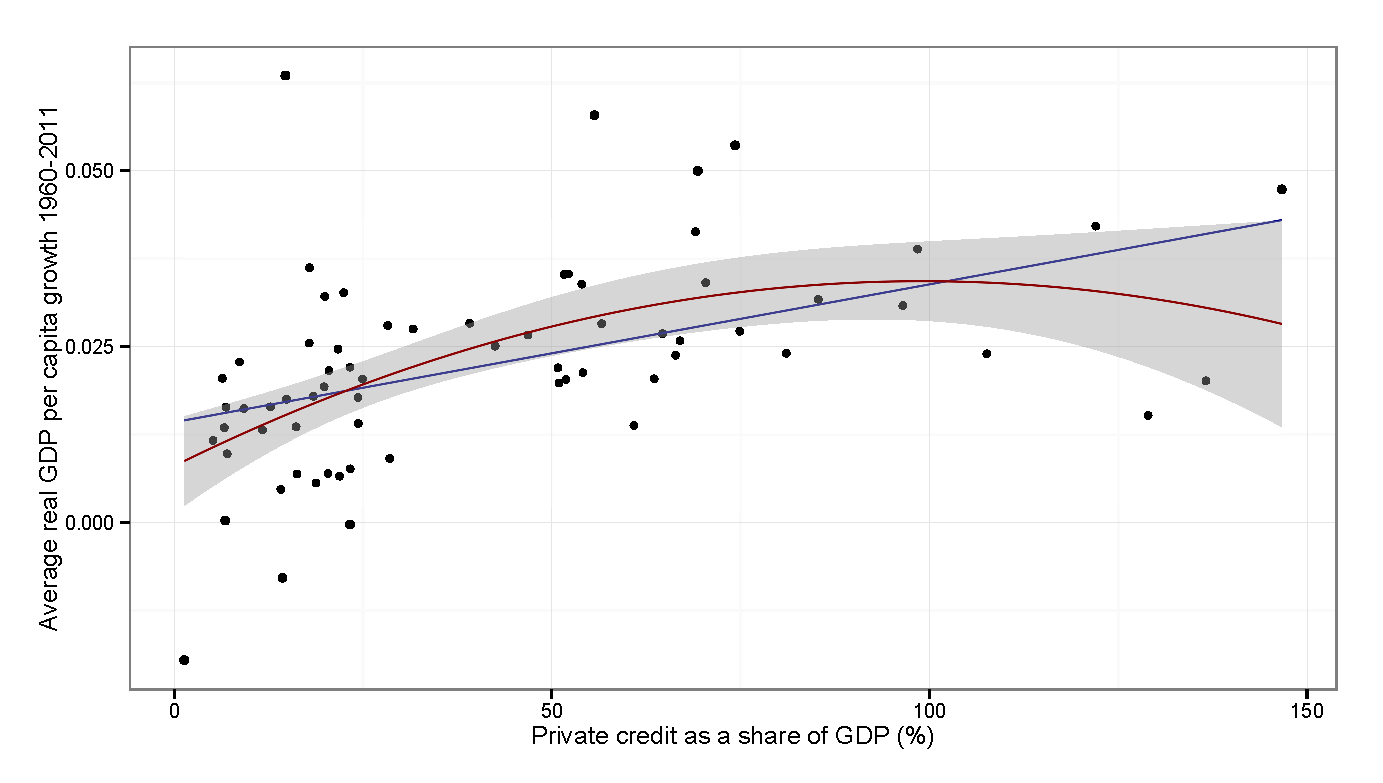
\includegraphics[width=\linewidth]{Figures/ch2/PConGDP1960-2011.eps}
		\caption{Private credit and growth, 1960-2011}
		\label{ch2fig:OLSPCGDP}
	\end{center}
\end{figure}

Table \ref{ch2tab:PC6011hyp} presents our baseline results for private credit. We sort the explanatory variables according to their \acp{PIP}. We find that the initial level of \ac{GDP} in 1960, the dummy variable for Sub-Sahara, the share of GDP in mining, the fraction of Confucian population, equipment investment, distortions in the exchange rate, and covariates capturing black market characteristics exhibit the highest \acp{PIP}. These findings are broadly in accord with the specification from \textcite{Fernandezetal2001} despite the choice of an alternative parameter prior and the consideration of an extended period. 
%
% Results, average financial indices 1960-2011; baseline results
\begin{table}[!ht]
	\centering
	\caption{Private credit and growth, baseline results\\
		Bayesian model averaging}
	\label{ch2tab:PC6011hyp}
	\small
	\begin{tabular}{lrrr}
		\toprule
		& PIP & Post Mean & Post SD \\ 
		\toprule
		Life expectancy & 1.00 & 0.00078 & 0.00023 \\ 
		GDP level in 1960 & 1.00 & -0.01330 & 0.00234 \\ 
		Fraction GDP in mining & 1.00 & 0.05972 & 0.01369 \\ 
		Fraction Confucian & 1.00 & 0.04527 & 0.01146 \\ 
		Black market premium & 1.00 & -0.01040 & 0.00327 \\ 
		Exchange rate distortions & 0.99 & -0.00009 & 0.00003 \\ 
		Sub-Sahara dummy & 0.99 & -0.01377 & 0.00539 \\ 
		SD of black market premium & 0.98 & 0.00003 & 0.00001 \\ 
		Equipment investment & 0.97 & 0.11111 & 0.04474 \\ 
		Fraction Buddhist & 0.84 & 0.00968 & 0.00653 \\ 
		Size of labor force & 0.75 & 7.1e-08 & 6.4e-08 \\ 
		French colony dummy & 0.64 & 0.00405 & 0.00402 \\ 
		Fraction Muslim & 0.53 & 0.00445 & 0.00529 \\ 
		Fraction of pop. speaking English & 0.48 & -0.00335 & 0.00445 \\ 
		Non-equipment investment & 0.38 & 0.01197 & 0.01942 \\ 
		Latin America dummy & 0.28 & -0.00152 & 0.00299 \\ 
		Rule of law & 0.24 & 0.00169 & 0.00388 \\ 
		Fraction Hindu & 0.16 & -0.00349 & 0.01138 \\ 
		Ethnolinguistic fractionalization & 0.16 & 0.00090 & 0.00268 \\ 
		Absolute latitude & 0.13 & 0.00002 & 0.00005 \\ 
		Fraction speaking foreign language & 0.11 & 0.00038 & 0.00144 \\ 
		Fraction Catholic & 0.10 & 0.00041 & 0.00180 \\ 
		British colony dummy & 0.09 & 0.00026 & 0.00133 \\ 
		Ratio of workers to population & 0.08 & 0.00059 & 0.00295 \\ 
		Public education share & 0.08 & 0.00754 & 0.03897 \\ 
		\textbf{Private credit} & \textbf{0.07} & \textbf{0.00025} & \textbf{0.00138} \\ 
		Number of years of open economy & 0.06 & -0.00030 & 0.00179 \\ 
		Spanish colony dummy & 0.06 & -0.00016 & 0.00115 \\ 
		Fraction Jewish & 0.05 & 0.00045 & 0.00319 \\ 
		Primary school enrollment & 0.05 & 0.00027 & 0.00214 \\ 
		Fraction Protestant & 0.04 & -0.00006 & 0.00108 \\ 
		Degree of capitalism & 0.04 & 0.00002 & 0.00018 \\ 
		Age & 0.03 & -5.5e-07 & 0.00001 \\ 
		Outward orientation & 0.03 & -0.00004 & 0.00043 \\ 
		High school enrollment & 0.03 & -0.00029 & 0.00572 \\ 
		Area & 0.03 & 4.9e-09 & 9.7e-08 \\ 
		Revolutions and coups & 0.03 & -0.00005 & 0.00083 \\ 
		Civil liberties & 0.03 & -0.00001 & 0.00019 \\ 
		War dummy & 0.03 & -0.00001 & 0.00036 \\ 
		Primary exports & 0.03 & -0.00001 & 0.00083 \\ 
		Population growth & 0.02 & 0.00032 & 0.02622 \\ 
		Political rights & 0.02 & -2.2e-06 & 0.00014 \\
		\bottomrule
	\end{tabular}
\end{table}
%

Although private credit ranks near the middle of the list of explanatory variables and its mean value of the coefficient is positive, the \ac{PIP} is only 7\%. This result indicates that credit is unlikely included as the explanatory variable in the "true" growth model. Overall, we find very limited support for the notion that financial depth is important for long-term economic growth.

In the baseline estimation, we follow \textcite{Fernandezetal2001} and use a uniform model prior. However, we depart from that study in the selection of the parameter prior. Instead of using the \ac{BRIC} prior, we employ the hyper-g prior, as the literature now considers it superior. The essential disadvantage of employing the \ac{BRIC} prior is documented by \textcite{FeldkircherZeugner2009}. They describe a phenomenon of a "supermodel effect", arguing that with a high fixed prior $g$, the shrinkage-factor $\frac{g}{1+g}$ in equation \ref{ch2eq:MLg} increases, thus increasing the size penalty, and may skew the posterior model distribution to smaller models. This choice of a large $g$ under fixed priors can result in a preference for overly simplistic models. According to \textcite{FeldkircherZeugner2009}, the phenomenon is characteristic of \ac{BMA} applications to growth regressions with numerous covariates. They further claim that using a model-specific hyper-g prior leads to more robust estimates. This is why we abstain from employing the \ac{BRIC} prior and focus on alternative options for parameter priors in our robustness checks.

The birth-death MC$^{3}$ sampler described in section \ref{ch2sec:mc3} is our preferred approach for approximating the \ac{PMP} distribution. To ensure sufficient convergence of the sampler, we specify 15 million iterations with 3 million  initial burn-ins. The full estimation diagnostics is available upon request. The average number of regressors included in the model is 19.09, and the correlation between analytical and sampler \ac{PMP} stands at 0.56. We realize that this \ac{PMP} correlation is far from ideal, but estimation with higher iteration counts and subsequently higher \ac{PMP} correlation yields nearly identical results.\footnote{Specifically, we ran the estimation using 50 million iterations and 5 000 000 burn-ins to arrive at a \ac{PMP} correlation of 0.82. Characteristics in terms of mean model size and \acp{PIP} remain virtually the same.} Note that below, we employ different parameters and model prior structures and achieve a \ac{PMP} close to 1, while the \acp{PIP} remain largely unchanged. 

Next, we examine whether the baseline results are robust to different parameter priors. \textcite{CicconeJarocinski2010} posit that \ac{BMA} results are sensitive to data revisions under certain prior structures. \textcite{Eicheretal2011} find that the \acp{PIP} of some growth determinants depend on the chosen parameter prior. Therefore, we perform the estimation using \ac{UIP}. We also check the robustness of the MC$^{3}$ sampler using the "reverse-jump" algorithm and the model prior by employing a random binomial model prior (see \textcite{Zeugner2011} for details).

The model comparison for different parameter priors and MC$^{3}$ algorithms is depicted in Figure \ref{ch2fig:compPC}. Model 1 includes the \acp{PIP} under our baseline specification. Model 2 employs the same priors but applies the "reverse-jump" MC$^{3}$ algorithm. Models 3 and 4 yield the results when we use \ac{UIP} under the birth-death and reverse-jump samplers, respectively. Though employing the reverse-jump sampler only marginally alters the \acp{PIP}, switching to the \ac{UIP} prior leads to slightly lower inclusion probabilities and model size. Overall, these findings indicate that our baseline results are robust.

% 
% Model comparison, 1960-2011 PC
\begin{figure}[!ht]
	\begin{center}
		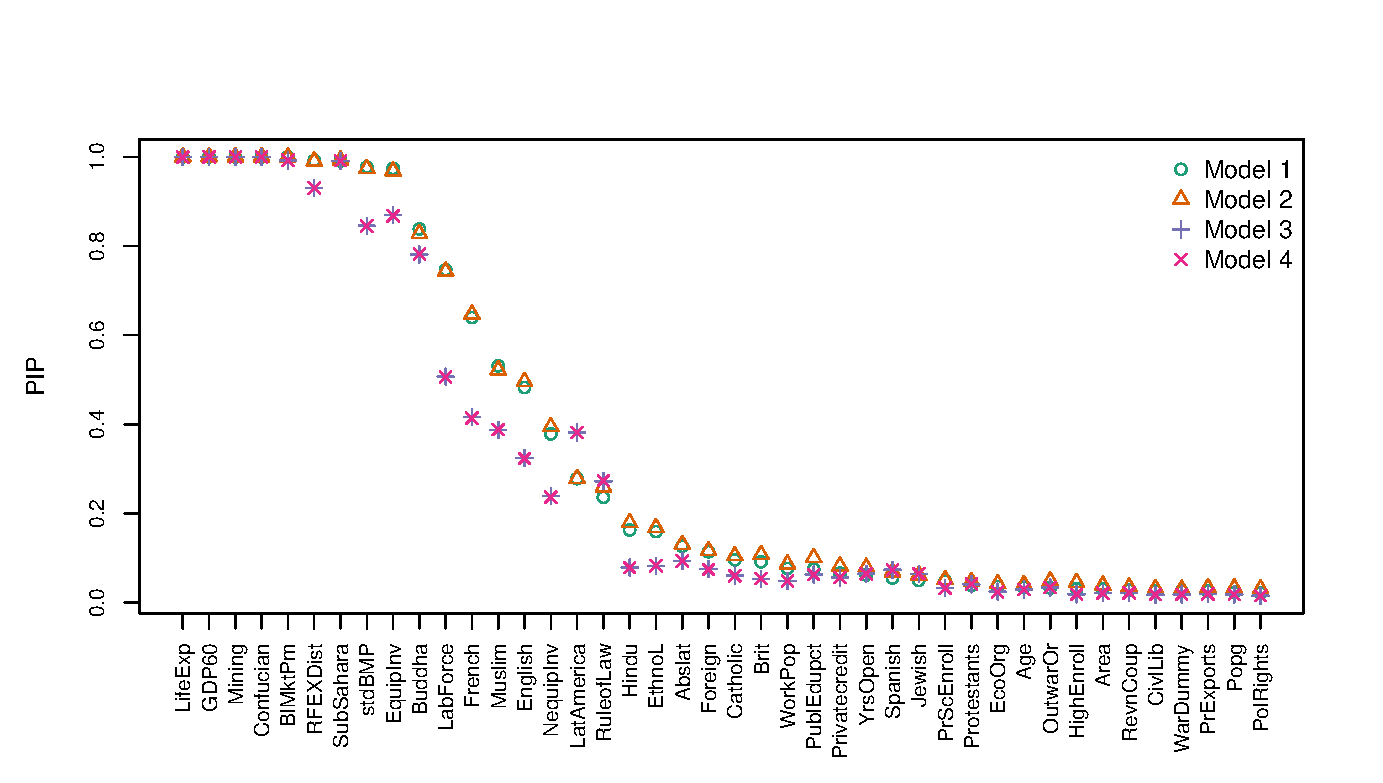
\includegraphics[width=\linewidth]{Figures/ch2/plotCompPC6011}
		\caption{Model comparison with private credit, Model 1=hyper-g,birth-death; Model 2=hyper-g,reverse-jump; Model 3=\ac{UIP},birth-death; Model 4=\ac{UIP},reverse-jump}
		\label{ch2fig:compPC}
	\end{center}
\end{figure}
%

The beta-binomial ("random") model prior offers meaningful insights. This setting allows for a less restrictive selection of model priors around the prior expected model size and limits the risk of imposing any particular one \parencite{LeySteel2009}. Thus, if the true model size is lower than that expected by the prior (21), we should expect the mean model size to decline in this setting. 
%
We present the results of the estimation using this model prior in Figure \ref{ch2fig:compPCrnd} in the Appendix. In the first setting with a hyper-g prior, the mean size declines to 15.05 and the PMP correlation between analytical and MC$^{3}$ sampler likelihood achieves a satisfactory value of 0.96. The most important variables according to their \acp{PIP} remain nearly unchanged, although their relative positions adjust. One significant change is the decline in the PIP of the volatility of the black market premium to 14\%. Finally, the inclusion probability of private credit increases marginally to 9\%. 

We also limit the period under consideration to 1960-1990 and examine whether the effect of financial development is stronger for this time period, as suggested by \textcite{RousseauWachtel2011}. We find that none of these modifications substantially affects our primary results concerning the relationship between private credit and economic growth.  The PIP of private credit estimated on the subsample before 1990 does not appear to differ from that obtained for the full period up to 2011. As a robustness check of our results, we also use the values of private credit from the beginning of the observed period instead of the averages, but we find that the coding change has a negligible effect. These results are available upon request.

\subsection{New Financial Development Indicators}
We examine the effect of new financial indicators on long-term growth in this subsection. Specifically, we additionally include the following variables in our estimation: bank Z-score, net interest margin, stock market turnover, and stock market capitalization. \textcite{Cihaketal2013} identify these as proxies for different aspects of the financial sector. Specifically, they propose using bank Z-score to assess the stability of the banking sector, the net interest margin to proxy for the efficiency of the banking sector, stock market turnover as a proxy for the efficiency of the stock market, and stock market capitalization to measure the depth of stock markets. These measures, particularly the first two, are rarely used in growth regressions (\textcite{Bergeretal2004} and \textcite{Hasanetal2009} being the exceptions), despite the fact that they might better depict the relationships outlined by theory than traditionally employed variables. As we discuss in section \ref{ch2sec:data}, the main issue lies in their availability. However, the \ac{GFDD} provides a significant improvement in this regard, and many series are available since the late 1980s. In addition, we retain domestic credit to the private sector among the covariates to account for the overall size of the banking sector. Given the data limitations, our sample is reduced to 60 countries. For eight countries from our original sample used for private credit, at least one value of the new financial indicators is missing.

Figure \ref{ch2fig:allvarplot}  provides an initial examination of the interaction between individual financial indicators and economic growth. First, we observe a distinct inverse relationship between the net interest margin and economic growth. Second, bank Z-score and growth display only a marginally positive relationship. Third, market capitalization and market turnover appear to be positively related to growth, which is in line with \textcite{LevineZervos1998}. In addition, Table \ref{ch2tab:corrFI} provides the correlations among the financial indicators. The correlations are typically far from one, thus providing additional impetus to examine further measures of financial development in the growth regressions. In addition, we present the jointness statistics in the Appendix \ref{ch2app:joint}.
%
% Rest of the financial indicators 1960-2011
\begin{figure}[!ht]
	\begin{center}
		\setlength{\fboxsep}{0pt}
		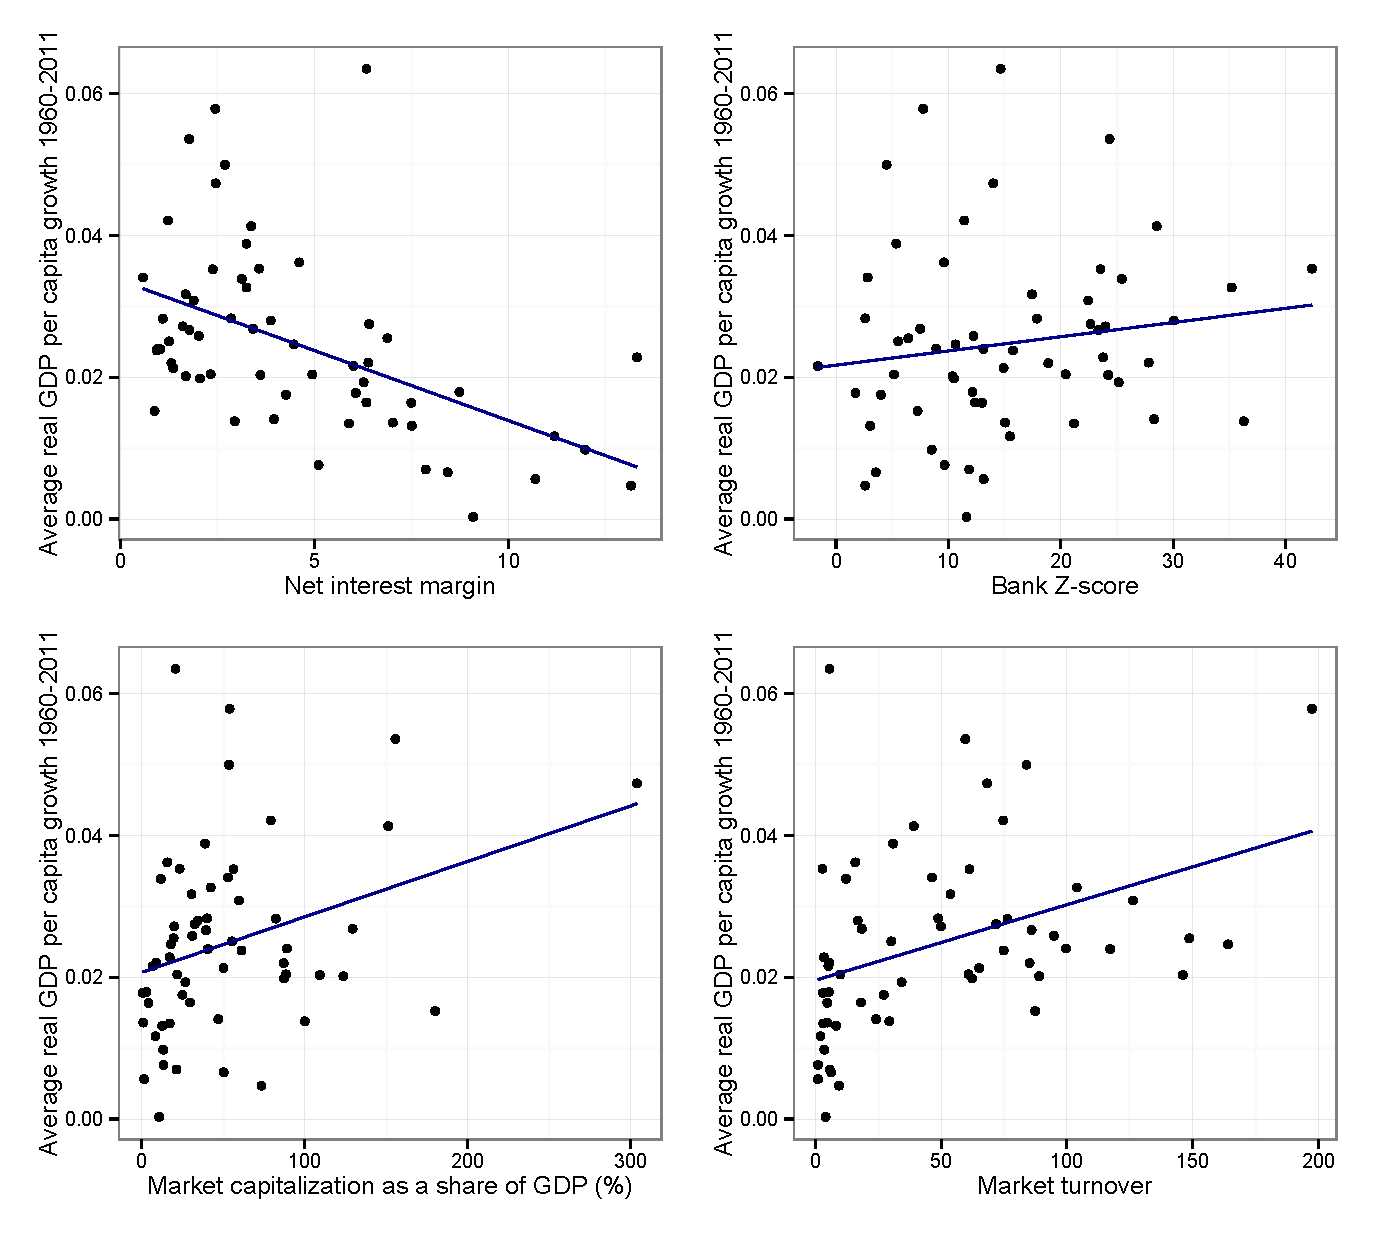
\includegraphics[width=\linewidth]{Figures/ch2/Plots60}
		\caption{Financial indicators and growth}
		\label{ch2fig:allvarplot}
	\end{center}
\end{figure}
%
% Correlation matrix of financial indicators
\begin{table}[!ht]
	\centering
	\caption{Correlation matrix of new financial indicators}
	\label{ch2tab:corrFI}
	\small
	\begin{tabular}{lrrrrr}
		\toprule
		Net interest margin & 1.00 & & & &                    \\ 
		Bank Z-score    & -0.14 & 1.00 &   &   &              \\ 
		Private credit & -0.71 & 0.03 & 1.00 &   &            \\ 
		Market capitalization & -0.44 & 0.08 & 0.71 & 1.00 &  \\ 
		Market turnover & -0.54 & 0.02 & 0.47 & 0.33 & 1.00   \\ 
		\bottomrule
	\end{tabular}
\end{table}
%

We report the results of the estimation in a similar fashion as we did for private credit. We retain the baseline specification with the hyper-g parameter prior, uniform model prior, and birth-death MC$^{3}$ sampler. The number of iterations remains at 15 million, and we specify 3 million burn-ins. The full estimation diagnostics is available upon request. As in the previous subsection, running more iterations does not affect the resulting \acp{PIP} and posterior means, although it leads to a higher convergence of the sampler. We primarily focus on the interpretation of the results concerning financial indicators, as the other explanatory variables' \acp{PIP} remain broadly similar to those of specification for private credit. 

%\clearpage
% All financial indicators, baseline results
\begin{table}[!htbp]
	\centering
	\caption{New financial indicators and growth 1960-2011, baseline results}
	\label{ch2tab:all6011hyp}
	\small
	\begin{tabular}{lrrr}
		\toprule
		& PIP & Post Mean & Post SD \\ 
		\midrule
		GDP level in 1960 & 1.00 & -0.01075 & 0.00234 \\ 
		Fraction GDP in mining & 1.00 & 0.04669 & 0.01338 \\ 
		Exchange rate distortions & 1.00 & -0.00009 & 0.00003 \\ 
		Fraction Confucian & 1.00 & 0.03896 & 0.01093 \\ 
		Life expectancy & 1.00 & 0.00057 & 0.00019 \\ 
		Fraction Buddhist & 0.98 & 0.01255 & 0.00497 \\ 
		\textbf{Net interest margin} & \textbf{0.97} & \textbf{-0.00115} & \textbf{0.00045} \\ 
		Equipment investment & 0.85 & 0.07432 & 0.04648 \\ 
		\midrule
		Fraction Protestant & 0.33 & -0.00225 & 0.00402 \\ 
		Ratio of workers to population & 0.33 & 0.00382 & 0.00671 \\ 
		\textbf{Bank Z-score} & \textbf{0.25} & \textbf{0.00004} & \textbf{0.00009} \\ 
		French colony dummy & 0.24 & 0.00183 & 0.00411 \\ 
		SD of black market premium & 0.22 & 3.1e-06 & 0.00001 \\ 
		Rule of law & 0.19 & 0.00139 & 0.00363 \\ 
		Outward orientation & 0.19 & -0.00050 & 0.00133 \\ 
		\textbf{Market turnover} & \textbf{0.17} & \textbf{0.00001} & \textbf{0.00002} \\ 
		Size of labor force & 0.12 & 6.6e-09 & 2.6e-08 \\ 
		Spanish colony dummy & 0.12 & 0.00054 & 0.00192 \\ 
		Fraction of pop. speaking English & 0.11 & -0.00044 & 0.00168 \\ 
		Fraction Jewish & 0.08 & 0.00093 & 0.00423 \\ 
		Fraction Muslim & 0.08 & 0.00033 & 0.00158 \\ 
		\textbf{Private credit} & \textbf{0.07} & \textbf{0.00028} & \textbf{0.00145} \\ 
		Fraction Catholic & 0.07 & -0.00025 & 0.00139 \\ 
		Primary exports & 0.06 & 0.00020 & 0.00135 \\ 
		Absolute latitude & 0.05 & 4.2e-06 & 0.00003 \\ 
		Fraction Hindu & 0.05 & -0.00048 & 0.00435 \\ 
		Fraction speaking foreign language & 0.05 & 0.00009 & 0.00068 \\ 
		Population growth & 0.04 & -0.00554 & 0.04705 \\ 
		Number of years of open economy & 0.04 & 0.00011 & 0.00093 \\ 
		Age & 0.04 & -6.6e-07 & 0.00001 \\ 
		War dummy & 0.04 & -0.00005 & 0.00047 \\ 
		High school enrollment & 0.04 & -0.00061 & 0.00575 \\ 
		Latin America dummy & 0.04 & -0.00006 & 0.00079 \\ 
		Black market premium & 0.04 & 0.00010 & 0.00101 \\ 
		Non-equipment investment & 0.04 & -0.00040 & 0.00408 \\ 
		Political rights & 0.04 & 0.00002 & 0.00018 \\ 
		British colony dummy & 0.04 & -0.00001 & 0.00045 \\ 
		Area & 0.03 & 7.9e-09 & 8.9e-08 \\ 
		Degree of capitalism & 0.03 & 0.00002 & 0.00019 \\ 
		Public education share & 0.03 & 0.00078 & 0.01915 \\ 
		Revolutions and coups & 0.03 & -0.00005 & 0.00076 \\ 
		Sub-Sahara dummy & 0.03 & -0.00001 & 0.00087 \\ 
		Primary school enrollment & 0.03 & -0.00007 & 0.00129 \\ 
		Ethnolinguistic fractionalization & 0.03 & -0.00001 & 0.00064 \\ 
		\textbf{Market capitalization} & \textbf{0.02} & \textbf{1.1e-07} & \textbf{3.3e-06} \\
		Civil liberties & 0.02 & 0.00001 & 0.00016 \\ 
		\bottomrule 
	\end{tabular}
\end{table}

We present the posterior statistics of the explanatory variables in Table \ref{ch2tab:all6011hyp}. Interestingly, the variable proxying for bank efficiency exhibits a comparatively higher \ac{PIP} than that reflecting its depth. Net interest margin ranks high among the explanatory variables with a 97\% inclusion probability. The posterior mean of the coefficient is negative, in accordance with our expectations. A lower interest margin stems from a smaller discrepancy between banks' borrowing and lending rates. Thus, if banks are able to channel resources at a lower margin, this appears to positively affect long-term economic growth \parencite{Rousseau1998}. Additionally, the posterior mean of bank Z-score is positive, implying that stable banking systems are beneficial for economic growth, although the \ac{PIP} at 25\% does not offer much confidence that the Z-score is a crucial determinant of long-term growth. Stock market turnover is also accorded little importance, with a \ac{PIP} of 17\%. The positive sign of the mean is in line with our expectations regarding an efficient resource allocation being beneficial for growth. Moreover, it supports the conclusion of \textcite{LevineZervos1998} that an active stock market contributes to economic growth. However, we wish to note that this indicator might not coherently capture the efficiency of the markets. A high turnover ratio could reflect low friction in trading and the spread of information \parencite{Levine2005}. On the other hand, other research finds that more trading does not necessarily prevent asset price misalignments and its corrections \parencite{Brunnermeier2004}. Strikingly, the measures capturing the depth of both the banking sector and stock markets exhibit very small \acp{PIP}. Overall, our results indicate that the approach used to measure financial development is crucial in determining the estimated effect of finance on growth. 

\begin{table}[!htbp]
	\centering
	\caption{New financial indicators and growth 2000-2011, baseline results\\
		Bayesian model averaging}
		\label{ch2tab:BMAgrowth2000-2011}
	\small
	\begin{tabular}{lrrr}
		\toprule
		& PIP & Post Mean & Post SD \\ 
		\midrule
		  Exchange rate distortions & 1.00 & 0.00022 & 0.00004 \\ 
		  War dummy & 1.00 & 0.01149 & 0.00290 \\ 
		  \textbf{Net interest margin} & \textbf{1.00} & \textbf{-0.00212} & \textbf{0.00055} \\ 
		  Primary exports & 1.00 & 0.01699 & 0.00496 \\ 
		  Fraction Confucian & 1.00 & 0.04151 & 0.01130 \\ 
		  Non-equipment investment & 1.00 & -0.09469 & 0.02661 \\ 
		  Political rights & 1.00 & 0.00641 & 0.00152 \\ 
		  Latin America dummy & 1.00 & 0.01679 & 0.00470 \\ 
		  Fraction GDP in mining & 1.00 & 0.08843 & 0.01789 \\ 
		  Ratio of workers to population & 1.00 & 0.04116 & 0.00919 \\ 
		  Revolutions and coups & 1.00 & -0.03279 & 0.00649 \\ 
		  Outward orientation & 1.00 & 0.00900 & 0.00261 \\ 
		  Sub-Sahara dummy & 1.00 & -0.03589 & 0.00910 \\ 
		  Fraction Hindu & 0.94 & 0.03725 & 0.01387 \\ 
		  SD of black market premium & 0.88 & 0.00003 & 0.00002 \\ 
		  \textbf{Private credit} & \textbf{0.53} & \textbf{-0.00003} & \textbf{0.00004} \\ 
		  Life expectancy & 0.31 & 0.00011 & 0.00021 \\ 
		  High school enrolment & 0.25 & -0.00932 & 0.02257 \\ 
		  \textbf{Bank Z-score} & \textbf{0.21} & \textbf{-0.00004} & \textbf{0.00010} \\ 
		  Rule of law & 0.16 & 0.00106 & 0.00369 \\ 
		  French colony dummy & 0.15 & -0.00091 & 0.00311 \\ 
		  Degree of capitalism & 0.14 & 0.00014 & 0.00055 \\ 
		  Size of labour force & 0.13 & 1.3e-08 & 5.0e-08 \\ 
		  Black market premium & 0.12 & 0.00084 & 0.00375 \\ 
		  Spanish colony dummy & 0.11 & -0.00046 & 0.00250 \\ 
		  Civil liberties & 0.10 & -0.00018 & 0.00096 \\ 
		  Number of years of open economy & 0.09 & 0.00034 & 0.00206 \\ 
		  Age & 0.09 & 1.1e-06 & 0.00001 \\ 
		  GDP level in 2000 & 0.09 & 0.00009 & 0.00076 \\ 
		  British colony dummy & 0.08 & 0.00004 & 0.00079 \\ 
		  Public education share & 0.08 & 0.00470 & 0.03815 \\ 
		  Absolute latitude & 0.08 & 4.3e-06 & 0.00003 \\ 
		  Fraction Muslim & 0.08 & 0.00035 & 0.00215 \\ 
		  Population growth & 0.08 & -0.00603 & 0.07020 \\ 
		  \textbf{Market capitalization} & \textbf{0.07} & \textbf{3.8e-07} & \textbf{4.7e-06} \\ 
		  Fraction Buddhist & 0.07 & -0.00021 & 0.00167 \\ 
		  Fraction Catholic & 0.07 & -0.00012 & 0.00102 \\ 
		  Ethnolinguistic fractionalization & 0.07 & 0.00028 & 0.00171 \\ 
		  Primary school enrolment & 0.07 & 0.00026 & 0.00278 \\ 
		  \textbf{Market turnover} & \textbf{0.07} & \textbf{4.5e-07} & \textbf{3.7e-06} \\ 
		  Fraction Jewish & 0.07 & 0.00017 & 0.00230 \\ 
		  Area & 0.07 & 1.3e-08 & 1.3e-07 \\ 
		  Fraction speaking foreign language & 0.07 & 0.00011 & 0.00089 \\ 
		  Fraction Protestants & 0.06 & 0.00007 & 0.00107 \\ 
		  Fraction of pop. speaking English & 0.05 & -0.00011 & 0.00103 \\ 
		  Equipment investment & 0.04 & 0.00026 & 0.00815 \\ 
		\bottomrule
	\end{tabular}
\end{table}

To provide robustness checks, we again perform the estimation with alternative priors.\footnote{We also perform estimations using an alternative MC$^{3}$ sampler, but the differences in posterior statistics are marginal.} Figure \ref{ch2fig:compall60} illustrates the comparison. The implications of different priors are similar to those experienced in the estimation regarding private credit. The \ac{UIP} parameter prior subtly alters the \ac{PIP} of the covariates without having a major effect on the interpretation. Providing greater flexibility in selecting model size by assuming a random model prior reduces the posterior mean model size and the \ac{PIP} of several variables, but the set of top-ranked regressors remains largely unchanged. The relative importance of financial indicators changes to some extent. Net interest margin remains among the most important variables with an 86\% \ac{PIP}. All the remaining indicators exhibit low \ac{PIP} below 10\%. This is due to the smaller size induced by the random model prior. The results using dilution prior which accounts for correlation among covariates decreases the \ac{PIP} of nearly all variables. However, the importance of net interest margin still remains high with the \ac{PIP} at 87\%.
% Model comparison, 1960-2011 findev
\begin{figure}[!ht]
	\begin{center}
		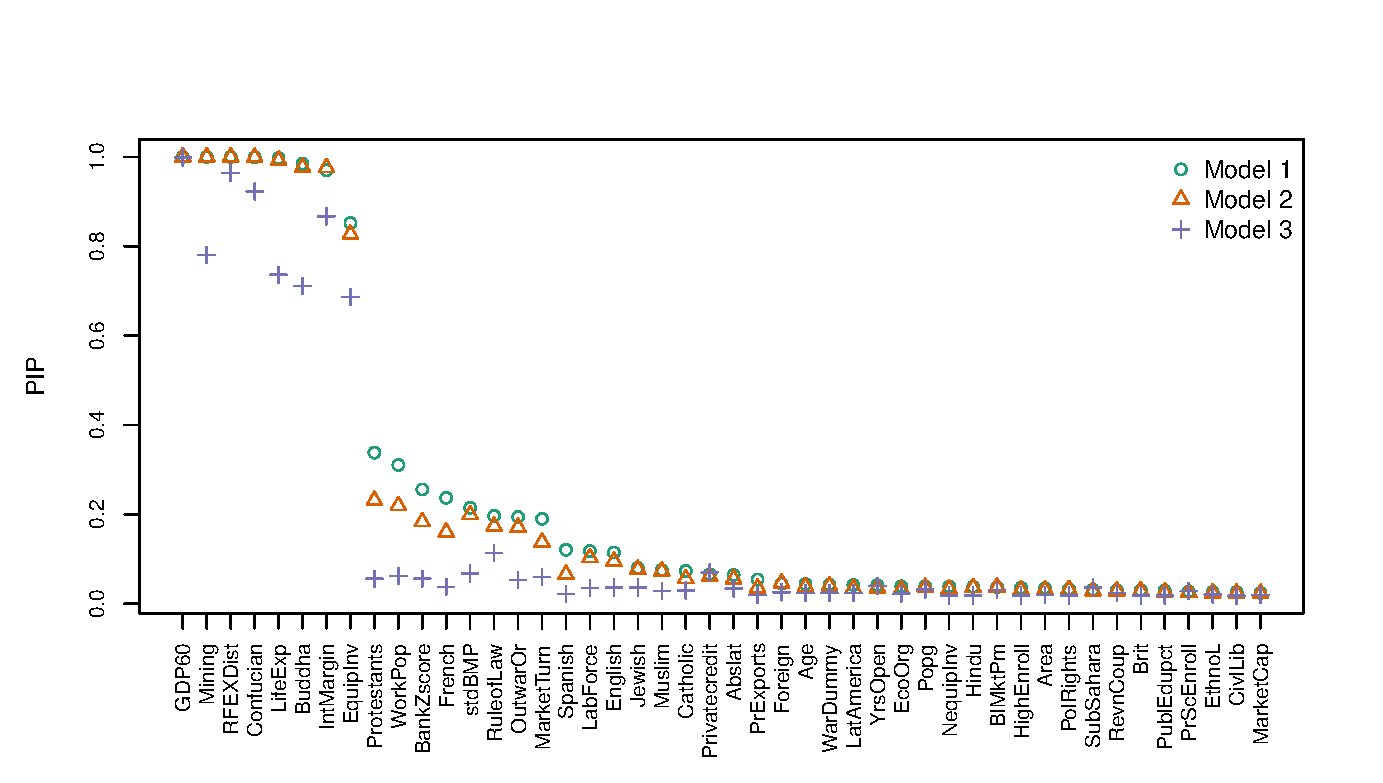
\includegraphics[width=\linewidth]{Figures/ch2/plotCompall6011}
		\caption{Model comparison with all financial indicators 1960-2011, priors Model 1=hyper-g, uniform model prior; Model 2=\ac{UIP}, uniform model prior, Model 3=hyper-g, dilution model prior}
		\label{ch2fig:compall60}
	\end{center}
\end{figure}

Our baseline estimations suggest that bank efficiency is crucial for growth. We perform an additional estimation to check the robustness of this finding. and estimate \ac{BMA} with lagged covariates. For reasons of data availability, we use real growth in GDP per capita over the period 2000--2011 and take the values of the financial indicators in the year 2000. The advantage of this approach is that we examine how past values of financial indicators influence current growth. Clearly, the disadvantage is that the time coverage for the dependent variable is restricted to just over a decade.\footnote{Alternatively, we also estimate 2SLS--\ac{BMA} regressions following the methodology of \textcite{Durlaufetal2008}, which consists of two steps. We regress the endogenous financial indicators on our set of instruments in the first stage. The fitted values of financial indicators enter into the second stage \ac{BMA} estimation. The results are largely in line with our baseline results and are available from the authors upon request.} Implicitly, this may also be regarded as robustness check of the sensitivity of our results to the variable coding. We present the results in Table \ref{ch2tab:BMAgrowth2000-2011}. Interestingly, the results remain largely unchanged. Net interest margin remains among the covariates with the highest \ac{PIP}. The posterior mean of the coefficient is negative. The \ac{PIP} of private credit is 49\%, but the mean is negative. We hypothesize that the negative mean is a consequence of our sample period including the current global financial crisis, which has been characterized by deleveraging in many developed countries. The \ac{PIP} of the other financial indicators is not high.

\subsection{Non--linearities in Finance and Growth Nexus}
Finally, we examine the possibility of a nonlinear relationship between financial indicators and growth. Several recent studies on financial development and economic growth devote substantial attention to nonlinearities in the relationship between financial development and economic growth (see, for example, \textcite{CecchettiKharroubi2012, LawSingh2014}). In addition, we also examine several possible interaction effects in finance--growth nexus such as whether private credit is conducive to growth only when financial system is stable.

When considering the quadratic and interaction terms, we rely on the strong heredity principle to adjust prior model probabilities. This approach has been suggested in the literature to ensure appropriate interpretation of the results. In essence, the quadratic and interaction terms may only be evaluated when their linear counterparts are included in the model. Therefore, they cannot mask potential effects of linear terms. 

The results of the specification focused only on private credit do not alter our conclusions from the basic linear setup. The posterior inclusion probabilities of private credit and its quadratic term are 8\% and 1\%, respectively.\footnote{In this subsection we report only the posterior statistics of the financial variables. The full results including the other variables are available upon request.} Next, we present the results with all financial indicators in Table \ref{ch2fig:BMAquad}. The \acp{PIP} on the linear terms are similar to the ones in the baseline linear specification from the previous subsection. The \ac{PIP} on the net interest margin remains high at 88\%. At the same time, we find very low posterior inclusion probabilities for all the quadratic terms with the exception of the net interest margin, which stands at 38\%. While this value is not higher than sometimes suggested cut-off threshold of 50\%, it provides some weak evidence for decreasing marginal returns of our efficiency indicator. 

\begin{table}[!htbp]
	\centering
	\caption{New financial indicators and quadratic terms\\
		Bayesian model averaging}
		\label{ch2fig:BMAquad}
	\small
	\begin{tabular}{lrrr}
		\toprule
		& PIP & Post Mean & Post SD \\ 
		\midrule
		  Net interest margin & 0.88 & -0.00192 & 0.00155\\ 
		  Net interest margin sq. & 0.38 & 0.00006 & 0.00010\\ 
		  Market turnover & 0.20 & 0.00003 & 0.00009\\ 
		  Bank Z-score & 0.19 & 0.00003 & 0.00009\\ 
		  Market turnover sq. & 0.12 & -1.3e-07 & 4.0e-07 \\ 
		  Private credit & 0.09 & 0.00001 & 0.00005\\ 
		  Private credit sq. & 0.03 & -4.4e-08 & 2.7e-07 \\ 
		  Market capitalization & 0.01 & -2.1e-07 & 4.7e-06 \\ 
		  Bank Z-score sq. & 0.01 & 1.3e-07 & 1.4e-06 \\ 
		  Market capitalization sq. & 0.00 & 6.6e-10 & 1.7e-08 \\
		\bottomrule
	\end{tabular}
\end{table}

\begin{table}[!htbp]
	\centering
	\caption{New financial indicators and interaction terms\\
		Bayesian model averaging}
		\label{ch2fig:BMAint}
	\small
	\begin{tabular}{lrrr}
		\toprule
		& PIP & Post Mean & Post SD \\ 
		\midrule
		  Net interest margin & 0.95 & -0.00110 & 0.00050 \\
		  Bank Z-score & 0.29 & 0.00005 & 0.00010 \\
		  Market turnover & 0.18 & 0.00001 & 0.00002 \\
		  Private credit & 0.08 & 2.8e-06 & 0.00002 \\
		  Market capitalization & 0.03 & 2.1e-07 & 4.8e-06\\
		  Bank Z-score*Net interest margin & 0.02 & 5.8e-07 & 5.9e-06 \\
		  Net interest margin*Private credit & 0.00 & 3.8e-08 & 1.4e-06\\
		  Bank Z-score*Private credit & 0.00 &-5.4e-10 & 6.9e-08 \\
		\bottomrule
	\end{tabular}
\end{table}

Finally, we report the results on the interaction terms. In the estimation we take the baseline scenario with all financial indicators and augment it with the interactions between private credit (depth), bank Z-score (stability), and net interest margin (efficiency). Table \ref{ch2fig:BMAint} summarizes the results. While the \acp{PIP} for the linear terms of financial indicators remain largely unchanged, the \acp{PIP} for the examined interaction terms are close to zero.

\section{Conclusions}
\label{ch2sec:conclusions}
We contribute to the voluminous finance and economic growth literature in two ways. First, we use Bayesian model averaging \parencite{Rafteryetal1997}. This methodology is firmly grounded in statistical theory and allows the researcher to jointly evaluate a large number of potential covariates considered in the literature. This is important because we know that regression model uncertainty in growth regressions is high \parencite{SalaiMartinetal2004,Durlaufetal2008} and there are numerous potential determinants of growth that could be included. Without considering model uncertainty, researchers examining the finance-growth nexus risk omitted variable bias and inconsistently estimated parameters. 

Second, the previous literature examining the finance-growth nexus largely employs measures of financial depth (for both the banking sector and stock markets) but rarely examines measures of the efficiency of financial intermediaries or financial stability. For this reason, we use newly developed financial indicators from the World Bank's \ac{GFDD}. These indicators capture not only depth but also efficiency and stability. It is vital to revisit the finance and growth literature because recent studies report that excessive financial development harms growth \parencite{CecchettiKharroubi2012}.

Using the updated well-known cross-country growth dataset by \textcite{Fernandezetal2001}, we find that traditional indicators of financial depth are not robustly related to long-term economic growth. The measures of financial depth and financial stability exhibit posterior inclusion probabilities well below 50\%. However, our results suggest that bank efficiency, as proxied by the net interest margin, is crucial for long-term growth. The corresponding posterior inclusion probability is on average around 90\%. This result is in line with theory, which indicates that the financial sector is essential in channeling resources from savers to borrowers \textcite{Pagano1993}. These results are robust to different parameter and model priors in Bayesian model averaging. The results are also robust once we address the endogeneity of financial indicators. In addition, we do not find non--linearities and various interaction effects (such as the effect of the interaction of credit and financial stability) important for finance--growth nexus. 

Overall, we find that the measurement of financial development is crucial in determining the estimated effect of finance on growth. Based on our global sample, the results attribute a greater role to the banking sector and its efficiency in fostering economic growth. Therefore, our results suggest that the quality of financial intermediation rather than the quantity of finance matters for growth. Our results thus stand in contrast to the recent papers suggesting that too much finance harms growth. We show that once we distinguish between quality and quantity of finance, we find that quality matters and quantity is largely irrelevant for long--term real growth. In terms of policy implications, our results indicate that the current wave of regulatory changes intended to safeguard financial stability should carefully analyze the consequences for the efficiency of financial intermediaries.

\newpage
% \fancyhead[LO]{\sffamily Bibliography}		%headers in sans serif and not in uppercase
% \bibliographystyle{Styles/Stylebib}			%style of literature, you can use e.g. newapa	instead of Styles/Stylebib
\printbibliography
\addcontentsline{toc}{section}{Bibliography}

\newpage

\section*{Appendix}
\begin{subappendices}
\section{Description of the Dataset}
We use a commonly employed dataset on the determinants of growth developed by \textcite{Fernandezetal2001}. The dataset contains 41 explanatory variables that are potentially important for growth in 72 countries. Here, we describe the variables that do not assess financial development. Financial indicators, which we add to this dataset, are described in the main text.

We update the dataset by incorporating economic growth from new \ac{PWT}, extending the time period considered from the former 1960-1992 to 1960-2011. Our dependent variable is the average growth of real output-based GDP per capita. The mean value of the growth rate across the dataset is 2.27\% with a standard deviation of 1.45\%. The regressors in the dataset comprise various measures of economic, political, geographic, demographic, social, and cultural factors. As many of the variables are endogenous with respect to growth, the data typically come from 1960 or before. 

The economic variables primarily capture established factors from neoclassical growth theories. The initial level of GDP is included to capture conditional convergence, such that lower starting levels imply higher growth rates \parencite{BarroandMartin1992}. Additionally, physical capital investment is considered, distinguishing between equipment investment (machinery) and non-equipment investment (other). This follows \textcite{DeLongandSummers1991}, who find that the impact of the former is a stronger driver of long-term economic growth. Human capital enters through primary school enrollment, higher education enrollment and public education share from \textcite{Barro1996}. Life expectancy is often assumed to capture human capital other than education; therefore, it is also included among the regressors. Exchange rate fluctuations, the black market premium, and the volatility of the black market premium account for the degree of economic uncertainty. Exchange rates can affect a country's foreign direct investments and net exports, subsequently influencing economic growth. The black market premium then reflects the surplus on the exchange rate over the official foreign exchange market. High discrepancy mirrors greater uncertainty, and in addition to high volatility, we expect it to decelerate growth. Moreover, a set of variables accounts for economic policies. Outward orientation based on an import-export structure reflects the potential impact of international competition on domestic production efficiency. Economic organization captures the degree of capitalism, using the classification developed by \textcite{HallJones1996}. The characteristic is measured on a six-degree scale ranging from "statist" to "capitalist" that depends on how much control the national government exerts over the economy. Finally, the degree of openness enters through the length of period that the country has experienced an open economy. All policy variables are assumed to be positively correlated with economic growth.

Geographic controls include dummy variables for Sub Saharan Africa, Latin America, total area, and absolute latitude. Spatial differences in economic growth have been established in the literature. The location of a country may influence growth through differences in transportation costs, disease burdens, or agricultural productivity \parencite{Gallupandsachs1999}. A location farther from the equator should have a positive impact on growth.

The explanatory variables measuring political conditions within countries are colonial heritage, rule of law, indices for political rights, civil rights, and revolutions and coups. Political instability is further captured by war dummy, which equals 1 if the country suffered from war during 1960-1992. \textcite{Acemogluetal2001} note that colonial heritage is related to lower trust and malfunctioning institutions; therefore, former colonial status depresses growth. The rule of law is an established control in growth regressions, proxying for security, property rights, democratic government, and corruption \parencite{HaggardTiede2011}. Civil liberties further accounts for the level of democracy and its relationship with income redistribution. If a large share of income is in the hands of a few, this may have consequences for economic agents' production incentives. Intuitively, revolutions and coups negatively affect growth by decreasing stability and infrastructure destruction.

The demographic characteristics of countries we use in our estimation are average age, religion, ethnolinguistic fractionalization, population growth, total labor force, ratio of workers in population, and language skills. Religion is found to be relevant to economic growth in \textcite{Barro1996}. Population growth accounts for the neoclassical implication of a, ceteris paribus, decline in per capita growth with an increasing population. Language skills are approximated by the fraction of persons speaking English within a country and the fraction of persons speaking a foreign language. \textcite{HallJones1996} demonstrate how better language skills are positively reflected in economic growth. They argue that this arises from facilitated internalization and the benefits of globalization. The full list of variable names and their abbreviations is presented below.

Additionally, \ac{PWT} is missing observations on Algeria, Haiti, and Nicaragua. Therefore, we have to drop them from the sample. Furthermore, the GFDD does not include data on Taiwan. Ultimately, we have 68 observations, encompassing both developed and developing countries. The list of countries is as follows: Argentina, Australia, Austria, Belgium, Bolivia, Brazil, Botswana, Canada, Chile, Cameroon, Congo (Brazzaville), Congo Dem. Rep (Kinshasa), Colombia, Costa Rica, Cyprus, Denmark, Dominican Republic, Ecuador, El Salvador, Ethiopia, Finland, France, United Kingdom, Germany, Ghana, Greece, Guatemala, Hong Kong, Honduras, India, Ireland, Israel, Italy, Jamaica, Jordan, Japan, Kenya, South Korea, Sri Lanka, Morocco, Madagascar, Mexico, Malawi, Malaysia, Nigeria, Netherlands, Norway, Pakistan, Panama, Peru, Philippines, Portugal, Paraguay, Senegal, Singapore, Spain, Sweden, Switzerland, Thailand, Tunisia, Turkey, Tanzania, Uganda, Uruguay, United States, Venezuela, Zambia, and Zimbabwe.

We use the following list of variables (the details on the construction of variables are available in \textcite{Fernandezetal2001}): Absolute latitude, Age, Area, Black market premium, British colony dummy, Fraction Buddhist, Fraction Catholic, Civil liberties, Fraction Confucian, Degree of capitalism, Fraction of population speaking English, Equipment investment, Ethnolinguistic fractionalization, Fraction speaking foreign language, French colony dummy, GDP level in 1960, High school enrollment, Fraction Hindu, Fraction Jewish, Size of labor force, Latin America dummy, Life expectancy, Fraction GDP in mining, Fraction Muslim, Non-equipment investment, Outward orientation, Political rights, Population growth, Primary exports, Fraction Protestant, Primary school enrollment, Public education share, Revolutions and coups, Exchange rate distortions, Rule of law, Spanish colony dummy, SD of black market premium, Sub-Sahara dummy, War dummy, Ratio of workers to population, Number of years of open economy, Bank Z-score, Net interest margin, Stock market capitalization to GDP, Stock market turnover ratio, and Domestic credit to private sector.

% Model comparison, 1960-2011 PC random model priors
\begin{figure}[!ht]
	\begin{center}
		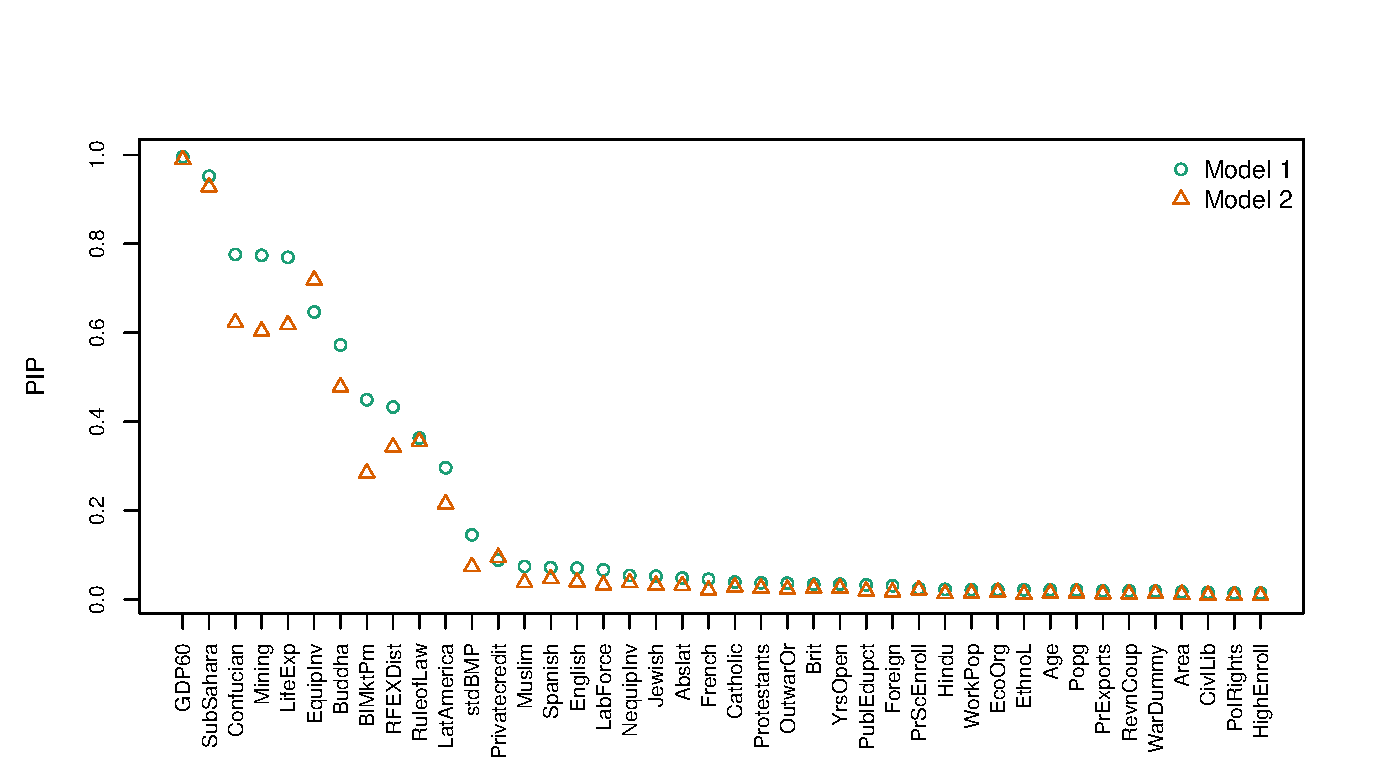
\includegraphics[width=\linewidth]{Figures/ch2/plotCompPC6011rnd}
		\caption{Model comparison with private credit, Model 1=hyper-g, random model prior; Model 2=\ac{UIP}, random model prior}
		\label{ch2fig:compPCrnd}
	\end{center}
\end{figure}
%

\section{Jointness of financial indicators}\label{ch2app:joint}
To check the dependence between our financial variables, we compute the so--called jointness measure, which is based on the posterior distributions of explanatory variables over the model space. The goal of this exercise is to determine whether the different financial variables capture different sources of information in explaining the dependent variable (jointness) or if they represent similar factors and should not be considered jointly in the model (disjointness) \parencite{leysteel2007}.

Jointness statistics for our financial indicators are available in Tables \ref{ch2tab:joint1}--\ref{ch2tab:joint3} with each table representing a different approach to jointness computation. Tables \ref{ch2tab:joint1} and \ref{ch2tab:joint2} show that none of the numbers exceeds the threshold suggested by \textcite{leysteel2007} (LS) for decisive (dis)jointness. Nevertheless, jointness statistics for some of the pairs suggest very strong jointness (e.g. market capitalization and private credit). Another way of constructing jointness statistic has been developed by \textcite{doppelhoferweeks2009} (DW). Regarding DW statistic, we find strong substitutability for private credit and net interest margin. However, as has been stressed by \textcite{leysteel2009b}, DW jointness statistic may become very sensitive and volatile if one of the variables has high \ac{PIP} and the other has a very low one. This is indeed the situation we encounter in our analysis. In addition, if the net interest margin and private credit were to be strong substitutes in a sense they would represent very similar factors and thus be mutually replaceable in the estimation process, they should also exhibit the same importance regarding economic growth if considered separately. These findings make us believe that the LS statistics are more appropriate to judge the interdependence between financial indicators.

\begin{table}[!htbp]
\caption{Financial indicators, jointness statistics according to \textcite{leysteel2007}}
\label{ch2tab:joint1}
\small
\centering
\begin{tabular}{llllll}
   \toprule
  Net interest margin & . & &  &  &  \\ 
  Bank Z-score & 0.335 & . & & & \\ 
  Private credit & 0.058 & 0.025 & . & &  \\ 
  Market capitalization & 0.025 & 0.014 & 0.011 & . & \\ 
  Market turnover & 0.224 & 0.158 & 0.041 & 0.027 & . \\ 
   \bottomrule
\end{tabular}
\end{table}

\begin{table}[!htbp]
\caption{Financial indicators, jointness statistic according to \textcite{leysteel2007}, alternative}
\label{ch2tab:joint2}
\small
\centering
\begin{tabular}{llllll}
   \toprule
  Net interest margin & . &  &  &  &  \\ 
  Bank Z-score & 0.251 & . &  &  &  \\ 
  Private credit & 0.055 & 0.024 & . &  &  \\ 
  Market capitalization & 0.024 & 0.013 & 0.011 & . &  \\ 
  Market turnover & 0.183 & 0.136 & 0.039 & 0.027 & . \\ 
   \bottomrule
\end{tabular}
\end{table}

\begin{table}[!htbp]
\caption{Financial indicators, jointness statistic according to \textcite{doppelhoferweeks2009}}
\label{ch2tab:joint3}
\small
\centering
\begin{tabular}{llllll}
   \toprule
  Net interest margin & . &  &  & & \\ 
  Bank Z-score & -0.372 & . &  &  & \\ 
  Private credit & \textbf{-2.373} & -1.025 & . &  & \\ 
  Market capitalization & 0.028 & -0.645 & -0.521 & . & \\ 
  Market turnover & -0.829 & 0.165 & -0.331 & 0.256 & . \\ 
   \bottomrule
\end{tabular}
\end{table}  
%
\end{subappendices}
\end{refsection}
% \begin{refsection}
\chapter{Finance and Wealth Inequality}
% \acresetall % resetting acronyms, spelled out in full on the first occurrence
\label{ch3}
\blfootnote{This chapter was co-authored with Iftekhar Hasan and Roman Horv\'{a}th and published in the \emph{Journal of International Money and Finance}. We thank Joshua Aizenman, Trinil Arimurti, Nauro Campos, Alex Cukierman, Michael Koetter, Lubos Pastor, Fabien Rondeau and Dimitrios Tsomocos for helpful discussions and seminar participants at the Annual International Conference on Macroeconomic Analysis and International Finance, European Public Choice Annual Conference, Financial Engineering and Banking Society Annual Conference, Multinational Finance Society Annual Conference, Charles University, Leibniz Institute for East and Southeast European Studies and University of Economics, Prague for helpful comments. Mares acknowledges the hospitality of Columbia University, where he stayed as visiting researcher in January-April 2018 thanks to the support by the H2020-MSCA-RISE project GEMCLIME-2020 GA No. 681228, and support from Grant Agency of Charles University No. 768217}

\begin{quote}
\begin{center}\textbf{Abstract}\end{center}
    Using a global sample, this paper investigates the determinants of wealth inequality capturing various economic, financial, political, institutional, and geographical indicators. Using instrumental variable Bayesian model averaging, it reveals that only a handful of indicators robustly matters and finance plays a key role. It reports that while financial depth increases wealth inequality, efficiency and access to finance reduce inequality. In addition, redistribution and education are associated with lower inequality whereas wars and openness to international trade contribute to greater wealth inequality.   
	\end{quote}

\clearpage
%
\section{Introduction}\label{ch3sec:intro}

Wealth inequality differs markedly across countries \parencite{daviesetal2011,daviesetal2017,milanovic2016global}. The wealth share of the top 1\% in the US is currently approximately 40\%, and it is even higher in Russia. On the other hand, the wealth share of the top 1\% is approximately 20\% in France and even lower in the UK \parencite{zucman2019}. What accounts for these (dramatic) differences in wealth inequality across countries? Is it different degrees of redistribution, financial development, globalization, technological progress or economic development? Alternatively, are there possibly some other factors? Although extensive progress has been made regarding the measurement of wealth inequality  \parencite{alvaredoetal2013,daviesetal2011,daviesetal2017,pikettyandzucman2014,SaezZucman2016}, we still lack systematic evidence about the determinants of wealth inequality across countries.

The theoretical models of wealth inequality suggest that several factors affect wealth inequality. The theoretical principles of the $r > g$ concept\footnote{This means that the rate of return on capital, $r$, exceeds economic growth, $g$.} laid out in \textcite{piketty2014} predict that there is a natural tendency of wealth inequality to increase in capitalist economies, which can be overcome only by redistribution or wars. This concept has received criticism from the theoretical point of view \parencite{blume2015capital,mankiw2015yes}.\footnote{See \textcite{king2017literature} for a review of the literature about the topic.} 

Dynamic quantitative models represent another approach to understand wealth inequality and focus on the heterogeneity of returns, preferences, transmission of human capital, and bequests. \textcite{DENARDI2017280} provide an overview of these models and their ability to mirror empirical wealth distributions. One of the conclusions is that all of the models critically rely on the saving motives of individuals. The theoretical predictions regarding wealth inequality arise from the model by \textcite{pastor2016income}, in which inequality depends on the skill and risk aversion of entrepreneurs, taxation, and the development of financial markets.\footnote{More specifically, it depends on the ability of entrepreneurs to diversify away their idiosyncratic risk, which can be interpreted as a measure of financial development.} Overall, the theoretical models postulate that several factors may matter for wealth inequality but do not provide a single theoretical framework to guide the exact regression model specifications. 

In this paper, we study the potential determinants of wealth distribution by relying on a global sample of countries and examining a wide array of possible determinants. Given that there is no encompassing theoretical framework, we propose to employ \ac{BMA} as our methodological framework. \ac{BMA} is a well-established approach within statistical theory and addresses the inherent regression model uncertainty in a unifying framework \parencite{Koopetal2007,Rafteryetal1997}.\footnote{\ac{BMA} has been applied to examine various issues in economics and finance, such as to study economic growth \parencite{Durlaufetal2008,Fernandezetal2001}, stock market predictability  \parencite{avramov,cremers}, intertemporal elasticity of substitution \parencite{Havraneketal2015}, exchange rate forecasting \parencite{wright} and interactions between credit spreads and economic activity \parencite{faust2013}.} 


In essence, the \ac{BMA} procedure evaluates different combinations of explanatory variables and weights the corresponding coefficients using the measure of model fit. In addition, \ac{BMA} is the perfect tool for the evaluation of numerous regressors and estimating their \ac{PIP}, the probability that a given regressor should be in the `optimal' model of wealth inequality. We address potential endogeneity within the estimation by using lagged values of explanatory variables and, more rigorously, by relying on the \ac{IVBMA} approach by \textcite{KarlLenkoski2012}.

Using our \ac{BMA} approach, we examine how 37 different factors explain the differences in cross-country wealth inequality among 73 countries. We focus on a number of economic, financial, institutional, regulatory, political and policy factors, such as education, financial development, government policies, technological progress, entrepreneurship and macroeconomic stability. To capture wealth inequality, we use the wealth Gini coefficient from \ac{CSWD}, constructed using the methodology of \textcite{daviesetal2017}. The \ac{CSWD} is the only available dataset with sufficient country coverage. We also add a set of indicators for financial development by \textcite{svirydzenka2016introducing}, which employ the most densely available series from \ac{GFDD} to capture various characteristics of financial systems. We include these measures to reflect the assumptions made by the theory, in which savings, which depend on financial markets, and financial development are the main drivers of wealth inequality.

Examining our global sample, we find that several factors are robustly related to wealth inequality. We find that financial development is an especially important determinant of wealth inequality across countries. Our results suggest that finance exerts a complex effect on wealth inequality. Whereas countries with more finance (i.e., large financial markets and financial institutions) exhibit greater wealth inequality, more efficiency and greater access to finance is associated with less wealth inequality. In general, this evidence supports the notion that sound financial systems contribute to lower wealth inequality. According to our results, the empirical importance of finance for wealth inequality suggests that theoretical models should more thoroughly examine the complex links between finance and wealth.

Our results also suggest that education reduces wealth inequality. Education decreases the gap between the wealthy and poor, corresponding to the findings by \textcite{dabla2015causes} regarding the determinants of income inequality.\footnote{However, note that the theoretical effect of education on inequality is ambiguous. \textcite{scheidel} discusses the channels via which education -- primarily through assortative mating and the elite school system being disproportionally less accessible to children from poor families -- amplifies inequality.} Wealth inequality is also lower in countries with more redistribution, as measured by the difference between the market and after-tax income Gini coefficients. Finally, globalization, as proxied by trade openness, and the extreme form of political instability, as proxied by the number of wars, tend to increase wealth inequality. 

The remainder of the paper is organized as follows. Section \ref{ch3sec:literature} reviews the literature on wealth inequality. Section \ref{ch3sec:data} presents the data, and \ref{ch3sec:BMA} introduces the \ac{BMA}. We provide the results in section \ref{ch3sec:results} and conclude in section \ref{ch3sec:conclusion}. Additional robustness checks are available in Section \ref{ch3sec:app_rch} in the Appendix.
%
%
%
%
%
\section{Related literature}\label{ch3sec:literature}
%\subsection{Quantitative models of the distribution of wealth}
Wealth inequality is typically analyzed within the theoretical framework of \textcite{bewley1977permanent} and \textcite{Ayiagari1994}. This framework relaxes the assumption of efficient economies and allows for, among other aspects, incomplete markets. The agents within the economy face a stochastic process of labor earnings and optimize consumption-saving behavior in incomplete markets. Additional specifications include restrictions on saving assets or borrowing constraints. Among other macroeconomic phenomena, the models can help us to understand the dynamics of the equilibrium distributions of consumption, savings, and wealth \parencite{BENHABIB2015489}.

The basic mechanism in the Bewley model relies on the environment in which agents save to self-insure against idiosyncratic labor-earning shocks. This precautionary motive to save is the primary driver of wealth accumulation. The basic version of the model has severe limitations. The ability to self-insure increases with the wealth/earnings ratio. The saving rate thus decreases and eventually turns negative if individual wealth is sufficiently greater than labor earnings. In other words, the basic setup implies negative saving rates for the rich. It also overstates the fraction of the population that does not save at all. These features of the model are in contrast with the data in \ac{US}, in which we observe high saving rates for the rich, and the share of agents without savings is very small \parencite{DENARDI2017280}. 

For this reason, the saving motives are extended to account more accurately for the actual dynamics of wealth accumulation and distribution. Some of the extensions introduce bequests and the transmission of human capital across generations \parencite{nardi2004wealth,de2014bequests}, heterogeneity in both time preferences and risk aversion \parencite{HENDRICKS2007}, earnings risk \parencite{castaneda2003}, saving for out-of-pocket medical expenses \parencite{kopecky2014impact}, heterogeneity in rates of return \parencite{lusardi2017optimal,BENHABIB2015489}, or entrepreneurship motives for saving \parencite{cagetti2006entrepreneurship}. The extensions generally help the model fit actual data. The various forces that we mention above have been primarily studied separately, which makes it difficult to evaluate their relative importance. Therefore, \textcite{DENARDI2017280} call for complex models that account jointly for varying saving motives.

%\subsection{Wealth inequality measurement}
Empirical analysis of wealth inequality has received much less attention compared with income. Even though this may seem surprising given the quantitative importance of wealth, it is largely because the measurement of wealth is more complicated than the measurement of income \parencite{zucman2019}.

Private wealth is of utmost importance for individual  decisions regarding investment, especially in an environment with asymmetric information and binding credit constraints. The consequences of the distribution of wealth are important in theories explaining the different speeds of development across countries \parencite{roine2015long}. Researchers sometimes substitute wealth patterns with income distributions, but such replacements are far from perfect given that wealth and income distributions are typically very different \parencite{bagchi2015does}. One of the stylized facts is that the wealth distribution is much more concentrated than the income distribution. Figure \ref{ch3fig:wealthincome_comp_oecd} in the Appendix illustrates this difference for the OECD countries with the most unequally distributed income. We can also observe countries with relatively high income inequality and low wealth inequality, and \textit{vice versa}.

The lack of empirical literature regarding wealth inequality is primarily caused by data limitations, although some recent attempts to map both historical and current wealth patterns have emerged. The main sources of wealth data include household surveys, wealth tax returns, estate tax returns, the investment income method (jointly examining capital income and the net rate of return), and the \textit{rich lists} assembled by various journals \parencite{davies2000distribution}. 

In their survey, \textcite{roine2015long} combine different sources of data and provide a long-run perspective on wealth inequality in advanced economies for which data are available.\footnote{Australia, Denmark, Finland, France, Netherlands, Norway, Sweden, Switzerland, \ac{UK}, and the \ac{US}.} The data for these countries are typically available for the 20th century (and sometimes even earlier) but often at a frequency lower than yearly and with some missing data. Typically, the data indicate that wealth inequality has decreased since World War I, continued on a downward trend (or stagnated) and then increased somewhat since the 1980s. However, the increase in wealth inequality after the 1980s is most dramatic for some countries, such as the \ac{US}, where it nearly reverted the top wealth shares to their values from before the Great Depression \parencite{piketty2014}. 

The existing single case studies of countries include, among others, \textcite{SaezZucman2016} and \textcite{kopczuksaez2004}, who document the dynamics of wealth inequality in the \ac{US} since 1913 based on capitalized income data and estate tax returns, respectively. \textcite{dell2007income} examine the evolution of wealth shares in Switzerland. \textcite{roine2009wealth} document the Swedish case, and \textcite{katic2016top} cover the wealth patterns in Australia. For a thorough overview, we refer to \textcite{roine2015long}.

\textcite{daviesetal2017,daviesetal2011,davies2000distribution} are important contributions in terms of measuring wealth inequality. In order to examine global wealth inequality, they provide wealth inequality measures (Gini coefficients) for a large number of countries. They explore a shorter time span, only examining the changes in global wealth patterns since 2000, and find that global wealth inequality decreased between 2000 and 2007, but then the trend reversed, and inequality has since been steadily rising. They also show that the share of financial assets strongly affects the changes in wealth inequality \parencite{daviesetal2017}. We provide more details of their work, especially regarding the wealth inequality levels in individual countries, in the section about data below.
%
%
%
%
%
\section{Data}
\label{ch3sec:data}
We construct a rich dataset of 73 countries and 37 explanatory variables to study the determinants of the wealth distribution. The selection is based on the aforementioned theoretical models and the empirical studies examining income inequality. Our methodological choice allows us to be generous with the inclusion of regressors, and therefore, we can capture a variety of different country characteristics. 

Our dependent variable is the Gini index based on the wealth distribution coming from the \ac{CSWD} based on the methodology of \textcite{daviesetal2011,daviesetal2017}.\footnote{This dataset has been recently used by \textcite{anand} to document recent trends in wealth inequality and by \textcite{islam} to examine the effect of wealth inequality on economic freedom and democracy.} They use the methodology to estimate the world distribution of wealth and consequently provide estimates for single countries. The \ac{CSWD} is provided at a yearly frequency from 2010 onwards. We take the average of available observations of the index (2010-2016) to reduce possible year-on-year stock market capitalization swings or significant changes in the valuation of nonfinancial assets. We describe this dataset more thoroughly in subsection \ref{ch3subsec:cswd}.

We supplement the data about wealth with a large number of potential variables that could be driving inequality. These cover economic, financial, institutional, political, social and cultural aspects of the countries in our sample. It is difficult to rely on similar studies in the choice of regressors, since only a few papers on the same topic exist. To certain extent, we motivate the selection of our explanatory variables based on the studies investigating the determinants of income inequality and discussing the possible links between income inequality and wealth inequality \parencite{roine2015long,de2017finance}. We average the data over the period of their availability, which is typically from 1980 to 2009. The complete list of the explanatory variables along with their description and sources is available in Table \ref{ch3app:data} in the Appendix.

We focus on financial development and its effect on the distribution of wealth within the economy. There are more than 100 indicators available in \ac{GFDD} by the \ac{WB}, capturing specific features of financial development. Building on the framework by \textcite{Cihaketal2013}, who describe four main dimensions of financial systems -- depth, efficiency, stability, and access -- \textcite{svirydzenka2016introducing} constructs aggregate indexes representing these dimensions using the most densely available series in the database. Furthermore, \ac{GFDD} allows for not only distinguishing between the different dimensions of financial development but also ascribing these dimensions to the banking sector and financial markets separately. Except for stability and access, for which we only control for variables representing the banking industry due to data limitations, we take advantage of this distinction in our analysis.

Table \ref{ch3tab:components} lists the components of our financial indexes. Their construction follows standard procedures. The series are normalized and then aggregated into the index using a weighted linear average. The weights come from principle components analysis, and they are thus proportional to the relative importance of the underlying series in explaining the variance of the index. We limit the index data to a period for which at least one of the underlying series used for construction of the index is available.\footnote{Originally, \textcite{svirydzenka2016introducing} imputes the value of the indices using other available data to provide complete time series for all of the indices since 1980. Due to missing data for some components in the early periods, she imputes some of the indices. As an example, she approximates access to financial institutions by the series capturing efficiency or depth. In order not to mix up these concepts, we must impose conditions on the raw data availability.} We follow the same procedure as with other explanatory variables, i.e., take averages of the series before 2009.
%
%
\begin{table}[ht!]
\small
\caption{Underlying Components of Financial Development Indexes}
\label{ch3tab:components}
\centering
\begin{tabular}{ll}
  \toprule
  \textsc{Indicator} & \textsc{Measure} \\
  \midrule
  \multicolumn{2}{l}{\textbf{Financial institutions}} \\
  \midrule
  \multirow{2}{*}{Access} 	& Bank branches per 100,000 adults \\
  							& ATMs per 100,000 adults \\
  \midrule
  \multirow{6}{*}{Efficiency}		& Net interest margin \\
  							& Lending-deposits spread \\ 
  							& Noninterest income to total income \\
  							& Overhead costs to total assets \\
  							& Return on assets \\
  							& Return on equity \\
		
  \midrule
  \multirow{4}{*}{Depth}	& Domestic private credit to the real sector to the GDP \\
  							& Pension fund assets/GDP \\
  							& Mutual fund assets/GDP \\
  							& Insurance premiums life and nonlife/GDP \\
  \midrule
  \multicolumn{2}{l}{\textbf{Financial markets}} \\
  \midrule
  \multirow{6}{*}{Depth} 	& Stock market capitalization/GDP \\
  							& Stocks traded/GDP \\
  							& International debt securities of government/GDP \\
  							& Total debt securities of financial corporations/GDP \\
  							& Total debt securities of nonfinancial corporations/GDP \\
  \midrule
  Efficiency			& Stock market turnover ratio (stocks traded/capitalization) \\
  \bottomrule
\end{tabular}
\end{table}
%
%
%
Table \ref{ch3tab:descstat} presents the descriptive statistics for the wealth inequality and financial development indicators, whereas Table \ref{ch3tab:corrmat} reports a correlation matrix for the financial variables and wealth inequality. It is important to realize that contrary to common perception, the correlations between financial variables are far from unity, with the only exception of access and depth, suggesting that different variables convey different information. Wealth inequality is correlated with financial variables, positively with depth and negatively with access and efficiency.
%
%
\begin{table}[ht!]
\small
\centering
\caption{Finance and Wealth Inequality: Descriptive Statistics}
\label{ch3tab:descstat}
\begin{threeparttable}
\begin{tabular}{lcccc}
  \toprule
							& Min & Max & Mean & Std. dev \\ 
  \midrule
  Wealth inequality	& 53.9 & 88.6 &  72.94 & 6.54  \\ 
  Access (FI)		& 0.015 & 0.964 & 0.336 & 0.259 \\ 
  Efficiency (FI)   & 0.280 & 0.765 & 0.584 & 0.123 \\ 
  Depth (FI)		& 0.022 & 0.861 & 0.306 & 0.239 \\ 
  Depth (FM) 		& 0.004 & 0.732 & 0.220 & 0.203 \\ 
  Efficiency (FM)	& 0.012 & 0.953 & 0.348 & 0.260 \\ 
  \bottomrule
\end{tabular}
\begin{tablenotes}
\footnotesize
\item \textit{Note: FI - financial institutions, FM - financial markets.}
\end{tablenotes}
\end{threeparttable}
\end{table}

%
%
\begin{table}[ht!]
\small
\centering
\caption{Finance and Wealth Inequality: Correlations}
\label{ch3tab:corrmat}
\begin{threeparttable}
\begin{tabular}{lcccccc}
  \toprule
  Wealth inequality & . &  & & & & \\
  Access (FI)  & -0.20 & . &  & & &    \\ 
  Efficiency (FI) & -0.18 & 0.29 & . & & &  \\ 
  Depth (FI)  & 0.08 & 0.73 & 0.48 & . &  &   \\ 
  Depth (FM)  & 0.19 & 0.62 & 0.45 & 0.91 & . &   \\ 
  Efficiency (FM)  & 0.02 & 0.47 & 0.12 & 0.51 & 0.58 & .   \\ 
  \bottomrule
\end{tabular}
\begin{tablenotes}
\footnotesize
\item \textit{Note: FI - financial institutions, FM - financial markets.}
\end{tablenotes}
\end{threeparttable}
\end{table}
%
%

\subsection{\ac{CSWD}}\label{ch3subsec:cswd}
There are several sources for wealth data, with varying country and time coverage. \ac{WID} provides longer time series regarding wealth distribution for the \ac{US}, Russia, the \ac{UK}, and France. The coverage significantly improves\footnote{\ac{WID} currently (2018) provides time series of varying length for 21 countries.} for aggregate stocks of wealth and wealth-income ratios, but these variables themselves do not provide information about the wealth distribution. The \ac{OECD} also systematically collects data regarding household wealth and its distribution since 2009. Information about the wealth share of the top decile and top percentile of the distribution is available for other metrics. However, the sample is constrained to the \ac{OECD} member countries, and the resulting country-period sample does not allow for thorough analysis at the global level. Finally, the \ac{CSWD} is a global yearly dataset regarding wealth and its distribution. In addition to the mean wealth levels for individual countries and different world regions, it provides data about the distribution in terms of Gini coefficients and top wealth shares.

The wealth distributions in the \ac{CSWD} result from the methodology by \textcite{daviesetal2017}. The authors work with the definition of net worth --- the sum of the marketable value of financial and nonfinancial assets (housing and land), from which debts are subtracted. Financial assets include private pensions, but this quantity does not consider entitlements for public pensions. Whereas there is uncertainty related to future pension payments, \textcite{bonke2017} document that under no policy change, wealth inequalities decrease if they account for private, occupational, and public pensions. The \ac{CSWD} focuses on the wealth of individuals aged 20+ years. Several arguments for addressing individuals rather than households exist. First, personal assets and liabilities are usually attached to individuals, and their commitment does not depend on household membership. Second, even when some assets are shared, household members neither have equal roles in management of these assets nor benefit from their eventual sale. Third, the \textit{de facto} composition of the household might not correspond to the survey questionnaires; older children might live away from home, which also relates to the different household structures across countries. Finally, in contrast with the number of adults, the exact number of households in many countries is unknown. Generally, the implications of this choice of unit of comparison are uncertain. Although household wealth appears to be distributed more equally than that of individuals \textcite{atkinson2007top}, some contributions show there are no important differences in Sweden and the \ac{US} \parencite{roine2009wealth,kopczuksaez2004}. 

The construction of wealth distributions in the \ac{CSWD} follows three steps. Initially, the average level of wealth is established for individual countries. \ac{HBS} data are the primary source for wealth levels.\footnote{\ac{HBS} data are available for 47 countries. For many countries, data regarding nonfinancial wealth are missing, and thus, the basic data must be supplemented by econometric estimations. For more details about the estimated regressions for financial assets, nonfinancial assets, and liabilities, we refer to \textcite{daviesetal2017}.} The second step addresses the wealth pattern within countries. Based on the wealth distribution in countries for which the data are directly available (31 countries), \textcite{daviesetal2017} establish a relationship between wealth and income distribution to provide an estimate of the wealth pattern in the remaining countries for which they observe the distribution of income. Finally, they augment the resulting wealth distribution by using the lists of billionaires by Forbes. The common sources of wealth distribution likely underestimate the wealth holdings of the very rich, and this results in a distorted top-tail of wealth spectrum. Therefore, \ac{CSWD} employs Forbes data to adjust the top-tail of the distribution.
%
%
%
%
%
\section{Bayesian Model Averaging}
\label{ch3sec:BMA}
We describe \ac{BMA} in this section. %and draw heavily on \textcite{hasan2016}.
One of major benefits of \ac{BMA} is the possibility to deal with the regression model uncertainty. This uncertainty arises in cases of competing theories, which suggest different regression specifications. In addition, \textcite{Koop2003} warns about risks related to general-to-specific modeling, i.e., starting with a more general regression model and narrowing down the specification by sequentially dropping the least significant regressors in order to obtain the ``true'' model. \textcite{Koop2003} shows that the risk of arriving at a model different from ``true'' model increases with the number of sequences of eliminating the least significant variables. On the other hand, BMA does not select the ``true'' model but rather averages all possible regression models, assigning greater weight to ``better'' models based on their likelihood. Therefore, the \ac{BMA} addresses the regression model uncertainty inherent in many economic theories. 

We provide a detailed description of standard BMA model in Section \ref{ch3sec:app_bma} in the Appendix. In what follows, we present the reasoning for the choices of our parameter and model priors as well as the reasoning how we address potential endogeneity concerns. 

\subsection*{Priors}
\label{ch3sec:priors}
The \ac{BMA} methodology requires determining two types of priors: $g$ on the parameter space and $p(M_{i})$ on the model space. The priors are crucial in determining the posterior probabilities \parencite{FeldkircherZeugner2009,CicconeJarocinski2010,Liangetal2008}. In the following subsections, we present the prior structure and support our choices.

\subsubsection*{Parameter Priors}
We use Zellner's g prior structure, which is a common approach in the literature. The prior structure assumes that the priors on the constant and error variance from equation \ref{ch3eq:OLSsub} are evenly distributed, $p(\alpha_{i}) \propto 1$ and $p(\sigma) \propto \sigma^{-1}$. \textcite{Zeugner2011} notes that this is very similar to the normal-gamma-conjugate model accounting for proper model priors on $\alpha$ and $\sigma$ described, for example, in \textcite{Koop2003}, with practically identical posterior statistics. 

We assume that the $\beta_{i}$ coefficients follow the normal distribution, and we must formulate beliefs regarding their mean and variance before examining the data. We follow standard practice and assume a conservative mean of 0 to reflect the lack of prior knowledge regarding the coefficients. Zellner's g defines their variance structure $\sigma^{2}(g(X_{i}'X_{i})^{-1})$. Together, we have the coefficient distribution, which depends on the prior $g$:

% Coefficient prior - Zellner's g
\begin{equation}
\beta_{i}\vert g \sim\ N(0, \sigma^{2}(g(X_{i}'X_{i})^{-1}) 
\end{equation}
%%
The prior variance of the coefficients is proportional to the posterior variance $(X_{i}'X_{i})^{-1}$ estimated from the sample. The parameter $g$ denotes how much weight we attribute to the prior variance, as opposed to the variance observed in the data \parencite{FeldkircherZeugner2009}. Selecting a small $g$ results in low variance in the prior coefficients and thus pushes the coefficients to zero. Conversely, a large $g$ attributes higher importance to the data and expresses researchers' uncertainty regarding zero $\beta_{i}$ coefficients \parencite{Zeugner2011}. Note that with $g \rightarrow \infty$, $\beta_{i} \rightarrow \beta^{OLS}_{i}$. Popular choices include \ac{UIP}, \ac{BRIC}\footnote{$g = \max({N, K^{2}})$}, and hyper-g\footnote{$\frac{g}{1+g} \sim Beta (1, \frac{a}{2} - 1)$, where $a \in (2,4]$, i.e. Beta distribution with mean $\frac{2}{a}$} parameter prior.

Whereas the first two are known as ``fixed-g'' priors for the parameter prior set for all the models under consideration, hyper-g allows the researcher to update the prior for individual models in a Bayesian nature and therefore limits the unintended consequences of prior selection based on posterior results. Note that setting $a=4$ corresponds to the \ac{UIP}, whereas $a=2$ concentrates the prior mass close to unity, corresponding to $g \rightarrow \infty$. For more details about hyper-g, see \textcite{Liangetal2008}.

We employ the so-called hyper-g prior to estimate the baseline models, following \textcite{FeldkircherZeugner2009}, who suggest that using model-specific priors leads to a more stable posterior structure. We then check the robustness of the results by applying the \ac{UIP} parameter prior.

\subsubsection*{Model Priors}
\textcite{MoralBenito2012} states that the most popular setting in the \ac{BMA} literature is the binomial distribution, where each of the covariates is included in the model with a probability of success $\theta$. The prior probability of model $M_{i}$ with $k_{i}$ regressors given $\theta$ is then
%%
\begin{equation}
p(M_{i})=\theta^{k_{i}}(1-\theta)^{K-k_{i}}
\end{equation}
%%
A standard setting is $\theta=\frac{1}{2}$, which assigns equal probability $p(M_{i}) = 2^{-K}$ to all of the models under consideration. This model prior is also known as the uniform model prior. Assuming that different values of $\theta$ can shift the prior model distribution to either smaller or larger sizes (see \textcite{Zeugner2011}), we focus on models using the uniform model prior, which is typically employed in \ac{BMA} applications \textcite{Fernandezetal2001}.

A few other model priors can be found in the literature, and we also use them for sensitivity checks of our results. In particular, we employ the collinearity-adjusted dilution model prior described by \textcite{george2010}. Whereas the uniform model prior assumes that the probability of inclusion of one regressor is independent of the inclusion of another one, some regressors are usually correlated. A simple method for addressing the dilution property is to account for such collinearity and adjust the model probabilities by weighting them with the determinant of the correlation matrix, $\vert R_{i} \vert = \vert X_{i}^{}X_{i}^{\prime} \vert$. In practice, the collinearity-adjusted dilution model prior takes the following form:
%
\begin{equation}
p(M_{i})=\vert R_{i} \vert \theta^{k_{i}}(1-\theta)^{K-k_{i}}
\end{equation}
%
where $R_{i}$ is the correlation matrix of model $i$ under consideration. If the variables in the examined model are orthogonal, the determinant $\vert R_{i} \vert$ goes to 1. On the other hand, if the variables are highly collinear, it goes to 0 and consequently down-weights models with redundant regressors.

\subsection*{\ac{IVBMA}}
\textcite{KarlLenkoski2012} present an approach to address model uncertainty in the instrumental variable framework. In their paper, they use \ac{CBF} to compare models within the Gibbs sampling algorithm to efficiently compute the posteriors. In contrast with \textcite{lenkoski2014two}, who rely on approximation of model probabilities using \ac{BIC}, \ac{IVBMA} allows for a rigorous and fully Bayesian approach. The solution by \textcite{koop2012bayesian} offers an alternative approach to simultaneously account for endogeneity and model uncertainty. Their method allows for more flexibility in the choice of prior distributions, and it is suitable for testing the identification of the estimated system. This flexibility complicates the estimation process by introducing an extremely large model space and complexity of the algorithm, which may manifest as difficulties in mixing. The authors are forced to introduce a tweak using a system of ``hot'', ``cold'', and ``super-hot'' models to improve on the mixing properties, which makes the method much more difficult to implement.

We follow \textcite{KarlLenkoski2012} in the concise exposition of the \ac{IVBMA} framework. They start from a classical two-stage model:
\begin{equation}\label{ch3eq:ivbma1}
%\pmb
{Y} = {X} \beta + {W} \gamma + {\epsilon}
\end{equation}
%
\begin{equation}\label{ch3eq:ivbma2}
{X} = {Z} {\delta} + {W} {\tau} + {\eta}
\end{equation}
%
where
%
\begin{equation}
\begin{pmatrix}
\epsilon_{i} \\
\eta_{i}
\end{pmatrix}
\sim \mathcal{N}_{2}(0, {\Sigma})
\end{equation}
%
and
%
\begin{equation}
{\Sigma} = 
\begin{pmatrix}
 \sigma_{11} & \sigma_{12} \\
 \sigma_{21} & \sigma_{22}
\end{pmatrix}
; \sigma_{12} = \sigma_{21} \neq 0
\end{equation}

In this system of equations, ${Y}$ is the response variable, ${X}$ is the endogenous factor, and ${W}$ represents a matrix of other explanatory variables. ${Z}$ is a matrix of instrumental variables, whereas ${\delta}$, ${\gamma}$ and ${\tau}$ are the corresponding parameter matrices, and $\beta$ is a scalar. For ease of exposition of the model, we include only one endogenous variable, but extension to multiple endogenous variables can be readily performed.

The \ac{IVBMA} algorithm works by sequentially updating the first- and second-stage models by drawing from their respective neighborhood models and comparing the conditional probabilities of the candidate models. In a manner resembling the comparison of model probabilities within the MC$^{3}$ sampler presented in Appendix \ref{ch3sec:mc3}, the models are accepted and parameters updated if and only if the conditional probability of the suggested model is greater than the conditional probability of the current one. The error matrix $\Sigma$ is updated after each round of considering new candidate models in both stages. For more details about the algorithm and algebraic exposition of \ac{CBF}, we refer to the original paper by \textcite{KarlLenkoski2012}.
%
%
%
%
%
\section{Results}
\label{ch3sec:results}
In this section, we first present several scatter plots to visualize the relations between financial development indicators and wealth inequality. Second, we present \ac{BMA} results regarding the determinants of wealth inequality, third, we present the results for restricted samples of high- / low- income countries, and fourth, we address endogeneity issues using \ac{IVBMA}.

\subsection{Baseline estimation}
Figure \ref{ch3fig:findev} offers an initial insight into the relationship between financial indexes and wealth inequality. The scatter plots show an expected pattern.  We observe efficiency of intermediation and access to financial services to be negatively correlated with inequality. On the other hand, Figure \ref{ch3fig:findev} suggests that the depth of financial markets is higher in countries with higher wealth inequality. The depth of financial institutions exhibits a slightly weaker but still positive relationship. Overall, the scatter plots suggest that there is some relation between financial development indicators and wealth inequality and that this relation is complex, i.e., some aspects of financial development may contribute to greater wealth inequality, whereas other aspects exert an opposite effect.

\begin{figure}[ht]
  \centering
  \caption{Finance and Wealth Inequality}
  \label{ch3fig:findev}
	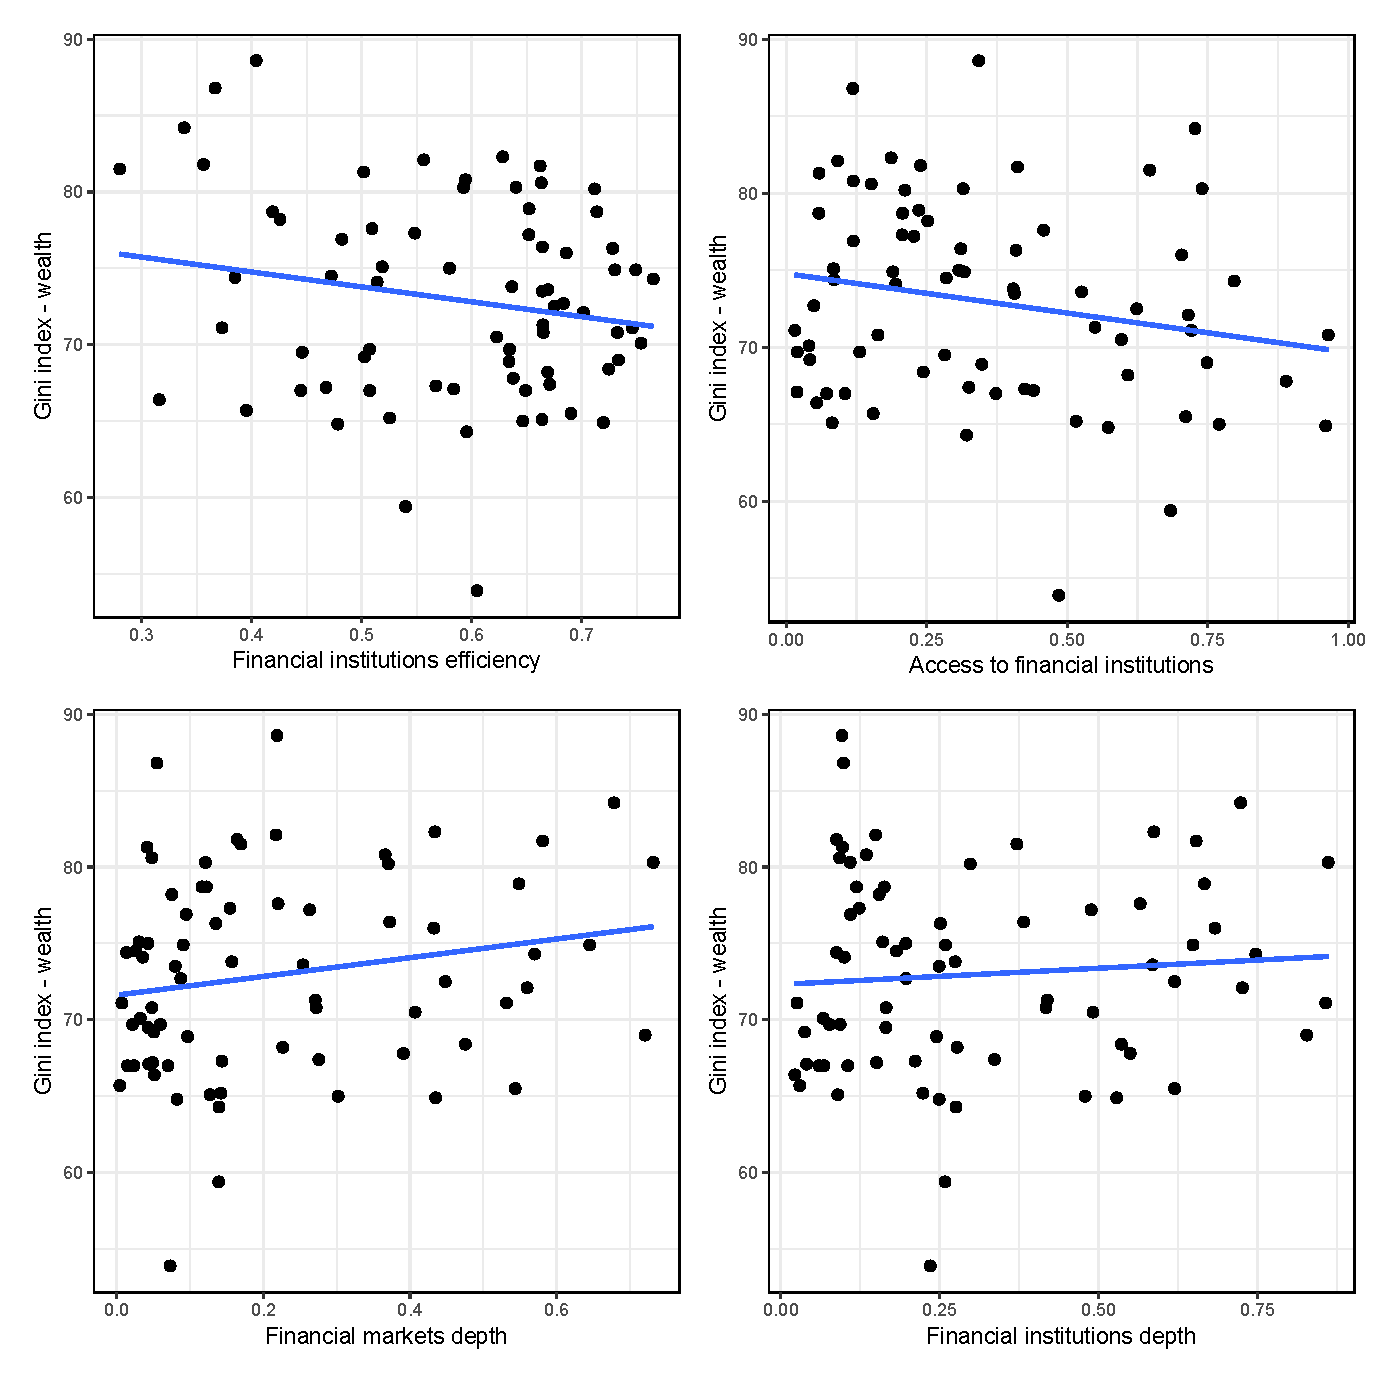
\includegraphics[width=0.85\textwidth, keepaspectratio]{figures/ch3/plots_findev.eps}
  \begin{minipage}{0.8\textwidth}
    \footnotesize
    \emph{Note:  Selected financial development indicators.}
    \end{minipage}
\end{figure}

Table \ref{ch3table:res1} presents our \ac{BMA} results regarding the determinants of wealth inequality. We present the explanatory variables sorted by their \ac{PIP} values and interpret the results in accordance with \textcite{kass1995bayes}, who present a conventional rule of thumb to evaluate the \ac{PIP}. When the \ac{PIP} is lower than 50\%, there is evidence against the effect, \ac{PIP} between 50\% and 75\% suggest a weak evidence for the effect, \ac{PIP} over 75\%, but less than 95\% means a “positive” evidence for the effect, in case of \ac{PIP} higher than 95\%, but less than 99\% there is strong evidence for the effect, and \ac{PIP} over 99\% provides decisive evidence for the effect.

According to our results, only a handful regressors robustly determines the cross-country variation in wealth inequality and exhibit \acp{PIP} greater than 0.5. Financial development indicators represent nearly half of these regressors, suggesting that finance is a crucial factor for understanding wealth inequality. Examining our global sample, our results suggest that cross-country differences in wealth inequality are a combination of effects stemming from finance, globalization, education, advances in agriculture and redistribution. But quantitatively, how important is this set of regressors in explaining wealth inequality? If we estimate the simple OLS regression with regressors included in the mode with the highest \ac{PMP}, we find the corresponding value of R-squared to be 0.57 (adjusted R-squared to be 0.52). This result suggests that we can explain approximately half of the variation in the cross-country differences in wealth inequality using only the eight most relevant regressors.\footnote{All regressors are statistically significant at the 1 or 10 percent level and exhibit signs of the coefficient estimates identical to those reported in Table \ref{ch3table:res1}. Alternatively, we estimate the model by OLS using the regressors with \acp{PIP} greater than 0.5 in the baseline \ac{BMA}. The results again correspond to the \ac{BMA} estimate. We report the output of both regressions in Table \ref{ch3res:ols} in the Appendix.} We discuss the effects of individual regressors in detail below.

The variables with high \acp{PIP} exhibit the expected qualitative effects on wealth distribution. The greater efficiency of financial intermediation and better access to the financial institutions results in a more uniform distribution of wealth. This finding is broadly in line with the conclusion of \textcite{claessens2007finance} regarding the determinants of income inequality, who assert that access to financial resources is a key driver in reducing income inequality rather than the depth of the financial market. The result of \textcite{claessens2007finance} also accords with the lower PIP of financial institutions depth in our model. 

According to our results, large financial markets (i.e., more capitalized stock markets and greater debt securities markets) propagate differences in wealth. Stock price booms are likely to increase wealth inequality because of the composition of household wealth, as stocks are typically owned by rich households. \textcite{kuhn} provide new estimates of wealth inequality in the US from 1949--2016 based on archival data from the Survey of Consumer Finances and examine the evolution of wealth over time. Their results are in accordance with ours: stock price booms indeed contribute to greater wealth inequality.  

In addition, one could argue that our result regarding the effect of the size of financial markets on wealth inequality corresponds to recent findings suggesting that too much finance is harmful to growth \parencite{Arcandetal2012,CecchettiKharroubi2012,LawSingh2014} and that it is important to disentangle quantity and quality of finance when examining the effect of finance on growth \parencite{hasan2016}. However, this analogy is only partially valid because whereas we typically think of greater economic performance as a positive phenomenon, there is a uncertainty about what is the `optimal' level of wealth inequality. 

Outward orientation capturing the openness of the economy leads to higher levels of wealth inequality. Large importance and qualitative effect correspond to the earlier findings, such as those of \textcite{dabla2015causes}, which claim that globalization and increasing exposure to the outside world contributes to greater within-country inequality. If globalization increases growth, then this result implies that the globalization benefits some economic agents more than others. For example, \textcite{dabla2015causes} and \textcite{milanovic2016global} mention the skill premium related to technological progress, which leads to excessive earnings and widens inequality. Nevertheless, our results provide little evidence that technological progress increases wealth inequality. We use a comprehensive index of technological progress developed by \textcite{comin}, but as we can observe from Table \ref{ch3table:res1}, its \ac{PIP} is very low. We attribute our result regarding the effect of technological progress on wealth inequality to the sample that we use. Our global sample covers countries with different degrees of economic development and technological progress, and it is likely that technological progress may play a greater role specifically in the most advanced countries. 

Redistribution, which we define as the difference between the market and after-tax income Gini indexes, contributes to lower wealth inequality. This result can be interpreted as evidence indicating that government policies may in fact affect inequality despite the well-known difficulties regarding the taxation of top earners. Our results are broadly in line with those of \textcite{jakobsen2018}, who find that the abolition of the Danish wealth tax in 1997 contributed to more wealth inequality by increasing the wealth of top earners. Interestingly, the political orientation of the government (as captured by the variable `left wing orientation') is not robustly related to wealth inequality. This result suggests that deeds (i.e., the actual level of redistribution) rather than words (i.e., stated political orientation) matter.\footnote{In one of the robustness checks, we also consider the relative redistribution (percentage reduction in market-income inequality due to taxes and transfers) Employing the alternative indicator of redistribution does not have any substantial impact on the other explanatory variables. The output of the estimation is available in Table \ref{ch3table:relred}.}.

Although the variable `number of war years' exhibits an inclusion probability of slightly less than 0.5, we find wars to be associated with higher wealth inequality. This result is at odds with previous evidence arguing that wars reduce inequality because of enormous capital destruction, inflation and sizable redistributive government programs (to finance the war); see, for example, \parencite{piketty2014,milanovic2016global} and the references therein. However, this evidence focuses on the effect of war on inequality over time and focuses on substantial and long-lasting conflicts, such as World War I or II. Our regressions explain cross-sectional variation in wealth inequality, i.e., why inequality is higher in some countries than in others. In addition, our dataset regarding wars is based on the period after World War II, i.e., typically internal conflicts (civil wars) or conflicts involving a single or small number of countries. These conflicts have adverse macroeconomic effects, undermine the rule of law, cause violent confiscation of private property by militias and reduce trust in society, especially if these conflicts occur repeatedly \parencite{bircanetal}. \textcite{bircanetal} study the effect of internal violent conflicts on income inequality and also find inequality increases, but this effect is temporary, and later on, inequality falls slowly back to the steady state.

\begin{table}[!ht]
\footnotesize
\centering
\caption{Determinants of Wealth Inequality, \ac{BMA} Estimation}
\label{ch3table:res1}
\begin{threeparttable}
\begin{tabular}{lrrr}
  \toprule
 & PIP & Post Mean & Post SD \\ 
    \midrule
  Financial institutions efficiency & 1.00 & -0.33651 & 0.11350 \\ 
  Value added in agriculture & 1.00 & -0.51800 & 0.16188 \\ 
  Access to financial institutions & 1.00 & -0.38266 & 0.15020 \\ 
  Outward orientation & 0.87 & 0.20663 & 0.12371 \\ 
  Education index (UN) & 0.79 & -0.26055 & 0.20440 \\ 
  Financial market development & 0.77 & 0.34023 & 0.23533 \\ 
  Redistribution & 0.51 & -0.10670 & 0.13963 \\ 
  Number of war years & 0.48 & 0.06956 & 0.09701 \\ 
  Net national savings & 0.42 & 0.08447 & 0.13021 \\ 
  Economic freedom index (adjusted) & 0.35 & -0.08233 & 0.15183 \\ 
  Financial institutions development & 0.33 & 0.14210 & 0.24598 \\ 
  Natural resource rents & 0.29 & 0.04572 & 0.09402 \\ 
  Net foreign direct investment & 0.25 & -0.03291 & 0.07552 \\ 
  Average GDP growth & 0.22 & -0.02607 & 0.06759 \\ 
  Labor market regulation & 0.16 & 0.01630 & 0.05386 \\ 
  Leftwing orientation & 0.15 & -0.01239 & 0.04533 \\ 
  Population density & 0.14 & -0.01540 & 0.05521 \\ 
  Inflation & 0.12 & 0.01036 & 0.04442 \\ 
  Government expenditures & 0.12 & 0.01311 & 0.05717 \\ 
  Latin America dummy & 0.10 & 0.00987 & 0.04762 \\ 
  Financial markets efficiency & 0.09 & -0.00706 & 0.04026 \\ 
  Banking diversification & 0.09 & -0.00579 & 0.03217 \\ 
  Rule of law & 0.09 & 0.01368 & 0.08087 \\ 
  Active banking restrictions & 0.09 & -0.00612 & 0.03667 \\ 
  Financial development index (EFW) & 0.07 & -0.00364 & 0.04464 \\ 
  Public education expenditures & 0.07 & 0.00363 & 0.02903 \\ 
  Revolutions and coups & 0.07 & 0.00250 & 0.02705 \\ 
  Population growth & 0.07 & 0.00394 & 0.04154 \\ 
  Bank capital regulations & 0.07 & -0.00323 & 0.02589 \\ 
  GDP level in 1990 & 0.07 & -0.00809 & 0.07483 \\ 
  Civ. liberties and pol. rights & 0.06 & -0.00322 & 0.04104 \\ 
  Technological progress & 0.06 & -0.00596 & 0.06110 \\ 
  Life expectancy & 0.05 & 0.00043 & 0.04581 \\ 
  Financial openness (Chinn-Ito) & 0.05 & 0.00150 & 0.03218 \\ 
  Business conditions & 0.05 & -0.00196 & 0.02568 \\ 
  Value added in industry & 0.05 & -0.00030 & 0.02710 \\ 
  Labor force participation & 0.04 & 0.00054 & 0.01815 \\ 
  \midrule
  \bottomrule
\end{tabular}
\begin{tablenotes}
\item 
\footnotesize
\textit{Note: Dependent variable - average Gini index (wealth) 2010-2016, 73 observations, baseline (hyper-g parameter prior)}
\end{tablenotes}
\end{threeparttable}
\end{table}

\clearpage
\begin{figure}
	\caption{Robustness Check: Different Prior Structure}
	\centering
	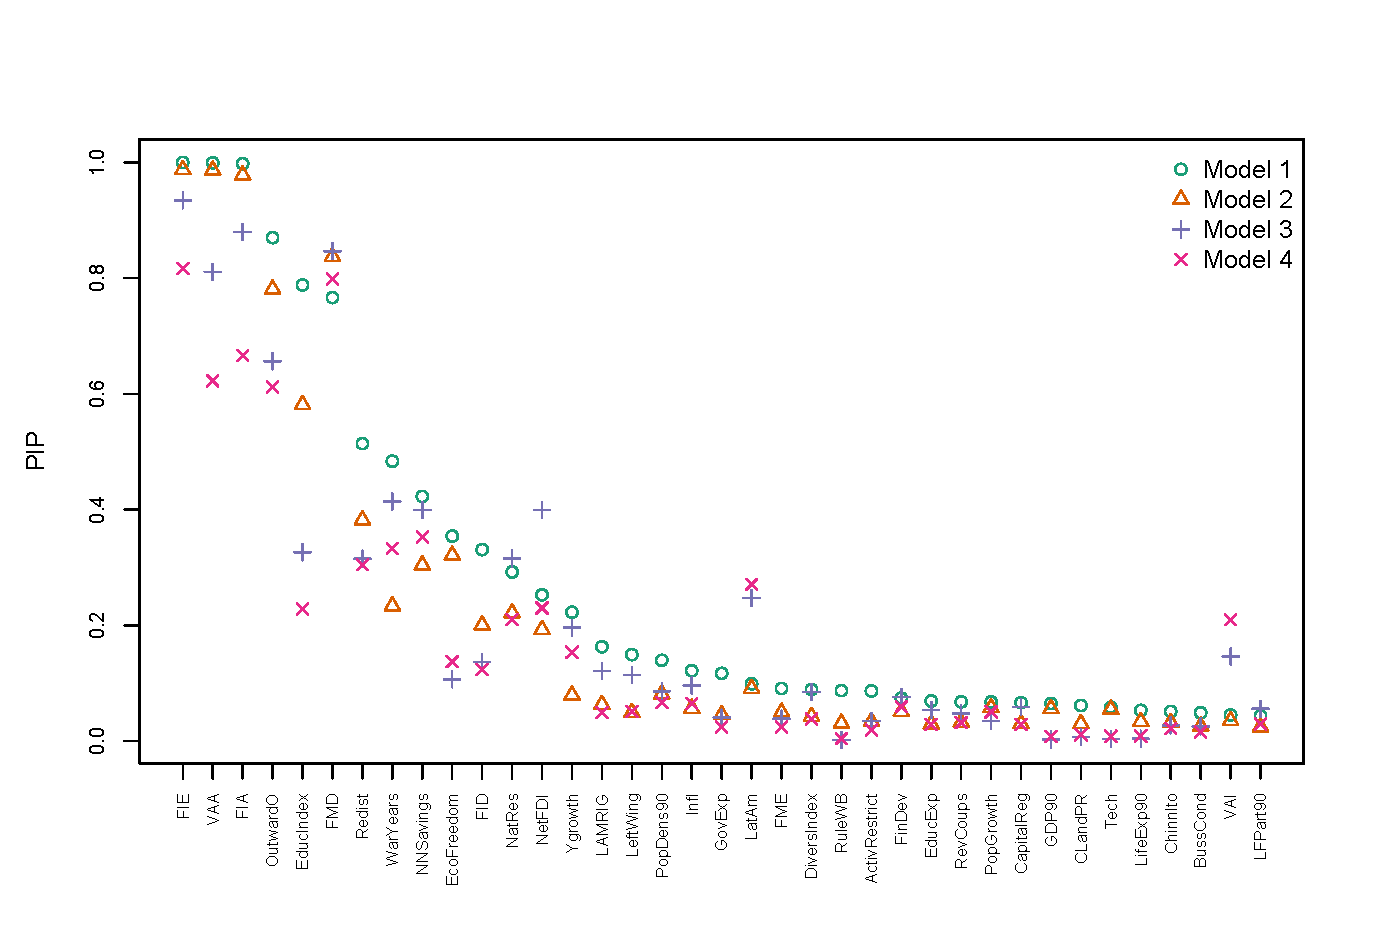
\includegraphics[width=0.9\textwidth]{figures/ch3/priors_comparison_compound.eps}
  \label{ch3fig:comp_compound}
  \begin{minipage}{0.8\textwidth}
    \footnotesize
    \emph{Note: Parameter and model prior comparison - compound indicators. Model 1: hyper-g, uniform; Model 2: \ac{UIP}, uniform; Model 3: hyper-g, dilution; Model 4: \ac{UIP}, dilution.}
  \end{minipage}
\end{figure}

We report the baseline results, in which we employ the uniform model prior and hyper-g parameter prior, as described in section \ref{ch3sec:BMA}. To provide robustness checks, we also use alternative parameter and model priors. Figure \ref{ch3fig:comp_compound} presents a graphical illustration of our robustness checks. We estimate alternative specifications of the model using \ac{UIP} and the dilution model prior described earlier. Overall, the results are similar. The optional priors slightly decrease \ac{PIP} across the set of regressors, with the combined effect of \ac{UIP} and dilution model prior having the largest effect. This slight overall decrease in inclusion probabilities is related to the smaller models dictated by the alternative prior structures, but the ordering of the variables in terms of \ac{PIP} remains quite stable. The only exception to marginal decreases in the \ac{PIP} is the effect of education, which decreases to less than 0.5 when we apply the dilution model prior in the estimation. This result could be partially explained by the design of this particular prior, which should down-weight variables that are highly correlated with others. We also tried other specifications with quadratic terms of financial indexes, interactions between the rule of law and financial indexes, and others.\footnote{For example, we investigate cases where we drop groups of variables as defined in Table \ref{ch3tab:groups}. Interestingly, when we drop a group of low \ac{PIP} variables, the results are stable. On the other hand, if we drop a group which contains variables with high \acp{PIP}, the results deviate from the baseline estimates. This could be due to the introduction of omitted variable bias in the latter case as dropping important regressors may severely affect coefficients on the remaining variables.} None of these additional regressors exhibited significant relevance in our model.\footnote{These additional estimation results are available upon request.}

Next, we argue that the effect of finance on wealth inequality is complex and whereas some financial indicators decrease the inequality, other financial indicators increase it. But what is the overall effect of finance on wealth inequality? We take the estimated posterior means from Table \ref{ch3table:res1} for the finance variables with \ac{PIP} values greater than 0.5 (these are access to financial institutions (FIA), their efficiency (FIE), and the depth of stock market (FMD)) and multiply them by the corresponding country-specific values. Given the manner in which our explanatory variables are normalized, this multiplication is identical to examining the change in wealth inequality as a result of one-standard-deviation increases in FIA, FIE, and FMD. 

We present the results of overall effect of finance on wealth inequality in Figure \ref{ch3fig:finance_effect}. Even though we do not want to overemphasize the precision of our results, the estimated effect is negative for all countries in our sample, i.e., our results suggest that greater financial development reduces wealth inequality. Nevertheless, we observe some heterogeneity in the estimated effect across the countries. Interestingly, we observe the weakest decreasing effect of finance on wealth inequality for the \ac{US}.\footnote{Alternatively, we assessed the overall effect of finance on wealth inequality based on the estimation of the \ac{OLS} model. We selected the explanatory variables that had \ac{PIP} values in \ref{ch3table:res1} greater than 0.5. The results are largely the same and are available upon request.}

\begin{sidewaysfigure}
\begin{center}
\caption{Effects of individual financial development components on inequality}
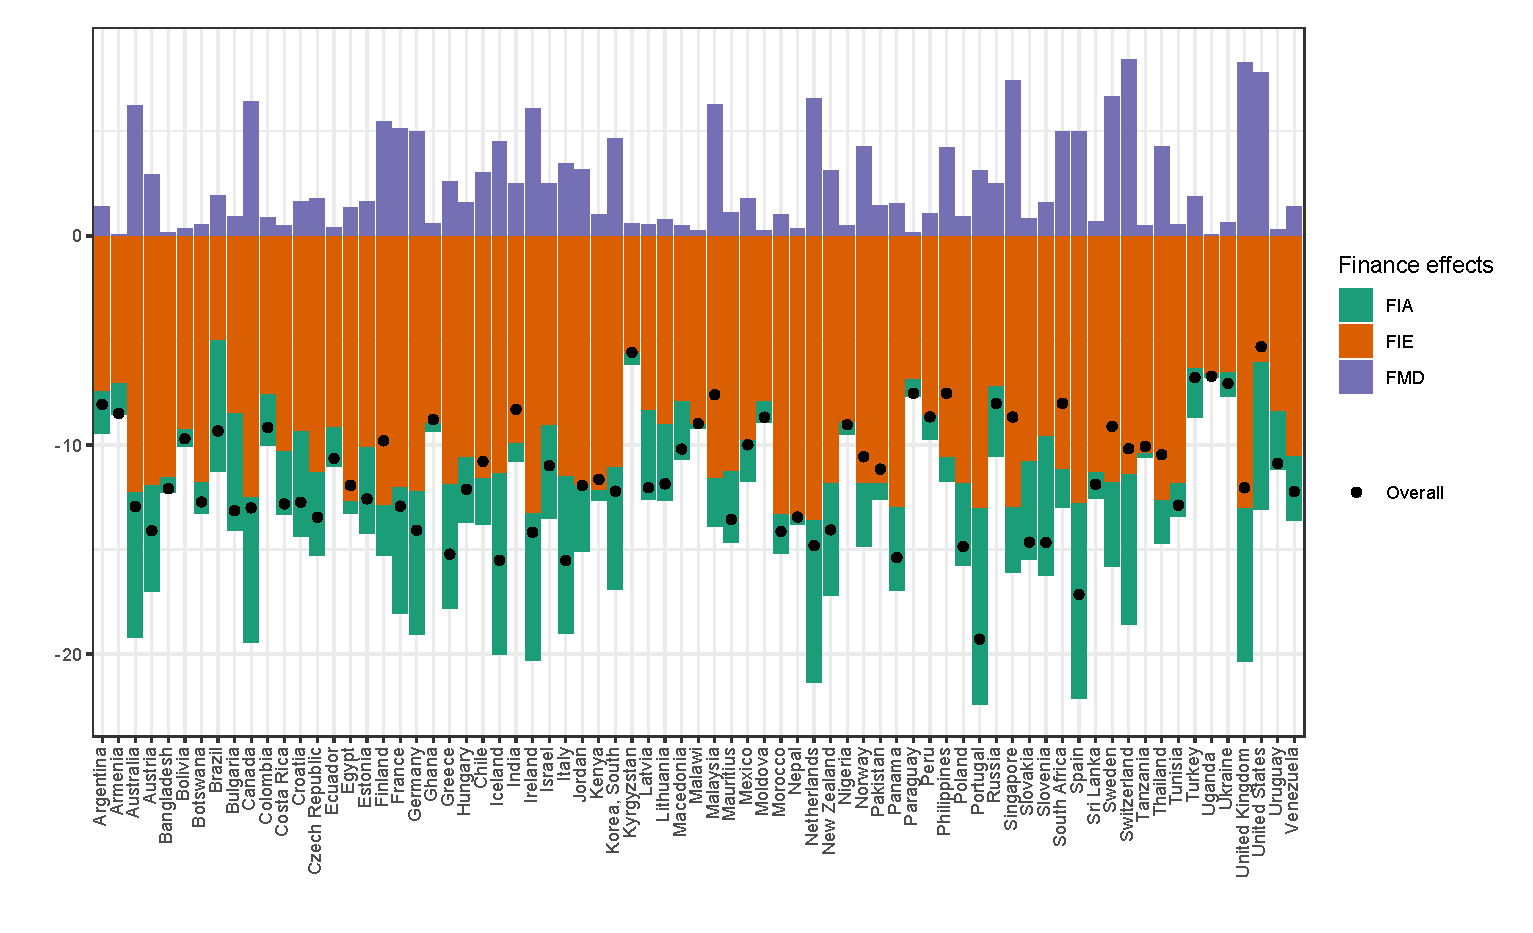
\includegraphics[width=0.95\textwidth]{figures/ch3/finance_effect.eps}
\label{ch3fig:finance_effect}
\end{center}
\end{sidewaysfigure}

\subsection{High vs. low-income countries}
We explore the non-linearity of the estimated effects by splitting our sample into two halves according to the level of GDP in 1990. Such an exercise, however, presents an issue for the estimation with the full set of explanatory variables as only 36 observations remain in each sample. To overcome this, we consider nine explanatory variables which occur in the top three models by their \ac{PMP} which gives us enough degrees of freedom for the estimation. 

We present the results in Table \ref{ch3tab:inc_comparison}. The estimated coefficients of explanatory variables have their expected signs. We observe some heterogeneity in terms of \acp{PIP}. We find that technological advancement in agriculture (value added in agriculture) and openness of the economy (outward orientation) are dominant factors for low-income countries, while they are less relevant for the group of high-income countries. This is expected result given the prominence of agriculture sector in developing countries. Wars matter both for low-income and high-income countries. Regarding the financial variables, depth of the financial market increases wealth inequality both in low-income and high-income countries. Other financial variables (access to finance and efficiency of financial intermediaries) reduce wealth inequality especially in high-income countries. This suggests that the role of finance for wealth inequality rises with economic development.  

\begin{table}[htbp!]
\caption{Estimates using the variables from the model with the highest posterior model probability and sample split into high- / low- income countries (based on GDP90)}
\label{ch3tab:inc_comparison}
\centering
\begin{tabular}{lrrrr}
  \toprule
  & \multicolumn{2}{c}{High-income} & \multicolumn{2}{c}{Low-income} \\
  \midrule
	 & \ac{PIP} & Post. Mean & \ac{PIP} & Post. Mean \\ 
  \midrule
  Financial market depth & 0.97 & 0.55171 & 0.66 & 0.21279 \\ 
  Average GDP growth & 0.83 & -0.31499 & 0.23 & 0.00877 \\ 
  Access to FI & 0.76 & -0.30279 & 0.27 & 0.04851 \\ 
  Number of war years & 0.72 & 0.36526 & 0.62 & 0.09226 \\ 
  FI efficiency & 0.60 & -0.22569 & 0.24 & -0.00668 \\ 
  Redistribution & 0.56 & -0.16593 & 0.27 & -0.02704 \\ 
  Outward orientation & 0.50 & 0.11034 & 1.00 & 0.36512 \\ 
  Education index (UN) & 0.38 & -0.10648 & 0.32 & -0.04479 \\ 
  Value added in agriculture & 0.29 & 0.03537 & 0.94 & -0.33730 \\ 
   \bottomrule
\end{tabular}
\end{table}

\subsection{Endogeneity issues}
In our baseline results, we address endogeneity issues by estimating the effect of lagged regressors on wealth inequality. While wealth inequality is based on the data between 2010-2016, the regressors are based on data prior 2010 and often cover the 1980s, 1990s or 2000s. Therefore, we followed the procedure typical for \ac{BMA} literature \parencite{christofides,feldkircherjimf,hasan2016}.  

The question of endogeneity is, however, deeply ingrained in the finance-inequality nexus, and we want to provide additional evidence that the estimated effect of finance on wealth distribution is causal. There are reasons for caution. First, a wealth distribution that is more concentrated at the top may result in more power of incumbents, who lobby for funding of their projects using their political connections and thereby distort the market. Second, making the distribution of wealth more equal may lead to increased demand for financial services as more individuals seek to invest their savings or take up loans when their wealth provides a satisfactory collateral. If such development leads to increased supply of financial services through, for example, newly installed ATMs and opened institutions, it may manifest as better access to financial services \parencite{beck2007finance}.

To address the potential endogeneity of the relationship between wealth distribution and financial development, we apply \ac{IVBMA}. This methodology suggested by \textcite{KarlLenkoski2012} implements the idea of instrumental variables in a Bayesian framework. It is essentially a two-stage estimation in which model uncertainty is considered in both stages. In the robustness check, we set the depth of financial institutions and access to financial institutions endogenous, as we believe that from our set of financial indicators, these are most the ones most likely affected by the reverse causality issues presented previously.

We employ genetic distance from the United States \parencite{spolaore2009diffusion} along with a measure of financial liberalization as instruments. The financial liberalization proxy we construct relies on the components of \ac{EFW} index by \parencite{gwartney2017}. More specifically, we average the areas 3D, 4C, 4D, and 5A of the \ac{EFW}. These represent freedom to own foreign currency accounts, black-market exchange rate premium, controls on the movement of capital and people, and credit market regulations. We refer to the authors of \ac{EFW} for the details of individual components. Although the search for good instruments is a nontrivial exercise, we believe our choice satisfies the basic conditions. Genetic distance should be unrelated to wealth distribution\footnote{In our sample, the correlation is 0.06.}. Even if the primary cause of migration is more/less equal distribution of wealth, it would most likely not be sufficiently substantial to affect the genetic pattern in a particular country. Additionally, the components of our financial liberalization measure are exogenous to the wealth inequality as the change in wealth distribution is improbably to have direct effect on any of them. We follow \textcite{estev} here, who treat foreign trade liberalization as exogenous.

We check the strength of our instruments by examining the correlations and running simple \ac{OLS} regressions of our endogenous variable on the instruments. The correlations of the instruments are greater than 0.5 in absolute terms, with the only exception being FID and genetic distance, for which it is -0.37. The regressions reveal strong significance of the instruments and the F-test statistics of the regressions are 35.43 and 19.95 for FIA and FID, respectively. Both values are well above 10, the rule of thumb proposed by \textcite{staiger1997instrumental}. We have compared several additional instruments often used in the literature, including the ubiquitously used financial reform index by \textcite{Abiadetal2008} and the legal origin of the countries, but the \ac{EFW} measure turned out to be the strongest of the instruments. Our main \ac{IVBMA} results rely on the just-identified case where we have two potential instruments for two potentially endogenous variables. We check the overidentification with Sargan test as introduced in \textcite{lenkoski2014two}, where the Sargan p-value is an weighted average of p-values from individual combinations of first and second stage models weighted by their model probabilities. The values are only available for potentially overidentified cases, where the number of instruments considered in the first stage is higher than the number of assumed endogenous variables. The averaged p-value from these cases confirms the validity of instruments.

Table \ref{ch3table:res_endo} presents the results of the \ac{IVBMA} estimation. The \acp{PIP} of instrumented variables somewhat decrease, in the case of access to financial institutions slightly below 0.5, but it still remains among the most important regressors. We also confirm the positive effect of financial markets depth along with the high inclusion probability. The \acp{PIP} cannot be directly compared with the baseline results due to differences in the estimation procedure. Whereas for the standard \ac{BMA} we report the inclusion probabilities based on the analytical posterior probabilities of the top models, \ac{IVBMA} reports the probabilities based on the sampler. The latter approach tends to downweigh the \ac{PIP} for the top and upweight it for the bottom regressors.\footnote{If we compare \ac{IVBMA} output with the MC$^3$ \acp{PIP} from the baseline \ac{BMA}, we obtain very similar values for both approaches.} Overall, the \ac{IVBMA} estimation largely supports our baseline findings. 

\begin{table}[!ht]
	\footnotesize
	\centering
	\caption{Determinants of Wealth Inequality, \ac{IVBMA} Estimation}
	\label{ch3table:res_endo}
	\begin{threeparttable}
	\begin{tabular}{lrrr}
		\toprule
		& \ac{PIP} & Post. Mean & Post. SD\\ 
		\midrule
		Financial institutions efficiency & 0.85826 & -0.32431 & 0.18276 \\ 
		Value added in agriculture & 0.78741 & -0.39918 & 0.27546 \\ 
		Financial market depth & 0.62200 & 0.29196 & 0.32026 \\ 
		Financial institutions depth & 0.55682 & 0.24718 & 0.39989 \\ 
		Outward orientation & 0.52022 & 0.13647 & 0.15901 \\ 
		Economic freedom index (adjusted) & 0.50242 & -0.18778 & 0.24043 \\ 
		Education index (UN) & 0.46915 & -0.16719 & 0.23034 \\ 
		Access to financial institutions & 0.45168 & -0.19051 & 0.31849 \\ 
		Net national savings & 0.42093 & 0.11213 & 0.16687 \\ 
		Redistribution & 0.39198 & -0.10184 & 0.15932 \\ 
		Natural resource rents & 0.36756 & 0.08280 & 0.13856 \\ 
		Number of war years & 0.36660 & 0.07267 & 0.11648 \\ 
		GDP level in 1990 & 0.29348 & -0.03476 & 0.21811 \\ 
		Latin America dummy & 0.25851 & 0.05039 & 0.11744 \\ 
		Net foreign direct investment & 0.24740 & -0.04159 & 0.09389 \\ 
		Technological progress & 0.24198 & -0.02756 & 0.15284 \\ 
		Rule of law & 0.22111 & 0.00025 & 0.13277 \\ 
		Life expectancy & 0.21608 & -0.02082 & 0.12509 \\ 
		Value added in industry & 0.20523 & 0.03081 & 0.09693 \\ 
		Civ. liberties and pol. rights & 0.17607 & 0.00152 & 0.08731 \\ 
		Population growth & 0.17297 & 0.01557 & 0.08178 \\ 
		Inflation & 0.17219 & 0.02180 & 0.07214 \\ 
		Average GDP growth & 0.16884 & -0.01947 & 0.06804 \\ 
		Population density & 0.15698 & -0.01672 & 0.06680 \\ 
		Government expenditures & 0.15095 & 0.01087 & 0.06574 \\ 
		Labor market regulation & 0.14337 & 0.01307 & 0.05424 \\ 
		Financial openness (Chinn-Ito) & 0.13893 & -0.00881 & 0.06817 \\ 
		Leftwing orientation & 0.13809 & -0.01337 & 0.04972 \\ 
		Business conditions & 0.12686 & -0.00665 & 0.05531 \\ 
		Financial markets efficiency & 0.12605 & -0.00358 & 0.05153 \\ 
		Revolutions and coups & 0.12206 & 0.00728 & 0.04631 \\ 
		Active banking restrictions & 0.11903 & -0.00620 & 0.04858 \\ 
		Banking diversification & 0.11722 & -0.00860 & 0.04230 \\ 
		Public education expenditures & 0.10759 & 0.00368 & 0.03795 \\ 
		Bank capital regulations & 0.09251 & -0.00155 & 0.03023 \\ 
		Labor force participation & 0.09011 & -0.00148 & 0.02810 \\ 
		\bottomrule
	\end{tabular}
\begin{tablenotes}
\footnotesize
\item \textit{Note: Dependent variable - average Gini index (wealth) 2010-2016, 73 observations. Financial depth of and access to financial institutions as endogenous. Instruments: genetic distance, financial development index from Economic Freedom of the World.}
\end{tablenotes}
\end{threeparttable}
\end{table}
%
%
%
%
%
\section{Concluding Remarks}
\label{ch3sec:conclusion}

This paper makes a new contribution to the burgeoning literature about wealth inequality. Whereas the existing literature focuses largely on measurement of wealth inequality \parencite{alvaredoetal2013,daviesetal2011,pikettyandzucman2014,SaezZucman2016}, we examine a wide array of possible determinants of wealth inequality. 

Building the large cross-country dataset, we employ \ac{BMA} to study the determinants of wealth inequality in order to address the regression model uncertainty. This uncertainty arises from the lack of an encompassing model of wealth inequality, which would dictate the exact regression specification to be estimated. As a side effect, using \ac{BMA}, we can examine a large number of possible determinants of wealth inequality within a unifying framework. Therefore, we examine how different economic, financial, regulatory, political, social, and institutional variables affect wealth inequality.  

Using our global sample, addressing endogeneity issues and subjecting our results to a number of robustness checks, we find that only a handful variables are robustly related to wealth inequality. Our results suggest that cross-country differences in wealth inequality arise due to a combination of the effects stemming from the financial sector, globalization, education, advances in agriculture and government redistribution. More specifically, our baseline estimation shows that there are seven regressors with PIP values greater than 50\%, and they explain approximately half of the cross-country differences in wealth inequality. 

We find that finance plays an important role in wealth inequality. Out of seven aforementioned variables that are robustly related to wealth inequality, three of them capture the level of financial development. According to our results, finance exerts a complex effect on wealth inequality. Some financial characteristics increase inequality, whereas other financial characteristics, to the contrary, decrease it.

Our results show that large financial markets (as proxied by the stock market capitalization and size of debt securities market type of variables) are associated with greater wealth inequality. This result follows from the composition effect, as it is typically rich households that participate in the stock markets \parencite{kuhn}. On the other hand, our findings show that countries with better access to finance and more efficient financial intermediaries exhibit lower wealth inequality. Therefore, there is no natural tendency that financial development results into greater wealth inequality. On the contrary, when we take the average values of financial development measures, the overall effect of finance development on wealth inequality is negative (i.e., more financially developed countries associated with lower level of wealth inequality). 

In addition, our results show that more education and greater income redistribution are associated with lower level of wealth inequality. Therefore, this result broadly suggest that governments can affect the inequality within their countries (either via education or taxation). In addition, we also find that (the lack of) political stability influences wealth inequality, as our results show that countries with war experience exhibit greater inequality. Finally, our results suggest that globalization but not technological development is likely to contribute to greater wealth inequality.
%
%
%
%
\newpage
% \fancyhead[LO]{\sffamily Bibliography}		%headers in sans serif and not in uppercase
% \bibliographystyle{Styles/Stylebib}			%style of literature, you can use e.g. newapa	instead of Styles/Stylebib
% \bibliography{Styles/literature}
\printbibliography[heading=subbibliography]
\addcontentsline{toc}{section}{References}
%
%
\newpage
\section*{Appendix}
\begin{subappendices}
    \section{Additional robustness checks}
    \label{ch3sec:app_rch}
    \begin{table}[!ht]
    \footnotesize
    \centering
    \caption{Dependent variable - average Gini index (wealth) 2010-2016, 73 observations, \ac{UIP} parameter prior}
    \label{ch3table:res2}
    \begin{tabular}{lrrr}
      \toprule
     & \ac{PIP} & Post Mean & Post SD \\ 
      \midrule
      Financial institutions efficiency & 0.99 & -0.36999 & 0.12386 \\ 
      Value added in agriculture & 0.99 & -0.56485 & 0.18154 \\ 
      Access to financial institutions & 0.98 & -0.44382 & 0.16204 \\ 
      Financial market development & 0.84 & 0.44193 & 0.23922 \\ 
      Outward orientation & 0.78 & 0.21853 & 0.14535 \\ 
      Education index (UN) & 0.58 & -0.23984 & 0.24290 \\ 
      Redistribution & 0.38 & -0.10095 & 0.15101 \\ 
      Economic freedom index (adjusted) & 0.32 & -0.10501 & 0.18144 \\ 
      Net national savings & 0.30 & 0.07686 & 0.13764 \\ 
      Number of war years & 0.23 & 0.03833 & 0.08335 \\ 
      Natural resource rents & 0.22 & 0.04549 & 0.10083 \\ 
      Financial institutions development & 0.20 & 0.10354 & 0.23661 \\ 
      Net foreign direct investment & 0.19 & -0.03276 & 0.08044 \\ 
      Latin America dummy & 0.09 & 0.01404 & 0.05849 \\ 
      Population density & 0.08 & -0.01162 & 0.05108 \\ 
      Average GDP growth & 0.08 & -0.00950 & 0.04338 \\ 
      Labor market regulation & 0.06 & 0.00671 & 0.03585 \\ 
      Population growth & 0.06 & 0.00788 & 0.04715 \\ 
      Inflation & 0.06 & 0.00568 & 0.03341 \\ 
      GDP level in 1990 & 0.06 & -0.01404 & 0.08467 \\ 
      Technological progress & 0.05 & -0.01188 & 0.07248 \\ 
      Financial development index (EFW) & 0.05 & -0.00641 & 0.04430 \\ 
      Financial markets efficiency & 0.05 & -0.00499 & 0.03332 \\ 
      Leftwing orientation & 0.05 & -0.00400 & 0.02612 \\ 
      Government expenditures & 0.05 & 0.00463 & 0.03646 \\ 
      Banking diversification & 0.04 & -0.00316 & 0.02370 \\ 
      Value added in industry & 0.04 & 0.00229 & 0.03279 \\ 
      Life expectancy & 0.03 & -0.00160 & 0.03867 \\ 
      Active banking restrictions & 0.03 & -0.00213 & 0.02262 \\ 
      Revolutions and coups & 0.03 & 0.00178 & 0.02012 \\ 
      Financial openness (Chinn-Ito) & 0.03 & -0.00137 & 0.02553 \\ 
      Rule of law & 0.03 & 0.00093 & 0.03789 \\ 
      Civ. liberties and pol. rights & 0.03 & -0.00131 & 0.02953 \\ 
      Bank capital regulations & 0.03 & -0.00131 & 0.01725 \\ 
      Public education expenditures & 0.03 & 0.00113 & 0.01817 \\ 
      Business conditions & 0.03 & -0.00000 & 0.01732 \\ 
      Labor force participation & 0.02 & 0.00028 & 0.01376 \\  
      \bottomrule
    \end{tabular}
    \end{table}
    
    \clearpage
    
    \begin{table}[!ht]
    \footnotesize
    \centering
    \caption{Dependent variable - average Gini index (wealth) 2010-2016, 73 observations, dilution parameter prior}
    \label{ch3table:res3}
    \begin{tabular}{lrrr}
      \toprule
     & \ac{PIP} & Post Mean & Post SD \\ 
      \midrule
      Financial institutions efficiency & 0.93 & -0.29559 & 0.14058 \\ 
      Access to financial institutions & 0.88 & -0.35265 & 0.19165 \\ 
      Financial market development & 0.85 & 0.38321 & 0.21129 \\ 
      Value added in agriculture & 0.81 & -0.37066 & 0.23301 \\ 
      Outward orientation & 0.66 & 0.15971 & 0.14225 \\ 
      Number of war years & 0.41 & 0.06813 & 0.10412 \\ 
      Net national savings & 0.40 & 0.10489 & 0.15200 \\ 
      Net foreign direct investment & 0.40 & -0.06582 & 0.10158 \\ 
      Education index (UN) & 0.33 & -0.12682 & 0.20519 \\ 
      Natural resource rents & 0.32 & 0.06267 & 0.11045 \\ 
      Redistribution & 0.32 & -0.08372 & 0.14239 \\ 
      Latin America dummy & 0.25 & 0.04844 & 0.10292 \\ 
      Average GDP growth & 0.20 & -0.02656 & 0.07126 \\ 
      Value added in industry & 0.15 & 0.03229 & 0.09069 \\ 
      Financial institutions development & 0.14 & 0.06411 & 0.17325 \\ 
      Labor market regulation & 0.12 & 0.01228 & 0.04752 \\ 
      Leftwing orientation & 0.11 & -0.00800 & 0.03714 \\ 
      Economic freedom index (adjusted) & 0.11 & -0.03180 & 0.10542 \\ 
      Inflation & 0.10 & 0.01006 & 0.04385 \\ 
      Population density & 0.09 & -0.00999 & 0.04676 \\ 
      Banking diversification & 0.09 & -0.00557 & 0.03201 \\ 
      Financial development index (EFW) & 0.08 & -0.01339 & 0.05852 \\ 
      Bank capital regulations & 0.06 & -0.00114 & 0.02308 \\ 
      Labor force participation & 0.06 & -0.00002 & 0.02089 \\ 
      Public education expenditures & 0.05 & 0.00208 & 0.02499 \\ 
      Revolutions and coups & 0.05 & 0.00270 & 0.02436 \\ 
      Government expenditures & 0.04 & 0.00506 & 0.03702 \\ 
      Financial markets efficiency & 0.04 & -0.00350 & 0.02844 \\ 
      Population growth & 0.04 & 0.00542 & 0.04010 \\ 
      Active banking restrictions & 0.03 & -0.00191 & 0.02272 \\ 
      Financial openness (Chinn-Ito) & 0.03 & -0.00266 & 0.02558 \\ 
      Business conditions & 0.03 & 0.00043 & 0.01735 \\ 
      Civ. liberties and pol. rights & 0.01 & 0.00054 & 0.01473 \\ 
      Life expectancy & 0.00 & -0.00069 & 0.01508 \\ 
      Technological progress & 0.00 & -0.00099 & 0.02030 \\ 
      GDP level in 1990 & 0.00 & -0.00102 & 0.02294 \\ 
      Rule of law & 0.00 & -0.00013 & 0.00744 \\
      \bottomrule
    \end{tabular}
    \end{table}
    
    \clearpage
    
    \begin{table}[!ht]
    \footnotesize
    \centering
    \caption{Dependent variable - average Gini index (wealth) 2010-2016, 73 observations, relative redistribution measure}
    \label{ch3table:relred}
    \begin{tabular}{lrrr}
      \toprule
     & \ac{PIP} & Post Mean & Post SD \\ 
      \midrule
      Value added in agriculture & 1.00 & -0.51152 & 0.15591 \\ 
      Financial institutions efficiency & 0.99 & -0.28741 & 0.11147 \\ 
      Access to financial institutions & 0.98 & -0.34837 & 0.15459 \\ 
      Redistribution (rel.) & 0.95 & -0.27535 & 0.14043 \\ 
      Outward orientation & 0.94 & 0.23308 & 0.11250 \\ 
      Financial market depth & 0.81 & 0.34002 & 0.21938 \\ 
      Education index (UN) & 0.72 & -0.22528 & 0.20282 \\ 
      Number of war years & 0.59 & 0.08973 & 0.10332 \\ 
      Economic freedom index (adjusted) & 0.36 & -0.08389 & 0.15606 \\ 
      Labour market regulation & 0.32 & 0.03829 & 0.07734 \\ 
      Natural resources rents & 0.28 & 0.04065 & 0.08833 \\ 
      Financial institutions depth & 0.28 & 0.10702 & 0.21832 \\ 
      Average GDP growth & 0.28 & -0.03598 & 0.07976 \\ 
      Rule of law & 0.26 & 0.07442 & 0.17734 \\ 
      Leftwing orientation & 0.22 & -0.02359 & 0.06261 \\ 
      Net foreign direct investment & 0.20 & -0.02042 & 0.05956 \\ 
      Net national savings & 0.20 & 0.02747 & 0.08091 \\ 
      Government expenditures & 0.16 & 0.01994 & 0.06646 \\ 
      Bank capital regulations & 0.11 & -0.00826 & 0.03810 \\ 
      Population density & 0.10 & -0.00737 & 0.03893 \\ 
      Civ. liberties and Pol. rights & 0.09 & -0.00684 & 0.05487 \\ 
      Business conditions & 0.09 & -0.00679 & 0.03889 \\ 
      GDP level in 1990 & 0.09 & -0.00754 & 0.08113 \\ 
      Public education expenditures & 0.09 & 0.00452 & 0.03209 \\ 
      Financial openness (Chinn-Ito) & 0.08 & 0.00371 & 0.04077 \\ 
      Banking diversification & 0.08 & -0.00453 & 0.02891 \\ 
      Financial liberalization (EFW) & 0.08 & -0.00225 & 0.04299 \\ 
      Active banking restrictions & 0.08 & -0.00396 & 0.03201 \\ 
      Latin America dummy & 0.07 & 0.00613 & 0.08853 \\ 
      Technological progress & 0.07 & -0.00810 & 0.06770 \\ 
      Financial markets efficiency & 0.06 & -0.00027 & 0.03059 \\ 
      Inflation & 0.06 & 0.00238 & 0.02706 \\ 
      Labour force participation & 0.06 & 0.00036 & 0.02077 \\ 
      Life expectancy & 0.06 & 0.00055 & 0.04579 \\ 
      Population growth & 0.06 & 0.00076 & 0.03609 \\ 
      Value added in industry & 0.05 & -0.00063 & 0.02761 \\ 
      Revolutions and coups & 0.05 & 0.00069 & 0.02121 \\ 
       \bottomrule
    \end{tabular}
    \end{table}
    
    \clearpage
    
    \begin{table}[!ht]
    \footnotesize
    \centering
    \caption{Dependent variable - average Gini index (wealth) 2010-2016, specific financial indicators as proxies for financial development, 73 observations, dilution parameter prior}
    \label{ch3table:res5}
    \begin{tabular}{lrrr}
      \toprule
     & \ac{PIP} & Post Mean & Post SD \\ 
      \midrule
      Outward orientation & 1.00 & 0.30288 & 0.09493 \\ 
      Value added in agriculture & 1.00 & -0.46969 & 0.16524 \\ 
      Number of war years & 1.00 & 0.23140 & 0.09211 \\ 
      Bank branches/1000 inh. & 0.99 & -0.23286 & 0.10392 \\ 
      Redistribution & 0.96 & -0.27204 & 0.13368 \\ 
      Private credit & 0.80 & 0.26709 & 0.20234 \\ 
      Average GDP growth & 0.72 & -0.12719 & 0.11806 \\ 
      Net interest margin & 0.71 & 0.26047 & 0.23046 \\ 
      Business conditions & 0.63 & -0.16526 & 0.17583 \\ 
      Inflation & 0.52 & 0.08140 & 0.10963 \\ 
      Education index (UN) & 0.43 & -0.09997 & 0.16364 \\ 
      Economic freedom index (adjusted) & 0.38 & -0.11007 & 0.18830 \\ 
      Leftwing orientation & 0.26 & -0.02542 & 0.06428 \\ 
      Labor market regulation & 0.17 & 0.01351 & 0.04931 \\ 
      Rule of law & 0.17 & 0.02859 & 0.11191 \\ 
      Net national savings & 0.16 & 0.01665 & 0.06290 \\ 
      Natural resource rents & 0.16 & 0.01609 & 0.06250 \\ 
      Bank Z-score & 0.15 & 0.01193 & 0.04857 \\ 
      Latin America dummy & 0.13 & 0.01040 & 0.05422 \\ 
      Banking diversification & 0.12 & -0.00670 & 0.03591 \\ 
      Market capitalization & 0.11 & 0.00106 & 0.04334 \\ 
      Market turnover & 0.11 & 0.00559 & 0.03372 \\ 
      Civ. liberties and pol. rights & 0.11 & 0.00419 & 0.05246 \\ 
      Value added in industry & 0.11 & 0.00610 & 0.04528 \\ 
      Population growth & 0.11 & 0.00659 & 0.05385 \\ 
      Life expectancy & 0.10 & -0.00578 & 0.06521 \\ 
      Technological progress & 0.10 & 0.00530 & 0.08492 \\ 
      Financial development index (EFW) & 0.10 & 0.00203 & 0.05079 \\ 
      Net foreign direct investment & 0.10 & -0.00504 & 0.03344 \\ 
      GDP level in 1990 & 0.10 & 0.00277 & 0.08595 \\ 
      Financial openness (Chinn-Ito) & 0.09 & 0.00422 & 0.04314 \\ 
      Public education expenditures & 0.09 & 0.00437 & 0.03492 \\ 
      Government expenditures & 0.09 & 0.00648 & 0.04413 \\ 
      Loan-to-deposits & 0.09 & 0.00400 & 0.03650 \\ 
      Revolutions and coups & 0.09 & 0.00307 & 0.03130 \\ 
      Active banking restrictions & 0.08 & 0.00076 & 0.03139 \\ 
      Bank capital regulations & 0.08 & -0.00113 & 0.02484 \\ 
      Population density & 0.07 & 0.00112 & 0.02579 \\ 
      Labor force participation & 0.07 & -0.00105 & 0.02323 \\ 
      \bottomrule
    \end{tabular}
    \end{table}
    
    %
    %
    \clearpage
    \section{List of countries}
    
    \begin{table}[ht!]
    \caption{List of countries}
    \label{ch3tab:countries}
    \centering
    \begin{tabular}{lll}
      \toprule
      Argentina 	& India 		& Peru \\ 
      Armenia 		& Ireland 		& Philippines \\ 
      Australia 	& Israel 		& Poland \\ 
      Austria 		& Italy 		& Portugal \\ 
      Bangladesh 	& Jordan 		& Russia \\ 
      Bolivia 		& Kenya 		& Singapore \\ 
      Botswana 		& Korea, South	& Slovakia \\ 
      Brazil 		& Kyrgyzstan 	& Slovenia \\ 
      Bulgaria 		& Latvia 		& South Africa \\ 
      Canada 		& Lithuania 	& Spain  \\ 
      Colombia 		& Macedonia 	& Sri Lanka\\ 
      Costa Rica 	& Malawi 		& Sweden   \\ 
      Croatia 		& Malaysia 		& Switzerland \\ 
      Czech Republic & Mauritius 	& Tanzania \\ 
      Ecuador 		& Mexico 		& Thailand \\ 
      Egypt 		& Moldova 		& Tunisia \\ 
      Estonia 		& Morocco 		& Turkey \\ 
      Finland 		& Nepal 		& Uganda \\ 
      France		& Netherlands 	& Ukraine \\ 
      Germany 		& New Zealand 	& United Kingdom \\ 
      Ghana 		& Nigeria 		& United States \\ 
      Greece 		& Norway 		& Uruguay \\ 
      Hungary 		& Pakistan		& Venezuela \\ 
      Chile 		& Panama 		& \\ 
      Iceland 		& Paraguay 		&  \\ 
      \bottomrule
    \end{tabular}
    \end{table}
    \clearpage
    
    \section{Grouping of explanatory variables}
    \begin{table}[ht!]
    \footnotesize
    \caption{Explanatory Variables Sorted into Groups}
    \label{ch3tab:groups}
    \centering
    \begin{tabular}{ll}
      \toprule
      \textsc{Group} & \textsc{Variables} \\
      \midrule
      \multirow{13}{*}{Economic}   & Value added in agriculture \\
                    & Value added in industry \\
                    & Outward orientation \\
                    & Redistribution \\
                    & Net national savings  \\
                    & Net foreign direct investment \\
                    & Average GDP growth \\
                    & GDP level in 1990 \\
                    & Inflation \\
                    & Government expenditures \\
                    & Public education expenditures \\
                    & Technological progress \\
                    & Labor force participation \\
    
      \midrule
      \multirow{5}{*}{Financial}   & Financial institutions efficiency \\
                    & Access to financial institutions  \\ 
                    & Financial market development \\
                    & Financial institutions development \\
                    & Financial markets efficiency \\
        
      \midrule
      \multirow{4}{*}{Political}  & Number of war years  \\
                    & Leftwing orientation \\
                    & Revolutions and coups \\
                    & Civ. liberties and pol. rights \\
    
      \midrule
      \multirow{3}{*}{Institutional}  & Education index (UN) \\
                    & Economic freedom index (adjusted) \\
                    & Rule of law \\
    
      \midrule
      \multirow{7}{*}{Regulatory}  & Labor market regulation \\
                    & Banking diversification \\
                    & Active banking restrictions \\
                    & Bank capital regulations \\
                    & Financial openness (Chinn-Ito) \\
                    & Business conditions \\
                    & Financial liberalization index (EFW) \\
     
      \midrule
      \multirow{5}{*}{Geographical / natural} & Natural resource rents \\
                                    & Population density \\
                                    & Latin America dummy \\
                                    & Population growth \\
                                    & Life expectancy \\
      \bottomrule
    \end{tabular}
    \end{table}
    \clearpage
    
    \section{Descriptive statistics, correlation matrix}
    \begin{table}[!ht]
    \caption{Descriptive statistics}\label{ch3tab:desc_stat}
    \centering
    \begin{tabular}{lrrrr}
      \toprule
         & Min. & Mean & Max. & Std.dev. \\ 
      \midrule
      Access to financial institutions & 0.02 & 0.36 & 0.96 & 0.26 \\ 
      Active banking restrictions & 3.75 & 7.20 & 11.00 & 1.59 \\ 
      Average GDP growth & -0.02 & 0.02 & 0.06 & 0.01 \\ 
      Bank capital regulations & 2.00 & 6.64 & 10.00 & 1.61 \\ 
      Banking diversification & 0.00 & 1.32 & 2.00 & 0.46 \\ 
      Business conditions & -0.66 & -0.28 & 1.53 & 0.36 \\ 
      Civ. liberties and Pol. rights & 1.00 & 2.88 & 5.41 & 1.42 \\ 
      Economic freedom index (adjusted) & 0.48 & 0.70 & 0.89 & 0.10 \\ 
      Education index (UN) & 0.27 & 0.63 & 0.89 & 0.15 \\ 
      Financial institutions depth & 0.02 & 0.31 & 0.86 & 0.24 \\ 
      Financial institutions efficiency & 0.28 & 0.58 & 0.76 & 0.12 \\ 
      Financial liberalization (EFW) & 4.01 & 7.34 & 9.49 & 1.52 \\ 
      Financial market depth & 0.00 & 0.22 & 0.73 & 0.20 \\ 
      Financial markets efficiency & 0.01 & 0.35 & 0.95 & 0.26 \\ 
      Financial openness (Chinn-Ito) & -1.47 & 0.41 & 2.39 & 1.26 \\ 
      GDP level in 1990 & 6.69 & 9.00 & 10.57 & 1.02 \\ 
      Government expenditures & 4.75 & 16.14 & 27.48 & 4.63 \\ 
      Inflation & 1.93 & 46.70 & 466.21 & 101.75 \\ 
      Labour force participation & 0.00 & 0.00 & 0.00 & 0.00 \\ 
      Labour market regulation & 0.46 & 1.67 & 2.78 & 0.51 \\ 
      Latin America dummy & 0.00 & 0.18 & 1.00 & 0.39 \\ 
      Leftwing orientation & 0.00 & 8.81 & 30.00 & 8.37 \\ 
      Life expectancy & 45.51 & 68.88 & 78.04 & 7.86 \\ 
      Natural resources rents & 0.00 & 3.49 & 31.66 & 5.30 \\ 
      Net foreign direct investment & 0.09 & 2.95 & 12.56 & 2.42 \\ 
      Net national savings & -8.54 & 8.85 & 30.00 & 6.51 \\ 
      Number of war years & 0.00 & 2.38 & 21.00 & 4.57 \\ 
      Outward orientation & -0.33 & -0.03 & 0.19 & 0.08 \\ 
      Population density & 2.22 & 164.99 & 4547.96 & 536.87 \\ 
      Population growth & -0.57 & 1.24 & 3.62 & 1.04 \\ 
      Public education expenditures & 1.24 & 4.27 & 11.18 & 1.54 \\ 
      Redistribution & -3.40 & 9.41 & 22.37 & 7.07 \\ 
      Revolutions and coups & 0.00 & 2.40 & 23.00 & 4.51 \\ 
      Rule of law & -1.23 & 0.39 & 1.96 & 0.95 \\ 
      Technological progress & -1.32 & 0.37 & 1.29 & 0.66 \\ 
      Value added in agriculture & 0.41 & 12.26 & 45.27 & 11.79 \\ 
      Value added in industry & 16.15 & 30.71 & 51.29 & 6.79 \\
       \bottomrule
    \end{tabular}
    \end{table}
    \clearpage
    
    %
    %
    \eject \pdfpagewidth=18.53in \pdfpageheight=11.69in % A3 page
    \setlength\tabcolsep{2pt}
    
    \thispagestyle{empty}
    \begin{table}[!htbp]
      \begin{minipage}[t]{16in}	
      \small
      \caption{Correlation matrix}
        \begin{tabular}{lrrrrrrrrrrrrrrrrrrrrrrrrrrrrrrrrrrrrr}
        \toprule
              & \multicolumn{1}{c}{\begin{sideways}GiniWealth\end{sideways}} & \multicolumn{1}{c}{\cellcolor[rgb]{ .961,  .961,  .961} \begin{sideways}NatRes\end{sideways}} & \multicolumn{1}{c}{\begin{sideways}PopGrowth\end{sideways}} & \multicolumn{1}{c}{\cellcolor[rgb]{ .961,  .961,  .961} \begin{sideways}GovExp\end{sideways}} & \multicolumn{1}{c}{\begin{sideways}NNSavings\end{sideways}} & \multicolumn{1}{c}{\cellcolor[rgb]{ .961,  .961,  .961} \begin{sideways}EducExp\end{sideways}} & \multicolumn{1}{c}{\begin{sideways}Infl\end{sideways}} & \multicolumn{1}{c}{\cellcolor[rgb]{ .961,  .961,  .961} \begin{sideways}VAI\end{sideways}} & \multicolumn{1}{c}{\begin{sideways}VAA\end{sideways}} & \multicolumn{1}{c}{\cellcolor[rgb]{ .961,  .961,  .961} \begin{sideways}NetFDI\end{sideways}} & \multicolumn{1}{c}{\begin{sideways}RuleWB\end{sideways}} & \multicolumn{1}{c}{\cellcolor[rgb]{ .961,  .961,  .961} \begin{sideways}GDP90\end{sideways}} & \multicolumn{1}{c}{\begin{sideways}Ygrowth\end{sideways}} & \multicolumn{1}{c}{\cellcolor[rgb]{ .961,  .961,  .961} \begin{sideways}LifeExp90\end{sideways}} & \multicolumn{1}{c}{\begin{sideways}LFPart90\end{sideways}} & \multicolumn{1}{c}{\cellcolor[rgb]{ .961,  .961,  .961} \begin{sideways}PopDens90\end{sideways}} & \multicolumn{1}{c}{\begin{sideways}RevCoups\end{sideways}} & \multicolumn{1}{c}{\cellcolor[rgb]{ .961,  .961,  .961} \begin{sideways}WarYears\end{sideways}} & \multicolumn{1}{c}{\begin{sideways}EcoFreedom\end{sideways}} & \multicolumn{1}{c}{\cellcolor[rgb]{ .961,  .961,  .961} \begin{sideways}FinLib\end{sideways}} & \multicolumn{1}{c}{\begin{sideways}CLandPR\end{sideways}} & \multicolumn{1}{c}{\cellcolor[rgb]{ .961,  .961,  .961} \begin{sideways}OutwardO\end{sideways}} & \multicolumn{1}{c}{\begin{sideways}LatAm\end{sideways}} & \multicolumn{1}{c}{\cellcolor[rgb]{ .961,  .961,  .961} \begin{sideways}ChinnIto\end{sideways}} & \multicolumn{1}{c}{\begin{sideways}LeftWing\end{sideways}} & \multicolumn{1}{c}{\cellcolor[rgb]{ .961,  .961,  .961} \begin{sideways}ActivRestrict\end{sideways}} & \multicolumn{1}{c}{\begin{sideways}CapitalReg\end{sideways}} & \multicolumn{1}{c}{\cellcolor[rgb]{ .961,  .961,  .961} \begin{sideways}DiversIndex\end{sideways}} & \multicolumn{1}{c}{\begin{sideways}LAMRIG\end{sideways}} & \multicolumn{1}{c}{\cellcolor[rgb]{ .961,  .961,  .961} \begin{sideways}Tech\end{sideways}} & \multicolumn{1}{c}{\begin{sideways}EducIndex\end{sideways}} & \multicolumn{1}{c}{\cellcolor[rgb]{ .961,  .961,  .961} \begin{sideways}FID\end{sideways}} & \multicolumn{1}{c}{\begin{sideways}FIA\end{sideways}} & \multicolumn{1}{c}{\cellcolor[rgb]{ .961,  .961,  .961} \begin{sideways}FIE\end{sideways}} & \multicolumn{1}{c}{\begin{sideways}FMD\end{sideways}} & \multicolumn{1}{c}{\cellcolor[rgb]{ .961,  .961,  .961} \begin{sideways}FME\end{sideways}} & \multicolumn{1}{c}{\begin{sideways}BussCond\end{sideways}} \\
    
        NatRes & 0.35  & \cellcolor[rgb]{ .961,  .961,  .961}  &       & \cellcolor[rgb]{ .961,  .961,  .961}  &       & \cellcolor[rgb]{ .961,  .961,  .961}  &       & \cellcolor[rgb]{ .961,  .961,  .961}  &       & \cellcolor[rgb]{ .961,  .961,  .961}  &       & \cellcolor[rgb]{ .961,  .961,  .961}  &       & \cellcolor[rgb]{ .961,  .961,  .961}  &       & \cellcolor[rgb]{ .961,  .961,  .961}  &       & \cellcolor[rgb]{ .961,  .961,  .961}  &       & \cellcolor[rgb]{ .961,  .961,  .961}  &       & \cellcolor[rgb]{ .961,  .961,  .961}  &       & \cellcolor[rgb]{ .961,  .961,  .961}  &       & \cellcolor[rgb]{ .961,  .961,  .961}  &       & \cellcolor[rgb]{ .961,  .961,  .961}  &       & \cellcolor[rgb]{ .961,  .961,  .961}  &       & \cellcolor[rgb]{ .961,  .961,  .961}  &       & \cellcolor[rgb]{ .961,  .961,  .961}  &       & \cellcolor[rgb]{ .961,  .961,  .961}  &  \\
        PopGrowth & 0.24  & \cellcolor[rgb]{ .961,  .961,  .961} 0.44 &       & \cellcolor[rgb]{ .961,  .961,  .961}  &       & \cellcolor[rgb]{ .961,  .961,  .961}  &       & \cellcolor[rgb]{ .961,  .961,  .961}  &       & \cellcolor[rgb]{ .961,  .961,  .961}  &       & \cellcolor[rgb]{ .961,  .961,  .961}  &       & \cellcolor[rgb]{ .961,  .961,  .961}  &       & \cellcolor[rgb]{ .961,  .961,  .961}  &       & \cellcolor[rgb]{ .961,  .961,  .961}  &       & \cellcolor[rgb]{ .961,  .961,  .961}  &       & \cellcolor[rgb]{ .961,  .961,  .961}  &       & \cellcolor[rgb]{ .961,  .961,  .961}  &       & \cellcolor[rgb]{ .961,  .961,  .961}  &       & \cellcolor[rgb]{ .961,  .961,  .961}  &       & \cellcolor[rgb]{ .961,  .961,  .961}  &       & \cellcolor[rgb]{ .961,  .961,  .961}  &       & \cellcolor[rgb]{ .961,  .961,  .961}  &       & \cellcolor[rgb]{ .961,  .961,  .961}  &  \\
        GovExp & -0.19 & \cellcolor[rgb]{ .961,  .961,  .961} -0.32 & -0.43 & \cellcolor[rgb]{ .961,  .961,  .961}  &       & \cellcolor[rgb]{ .961,  .961,  .961}  &       & \cellcolor[rgb]{ .961,  .961,  .961}  &       & \cellcolor[rgb]{ .961,  .961,  .961}  &       & \cellcolor[rgb]{ .961,  .961,  .961}  &       & \cellcolor[rgb]{ .961,  .961,  .961}  &       & \cellcolor[rgb]{ .961,  .961,  .961}  &       & \cellcolor[rgb]{ .961,  .961,  .961}  &       & \cellcolor[rgb]{ .961,  .961,  .961}  &       & \cellcolor[rgb]{ .961,  .961,  .961}  &       & \cellcolor[rgb]{ .961,  .961,  .961}  &       & \cellcolor[rgb]{ .961,  .961,  .961}  &       & \cellcolor[rgb]{ .961,  .961,  .961}  &       & \cellcolor[rgb]{ .961,  .961,  .961}  &       & \cellcolor[rgb]{ .961,  .961,  .961}  &       & \cellcolor[rgb]{ .961,  .961,  .961}  &       & \cellcolor[rgb]{ .961,  .961,  .961}  &  \\
        NNSavings & 0.34  & \cellcolor[rgb]{ .961,  .961,  .961} 0.14 & 0.42  & \cellcolor[rgb]{ .961,  .961,  .961} -0.36 &       & \cellcolor[rgb]{ .961,  .961,  .961}  &       & \cellcolor[rgb]{ .961,  .961,  .961}  &       & \cellcolor[rgb]{ .961,  .961,  .961}  &       & \cellcolor[rgb]{ .961,  .961,  .961}  &       & \cellcolor[rgb]{ .961,  .961,  .961}  &       & \cellcolor[rgb]{ .961,  .961,  .961}  &       & \cellcolor[rgb]{ .961,  .961,  .961}  &       & \cellcolor[rgb]{ .961,  .961,  .961}  &       & \cellcolor[rgb]{ .961,  .961,  .961}  &       & \cellcolor[rgb]{ .961,  .961,  .961}  &       & \cellcolor[rgb]{ .961,  .961,  .961}  &       & \cellcolor[rgb]{ .961,  .961,  .961}  &       & \cellcolor[rgb]{ .961,  .961,  .961}  &       & \cellcolor[rgb]{ .961,  .961,  .961}  &       & \cellcolor[rgb]{ .961,  .961,  .961}  &       & \cellcolor[rgb]{ .961,  .961,  .961}  &  \\
        EducExp & -0.03 & \cellcolor[rgb]{ .961,  .961,  .961} -0.10 & -0.19 & \cellcolor[rgb]{ .961,  .961,  .961} 0.58 & -0.20 & \cellcolor[rgb]{ .961,  .961,  .961}  &       & \cellcolor[rgb]{ .961,  .961,  .961}  &       & \cellcolor[rgb]{ .961,  .961,  .961}  &       & \cellcolor[rgb]{ .961,  .961,  .961}  &       & \cellcolor[rgb]{ .961,  .961,  .961}  &       & \cellcolor[rgb]{ .961,  .961,  .961}  &       & \cellcolor[rgb]{ .961,  .961,  .961}  &       & \cellcolor[rgb]{ .961,  .961,  .961}  &       & \cellcolor[rgb]{ .961,  .961,  .961}  &       & \cellcolor[rgb]{ .961,  .961,  .961}  &       & \cellcolor[rgb]{ .961,  .961,  .961}  &       & \cellcolor[rgb]{ .961,  .961,  .961}  &       & \cellcolor[rgb]{ .961,  .961,  .961}  &       & \cellcolor[rgb]{ .961,  .961,  .961}  &       & \cellcolor[rgb]{ .961,  .961,  .961}  &       & \cellcolor[rgb]{ .961,  .961,  .961}  &  \\
        Infl  & 0.22  & \cellcolor[rgb]{ .961,  .961,  .961} 0.06 & -0.06 & \cellcolor[rgb]{ .961,  .961,  .961} -0.12 & -0.14 & \cellcolor[rgb]{ .961,  .961,  .961} -0.11 &       & \cellcolor[rgb]{ .961,  .961,  .961}  &       & \cellcolor[rgb]{ .961,  .961,  .961}  &       & \cellcolor[rgb]{ .961,  .961,  .961}  &       & \cellcolor[rgb]{ .961,  .961,  .961}  &       & \cellcolor[rgb]{ .961,  .961,  .961}  &       & \cellcolor[rgb]{ .961,  .961,  .961}  &       & \cellcolor[rgb]{ .961,  .961,  .961}  &       & \cellcolor[rgb]{ .961,  .961,  .961}  &       & \cellcolor[rgb]{ .961,  .961,  .961}  &       & \cellcolor[rgb]{ .961,  .961,  .961}  &       & \cellcolor[rgb]{ .961,  .961,  .961}  &       & \cellcolor[rgb]{ .961,  .961,  .961}  &       & \cellcolor[rgb]{ .961,  .961,  .961}  &       & \cellcolor[rgb]{ .961,  .961,  .961}  &       & \cellcolor[rgb]{ .961,  .961,  .961}  &  \\
        VAI   & 0.35  & \cellcolor[rgb]{ .961,  .961,  .961} 0.24 & -0.18 & \cellcolor[rgb]{ .961,  .961,  .961} 0.00 & 0.32  & \cellcolor[rgb]{ .961,  .961,  .961} 0.03 & 0.20  & \cellcolor[rgb]{ .961,  .961,  .961}  &       & \cellcolor[rgb]{ .961,  .961,  .961}  &       & \cellcolor[rgb]{ .961,  .961,  .961}  &       & \cellcolor[rgb]{ .961,  .961,  .961}  &       & \cellcolor[rgb]{ .961,  .961,  .961}  &       & \cellcolor[rgb]{ .961,  .961,  .961}  &       & \cellcolor[rgb]{ .961,  .961,  .961}  &       & \cellcolor[rgb]{ .961,  .961,  .961}  &       & \cellcolor[rgb]{ .961,  .961,  .961}  &       & \cellcolor[rgb]{ .961,  .961,  .961}  &       & \cellcolor[rgb]{ .961,  .961,  .961}  &       & \cellcolor[rgb]{ .961,  .961,  .961}  &       & \cellcolor[rgb]{ .961,  .961,  .961}  &       & \cellcolor[rgb]{ .961,  .961,  .961}  &       & \cellcolor[rgb]{ .961,  .961,  .961}  &  \\
        VAA   & -0.08 & \cellcolor[rgb]{ .961,  .961,  .961} 0.41 & 0.52  & \cellcolor[rgb]{ .961,  .961,  .961} -0.49 & -0.02 & \cellcolor[rgb]{ .961,  .961,  .961} -0.29 & 0.04  & \cellcolor[rgb]{ .961,  .961,  .961} -0.37 &       & \cellcolor[rgb]{ .961,  .961,  .961}  &       & \cellcolor[rgb]{ .961,  .961,  .961}  &       & \cellcolor[rgb]{ .961,  .961,  .961}  &       & \cellcolor[rgb]{ .961,  .961,  .961}  &       & \cellcolor[rgb]{ .961,  .961,  .961}  &       & \cellcolor[rgb]{ .961,  .961,  .961}  &       & \cellcolor[rgb]{ .961,  .961,  .961}  &       & \cellcolor[rgb]{ .961,  .961,  .961}  &       & \cellcolor[rgb]{ .961,  .961,  .961}  &       & \cellcolor[rgb]{ .961,  .961,  .961}  &       & \cellcolor[rgb]{ .961,  .961,  .961}  &       & \cellcolor[rgb]{ .961,  .961,  .961}  &       & \cellcolor[rgb]{ .961,  .961,  .961}  &       & \cellcolor[rgb]{ .961,  .961,  .961}  &  \\
        NetFDI & -0.21 & \cellcolor[rgb]{ .961,  .961,  .961} -0.12 & -0.29 & \cellcolor[rgb]{ .961,  .961,  .961} 0.29 & -0.02 & \cellcolor[rgb]{ .961,  .961,  .961} 0.14 & -0.02 & \cellcolor[rgb]{ .961,  .961,  .961} 0.13 & -0.25 & \cellcolor[rgb]{ .961,  .961,  .961}  &       & \cellcolor[rgb]{ .961,  .961,  .961}  &       & \cellcolor[rgb]{ .961,  .961,  .961}  &       & \cellcolor[rgb]{ .961,  .961,  .961}  &       & \cellcolor[rgb]{ .961,  .961,  .961}  &       & \cellcolor[rgb]{ .961,  .961,  .961}  &       & \cellcolor[rgb]{ .961,  .961,  .961}  &       & \cellcolor[rgb]{ .961,  .961,  .961}  &       & \cellcolor[rgb]{ .961,  .961,  .961}  &       & \cellcolor[rgb]{ .961,  .961,  .961}  &       & \cellcolor[rgb]{ .961,  .961,  .961}  &       & \cellcolor[rgb]{ .961,  .961,  .961}  &       & \cellcolor[rgb]{ .961,  .961,  .961}  &       & \cellcolor[rgb]{ .961,  .961,  .961}  &  \\
        RuleWB & -0.13 & \cellcolor[rgb]{ .961,  .961,  .961} -0.42 & -0.41 & \cellcolor[rgb]{ .961,  .961,  .961} 0.48 & -0.02 & \cellcolor[rgb]{ .961,  .961,  .961} 0.26 & -0.36 & \cellcolor[rgb]{ .961,  .961,  .961} -0.04 & -0.64 & \cellcolor[rgb]{ .961,  .961,  .961} 0.25 &       & \cellcolor[rgb]{ .961,  .961,  .961}  &       & \cellcolor[rgb]{ .961,  .961,  .961}  &       & \cellcolor[rgb]{ .961,  .961,  .961}  &       & \cellcolor[rgb]{ .961,  .961,  .961}  &       & \cellcolor[rgb]{ .961,  .961,  .961}  &       & \cellcolor[rgb]{ .961,  .961,  .961}  &       & \cellcolor[rgb]{ .961,  .961,  .961}  &       & \cellcolor[rgb]{ .961,  .961,  .961}  &       & \cellcolor[rgb]{ .961,  .961,  .961}  &       & \cellcolor[rgb]{ .961,  .961,  .961}  &       & \cellcolor[rgb]{ .961,  .961,  .961}  &       & \cellcolor[rgb]{ .961,  .961,  .961}  &       & \cellcolor[rgb]{ .961,  .961,  .961}  &  \\
        GDP90 & -0.04 & \cellcolor[rgb]{ .961,  .961,  .961} -0.45 & -0.66 & \cellcolor[rgb]{ .961,  .961,  .961} 0.56 & -0.18 & \cellcolor[rgb]{ .961,  .961,  .961} 0.36 & -0.16 & \cellcolor[rgb]{ .961,  .961,  .961} 0.20 & -0.85 & \cellcolor[rgb]{ .961,  .961,  .961} 0.26 & 0.75  & \cellcolor[rgb]{ .961,  .961,  .961}  &       & \cellcolor[rgb]{ .961,  .961,  .961}  &       & \cellcolor[rgb]{ .961,  .961,  .961}  &       & \cellcolor[rgb]{ .961,  .961,  .961}  &       & \cellcolor[rgb]{ .961,  .961,  .961}  &       & \cellcolor[rgb]{ .961,  .961,  .961}  &       & \cellcolor[rgb]{ .961,  .961,  .961}  &       & \cellcolor[rgb]{ .961,  .961,  .961}  &       & \cellcolor[rgb]{ .961,  .961,  .961}  &       & \cellcolor[rgb]{ .961,  .961,  .961}  &       & \cellcolor[rgb]{ .961,  .961,  .961}  &       & \cellcolor[rgb]{ .961,  .961,  .961}  &       & \cellcolor[rgb]{ .961,  .961,  .961}  &  \\
        Ygrowth & -0.09 & \cellcolor[rgb]{ .961,  .961,  .961} -0.09 & 0.02  & \cellcolor[rgb]{ .961,  .961,  .961} -0.18 & 0.43  & \cellcolor[rgb]{ .961,  .961,  .961} -0.27 & -0.26 & \cellcolor[rgb]{ .961,  .961,  .961} 0.20 & -0.08 & \cellcolor[rgb]{ .961,  .961,  .961} 0.08 & 0.30  & \cellcolor[rgb]{ .961,  .961,  .961} -0.01 &       & \cellcolor[rgb]{ .961,  .961,  .961}  &       & \cellcolor[rgb]{ .961,  .961,  .961}  &       & \cellcolor[rgb]{ .961,  .961,  .961}  &       & \cellcolor[rgb]{ .961,  .961,  .961}  &       & \cellcolor[rgb]{ .961,  .961,  .961}  &       & \cellcolor[rgb]{ .961,  .961,  .961}  &       & \cellcolor[rgb]{ .961,  .961,  .961}  &       & \cellcolor[rgb]{ .961,  .961,  .961}  &       & \cellcolor[rgb]{ .961,  .961,  .961}  &       & \cellcolor[rgb]{ .961,  .961,  .961}  &       & \cellcolor[rgb]{ .961,  .961,  .961}  &       & \cellcolor[rgb]{ .961,  .961,  .961}  &  \\
        LifeExp90 & -0.07 & \cellcolor[rgb]{ .961,  .961,  .961} -0.54 & -0.59 & \cellcolor[rgb]{ .961,  .961,  .961} 0.44 & -0.07 & \cellcolor[rgb]{ .961,  .961,  .961} 0.33 & -0.16 & \cellcolor[rgb]{ .961,  .961,  .961} 0.19 & -0.83 & \cellcolor[rgb]{ .961,  .961,  .961} 0.24 & 0.67  & \cellcolor[rgb]{ .961,  .961,  .961} 0.90 & 0.04  & \cellcolor[rgb]{ .961,  .961,  .961}  &       & \cellcolor[rgb]{ .961,  .961,  .961}  &       & \cellcolor[rgb]{ .961,  .961,  .961}  &       & \cellcolor[rgb]{ .961,  .961,  .961}  &       & \cellcolor[rgb]{ .961,  .961,  .961}  &       & \cellcolor[rgb]{ .961,  .961,  .961}  &       & \cellcolor[rgb]{ .961,  .961,  .961}  &       & \cellcolor[rgb]{ .961,  .961,  .961}  &       & \cellcolor[rgb]{ .961,  .961,  .961}  &       & \cellcolor[rgb]{ .961,  .961,  .961}  &       & \cellcolor[rgb]{ .961,  .961,  .961}  &       & \cellcolor[rgb]{ .961,  .961,  .961}  &  \\
        LFPart90 & -0.17 & \cellcolor[rgb]{ .961,  .961,  .961} -0.15 & -0.06 & \cellcolor[rgb]{ .961,  .961,  .961} 0.18 & -0.11 & \cellcolor[rgb]{ .961,  .961,  .961} 0.14 & -0.07 & \cellcolor[rgb]{ .961,  .961,  .961} -0.05 & -0.09 & \cellcolor[rgb]{ .961,  .961,  .961} 0.11 & 0.23  & \cellcolor[rgb]{ .961,  .961,  .961} 0.19 & 0.07  & \cellcolor[rgb]{ .961,  .961,  .961} 0.17 &       & \cellcolor[rgb]{ .961,  .961,  .961}  &       & \cellcolor[rgb]{ .961,  .961,  .961}  &       & \cellcolor[rgb]{ .961,  .961,  .961}  &       & \cellcolor[rgb]{ .961,  .961,  .961}  &       & \cellcolor[rgb]{ .961,  .961,  .961}  &       & \cellcolor[rgb]{ .961,  .961,  .961}  &       & \cellcolor[rgb]{ .961,  .961,  .961}  &       & \cellcolor[rgb]{ .961,  .961,  .961}  &       & \cellcolor[rgb]{ .961,  .961,  .961}  &       & \cellcolor[rgb]{ .961,  .961,  .961}  &       & \cellcolor[rgb]{ .961,  .961,  .961}  &  \\
        PopDens90 & 0.00  & \cellcolor[rgb]{ .961,  .961,  .961} -0.13 & 0.12  & \cellcolor[rgb]{ .961,  .961,  .961} -0.21 & 0.44  & \cellcolor[rgb]{ .961,  .961,  .961} -0.19 & -0.09 & \cellcolor[rgb]{ .961,  .961,  .961} 0.00 & -0.09 & \cellcolor[rgb]{ .961,  .961,  .961} 0.44 & 0.14  & \cellcolor[rgb]{ .961,  .961,  .961} 0.08 & 0.27  & \cellcolor[rgb]{ .961,  .961,  .961} 0.08 & 0.00  & \cellcolor[rgb]{ .961,  .961,  .961}  &       & \cellcolor[rgb]{ .961,  .961,  .961}  &       & \cellcolor[rgb]{ .961,  .961,  .961}  &       & \cellcolor[rgb]{ .961,  .961,  .961}  &       & \cellcolor[rgb]{ .961,  .961,  .961}  &       & \cellcolor[rgb]{ .961,  .961,  .961}  &       & \cellcolor[rgb]{ .961,  .961,  .961}  &       & \cellcolor[rgb]{ .961,  .961,  .961}  &       & \cellcolor[rgb]{ .961,  .961,  .961}  &       & \cellcolor[rgb]{ .961,  .961,  .961}  &       & \cellcolor[rgb]{ .961,  .961,  .961}  &  \\
        RevCoups & 0.25  & \cellcolor[rgb]{ .961,  .961,  .961} 0.32 & 0.33  & \cellcolor[rgb]{ .961,  .961,  .961} -0.45 & 0.16  & \cellcolor[rgb]{ .961,  .961,  .961} -0.15 & 0.51  & \cellcolor[rgb]{ .961,  .961,  .961} 0.12 & 0.19  & \cellcolor[rgb]{ .961,  .961,  .961} -0.20 & -0.46 & \cellcolor[rgb]{ .961,  .961,  .961} -0.39 & -0.14 & \cellcolor[rgb]{ .961,  .961,  .961} -0.32 & -0.13 & \cellcolor[rgb]{ .961,  .961,  .961} -0.09 &       & \cellcolor[rgb]{ .961,  .961,  .961}  &       & \cellcolor[rgb]{ .961,  .961,  .961}  &       & \cellcolor[rgb]{ .961,  .961,  .961}  &       & \cellcolor[rgb]{ .961,  .961,  .961}  &       & \cellcolor[rgb]{ .961,  .961,  .961}  &       & \cellcolor[rgb]{ .961,  .961,  .961}  &       & \cellcolor[rgb]{ .961,  .961,  .961}  &       & \cellcolor[rgb]{ .961,  .961,  .961}  &       & \cellcolor[rgb]{ .961,  .961,  .961}  &       & \cellcolor[rgb]{ .961,  .961,  .961}  &  \\
        WarYears & 0.32  & \cellcolor[rgb]{ .961,  .961,  .961} 0.17 & 0.30  & \cellcolor[rgb]{ .961,  .961,  .961} -0.28 & 0.25  & \cellcolor[rgb]{ .961,  .961,  .961} -0.32 & -0.03 & \cellcolor[rgb]{ .961,  .961,  .961} -0.06 & 0.28  & \cellcolor[rgb]{ .961,  .961,  .961} -0.31 & -0.26 & \cellcolor[rgb]{ .961,  .961,  .961} -0.34 & 0.14  & \cellcolor[rgb]{ .961,  .961,  .961} -0.31 & -0.16 & \cellcolor[rgb]{ .961,  .961,  .961} -0.02 & 0.02  & \cellcolor[rgb]{ .961,  .961,  .961}  &       & \cellcolor[rgb]{ .961,  .961,  .961}  &       & \cellcolor[rgb]{ .961,  .961,  .961}  &       & \cellcolor[rgb]{ .961,  .961,  .961}  &       & \cellcolor[rgb]{ .961,  .961,  .961}  &       & \cellcolor[rgb]{ .961,  .961,  .961}  &       & \cellcolor[rgb]{ .961,  .961,  .961}  &       & \cellcolor[rgb]{ .961,  .961,  .961}  &       & \cellcolor[rgb]{ .961,  .961,  .961}  &       & \cellcolor[rgb]{ .961,  .961,  .961}  &  \\
        EcoFreedom & -0.20 & \cellcolor[rgb]{ .961,  .961,  .961} -0.46 & -0.40 & \cellcolor[rgb]{ .961,  .961,  .961} 0.47 & -0.13 & \cellcolor[rgb]{ .961,  .961,  .961} 0.24 & -0.27 & \cellcolor[rgb]{ .961,  .961,  .961} -0.05 & -0.69 & \cellcolor[rgb]{ .961,  .961,  .961} 0.39 & 0.85  & \cellcolor[rgb]{ .961,  .961,  .961} 0.76 & 0.23  & \cellcolor[rgb]{ .961,  .961,  .961} 0.70 & 0.20  & \cellcolor[rgb]{ .961,  .961,  .961} 0.21 & -0.40 & \cellcolor[rgb]{ .961,  .961,  .961} -0.34 &       & \cellcolor[rgb]{ .961,  .961,  .961}  &       & \cellcolor[rgb]{ .961,  .961,  .961}  &       & \cellcolor[rgb]{ .961,  .961,  .961}  &       & \cellcolor[rgb]{ .961,  .961,  .961}  &       & \cellcolor[rgb]{ .961,  .961,  .961}  &       & \cellcolor[rgb]{ .961,  .961,  .961}  &       & \cellcolor[rgb]{ .961,  .961,  .961}  &       & \cellcolor[rgb]{ .961,  .961,  .961}  &       & \cellcolor[rgb]{ .961,  .961,  .961}  &  \\
        FinLib & -0.15 & \cellcolor[rgb]{ .961,  .961,  .961} -0.35 & -0.36 & \cellcolor[rgb]{ .961,  .961,  .961} 0.39 & -0.18 & \cellcolor[rgb]{ .961,  .961,  .961} 0.31 & -0.15 & \cellcolor[rgb]{ .961,  .961,  .961} 0.02 & -0.59 & \cellcolor[rgb]{ .961,  .961,  .961} 0.34 & 0.65  & \cellcolor[rgb]{ .961,  .961,  .961} 0.68 & 0.04  & \cellcolor[rgb]{ .961,  .961,  .961} 0.64 & 0.13  & \cellcolor[rgb]{ .961,  .961,  .961} 0.10 & -0.21 & \cellcolor[rgb]{ .961,  .961,  .961} -0.38 & 0.81  & \cellcolor[rgb]{ .961,  .961,  .961}  &       & \cellcolor[rgb]{ .961,  .961,  .961}  &       & \cellcolor[rgb]{ .961,  .961,  .961}  &       & \cellcolor[rgb]{ .961,  .961,  .961}  &       & \cellcolor[rgb]{ .961,  .961,  .961}  &       & \cellcolor[rgb]{ .961,  .961,  .961}  &       & \cellcolor[rgb]{ .961,  .961,  .961}  &       & \cellcolor[rgb]{ .961,  .961,  .961}  &       & \cellcolor[rgb]{ .961,  .961,  .961}  &  \\
        CLandPR & 0.10  & \cellcolor[rgb]{ .961,  .961,  .961} 0.43 & 0.55  & \cellcolor[rgb]{ .961,  .961,  .961} -0.44 & 0.17  & \cellcolor[rgb]{ .961,  .961,  .961} -0.33 & 0.14  & \cellcolor[rgb]{ .961,  .961,  .961} -0.05 & 0.67  & \cellcolor[rgb]{ .961,  .961,  .961} -0.06 & -0.76 & \cellcolor[rgb]{ .961,  .961,  .961} -0.76 & -0.04 & \cellcolor[rgb]{ .961,  .961,  .961} -0.68 & -0.22 & \cellcolor[rgb]{ .961,  .961,  .961} 0.14 & 0.23  & \cellcolor[rgb]{ .961,  .961,  .961} 0.27 & -0.67 & \cellcolor[rgb]{ .961,  .961,  .961} -0.63 &       & \cellcolor[rgb]{ .961,  .961,  .961}  &       & \cellcolor[rgb]{ .961,  .961,  .961}  &       & \cellcolor[rgb]{ .961,  .961,  .961}  &       & \cellcolor[rgb]{ .961,  .961,  .961}  &       & \cellcolor[rgb]{ .961,  .961,  .961}  &       & \cellcolor[rgb]{ .961,  .961,  .961}  &       & \cellcolor[rgb]{ .961,  .961,  .961}  &       & \cellcolor[rgb]{ .961,  .961,  .961}  &  \\
        OutwardO & 0.41  & \cellcolor[rgb]{ .961,  .961,  .961} 0.50 & -0.02 & \cellcolor[rgb]{ .961,  .961,  .961} -0.14 & 0.16  & \cellcolor[rgb]{ .961,  .961,  .961} 0.06 & 0.07  & \cellcolor[rgb]{ .961,  .961,  .961} 0.42 & 0.03  & \cellcolor[rgb]{ .961,  .961,  .961} -0.16 & -0.01 & \cellcolor[rgb]{ .961,  .961,  .961} 0.04 & 0.01  & \cellcolor[rgb]{ .961,  .961,  .961} -0.10 & -0.16 & \cellcolor[rgb]{ .961,  .961,  .961} -0.22 & 0.19  & \cellcolor[rgb]{ .961,  .961,  .961} 0.08 & -0.16 & \cellcolor[rgb]{ .961,  .961,  .961} -0.14 & -0.15 & \cellcolor[rgb]{ .961,  .961,  .961}  &       & \cellcolor[rgb]{ .961,  .961,  .961}  &       & \cellcolor[rgb]{ .961,  .961,  .961}  &       & \cellcolor[rgb]{ .961,  .961,  .961}  &       & \cellcolor[rgb]{ .961,  .961,  .961}  &       & \cellcolor[rgb]{ .961,  .961,  .961}  &       & \cellcolor[rgb]{ .961,  .961,  .961}  &       & \cellcolor[rgb]{ .961,  .961,  .961}  &  \\
        LatAm & 0.28  & \cellcolor[rgb]{ .961,  .961,  .961} 0.14 & 0.23  & \cellcolor[rgb]{ .961,  .961,  .961} -0.38 & 0.05  & \cellcolor[rgb]{ .961,  .961,  .961} -0.04 & 0.41  & \cellcolor[rgb]{ .961,  .961,  .961} 0.20 & -0.07 & \cellcolor[rgb]{ .961,  .961,  .961} -0.11 & -0.34 & \cellcolor[rgb]{ .961,  .961,  .961} -0.15 & -0.22 & \cellcolor[rgb]{ .961,  .961,  .961} 0.01 & -0.06 & \cellcolor[rgb]{ .961,  .961,  .961} -0.12 & 0.53  & \cellcolor[rgb]{ .961,  .961,  .961} -0.10 & -0.16 & \cellcolor[rgb]{ .961,  .961,  .961} 0.05 & 0.05  & \cellcolor[rgb]{ .961,  .961,  .961} 0.11 &       & \cellcolor[rgb]{ .961,  .961,  .961}  &       & \cellcolor[rgb]{ .961,  .961,  .961}  &       & \cellcolor[rgb]{ .961,  .961,  .961}  &       & \cellcolor[rgb]{ .961,  .961,  .961}  &       & \cellcolor[rgb]{ .961,  .961,  .961}  &       & \cellcolor[rgb]{ .961,  .961,  .961}  &       & \cellcolor[rgb]{ .961,  .961,  .961}  &  \\
        ChinnIto & -0.13 & \cellcolor[rgb]{ .961,  .961,  .961} -0.29 & -0.42 & \cellcolor[rgb]{ .961,  .961,  .961} 0.35 & -0.11 & \cellcolor[rgb]{ .961,  .961,  .961} 0.26 & -0.13 & \cellcolor[rgb]{ .961,  .961,  .961} -0.03 & -0.54 & \cellcolor[rgb]{ .961,  .961,  .961} 0.36 & 0.63  & \cellcolor[rgb]{ .961,  .961,  .961} 0.65 & 0.10  & \cellcolor[rgb]{ .961,  .961,  .961} 0.59 & 0.04  & \cellcolor[rgb]{ .961,  .961,  .961} 0.14 & -0.24 & \cellcolor[rgb]{ .961,  .961,  .961} -0.32 & 0.74  & \cellcolor[rgb]{ .961,  .961,  .961} 0.84 & -0.59 & \cellcolor[rgb]{ .961,  .961,  .961} -0.09 & -0.09 & \cellcolor[rgb]{ .961,  .961,  .961}  &       & \cellcolor[rgb]{ .961,  .961,  .961}  &       & \cellcolor[rgb]{ .961,  .961,  .961}  &       & \cellcolor[rgb]{ .961,  .961,  .961}  &       & \cellcolor[rgb]{ .961,  .961,  .961}  &       & \cellcolor[rgb]{ .961,  .961,  .961}  &       & \cellcolor[rgb]{ .961,  .961,  .961}  &  \\
        LeftWing & -0.13 & \cellcolor[rgb]{ .961,  .961,  .961} -0.12 & -0.18 & \cellcolor[rgb]{ .961,  .961,  .961} 0.18 & -0.17 & \cellcolor[rgb]{ .961,  .961,  .961} 0.23 & -0.06 & \cellcolor[rgb]{ .961,  .961,  .961} -0.10 & -0.15 & \cellcolor[rgb]{ .961,  .961,  .961} -0.05 & 0.26  & \cellcolor[rgb]{ .961,  .961,  .961} 0.13 & -0.08 & \cellcolor[rgb]{ .961,  .961,  .961} 0.15 & -0.15 & \cellcolor[rgb]{ .961,  .961,  .961} -0.13 & -0.17 & \cellcolor[rgb]{ .961,  .961,  .961} -0.06 & 0.08  & \cellcolor[rgb]{ .961,  .961,  .961} -0.02 & -0.24 & \cellcolor[rgb]{ .961,  .961,  .961} 0.06 & 0.03  & \cellcolor[rgb]{ .961,  .961,  .961} -0.05 &       & \cellcolor[rgb]{ .961,  .961,  .961}  &       & \cellcolor[rgb]{ .961,  .961,  .961}  &       & \cellcolor[rgb]{ .961,  .961,  .961}  &       & \cellcolor[rgb]{ .961,  .961,  .961}  &       & \cellcolor[rgb]{ .961,  .961,  .961}  &       & \cellcolor[rgb]{ .961,  .961,  .961}  &  \\
        ActivRestrict & 0.00  & \cellcolor[rgb]{ .961,  .961,  .961} 0.22 & 0.49  & \cellcolor[rgb]{ .961,  .961,  .961} -0.31 & 0.11  & \cellcolor[rgb]{ .961,  .961,  .961} -0.09 & -0.02 & \cellcolor[rgb]{ .961,  .961,  .961} -0.10 & 0.42  & \cellcolor[rgb]{ .961,  .961,  .961} -0.23 & -0.43 & \cellcolor[rgb]{ .961,  .961,  .961} -0.53 & 0.22  & \cellcolor[rgb]{ .961,  .961,  .961} -0.45 & 0.00  & \cellcolor[rgb]{ .961,  .961,  .961} -0.02 & 0.27  & \cellcolor[rgb]{ .961,  .961,  .961} 0.15 & -0.40 & \cellcolor[rgb]{ .961,  .961,  .961} -0.37 & 0.41  & \cellcolor[rgb]{ .961,  .961,  .961} -0.11 & 0.24  & \cellcolor[rgb]{ .961,  .961,  .961} -0.50 & -0.09 & \cellcolor[rgb]{ .961,  .961,  .961}  &       & \cellcolor[rgb]{ .961,  .961,  .961}  &       & \cellcolor[rgb]{ .961,  .961,  .961}  &       & \cellcolor[rgb]{ .961,  .961,  .961}  &       & \cellcolor[rgb]{ .961,  .961,  .961}  &       & \cellcolor[rgb]{ .961,  .961,  .961}  &  \\
        CapitalReg & 0.02  & \cellcolor[rgb]{ .961,  .961,  .961} -0.01 & 0.23  & \cellcolor[rgb]{ .961,  .961,  .961} -0.08 & 0.14  & \cellcolor[rgb]{ .961,  .961,  .961} -0.01 & 0.00  & \cellcolor[rgb]{ .961,  .961,  .961} -0.15 & 0.23  & \cellcolor[rgb]{ .961,  .961,  .961} -0.02 & -0.19 & \cellcolor[rgb]{ .961,  .961,  .961} -0.28 & 0.05  & \cellcolor[rgb]{ .961,  .961,  .961} -0.30 & -0.04 & \cellcolor[rgb]{ .961,  .961,  .961} 0.08 & 0.16  & \cellcolor[rgb]{ .961,  .961,  .961} 0.22 & -0.26 & \cellcolor[rgb]{ .961,  .961,  .961} -0.19 & 0.29  & \cellcolor[rgb]{ .961,  .961,  .961} -0.09 & -0.12 & \cellcolor[rgb]{ .961,  .961,  .961} -0.25 & -0.15 & \cellcolor[rgb]{ .961,  .961,  .961} 0.27 &       & \cellcolor[rgb]{ .961,  .961,  .961}  &       & \cellcolor[rgb]{ .961,  .961,  .961}  &       & \cellcolor[rgb]{ .961,  .961,  .961}  &       & \cellcolor[rgb]{ .961,  .961,  .961}  &       & \cellcolor[rgb]{ .961,  .961,  .961}  &  \\
        DiversIndex & -0.04 & \cellcolor[rgb]{ .961,  .961,  .961} -0.19 & -0.20 & \cellcolor[rgb]{ .961,  .961,  .961} 0.23 & -0.05 & \cellcolor[rgb]{ .961,  .961,  .961} 0.25 & -0.10 & \cellcolor[rgb]{ .961,  .961,  .961} 0.12 & -0.36 & \cellcolor[rgb]{ .961,  .961,  .961} 0.20 & 0.27  & \cellcolor[rgb]{ .961,  .961,  .961} 0.35 & -0.06 & \cellcolor[rgb]{ .961,  .961,  .961} 0.32 & -0.05 & \cellcolor[rgb]{ .961,  .961,  .961} 0.05 & -0.24 & \cellcolor[rgb]{ .961,  .961,  .961} -0.06 & 0.29  & \cellcolor[rgb]{ .961,  .961,  .961} 0.40 & -0.25 & \cellcolor[rgb]{ .961,  .961,  .961} -0.05 & -0.02 & \cellcolor[rgb]{ .961,  .961,  .961} 0.41 & 0.01  & \cellcolor[rgb]{ .961,  .961,  .961} -0.30 & -0.04 & \cellcolor[rgb]{ .961,  .961,  .961}  &       & \cellcolor[rgb]{ .961,  .961,  .961}  &       & \cellcolor[rgb]{ .961,  .961,  .961}  &       & \cellcolor[rgb]{ .961,  .961,  .961}  &       & \cellcolor[rgb]{ .961,  .961,  .961}  &  \\
        LAMRIG & -0.08 & \cellcolor[rgb]{ .961,  .961,  .961} -0.10 & -0.27 & \cellcolor[rgb]{ .961,  .961,  .961} 0.15 & -0.15 & \cellcolor[rgb]{ .961,  .961,  .961} 0.05 & 0.20  & \cellcolor[rgb]{ .961,  .961,  .961} 0.06 & -0.05 & \cellcolor[rgb]{ .961,  .961,  .961} 0.03 & -0.20 & \cellcolor[rgb]{ .961,  .961,  .961} 0.00 & -0.21 & \cellcolor[rgb]{ .961,  .961,  .961} 0.06 & 0.06  & \cellcolor[rgb]{ .961,  .961,  .961} -0.18 & 0.12  & \cellcolor[rgb]{ .961,  .961,  .961} -0.13 & -0.17 & \cellcolor[rgb]{ .961,  .961,  .961} -0.10 & -0.01 & \cellcolor[rgb]{ .961,  .961,  .961} -0.05 & 0.21  & \cellcolor[rgb]{ .961,  .961,  .961} -0.07 & 0.09  & \cellcolor[rgb]{ .961,  .961,  .961} -0.03 & 0.05  & \cellcolor[rgb]{ .961,  .961,  .961} -0.12 &       & \cellcolor[rgb]{ .961,  .961,  .961}  &       & \cellcolor[rgb]{ .961,  .961,  .961}  &       & \cellcolor[rgb]{ .961,  .961,  .961}  &       & \cellcolor[rgb]{ .961,  .961,  .961}  &  \\
        Tech  & -0.07 & \cellcolor[rgb]{ .961,  .961,  .961} -0.44 & -0.67 & \cellcolor[rgb]{ .961,  .961,  .961} 0.60 & -0.25 & \cellcolor[rgb]{ .961,  .961,  .961} 0.40 & -0.10 & \cellcolor[rgb]{ .961,  .961,  .961} 0.17 & -0.82 & \cellcolor[rgb]{ .961,  .961,  .961} 0.33 & 0.72  & \cellcolor[rgb]{ .961,  .961,  .961} 0.93 & -0.08 & \cellcolor[rgb]{ .961,  .961,  .961} 0.88 & 0.16  & \cellcolor[rgb]{ .961,  .961,  .961} 0.04 & -0.37 & \cellcolor[rgb]{ .961,  .961,  .961} -0.40 & 0.73  & \cellcolor[rgb]{ .961,  .961,  .961} 0.67 & -0.68 & \cellcolor[rgb]{ .961,  .961,  .961} -0.02 & -0.12 & \cellcolor[rgb]{ .961,  .961,  .961} 0.61 & 0.17  & \cellcolor[rgb]{ .961,  .961,  .961} -0.49 & -0.25 & \cellcolor[rgb]{ .961,  .961,  .961} 0.40 & 0.02  & \cellcolor[rgb]{ .961,  .961,  .961}  &       & \cellcolor[rgb]{ .961,  .961,  .961}  &       & \cellcolor[rgb]{ .961,  .961,  .961}  &       & \cellcolor[rgb]{ .961,  .961,  .961}  &  \\
        EducIndex & -0.11 & \cellcolor[rgb]{ .961,  .961,  .961} -0.37 & -0.69 & \cellcolor[rgb]{ .961,  .961,  .961} 0.58 & -0.28 & \cellcolor[rgb]{ .961,  .961,  .961} 0.40 & -0.02 & \cellcolor[rgb]{ .961,  .961,  .961} 0.19 & -0.75 & \cellcolor[rgb]{ .961,  .961,  .961} 0.34 & 0.70  & \cellcolor[rgb]{ .961,  .961,  .961} 0.87 & -0.03 & \cellcolor[rgb]{ .961,  .961,  .961} 0.80 & 0.15  & \cellcolor[rgb]{ .961,  .961,  .961} -0.01 & -0.31 & \cellcolor[rgb]{ .961,  .961,  .961} -0.29 & 0.72  & \cellcolor[rgb]{ .961,  .961,  .961} 0.72 & -0.73 & \cellcolor[rgb]{ .961,  .961,  .961} 0.05 & -0.14 & \cellcolor[rgb]{ .961,  .961,  .961} 0.68 & 0.12  & \cellcolor[rgb]{ .961,  .961,  .961} -0.54 & -0.32 & \cellcolor[rgb]{ .961,  .961,  .961} 0.33 & -0.01 & \cellcolor[rgb]{ .961,  .961,  .961} 0.88 &       & \cellcolor[rgb]{ .961,  .961,  .961}  &       & \cellcolor[rgb]{ .961,  .961,  .961}  &       & \cellcolor[rgb]{ .961,  .961,  .961}  &  \\
        FID   & 0.08  & \cellcolor[rgb]{ .961,  .961,  .961} -0.26 & -0.24 & \cellcolor[rgb]{ .961,  .961,  .961} 0.37 & 0.06  & \cellcolor[rgb]{ .961,  .961,  .961} 0.23 & -0.24 & \cellcolor[rgb]{ .961,  .961,  .961} 0.01 & -0.64 & \cellcolor[rgb]{ .961,  .961,  .961} 0.21 & 0.81  & \cellcolor[rgb]{ .961,  .961,  .961} 0.71 & 0.15  & \cellcolor[rgb]{ .961,  .961,  .961} 0.63 & 0.08  & \cellcolor[rgb]{ .961,  .961,  .961} 0.18 & -0.32 & \cellcolor[rgb]{ .961,  .961,  .961} -0.20 & 0.74  & \cellcolor[rgb]{ .961,  .961,  .961} 0.56 & -0.61 & \cellcolor[rgb]{ .961,  .961,  .961} 0.12 & -0.22 & \cellcolor[rgb]{ .961,  .961,  .961} 0.56 & 0.13  & \cellcolor[rgb]{ .961,  .961,  .961} -0.46 & -0.25 & \cellcolor[rgb]{ .961,  .961,  .961} 0.30 & -0.29 & \cellcolor[rgb]{ .961,  .961,  .961} 0.67 & 0.61  & \cellcolor[rgb]{ .961,  .961,  .961}  &       & \cellcolor[rgb]{ .961,  .961,  .961}  &       & \cellcolor[rgb]{ .961,  .961,  .961}  &  \\
        FIA   & -0.20 & \cellcolor[rgb]{ .961,  .961,  .961} -0.41 & -0.52 & \cellcolor[rgb]{ .961,  .961,  .961} 0.44 & -0.19 & \cellcolor[rgb]{ .961,  .961,  .961} 0.18 & -0.16 & \cellcolor[rgb]{ .961,  .961,  .961} -0.03 & -0.71 & \cellcolor[rgb]{ .961,  .961,  .961} 0.16 & 0.71  & \cellcolor[rgb]{ .961,  .961,  .961} 0.79 & 0.09  & \cellcolor[rgb]{ .961,  .961,  .961} 0.72 & 0.23  & \cellcolor[rgb]{ .961,  .961,  .961} -0.01 & -0.30 & \cellcolor[rgb]{ .961,  .961,  .961} -0.30 & 0.66  & \cellcolor[rgb]{ .961,  .961,  .961} 0.55 & -0.73 & \cellcolor[rgb]{ .961,  .961,  .961} -0.07 & -0.18 & \cellcolor[rgb]{ .961,  .961,  .961} 0.54 & 0.13  & \cellcolor[rgb]{ .961,  .961,  .961} -0.48 & -0.20 & \cellcolor[rgb]{ .961,  .961,  .961} 0.24 & 0.06  & \cellcolor[rgb]{ .961,  .961,  .961} 0.74 & 0.69  & \cellcolor[rgb]{ .961,  .961,  .961} 0.73 &       & \cellcolor[rgb]{ .961,  .961,  .961}  &       & \cellcolor[rgb]{ .961,  .961,  .961}  &  \\
        FIE   & -0.18 & \cellcolor[rgb]{ .961,  .961,  .961} -0.19 & 0.03  & \cellcolor[rgb]{ .961,  .961,  .961} 0.16 & 0.41  & \cellcolor[rgb]{ .961,  .961,  .961} 0.06 & -0.48 & \cellcolor[rgb]{ .961,  .961,  .961} -0.05 & -0.29 & \cellcolor[rgb]{ .961,  .961,  .961} 0.10 & 0.52  & \cellcolor[rgb]{ .961,  .961,  .961} 0.20 & 0.37  & \cellcolor[rgb]{ .961,  .961,  .961} 0.27 & 0.05  & \cellcolor[rgb]{ .961,  .961,  .961} 0.19 & -0.22 & \cellcolor[rgb]{ .961,  .961,  .961} -0.13 & 0.38  & \cellcolor[rgb]{ .961,  .961,  .961} 0.17 & -0.26 & \cellcolor[rgb]{ .961,  .961,  .961} -0.02 & -0.29 & \cellcolor[rgb]{ .961,  .961,  .961} 0.23 & 0.17  & \cellcolor[rgb]{ .961,  .961,  .961} -0.19 & -0.11 & \cellcolor[rgb]{ .961,  .961,  .961} 0.13 & -0.09 & \cellcolor[rgb]{ .961,  .961,  .961} 0.16 & 0.09  & \cellcolor[rgb]{ .961,  .961,  .961} 0.48 & 0.29  & \cellcolor[rgb]{ .961,  .961,  .961}  &       & \cellcolor[rgb]{ .961,  .961,  .961}  &  \\
        FMD   & 0.19  & \cellcolor[rgb]{ .961,  .961,  .961} -0.19 & -0.16 & \cellcolor[rgb]{ .961,  .961,  .961} 0.23 & 0.19  & \cellcolor[rgb]{ .961,  .961,  .961} 0.13 & -0.27 & \cellcolor[rgb]{ .961,  .961,  .961} 0.03 & -0.55 & \cellcolor[rgb]{ .961,  .961,  .961} 0.16 & 0.73  & \cellcolor[rgb]{ .961,  .961,  .961} 0.64 & 0.15  & \cellcolor[rgb]{ .961,  .961,  .961} 0.56 & 0.03  & \cellcolor[rgb]{ .961,  .961,  .961} 0.25 & -0.26 & \cellcolor[rgb]{ .961,  .961,  .961} -0.03 & 0.63  & \cellcolor[rgb]{ .961,  .961,  .961} 0.48 & -0.50 & \cellcolor[rgb]{ .961,  .961,  .961} 0.16 & -0.28 & \cellcolor[rgb]{ .961,  .961,  .961} 0.53 & 0.05  & \cellcolor[rgb]{ .961,  .961,  .961} -0.49 & -0.14 & \cellcolor[rgb]{ .961,  .961,  .961} 0.28 & -0.30 & \cellcolor[rgb]{ .961,  .961,  .961} 0.59 & 0.53  & \cellcolor[rgb]{ .961,  .961,  .961} 0.91 & 0.62  & \cellcolor[rgb]{ .961,  .961,  .961} 0.45 &       & \cellcolor[rgb]{ .961,  .961,  .961}  &  \\
        FME   & 0.02  & \cellcolor[rgb]{ .961,  .961,  .961} -0.35 & -0.36 & \cellcolor[rgb]{ .961,  .961,  .961} 0.27 & -0.01 & \cellcolor[rgb]{ .961,  .961,  .961} 0.13 & -0.23 & \cellcolor[rgb]{ .961,  .961,  .961} -0.02 & -0.39 & \cellcolor[rgb]{ .961,  .961,  .961} 0.10 & 0.46  & \cellcolor[rgb]{ .961,  .961,  .961} 0.52 & 0.07  & \cellcolor[rgb]{ .961,  .961,  .961} 0.45 & -0.10 & \cellcolor[rgb]{ .961,  .961,  .961} 0.12 & -0.24 & \cellcolor[rgb]{ .961,  .961,  .961} -0.01 & 0.39  & \cellcolor[rgb]{ .961,  .961,  .961} 0.30 & -0.38 & \cellcolor[rgb]{ .961,  .961,  .961} 0.14 & -0.35 & \cellcolor[rgb]{ .961,  .961,  .961} 0.30 & 0.14  & \cellcolor[rgb]{ .961,  .961,  .961} -0.38 & 0.07  & \cellcolor[rgb]{ .961,  .961,  .961} 0.26 & 0.04  & \cellcolor[rgb]{ .961,  .961,  .961} 0.50 & 0.44  & \cellcolor[rgb]{ .961,  .961,  .961} 0.51 & 0.47  & \cellcolor[rgb]{ .961,  .961,  .961} 0.12 & 0.58  & \cellcolor[rgb]{ .961,  .961,  .961}  &  \\
        BussCond & 0.16  & \cellcolor[rgb]{ .961,  .961,  .961} 0.39 & 0.47  & \cellcolor[rgb]{ .961,  .961,  .961} -0.31 & 0.16  & \cellcolor[rgb]{ .961,  .961,  .961} -0.11 & 0.26  & \cellcolor[rgb]{ .961,  .961,  .961} 0.18 & 0.33  & \cellcolor[rgb]{ .961,  .961,  .961} -0.25 & -0.51 & \cellcolor[rgb]{ .961,  .961,  .961} -0.52 & -0.22 & \cellcolor[rgb]{ .961,  .961,  .961} -0.50 & -0.13 & \cellcolor[rgb]{ .961,  .961,  .961} -0.16 & 0.48  & \cellcolor[rgb]{ .961,  .961,  .961} 0.07 & -0.56 & \cellcolor[rgb]{ .961,  .961,  .961} -0.36 & 0.30  & \cellcolor[rgb]{ .961,  .961,  .961} 0.18 & 0.45  & \cellcolor[rgb]{ .961,  .961,  .961} -0.38 & 0.03  & \cellcolor[rgb]{ .961,  .961,  .961} 0.29 & 0.14  & \cellcolor[rgb]{ .961,  .961,  .961} -0.17 & 0.22  & \cellcolor[rgb]{ .961,  .961,  .961} -0.50 & -0.47 & \cellcolor[rgb]{ .961,  .961,  .961} -0.42 & -0.37 & \cellcolor[rgb]{ .961,  .961,  .961} -0.19 & -0.41 & \cellcolor[rgb]{ .961,  .961,  .961} -0.42 &  \\
        Redist & -0.33 & \cellcolor[rgb]{ .961,  .961,  .961} -0.35 & -0.64 & \cellcolor[rgb]{ .961,  .961,  .961} 0.67 & -0.42 & \cellcolor[rgb]{ .961,  .961,  .961} 0.35 & -0.28 & \cellcolor[rgb]{ .961,  .961,  .961} -0.11 & -0.49 & \cellcolor[rgb]{ .961,  .961,  .961} 0.31 & 0.63  & \cellcolor[rgb]{ .961,  .961,  .961} 0.63 & -0.06 & \cellcolor[rgb]{ .961,  .961,  .961} 0.51 & 0.11  & \cellcolor[rgb]{ .961,  .961,  .961} -0.08 & -0.46 & \cellcolor[rgb]{ .961,  .961,  .961} -0.30 & 0.61  & \cellcolor[rgb]{ .961,  .961,  .961} 0.51 & -0.61 & \cellcolor[rgb]{ .961,  .961,  .961} -0.02 & -0.42 & \cellcolor[rgb]{ .961,  .961,  .961} 0.51 & 0.22  & \cellcolor[rgb]{ .961,  .961,  .961} -0.40 & -0.23 & \cellcolor[rgb]{ .961,  .961,  .961} 0.27 & 0.12  & \cellcolor[rgb]{ .961,  .961,  .961} 0.63 & 0.64  & \cellcolor[rgb]{ .961,  .961,  .961} 0.50 & 0.59  & \cellcolor[rgb]{ .961,  .961,  .961} 0.24 & 0.38  & \cellcolor[rgb]{ .961,  .961,  .961} 0.49 & -0.47 \\
        \bottomrule
        \end{tabular}%
      \label{ch3tab:corr}%n
    \end{minipage}
    \end{table}%
    
    
    \clearpage
    
    % set pages back to A4
    \eject \pdfpagewidth=8.27in \pdfpageheight=11.69in % standard A4
    
    \restoregeometry
    %
    %
    
    % \begin{landscape}
    % \centering
    % \setlength\tabcolsep{6pt}
    % \newgeometry{left=0cm, top=3.5cm, bottom=4cm, right=0cm}
    % \begin{table}	
    % \footnotesize
    % \caption{Expected effects of the explanatory variables}
    % \label{ch3tab:exp_eff}
    % \begin{tabular}{lc|lc|lc}
    %   \toprule
    %   Access to financial institutions & + / - & Financial markets efficiency 	& - 	& Number of war years & +			\\ 
    %   Active banking restrictions 	   & + / - & Financial openness (Chinn-Ito) & + / - & Outward orientation & + 			\\ 
    %   Average GDP growth 			   & + / - & GDP level in 1990 				& + / - & Population density & - 			\\ 
    %   Bank capital regulations 		   & + / - & Government expenditures 		& + / - & Population growth & -  			\\ 
    %   Banking diversification 		   & + / - & Inflation 						& + / - & Public education expenditures & - \\ 
    %   Business conditions 			   & - 	   & Labour force participation 	& - 	& Redistribution & - 				\\ 
    %   Civ. liberties and Pol. rights   & + 	   & Labour market regulations 		& + / - & Revolutions and coups & + / - 	\\ 
    %   Economic freedom index (adjusted) & -    & Latin America dummy			& + / - & Rule of law & + / - 				\\ 
    %   Education index (UN) 			   & - 	   & Leftwing orientation			& - 	& Technological progress & + / - 	\\ 
    %   Financial institutions depth 	   & + / - & Life expectancy 				& - 	& Value added in agriculture & - 	\\ 
    %   Financial institutions efficiency & -    & Natural resources rents 		& + / - & Value added in industry & - 		\\ 
    %   Financial liberalization (EFW)   & + / - & Net foreign direct investment  & + / - & 									\\ 
    %   Financial market depth 		   & + / - & Net national savings 			& + 	& 									\\ 
    %    \bottomrule
    % \end{tabular}
    % \end{table}
    % \end{landscape}
    % \clearpage
    
    %
    %
    % \restoregeometry
    \section{Top models by their posterior model probability, group \acp{PIP}}
    \begin{table}[!htbp]
    \centering
    \caption{Top 3 models according to their posterior mode probabilities}
    \label{ch3table:top3}
    %
    \begin{threeparttable}
    %
    \begin{tabularx}{0.7\linewidth}{lccc}
      \toprule
    Variable & Model 1 & Model 2 & Model 3 \\ 
      \midrule
    Access to financial institutions & 1 & 1 & 1 \\
    Value added in agriculture & 1 & 1 & 1 \\ 
    Financial institutions efficiency & 1 & 1 & 1 \\
    Outward orientation & 1 & 1 & 1 \\
    Financial market depth & 1 & 1 & 1 \\
    Education index (UN) & 1 & 1 & 1 \\
    War years & 1 & 1 & 1 \\
    Redistribution & 1 & 0 & 1 \\
    Average GDP growth & 0 & 0 & 1 \\
      \bottomrule
    \end{tabularx}
    %
    \begin{tablenotes}[normal, flushleft]
    \footnotesize													
    \item \textit{Note: 1 marks inclusion of the variable in the model, whereas 0 suggests otherwise. The variables not listed were not included in neither of the models.}
    \end{tablenotes}
    \end{threeparttable}
    \end{table}			
    
    \begin{table}[ht!]
    \caption{Group posterior inclusion probabilities}
    \label{ch3tab:grouppips}
    \centering
    \begin{tabular}{lr}
      \toprule
    Group & \ac{PIP} \\ 
      \midrule
      Financial & 1.00 \\ 
      Economic & 1.00 \\ 
      Political & 0.85 \\ 
      Institutional & 0.70 \\ 
      Geographical & 0.65 \\ 
      Regulatory & 0.34 \\ 
       \bottomrule
    \end{tabular}
    \end{table}
    \clearpage
    
    \section{\ac{OLS} estimates of the restricted models}
    % at alternative presentation of the OLS results
    \begin{table}[!htbp] 
    \centering 
    \caption{Output of the linear regression specifications, dependent variable GiniWealth} 
    \label{ch3res:ols}
    \begin{threeparttable}
    \begin{tabular}{@{\extracolsep{5pt}}lcc} 
    \toprule
      & (1) & (2) \\ 
    \midrule
     Access to financial institutions & $-$0.376$^{***}$ & $-$0.411$^{***}$ \\ 
      & (0.140) & (0.140) \\ 
     Value added in agriculture & $-$0.637$^{***}$ & $-$0.626$^{***}$ \\ 
      & (0.141) & (0.143) \\ 
     Financial institutions efficiency & $-$0.356$^{***}$ & $-$0.377$^{***}$ \\ 
      & (0.100) & (0.100) \\ 
     Outward orientation & 0.319$^{***}$ & 0.320$^{***}$ \\ 
      & (0.086) & (0.087) \\ 
     Financial markets depth & 0.470$^{***}$ & 0.522$^{***}$ \\ 
      & (0.124) & (0.121) \\ 
     Education index & $-$0.388$^{**}$ & $-$0.413$^{**}$ \\ 
      & (0.157) & (0.158) \\ 
     Number of war years & 0.146 &  \\ 
      & (0.091) &  \\ 
     Redistribution & $-$0.213$^{*}$ & $-$0.230$^{*}$ \\ 
      & (0.114) & (0.115) \\ 
    \midrule 
    Observations & 73 & 73 \\ 
    R$^{2}$ & 0.574 & 0.556 \\ 
    Adjusted R$^{2}$ & 0.520 & 0.509 \\ 
    Residual Std. Error & 0.693 (df = 64) & 0.701 (df = 65) \\ 
    F Statistic & 10.761$^{***}$ (df = 8; 64) & 11.645$^{***}$ (df = 7; 65) \\
    \bottomrule
    \end{tabular}
    \begin{tablenotes}[normal, flushleft]
    \footnotesize
    \item \textit{Note: {$^{*}$p$<$0.1; $^{**}$p$<$0.05; $^{***}$p$<$0.01.} The specification of the model (1) corresponds to the model with the highest posterior model probability, whereas the model (2) containts the regressors with \ac{PIP} $>$ 0.5 in the baseline \ac{BMA} estimation.}
    \end{tablenotes}
    \end{threeparttable}
    \end{table}
    \clearpage
    
    \section{Dataset description}
    \begin{center}
    \footnotesize
    \begin{longtable}{l p{0.50\linewidth} p{0.3\linewidth}}
    \caption{List of variables} 
    \label{ch3app:data}
    \\
      \toprule
      Variable & Definition (+ optional comments) & Source \\
      \midrule
      GiniWealth & Gini index based on the distribution of wealth from Credit Suisse Wealth Reports 2010-2016 & \href{https://www.credit-suisse.com/cz/en/about-us/research/research-institute/global-wealth-report.html?WT.i_short-url=%2Fgwr&WT.i_target-url=%2Fcz%2Fen%2Fabout-us%2Fresearch%2Fresearch-institute%2Fglobal-wealth-report.html}{Credit Suisse} \\
    
      FIA & Access to financial institutions & \href{http://data.imf.org/?sk=F8032E80-B36C-43B1-AC26-493C5B1CD33B}{\textcite{svirydzenka2016introducing}} \\
    
      FID & Financial institutions depth & \href{http://data.imf.org/?sk=F8032E80-B36C-43B1-AC26-493C5B1CD33B}{\textcite{svirydzenka2016introducing}} \\
    
      FIE & Financial institutions efficiency & \href{http://data.imf.org/?sk=F8032E80-B36C-43B1-AC26-493C5B1CD33B}{\textcite{svirydzenka2016introducing}} \\
    
      FMD & Financial markets depth & \href{http://data.imf.org/?sk=F8032E80-B36C-43B1-AC26-493C5B1CD33B}{\textcite{svirydzenka2016introducing}} \\
    
      FME & Financial markets efficiency & \href{http://data.imf.org/?sk=F8032E80-B36C-43B1-AC26-493C5B1CD33B}{\textcite{svirydzenka2016introducing}} \\
    
      GDP90 & Level of GDP per capita in 1990 & \href{http://febpwt.webhosting.rug.nl/Home}{PWT (9.0)} \\
    
      NatRes & Total natural resource rents are the sum of oil rents, natural gas rents, coal rents (hard and soft), mineral rents, and forest rents. Average 1980-2009 & \href{http://data.worldbank.org/indicator/NY.GDP.TOTL.RT.ZS}{WB} \\
      
      PopGrowth & Annual population growth 1980-2009 & \href{http://data.worldbank.org/indicator/SP.POP.GROW}{WB} \\
    
      GovExp & General government final consumption expenditure (formerly general government consumption). Average 1980-2009 & \href{http://data.worldbank.org/indicator/NE.CON.GOVT.ZS}{WB}\\
    
      NNSavings & Net national savings (gross national savings less the value of consumption of fixed capital, \% GNI). Average 1980-2009 & \href{http://data.worldbank.org/indicator/NY.ADJ.NNAT.GN.ZS}{WB} \\
    
      EducExp & Education expenditure refers to the current operating expenditures in education, including wages and salaries and excluding capital investments in buildings and equipment. Average 1980-2009. & \href{http://data.worldbank.org/indicator/NY.ADJ.AEDU.GN.ZS}{WB} \\
    
      Infl & Inflation as measured by the consumer price index. Average 1980-2009. & \href{http://data.worldbank.org/indicator/FP.CPI.TOTL.ZG}{WB} \\
    
      VAA & Agriculture, forestry, and fishing value added (\% GDP). Average 1980-2009. & \href{http://data.worldbank.org/indicator/NV.AGR.TOTL.ZS}{WB} \\
    
      VAI & Industry value added (\% GDP). Average 1980-2009. & \href{http://data.worldbank.org/indicator/NV.IND.TOTL.ZS}{WB} \\
    
      StartBussC & Cost of business start-up procedures (\% of GNI per capita). Average 1980-2009 & \href{http://data.worldbank.org/indicator/IC.REG.COST.PC.ZS}{WB} \\
    
      StartBussT & Time required to start a business (days). Average 1980-2009 & \href{http://data.worldbank.org/indicator/IC.REG.DURS}{WB} \\
    
      GFCF & Gross fixed capital formation (\% of GDP). Average 1980-2009 & \href{http://data.worldbank.org/indicator/NE.GDI.FTOT.ZS}{WB} \\
    
      NetFDI &  Foreign direct investment, net inflows (\% of GDP). Average 1980-2009 & \href{http://data.worldbank.org/indicator/BX.KLT.DINV.WD.GD.ZS}{WB} \\
    
      Ygrowth & Annual growth of GDP. Average 1980-2009 & \href{http://www.rug.nl/research/ggdc/data/pwt/pwt-9.0}{PWT 9.0} \\
    
      LifeExp90 & Life expectancy at birth in 1990 & \href{http://data.worldbank.org/indicator/SP.DYN.LE00.IN}{WB}\\
         
      LabForce90 & Total labor force comprises people ages 15 and older who meet the International Labor Organization definition of the economically active population: all people who supply labor for the production of goods and services during a specified period. Labor force total, 1990. Not available before 1990. & \href{http://data.worldbank.org/indicator/SL.TLF.CACT.ZS}{WB} \\
    
      PopDens90 & Population density (people per sq. km of land area) in 1990. & \href{http://data.worldbank.org/indicator/EN.POP.DNST}{WB} \\
    
      RevCoups & Revolutions and coups, total instances between 1950 and 2010 & \href{http://jpr.sagepub.com/content/48/2/249.abstract}{Powell and Thyne (2011)} \\
      
      EthnoLfrac & Ethnolinguistic franctionalization. The most detailed/disaggregated fractionalization measure (ELF.15 in the original paper) is assumed as it is found most relevant to growth and has highest correlation with other fractionalization measure by \href{http://www.nsd.uib.no/macrodataguide/set.html?id=16&sub=1}{Alesina et al. (2003)} & \href{http://www.anderson.ucla.edu/faculty_pages/romain.wacziarg/papersum.html}{Desmet et al. (2009)} \\
      
      WarYears & Number of war years (including civil wars) between 1946-2009 as defined in the UCDP dataset (more than 1000 casulties within a year) & \href{http://www.pcr.uu.se/research/ucdp/datasets/ucdp_prio_armed_conflict_dataset/}{UCDP/PRIO data} \\
      
      RuleOfLaw & Rule of law 1970-2009 (\textit{alternatively WB has data 1996-2014})& \href{http://efwdata.com/grid/WxRvYnU#/Grid}{Fraser institute} \\
    
      CivLib & Civil liberties 1973-2009 & \href{https://freedomhouse.org/report/freedom-world-2016/methodology}{Freedom House} \\
      
      PolRights & Political rights 1973-2009 & \href{https://freedomhouse.org/report/freedom-world-2016/methodology}{Freedom House} \\
      
      OutwardO & Measure of outward orientation derived as Net exports/GDP (\textit{previously based on data 1950-1983}) & \href{http://www.rug.nl/research/ggdc/data/pwt/pwt-9.0}{PWT 9.0} \\
      
      LatAm & 1 for Latin American countries & \\
      
      ChinnIto & Chinn-Ito index of financial opennes. Average 1980-2010. & \href{http://web.pdx.edu/~ito/Chinn-Ito_website.htm}{Chinn-Ito} \\ 
    
      LeftWing & Number of years between 1980 and 2009 when left oriented party lead the country. & \href{http://www.nsd.uib.no/macrodataguide/set.html?id=11&sub=1}{DPI} \\
      
      ActivRestrict & Activity restrictions. Regulatory restrictions on bank activities and the mixing of banking and commerce. & \href{http://faculty.haas.berkeley.edu/ross_levine/regulation.htm}{Barth et al. (2013)} \\
      
      CapitalReg & Capital Regulatory index. & \href{http://faculty.haas.berkeley.edu/ross_levine/regulation.htm}{Barth et al. (2013)} \\
      
      DiversIndex & Whether there are explicit, verifiable, quantifiable guidelines for asset diversification and banks are allowed to make loans abroad. & \href{http://faculty.haas.berkeley.edu/ross_levine/regulation.htm}{Barth et al. (2013)} \\
      
      LAMRIG & Index capturing the rigidity of employment protection legislation & \href{https://www.iza.org/publications/dp/6881}{Campos \& Nugent (2012)} \\
    
      Tech & Index on the level of technological development based on CHAT dataset & \href{http://www.nber.org/data/chat/}{Comin \& Hobijn (2009)} \\
    
      EducIndex & Calculated using mean years of schooling and expected years of schooling & \href{http://hdr.undp.org/en/content/education-index}{UN} \\
    
      NetInterestMargin & Accounting value of banks' net interest revenue as a share of average interest-bearing assets; a measure of the efficiency of the banking sector. & \href{http://data.worldbank.org/data-catalog/global-financial-development}{GFDD} \\
      
      BankZScore & return on banks' assets plus the ratio of banks' equity and assets, divided
      by the standard deviation of the return on assets (ROA+equity/assets)/sd(ROA); a measure of stability of the banking sector & \href{http://data.worldbank.org/data-catalog/global-financial-development}{GFDD} \\
      
      Privatecredit & Domestic private credit to the real sector to GDP; a measure of the depth of the banking sector & \href{http://data.worldbank.org/data-catalog/global-financial-development}{GFDD} \\
      
      MarketCap & Value of listed shares to GDP; a measure of the
      depth of stock markets.& \href{http://data.worldbank.org/data-catalog/global-financial-development}{GFDD} \\
      
      MarketTurn & Stock market value traded to total market capitalization; a measure of the efficiency of stock markets. & \href{http://data.worldbank.org/data-catalog/global-financial-development}{GFDD} \\
      
      BankBranches & Number of bank branches per 100,000 adults & \href{http://data.worldbank.org/data-catalog/global-financial-development}{GFDD} \\
    
      Loan2Deposits & Loan-to-deposit ratio. & \href{http://data.worldbank.org/data-catalog/global-financial-development}{GFDD} \\
      
      Redist & Difference between market (pre-tax) and net (after-tax0 Gini index based on distribution of income  (The Standardized World Income Inequality Database). & \href{http://fsolt.org/swiid/}{Solt (2016)} \\	
    
      FST & Genetic distance data (distance from the US) & \href{https://sites.tufts.edu/enricospolaore/research/}{\textcite{spolaore2009diffusion}} \\
    
      FinReform & Financial reform index by Abiad (2010) & \href{https://www.imf.org/en/Publications/WP/Issues/2016/12/31/A-New-Database-of-Financial-Reforms-22485}{\textcite{Abiadetal2008}} \\
    
      FinLib & Averaged components of Economic Freedom of the World index 3D (freedom to own foreign currency accounts), 4C (black-market exchange rates), 4D (controls of the movement of capital and people), and 5A (credit market regulations). & \href{https://www.fraserinstitute.org/economic-freedom/dataset}{\textcite{gwartney2017}} \\
    
    \end{longtable}
    \end{center}
    
    \begin{figure}[ht!]
        \caption{Top 10\% wealth and income shares in \ac{OECD} countries}
        \centering
        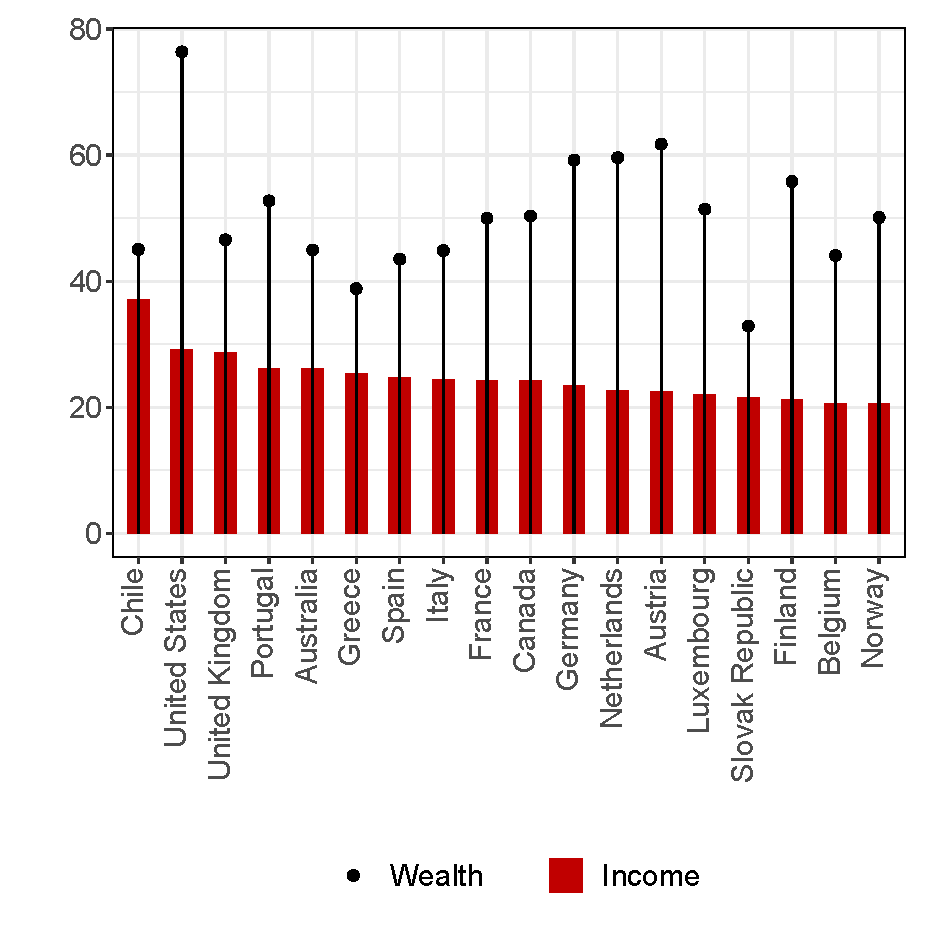
\includegraphics[width=0.9\textwidth]{figures/ch3/wealthincome_comp_oecd.eps}
        \label{ch3fig:wealthincome_comp_oecd}
        \begin{minipage}{0.8\textwidth}
          \footnotesize
          \emph{Source: Author based on the \ac{OECD}}
          \end{minipage}
    \end{figure}
    
    \newpage
    \section{Bayesian Model Averaging}
    \label{ch3sec:app_bma}
    First, consider the following linear model:
    %
    % OLS notation
    \begin{equation}\label{ch3eq:OLS}
    y = \alpha + X\beta+ \varepsilon \qquad \varepsilon  \sim\ N(0, \sigma^{2}I)
    \end{equation}
    %
    where $y$ represents a dependent variable, $\alpha$ is a constant, $X$ is the matrix of explanatory variables, $\beta$ represents the corresponding coefficients, and $\varepsilon$ is a vector of normally distributed \ac{IID} error terms with variance $\sigma^{2}$. 
    
    \ac{BMA} takes into consideration all possible combinations of $X$ from equation \ref{ch3eq:OLS} and takes a weighted average of the estimated coefficients. Even with a modest-sized regression model, the number of combinations rises dramatically, and even with current computers, it is impossible to estimate all regression models. For this reason, a subset of models is considered, and an \ac{MCMC} sampler is employed (we discuss the sampler in detail below). The substructure of the model is as follows:
    %
    % submodel structure
    \begin{equation}\label{ch3eq:OLSsub}
    y = \alpha_{i} + X_{i}\beta_{i}+ \varepsilon \qquad \varepsilon  \sim\ N(0, \sigma^{2}I)
    \end{equation}
    %
    $X_{i}$ corresponds to a subset of $X$, and $\alpha_{i} $ and $ \beta_{i}$ are the corresponding coefficients. If the number of regressors is $K$, the total number of models equals $2^{K}$, and $i \in [1,2^{K}]$. 
    
    Bayes' rule implies that
    %
    % Bayes' rule with 'model' notation
    \begin{equation}\label{ch3eq:BRmodel}
    p(\beta \vert y,X) = \frac{p(y,X\vert \beta)p(\beta)}{p(y,X)}
    \end{equation}
    where $p(\beta \vert y, X)$ is the posterior density, $p(y, X\vert \beta)$ is the marginal likelihood (ML), $p(\beta)$ is the prior density, and $p(y,X)$ is the probability of the data. 
    
    The individual regression models are denoted as $M_{1},...,M_{i}$. In the case of $K$ regressors, there are $M_{1},...,M_{i}$ regression models, where $i \in [1,2^{K}]$. The model is formed using a likelihood function and a prior density, where $M_{i}$ depends on the parameters $\beta_{i}$, with a posterior probability to be derived in the following manner:
    \begin{equation}\label{ch3eq:BROM}
    p(\beta_{i} \vert M_{i},y,X) = \frac{p(y\vert \beta_{i},M_{i},X)p(\beta_{i}\vert M_{i})}{p(y \vert M_{i},X)}
    \end{equation}
    Next, we describe the averaging principle of \ac{BMA} and individual components of equation \ref{ch3eq:BRmodel}.
    %
    %%
    \subsection*{Posterior Model Probability}
    %%
    %
    The \ac{PMP} provides the weights for averaging model parameters across the individual models. The \ac{PMP} also arises from Bayes' theorem:
    
    \begin{equation}\label{ch3eq:PMPmain}
    p(M_{i} \vert y,X) = \frac{p(y\vert M_{i},X)p(M_{i})}{p(y \vert X)}
    \end{equation}
    
    where $p(y\vert M_{i},X)$ is the \ac{ML} of the model (i.e., the probability of the data given the model $M_{i}$), $p(M_{i})$ is the prior model probability, and $p(y\vert X)$ is the integrated likelihood. The term in the denominator is typically disregarded because it is constant across all models under consideration. The \ac{PMP} then becomes directly proportional to ML and the prior probability. The prior probability $p(M_{i} \propto 1)$ is typically set to acknowledge that the `true' model is unknown.
    % Proportionality of PMP
    \begin{equation}
    p(M_{i}\vert y,X) \propto p(y\vert M_{i},X)p(M_{i})
    \end{equation}
    %
    We discuss the calculation of ML in detail in section \ref{ch3sec:ML}. Researchers must set the model prior to reflect the beliefs regarding the data before inspecting them. 
    %
    \subsection*{Posterior Mean}
    The parameter point estimates are derived within the Bayesian framework as follows. \textcite{Zeugner2011} and \textcite{MoralBenito2012} show that the weighted posterior distribution of any statistic (most notably the $\beta$ coefficients) is obtained as follows:
    %
    %% Posterior distribution of the coefficients
    \begin{equation}\label{ch3eq:parest}
    p(\beta \vert y, X) = \sum_{i=1}^{2^{K}} p(\beta_{i} \vert M_{i},y,X)p(M_{i} \vert y,X)
    \end{equation}
    
    where $p(M_{i} \vert y, X)$ is the \ac{PMP} of the corresponding model $M_{i}$ from equation \ref{ch3eq:PMPmain}. The point estimates are obtained by taking expectations:
    
    \begin{equation}\label{ch3eq:pointparest}
    E(\beta \vert y, X) = \sum_{i=1}^{2^{K}} E(\beta_{i} \vert M_{i},y,X)p(M_{i} \vert y,X)
    \end{equation}
    
    $E(\beta \vert y, X)$ represents the average coefficient, and $E(\beta \vert M_{i},y,X)$ is the estimate of the $\beta_{i}$ coefficients from model $M_{i}$. The posterior distribution of the coefficients depends on the choice of the prior $g$. \textcite{Zeugner2011} expresses the expected value of the parameter in $M_{i}$ as follows:
    \begin{equation}\label{ch3eq:postdist}
    E(\beta_{i} \vert y,X,g,M_{i}) = \frac{g}{1+g}\hat{\beta_{i}}
    \end{equation}
    with $\hat{\beta_{i}}$ corresponding to the standard OLS estimate.
    
    \subsection*{Posterior Variance}
    \textcite{MoralBenito2012} provides a formula for the variance corresponding to the expected values of the coefficients derived in the previous subsection:
    \begin{equation}\label{ch3eq:postvar}
    \begin{aligned}
    Var(\beta \vert y, X) &= \sum_{i=1}^{2^{K}} p(M_{i} \vert y,X)Var(\beta_{i} \vert M_{i},y,X) \\ 
    & +\sum_{i=1}^{2^{K}}p(M_{i} \vert y,X){(E(\beta_{i}\vert M_{i},y,X)-E(\beta \vert y, X))}^{2}
    \end{aligned}
    \end{equation}
    The variance consists of two terms: the weighted average of variance estimates across different models $Var(\beta_{i} \vert M_{i},y,X)$ and the weighted variance across different models in the second component ${{E(\beta_{i}\vert  M_{i},y,X)}-{E(\beta \vert y,X))}}^{2}$. $E(\beta \vert y,X)$ represents the posterior mean from equation \ref{ch3eq:pointparest}. As a result, \ac{BMA} accounts for uncertainty regarding the parameter estimates that arise due to differences across models in addition to the uncertainty of individual models. \textcite{Zeugner2011} derives how the value of the prior $g$ affects the posterior variance of the parameters:
    %
    % Posterior variance of betas
    \begin{equation}\label{ch3eq:postvarZ}
    Cov(\beta_{i}\vert y,X,g,M_{i}) = \frac{(y-\bar{y})'(y-\bar{y})}{N-3} \frac{g}{1+g} \left( 1- \frac{g}{1+g}R_{i}^{2} \right) (X_{i}'X_{i})^{-1}
    \end{equation}
    where $\bar{y}$ denotes the mean of vector $y$, $N$ is the sample size, and $R^{2}_{i}$ is the R-squared value corresponding to the model $i$.
    %
    %%
    \subsection*{Marginal Likelihood}\label{ch3sec:ML}
    ML can be calculated using equation \ref{ch3eq:BROM} for each model $M_{i}$. Both sides of the equation must be integrated with respect to $\beta_{i}$. Employing $\int_{\beta} p(\beta_{i}\vert M_{i},y,X) \, d\beta_{i}=1$, it follows that
    %
    % Marginal likelihood basic
    \begin{equation}\label{ch3eq:ML}
    p(y \vert  M_{i},X) = \int_{\beta}{p(y \vert \beta_{i},M_{i},X)p(\beta_{i} \vert M_{i},X) \, d\beta_{i}}
    \end{equation}
    %%
    The above equation illustrates the general textbook derivation, but the computation depends on the elicited priors. \textcite{Zeugner2011} employs the ``Zellner's g prior'' structure, which we also utilize in this paper. The ML for a single model can then be expressed using the prior as in \textcite{FeldkircherZeugner2009}:
    \begin{equation}\label{ch3eq:MLFZ}
    p(y \vert  M_{i},X,g) = \int_{0}^{\infty}{\int_{\beta}{p(y \vert \beta_{i}, \sigma^{2},M_{i})p(\beta_{i},\sigma^{2} \vert g) \, d\beta d\sigma}}
    \end{equation}
    Furthermore, \textcite{FeldkircherZeugner2009} show that ML is in this case simply proportional to
    %
    % Marginal likelihood using g prior, from Zeugner 2011
    \begin{equation}
    \label{ch3eq:MLg}
    p(y \vert M_{i}, X, g) \propto (y-\bar{y})'(y-\bar{y})^{- \frac{N-1}{2}} (1+g)^{- \frac{k_{i}}{2}} \left(1- \frac{g}{1+g}R^{2}_{i} \right)^{- \frac{N-1}{2}}
    \end{equation}
    In this equation, $R^{2}_{i}$ is the R-squared of model $M_{i}$, and $k_{i}$ is the number of explanatory variables in model $i$ introduced to include a size penalty for the model. $N$ and $\bar{y}$ are the same as in equation \ref{ch3eq:postvarZ}, i.e., the number of observations and the mean of vector $y$, respectively.
    %%
    %%
    \subsection*{Posterior Inclusion Probability}
    The standard \ac{BMA} framework provides the \ac{PIP}, which indicates the probability that a particular regressor is included in the ``true'' model. The \ac{PIP} is the sum of the \acp{PMP} of the models including the variable $k$:
    \begin{equation}\label{ch3eq:PIP}
    PIP = p(\beta_{k} \neq 0 \vert y, X) = \sum_{i=1}^{2^{K}} p(M_{i} \vert \beta_{k} \neq 0, y, X)
    \end{equation}
    
    \subsection*{\ac{MCMC} Sampler}
    \label{ch3sec:mc3}
    One of the limitations of \ac{BMA} is its computational difficulty when the number of potential regressors $K$ becomes very large. Historically, the computational burden has been the primary factor preventing researchers from employing Bayesian methods. \textcite{Zeugner2011} notes that for small models, it is possible to enumerate all variable combinations. However, when $K > 25$, it becomes impossible to evaluate the entire model space within a reasonable time frame. In such cases, \ac{BMA} utilizes MC$^{3}$ samplers to approximate the crucial part of the posterior model distribution containing the most likely models. \ac{BMA} applies the Metropolis-Hastings algorithm, which is outlined in \textcite{Zeugner2011} as follows:
    
    At any step $i$, the sampler is currently at model $M_{i}$, having \ac{PMP} $p(M_{i} \vert y,X)$. In the next step $i+1$, model $M_{j}$ is proposed to replace $M_{i}$. The sampler accepts the new model $M_{j}$ with the following probability:
    \begin{equation}\label{ch3eq:sampler}
    p_{i,j} = min \left( 1, \frac{p(M_{j} \vert y,X)}{p(M_{i} \vert y,X)}\right)
    \end{equation}
    If model $M_{j}$ is rejected, the next model $M_{k}$ is suggested and compared with $M_{i}$. With an increasing number of iterations, the number of times each model is retained converges to the distribution of posterior model probabilities. Typically, one of the following MC$^{3}$ samplers is used to construct the models:
    %
    \begin{itemize}
        \item{Birth-death sampler - randomly chooses one of the explanatory variables, which is included if it is not already part of the current model $M_{i}$ or dropped if it is already in $M_{i}$.}
        %
        \item{Reversible-jump sampler - with 50\% probability, the birth-death sampler is used to determine the next candidate model. With 50\% probability, the sampler randomly swaps one of the covariates in $M_{i}$ for a covariate previously excluded from $M_{i}$.}
    \end{itemize}
    %
    Because the sampler can begin with a ``poor'' model with low \ac{PMP}, the predefined number of initial draws, the so-called burn-ins, are usually dropped. The quality of the approximation can be evaluated on the basis of the correlation between the \ac{PMP} derived from an analytical approach and those obtained from the MC$^{3}$ sampler. It depends on the number of iterations (draws) and the likelihood of the initially selected model. \textcite{Zeugner2011} notes that a \ac{PMP} correlation of approximately 0.9 indicates a ``good degree of convergence''. In the event that the correlation is lower, the number of sampler iterations should be increased.
  \end{subappendices}
\end{refsection}
\begin{refsection}
\chapter{Finance and Inequality - panel BMA approach}
\label{ch4}
\blfootnote{The author acknowledges support from Charles University Research Centre program No. UNCE/HUM/035}

\begin{quote}
\begin{center}\textbf{Abstract}\end{center}
	We investigate the impact of financial development on income inequality differentiating between depth, efficiency and access to financial markets and institutions. We apply panel Bayesian model averaging framework to address model uncertainty to reveal that financial development has complex influence on the income distribution within countries. The access to and efficiency of banking decrease income inequality. The size of the markets has no influence on overall income inequality, but contributes to the increasing top income shares. Moreover, unemployment along with investment into non-tangible assets increase income inequality while higher redistribution and physical capital investment imply lower levels of inequality.  
	\end{quote}

\newpage
\section{Introduction}
\label{ch4sec:intro}
% Financial development alters how much are economic opportunities depend on the individual skills, family endowments, social status or political connections. Individual depend on financial system to provide loans to start new business, attain education

Finance captures the capacity of financial intermediaries and markets to screen investment opportunities, monitor the debtors who were provided funding, as well as pooling and management of risk. With inequality, we focus in the paper on the inequality in the distribution of income. Arguably, the literature discusses other concepts of inequality, e.g. intergenerational persistence of relative income differences or equality of opportunity \parencite{demirgucc2009finance}.

\textcite{claessens2007finance} argue that although deeper financial systems generally provide better opportunities of access to finance, the relationship is not universal.

The average income inequality rose across \ac{OECD} by 1.4 percentage points \parencite{oecd2013crisis}.

\section{Related literature}
\label{ch4sec:literature}
The research in the area of financial development and income inequality is well established. \textcite{demirgucc2009finance}, \textcite{claessens2007finance}, and more recently \cite{de2017finance} provide extensive reviews of the topic. A similar theme emerges in all three papers. The implications from theoretical contributions provide conflicting predictions about the relationship and empirical results bring evidence for both positive and negative effect. Although majority of the papers point towards finance tightening the distribution of income this results is not universal with some papers suggesting the opposite while other stress potential non-linearities.

A key divide appears between the effect of financial development on extensive and intensive margin. The extensive margin captures the extend to which individuals, who had not been using financial services before, gain access. On the other hand, the intensive margin describes growing use of finance by the agents who had already been using it before \parencite{demirgucc2009finance}. Financial development on the extensive margin might lead to more equal opportunities and outcomes. Access to credit by previously disadvantaged groups allows human capital accumulation \parencite{galorzeira1993income, galormoav2004, braunetal2019}, formation and growth of new firms \parencite{evans1989estimated,banerjeenewman1990}, with more evenly distributed economic opportunities as a result\footnote{Having similar economic opportunities might decrease the cross-generational inequality, by diminishing the effect of e.g. parental wealth. Depending on the innate abilities and talents of the individuals, however, it may increase the inequality of income within every generation at the same time.}.

On the contrary, intensive margin of financial development might disproportionately benefit the rich who may leverage financial services for their further benefit or to protect their existing rents. \textcite{GreenwoodJovanovic1990} present a model where the finance is the key driver of inequality and the welfare gains accrued by the incumbents - primarily the rich - in the initial development stage. With time, more agents meet the fixed costs of joining the financial intermediaries and they enjoy higher returns. Consequently, the efficiency of resource allocation also increases, which enhances growth and reduces inequality. \textcite{perotti2007investor} present a framework based on political economy. They argument depends on a lobby for lower investor protection to prevent entrance of the new competitors. The politicians require higher bribe from the lobbyist the greater is their accountability for policy decisions. Thus, with increasing accountability, investor protection strengthens and spurs market entry and competition. The authors examine their prediction in a cross-section and show that better investor protection correlates with larger entry rates and higher firm density in more financially intensive sectors\footnote{In addition, they show that the most important factor of accountability is not the formal measure of democratic institutions, but newspaper readership which they interpret as broad awareness of policy choices and their outcomes.}. 

Financial development may also have indirect effect on income inequality through economic growth. \textcite{townsendeueda2006} model how finance interacts with production and allocation of credit. If increased use of finance increases the demand for low- relatively to the high-skilled workers, then it may have equalizing consequences for income distribution. Empirical evidence by \textcite{beck2010big} show that bank deregulation and increased competition in loan provision in the \ac{US} primarily benefited the workers with income below the median. Similarly, \textcite{delis2014} provide evidence of bank deregulation and liberalization tightening the income distribution, although this effect is only present in countries with high-quality institutions. They attribute the effect to the changes in labour market conditions and relatively higher wages and working hours of the low-skilled workers following the reforms. 

A set of distinct papers explores the relationship between inequality and growth while stressing financial markets imperfections driving the outcomes. Income inequality and growth may intersect through varying channels. Accumulation of savings, unobservable effort, and investment project size favor the prediction of growth inducing inequality. Negative impact of inequality on human capital accumulation, entrepreneurial activity provide argument for the opposing view. 
\textcite{van2018inequality} report how income inequality in the \ac{US} has different implications for the future income growth of the rich and the poor. High inequality seems to hurt the prospects of the poor while the top of the distribution is unaffected. The rich thus disproportionately benefit from higher inequality as their subsequent income exhibit faster growth. The authors attribute this effect to the political channel the rich use to lobby in favor of the policies which support their economic interests. Preferences of the rich are ultimately more likely to determine public policy than the preferences of the majority \parencite{gilens_page_2014}. High inequality together with a credit constraint and rich driving the political process results in low government spending and lasting inequality.

The literature does not converge on the conclusions even in the empirical cross-country and panel data studies. The papers link higher levels of financial development with lower levels of inequality \parencite{beck2007finance, hamori2012, gimet2011closer, kunieda2014finance}\footnote{For an extended list, we refer to \textcite{de2017finance}.}. On the other hand, several other estimate a inequality inducing effect of finance \parencite{Jaumotte2013, jauch2016financial, de2017finance}. Finally, some authors claim there the relationship might be non-linear, conditional on a threshold value of financial development \parencite{kim2011nonlinearity,tan2012nonlinear} or institutional quality \parencite{LawSingh2014, delis2014}.

Three papers are the closest to ours, each in a different respect. First, \textcite{de2017finance} examine different dimensions of finance on income inequality. Their results suggest that financial development, financial liberalization, and banking crises all increase pre-tax income inequality within countries. Additionally, they show that the effect of financial liberalization is conditional on democratic accountability. Higher accountability mitigates the impact of liberalization on inequality. On the contrary, the financial development, proxied by the credit to GDP ratio, has inequality increasing effect irrespective of the institutional background. Second, \textcite{naceurzhang2016} take similar approach in considering multiple dimensions --- the access, efficiency, and stability of the financial sector, although not examining the indicators simultaneously.  Third, \textcite{furceri2019robust} apply \ac{WALS} to identify robust determinants of income inequality. Their approach mirrors ours in accounting for model uncertainty in the estimation. Their focus is more general rather than focused primarily on finance. We provide synthesis and extension to these papers in providing more detailed view on the link between finance in shaping income inequality and examining multiple measures of inequality while specifically identifying the determinants of top income shares along with the determinants of the overall income distribution\footnote{Captured by income Gini index.}.

% An exemption from focus solely on the size of financial sector is the study by \textcite{naceurzhang2016} which applies a similar approach to ours, taking into consideration the access, efficiency, and stability of the financial sector. However, there are severe limitation to their study. First, their coverage does not correspond to the availability of the data. Second, they do not account for the different dimensions of finance simultaneously and always use a single indicator of development at a time. Third, they do not explicitly differentiate between the banking sector and financial markets. We provide a more detailed as well as more robust picture of the financial development effect on finance in these dimensions.

% \textcite{de2017finance} examine different dimensions of finance on income inequality. Their results suggest that financial development, financial liberalization, and banking crises all increase market income inequality within countries. Additionally, they show that the effect of financial liberalization is conditional on democratic accountability. The higher the accountability, the less severe is the negative impact of liberalization on inequality. On the contrary, the financial development, proxied by the credit to GDP ratio, has inequality increasing effect irrespective of the institutional background.

% \textcite{furceri2019robust} apply WALS to identify robust determinants of income inequality. They are the closest paper to ours since they account for model uncertainty in the estimation. Their focus if more general rather than on finance specifically. Out work offers more detailed contribution in terms of the role of finance in shaping income inequality. On the top of that, we differ from their analysis by examining multiple measures of inequality and specifically identifying the determinants of top income shares along with the determinants of the overall income distribution represented by income Gini index. We provide further evidence in all these dimensions.

%
%
%
%
%

\section{Data}
The key variable in the paper is the measure of income inequality. We want to examine how financial development affects income inequality and whether the effect might by different at the top quantiles of income distribution. As the overall measure of income inequality, we rely the after-tax Gini coefficient from \ac{SWIID} by \textcite{Solt2019}, which is a standard resource in the literature\footnote{There are alternative sources of for Gini coefficient, e.g. \ac{WIID} or \ac{LIS}, but each of them brings limitations in terms of comparability or coverage.}. Its critical advantage lies in the widespread coverage across countries and time and a unified methodology which provides a reasonable level of comparability. It typically takes values in the interval between 0 and 100 where the former suggests perfect equality (everyone in the economy enjoys the same income) and the latter perfect inequality (all the income goes to only a single unit). We depart from existing papers slightly in considering the after-tax rather than the before-tax income distribution as a dependent variable. 

To explore the relationship in the top part of the distribution, we choose top income share from \ac{WID}\footnote{The methodology and guidelines to database are provided by \textcite{alvaredo2016distributional}.}. The surveys suffer from well-known issues of underrepresentation of the top income earners and the distortions resulting from self-reported character of the data. This can influence not only the top income shares resulting from survey data, but also distortions in the overall measures of inequality. The data in \ac{WID} make use of income tax records in individual countries and the derived shares obtained using consistent methodology of \ac{DINA} are arguably more reliable relative to the survey-based measures which are the primary source of majority estimates of income distributions. 

The data spans from 2000 to 2014. We follow the literature \parencite{dabla2015causes,de2017finance} and average both the inequality measure (dependent variable) and the potential determinants (independent variables) across three year intervals. There are important reasons for looking at the averages than observation in individual years. Annual macroeconomic data are subject to fluctuations and the data on income inequality is noisy \textcite{delis2014}. Averaging should diminish the level of noise. On the top of that, the variables at the center of our analysis, e.g. stock market capitalization or credit to \ac{GDP}, are likely to be affected by the business cycles and volatile on the yearly basis. Similar argument holds for top income shares, as they depend, among other things, on the bonuses paid out each year and capital income. We want to explore the long-term rather than the short-term relationship and that guides the choice of averaged data. Faced against the trade-off between length of the averaging periods and available observations in the time dimension, we take a compromise of three years in contrast to the literature, where generally the 5-year intervals apply. The availability of financial development indicators limits the analysis to a period from 2000 onward and we prefer to keep at least 5 unique time periods to just three under the case of 5-year average\footnote{Nevertheless, we run the estimation with 5-year averages of data as a robustness check and find no critical qualitative differences compared to the baseline.}.

Table \ref{ch4tab:sum} report the summary statistics of the income inequality variables and financial development indicators.

% \begin{table}[ht!]
%     \small
%     \caption{Summary statistics of inequality variables}
%     \label{ch4tab:ineq}
%     \centering
%        \begin{tabular}{lrrrr}
%         \toprule
%         Variable & Mean & St. Dev. & Min & Max \\
%         \midrule
%         After-tax Gini index  & & & & \\
%         Top 10\% income share & & & & \\
%         Top 1\% income share & & & & \\
%         \bottomrule
%     \end{tabular}
% \end{table}

\begin{table}[ht!]
  \small
  \caption{Summary statistics of selected variables}
  \label{ch4tab:sum}
  \centering
     \begin{tabular}{lrrrr}
      \toprule
      Variable & Mean & St. Dev. & Min & Max \\
      \midrule
      After-tax Gini index  & 36.38 & 8.12 & 22.88 & 61.16 \\
      Top 10\% income share & 0.42 & 0.12 & 0.24 & 0.71 \\
      Top 1\% income share & 0.14 & 0.06 & 0.05 & 0.38 \\
      FIA & 0.42 & 0.32 & 0.01 & 1.00 \\
      FIE & 0.60 & 0.13 & 0.11 & 0.81 \\
      FID & 0.37 & 0.30 & 0.01 & 1.00 \\      
      FMD & 0.33 & 0.32 & 0.00 & 0.99 \\
      \bottomrule
  \end{tabular}
\end{table}
%
%
%
%
%

\begin{table}[htbp!]
  \small
  \caption{Correlation matrix of selected variables}
  \label{ch4tab:corr}
  \centering
  \begin{tabular}{lrrrrrrr}
    \toprule
  %  & GiniNet & Top10share & Top1share & FIA & FIE & FID & FMD \\
    % \midrule
    After-tax Gini index  & . &  &  &  &  &  &  \\
    Top 10\% income share & 0.47 & . &  &  &  &  &  \\ 
    Top 1\% income share & 0.39 & 0.84 & . &  &  &  &  \\
    FIA & -0.14 & -0.09 & -0.12 & . &  &  &  \\
    FIE & -0.14 & -0.10 & -0.06 & 0.28 & . &  &  \\ 
    FID & -0.07 & 0.12 & 0.06 & 0.60 & 0.24 & . &  \\
    FMD & 0.03 & 0.2 & 0.13 & 0.36 & 0.1 & 0.40 & . \\ 
     \bottomrule
  \end{tabular}
  \end{table}

We obtain the financial development indicators from \ac{GFDD}. The database offers detailed indicators along four dimensions of financial systems and allows to estimate the affect of changes in access, size, efficiency, and stability of financial markets. Furthermore, we can distinguish between banking sector and financial markets in all these dimensions. The data in for access and stability of stock markets remains sparse in the concerned period we must leave them out of analysis. We use the version of financial indicators from \cite{svirydzenka2016introducing}. The authors make use of principal component analysis in order to construct aggregate indicators in each characteristic of financial sector. In summary, we have indicators of financial institutions depth (FID), financial markets depth (FMD), access to financial institutions (FIA), efficiency of financial markets (FME), and institutions (FIE)\footnote{\textcite{svirydzenka2016introducing} extrapolate the indicators from top to bottom if the original variables are unavailable, we make sure that that at least one variable is available for the construction of the index and no artificial correlation introduced to the data.}. We report the composition of each indicator in Table \ref{ch4tab:finind}. 

\begin{figure}
  \caption{Gini Coefficient and top shares}
  \label{ch4fig:gini_topshares}
  \centering
  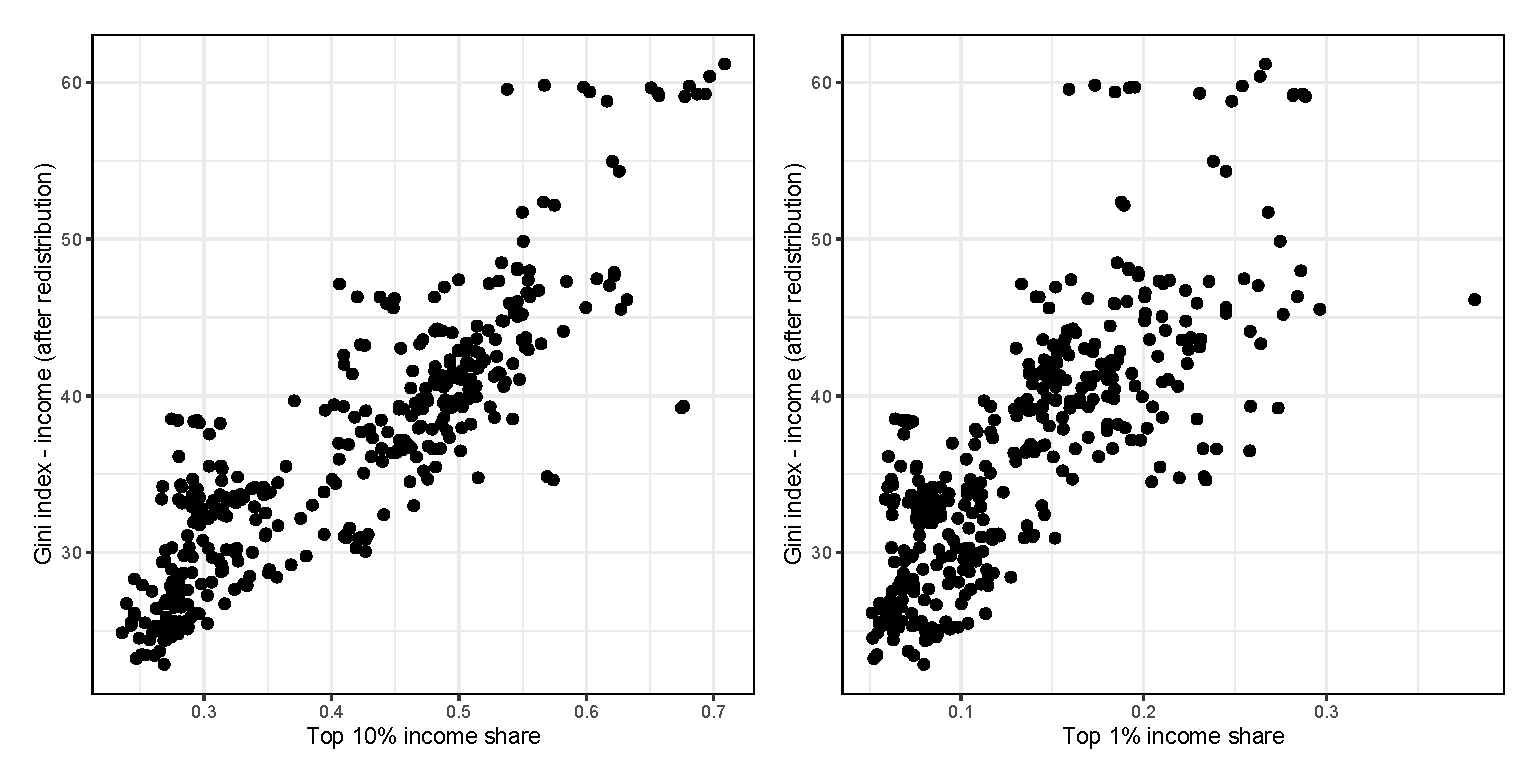
\includegraphics[width=0.8\textwidth, keepaspectratio]{figures/ch4/plots_ineq}
\end{figure}

% Figure \ref{ch4fig:gini_findev} shows the scatter plots of all the available observations after averaging between Gini coefficient and selected financial indicators. Although the data is noisy, it suggest negative correlation between the variables. Figure \ref{ch4fig:gini_findev_dm} then shows the corresponding scatter plots of the data which was demeaned using the within country averages over time. %The relationship between Gini and financial indicators appears considerably weaker following the transformation, with the exception of access to financial institutions where visual inspection allows pointing to a negative correlation.

We build the choice of other explanatory variables on a reviews of income inequality drivers \parencite{roineetal2009,nolan2019drivers}, related study of finance-inequality nexus \parencite{de2017finance}, and a more general inquiry into the robust determinants of income inequality \parencite{furceri2019robust}. The potential regressors could be categorized in several groups. They control for economic and financial development, demographics, globalization, and institutional background. Table \ref{ch4app:exog} reports all the control variables and their sources. 

% \textcite{nolan2019drivers} bring a survey of the literature on determinants of inequality, summarizing the complexity of the inequality dynamics. They stress that many of the determinants are interlinked which implies difficulty in assigning precise effects to individual drivers of inequality. Additionally, they encourage complementary individual country case studies to support the finding of the general cross-country estimates.

% Both theoretical and empirical studies leave out the issue of importing the financial services from abroad. We include financial globalization from KOF among our control variables.
%
%
\section{Methodology}
\label{ch4sec:methodology}

\section{Results}
\label{ch4sec:results}
We examine the determinants of inequality in the panel \ac{BMA} framework and present the results in the following sections. We start with a model where we capture the overall inequality by Gini index in subsection \ref{ch4subsec:gini}. We then continue to estimations where we consider the shares of income going to the top 10\% and top 1\% of the income distribution as our dependent variable. We check the robustness of our estimates by employing alternative model and parameter priors throughout the analysis.

\subsection{Gini index of inequality}\label{ch4subsec:gini}
We focus the analysis on the relationship between the indicators representing various aspects of financial development and income inequality. Figure \ref{ch4fig:gini_findev_dm} outlines the expected link after we have demeaned the variables using the cross-sectional averages. The relationship is not particularly strong, but we observe negative correlation between Gini index and indicators of access and efficiency of financial institutions, as suggested by a linear estimate. For size indicators of financial market and institutions, the link appears much weaker.

\begin{figure}[htbp!]
  \caption{Gini Coefficient and Financial Development Indicators}
  \label{ch4fig:gini_findev_dm}
  \centering
  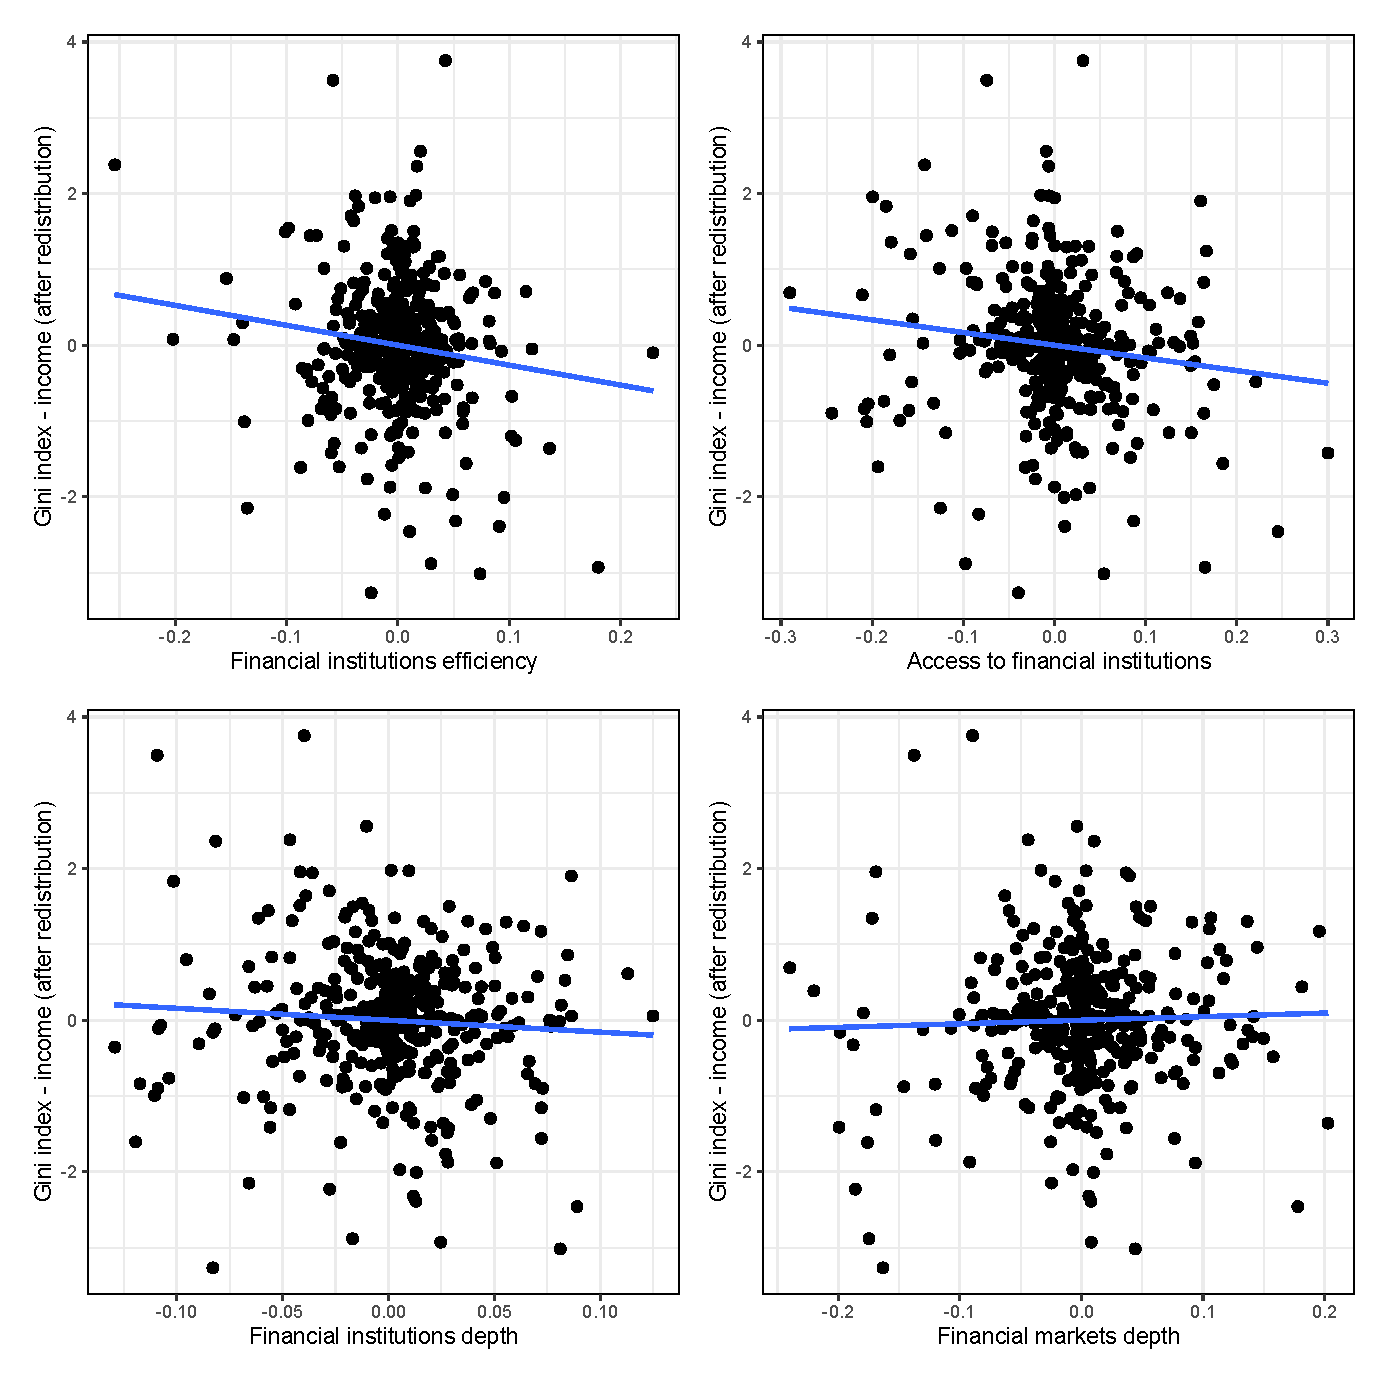
\includegraphics[width=0.8\textwidth, keepaspectratio]{figures/ch4/plots_findev_gini_dm}
\end{figure}

Table \ref{ch4res:baseline_gini} reports the baseline results. The baseline estimate relies on the uniform model prior and hyper-g parameter prior. We choose the model prior to remain agnostic about the prior probability of each examined model. While uniform prior assigns the same prior probability to each model, the distribution of the prior model space is concentrated around $k/2$, where $k$ is the number of potential covariates and consequentially the estimate may gravitate towards larger model sizes and higher number of covariates\footnote{See \textcite{LeySteel2009} for details.}. The hyper-g prior provides more robust results than some other traditionally applied $g$ priors \parencite{feldkircher2012impact}. Overall, we have 16 variables with \ac{PIP} above 0.8. The number of unique relevant regressors effectively shrinks by two if we abstract from the quadratic terms of the \ac{GDP} per capita and the education index. Most of the estimated posterior means exhibit expected signs.

The only financial indicators which occur among the top regressors are access and efficiency of financial institutions with \acp{PIP} of 1 and 0.88, respectively. The posterior mean on the coefficients in both dimension is negative so higher levels of access and efficiency are associated with lower levels of income inequality. The inequality decreasing effect of access to finance on inequality mirrors \textcite{hasan2020finance} for wealth inequality, and partially also \textcite{furceri2019robust} who document similar effect, although not fully robust. The observation on inequality decreasing effect of access to finance supports also \textcite{claessens2007finance} who suggest that access may equalize economic opportunities and lead to more evenly distributed income. The efficiency of financial intermediation putting downward pressure on income inequality also has a precedent in \textcite{gimet2011closer}\footnote{They measure efficiency of banking sector by the difference between lending rate and the deposit rate (spread). They argue higher spread reflects low competition and high transaction costs. The imperfections in the credit market can skew the credit to high-income, wealthy households who can provide significant collateral, reinforcing the existing inequality.}. We fail to confirm that the efficiency of financial institutions is a robust determinant of inequality, however, as the \ac{PIP} markedly decreases under alternative model priors. None of the size indicators of financial institutions or markets has high probability of inclusion. 

Education expenditures (\%share of \ac{GDP}) along with the education index calculated using mean and expected years of schooling show inequality decreasing effect. This is in line with prediction of \textcite{goldin2009race,deaton2013great} who claim that the skill-biased technological change should be mitigated by education. \textcite{furceri2019robust} provide similar evidence using the levels of education attainment. 

% \begin{figure}
%   \caption{Gini Coefficient and Financial Development Indicators}
%   \label{ch4fig:gini_findev}
%   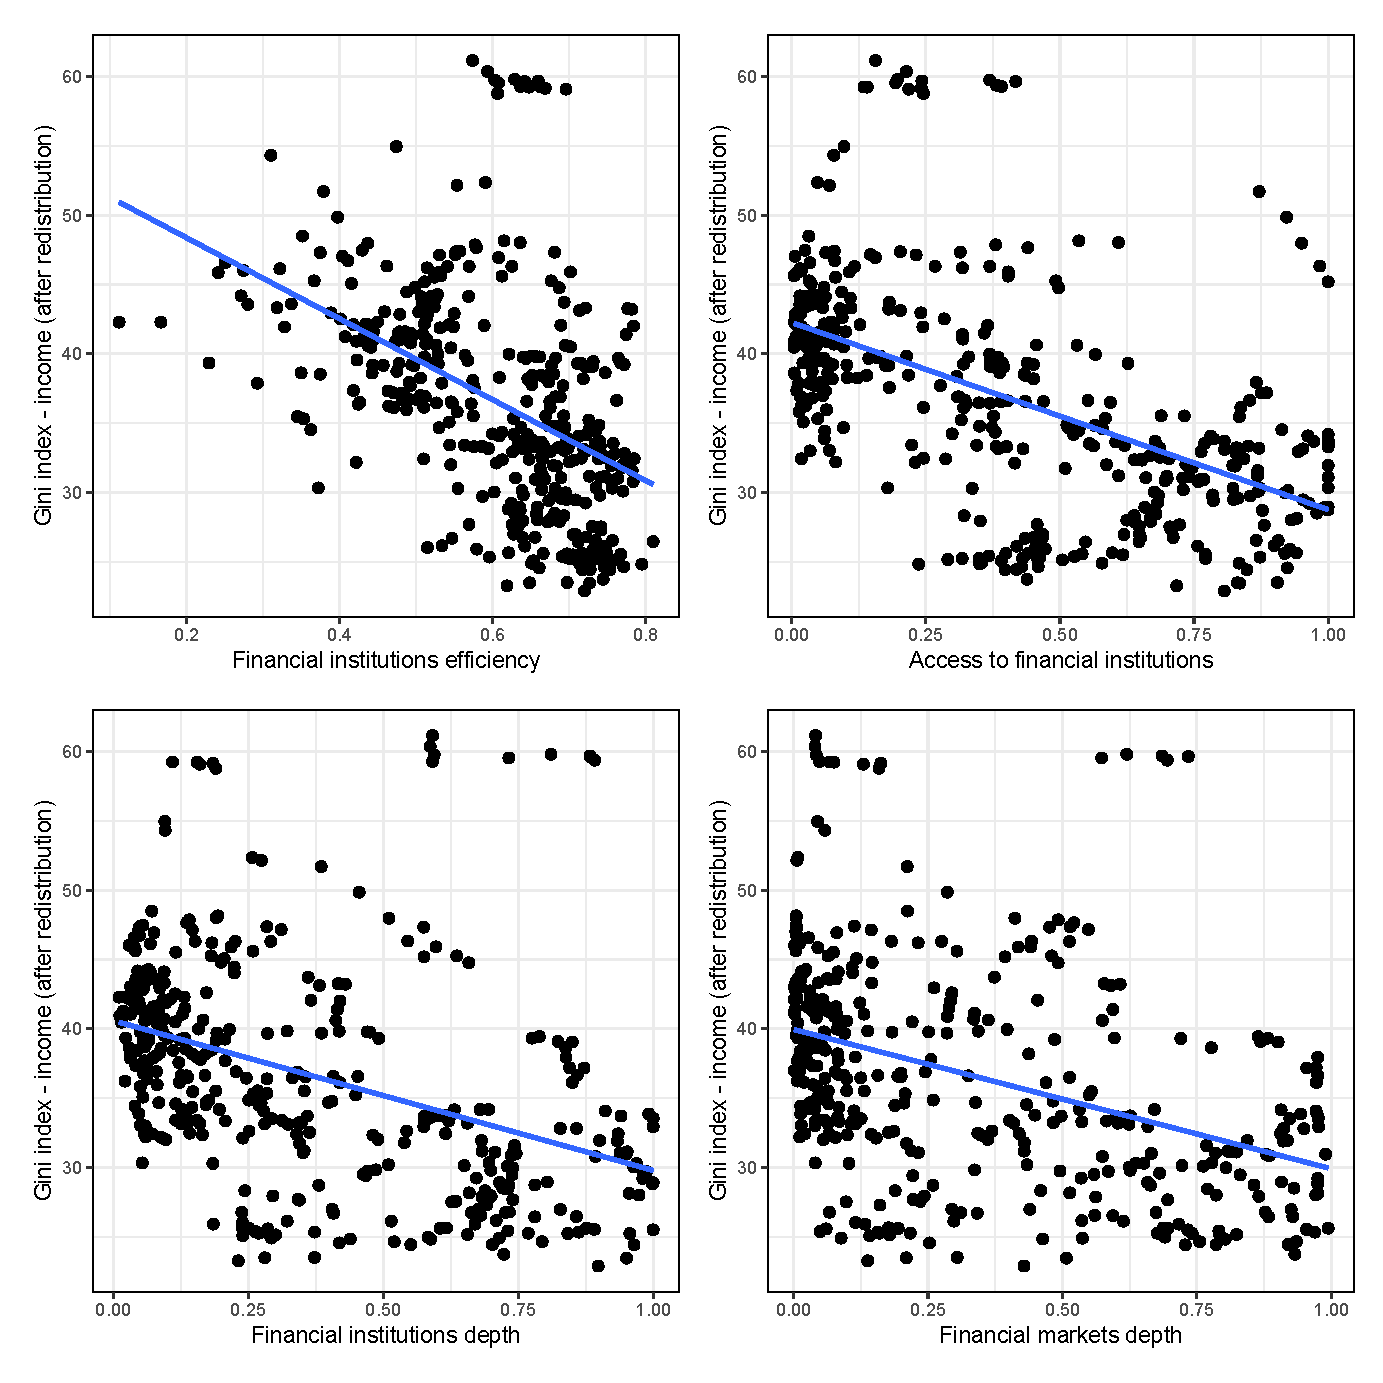
\includegraphics[width=\textwidth, keepaspectratio]{figures/ch4/plots_findev_gini}
% \end{figure}

The benefits of capital markets liberalization seem to be concentrated to the top of the income distribution. Top quintile of the distribution accrues nearly all of the income growth following the liberalization while the share of middle three quantiles decreases and the bottom remains unaffected \parencite{das2003income}.

\begin{figure}[htbp!]
  \caption{Robustness checks with alternative model priors, Gini coefficient}
  \label{ch4fig:gini_comp}
  \centering
  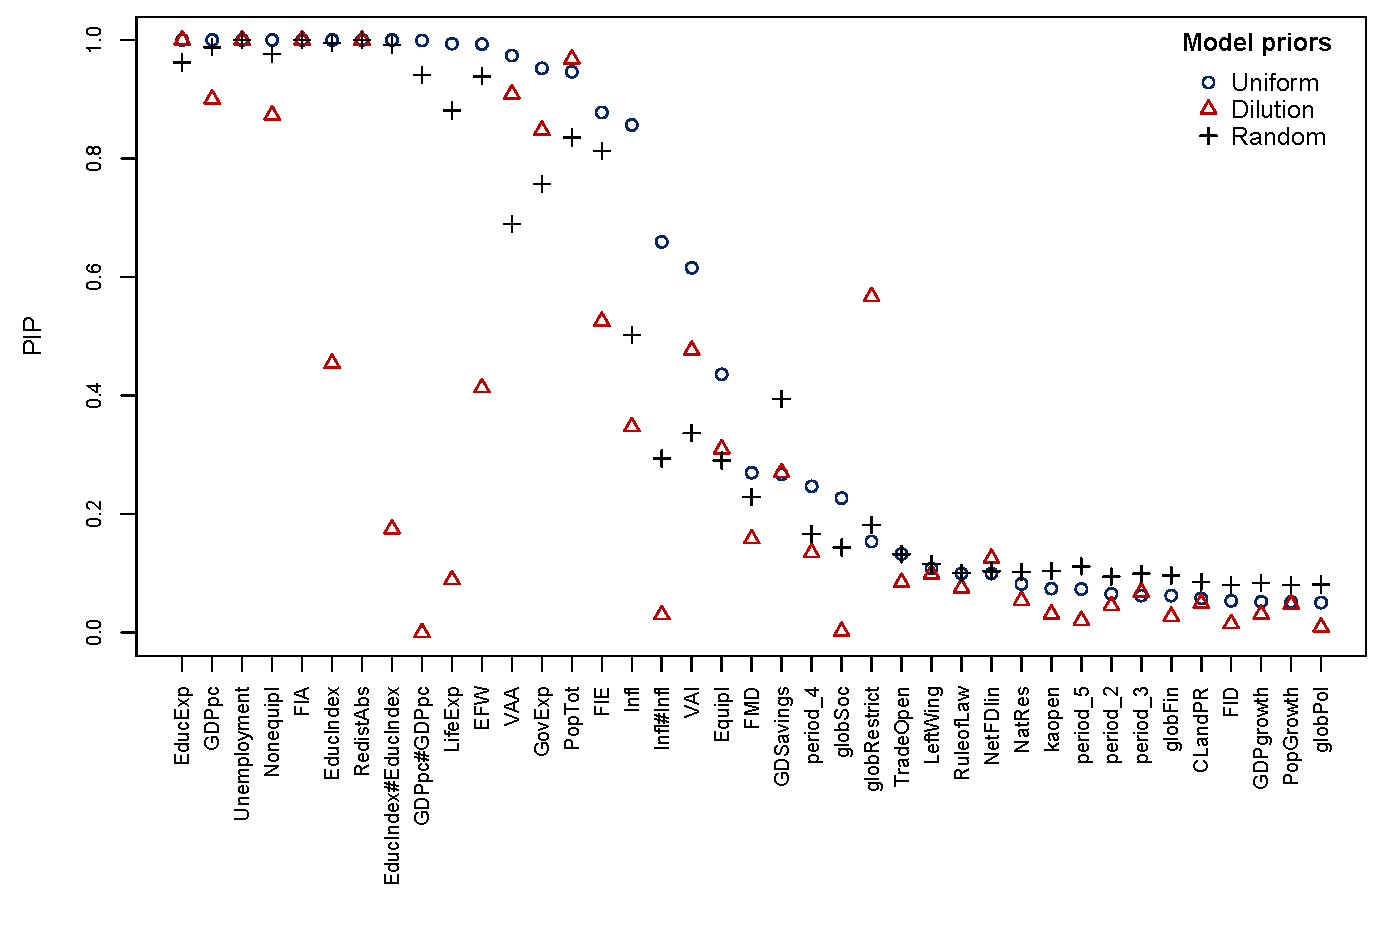
\includegraphics[width=\textwidth, keepaspectratio]{figures/ch4/model_priors_comparison_gini}
\end{figure}

\begin{figure}[htbp!]
  \caption{Robustness checks with alternative model priors, Top 10
  \% share}
  \label{ch4fig:top10_comp}
  \centering
  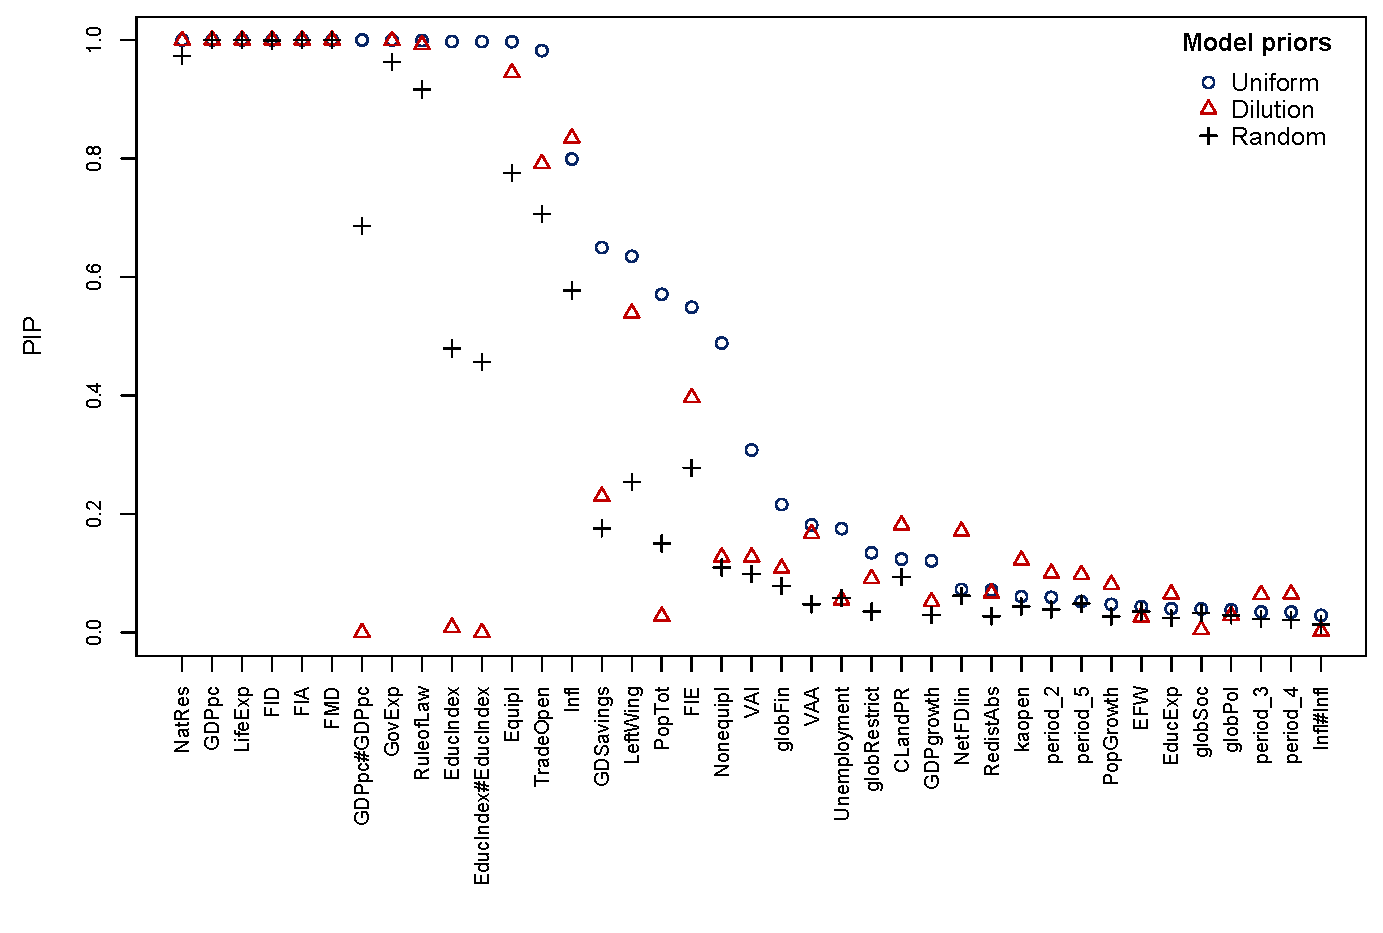
\includegraphics[width=\textwidth, keepaspectratio]{figures/ch4/model_priors_comparison_top10}
\end{figure}

\begin{figure}[htbp!]
  \caption{Robustness checks with alternative model priors, Top 1\% share}
  \label{ch4fig:top1_comp}
  \centering
  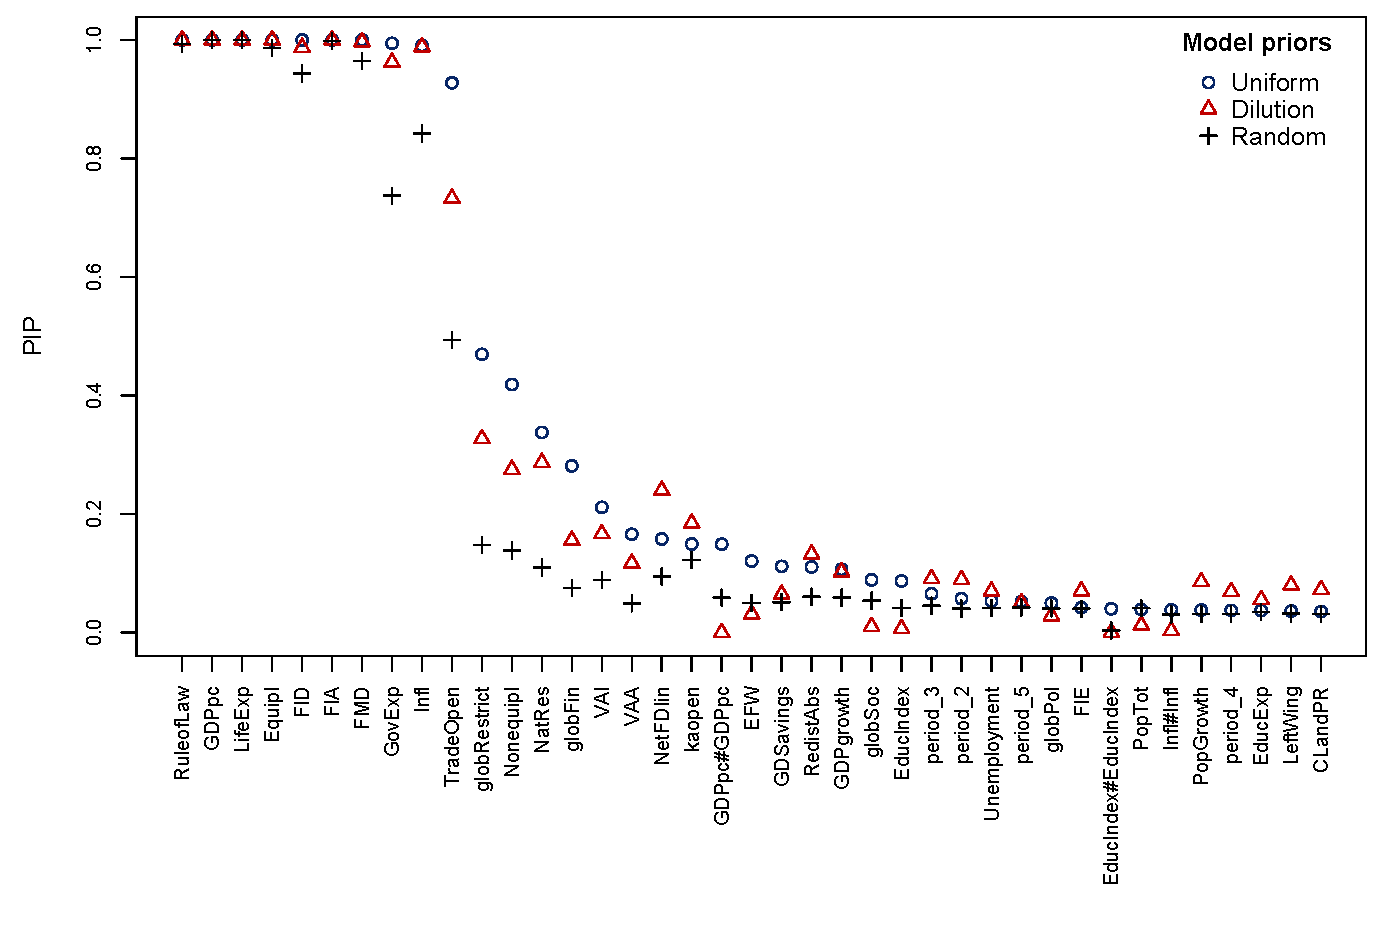
\includegraphics[width=\textwidth, keepaspectratio]{figures/ch4/model_priors_comparison_top1}
\end{figure}

\begin{figure}[htbp!]
  \caption{\acp{PIP} with different inequality measures}
  \label{ch4fig:comp_ineq_sel}
  \centering
  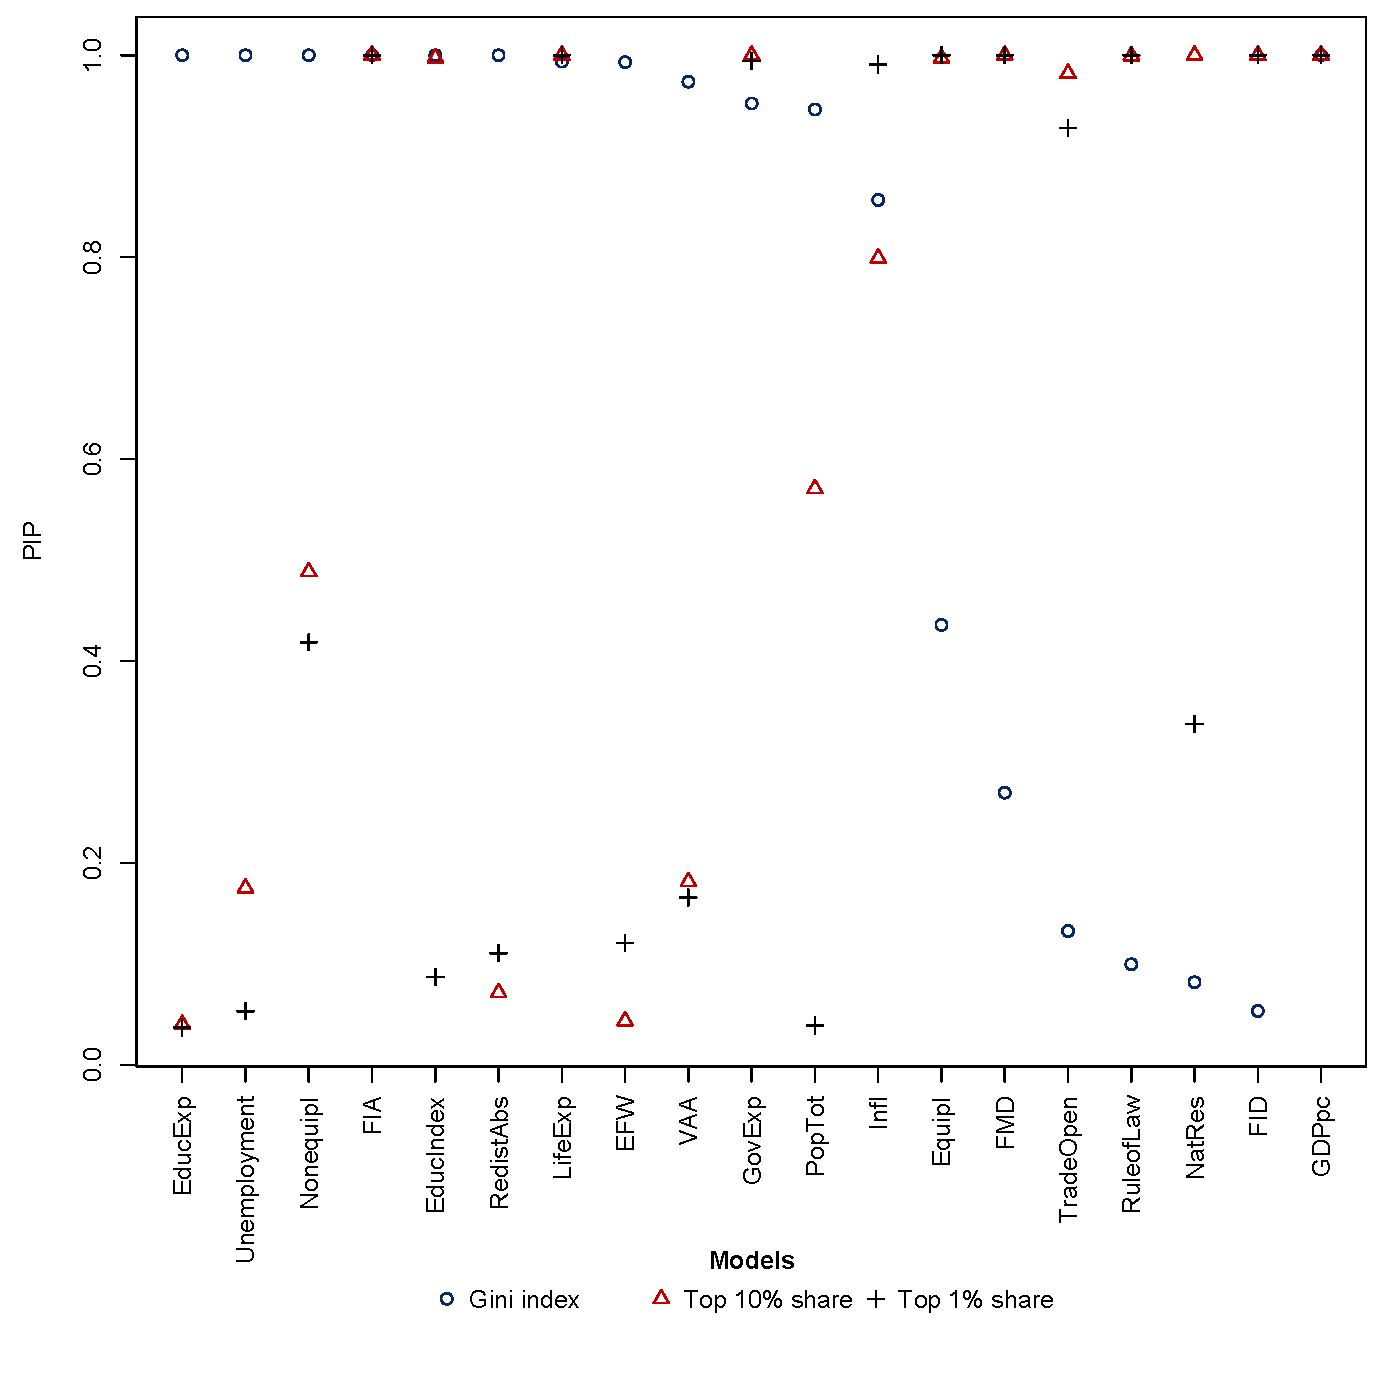
\includegraphics[width=0.8\textwidth, keepaspectratio]{figures/ch4/comp_baseline_pip_sel}

  \begin{minipage}{0.8\textwidth}
    \footnotesize
    \emph{Note: The comparison only shows variables which show \ac{PIP} $> 0.9$ in at least one of the models.}
    \end{minipage}
\end{figure}

\begin{figure}[htbp!]
  \caption{\acp{PIP} for different top income shares with baseline priors}
  \label{ch4fig:comp_topshares}
  \centering
  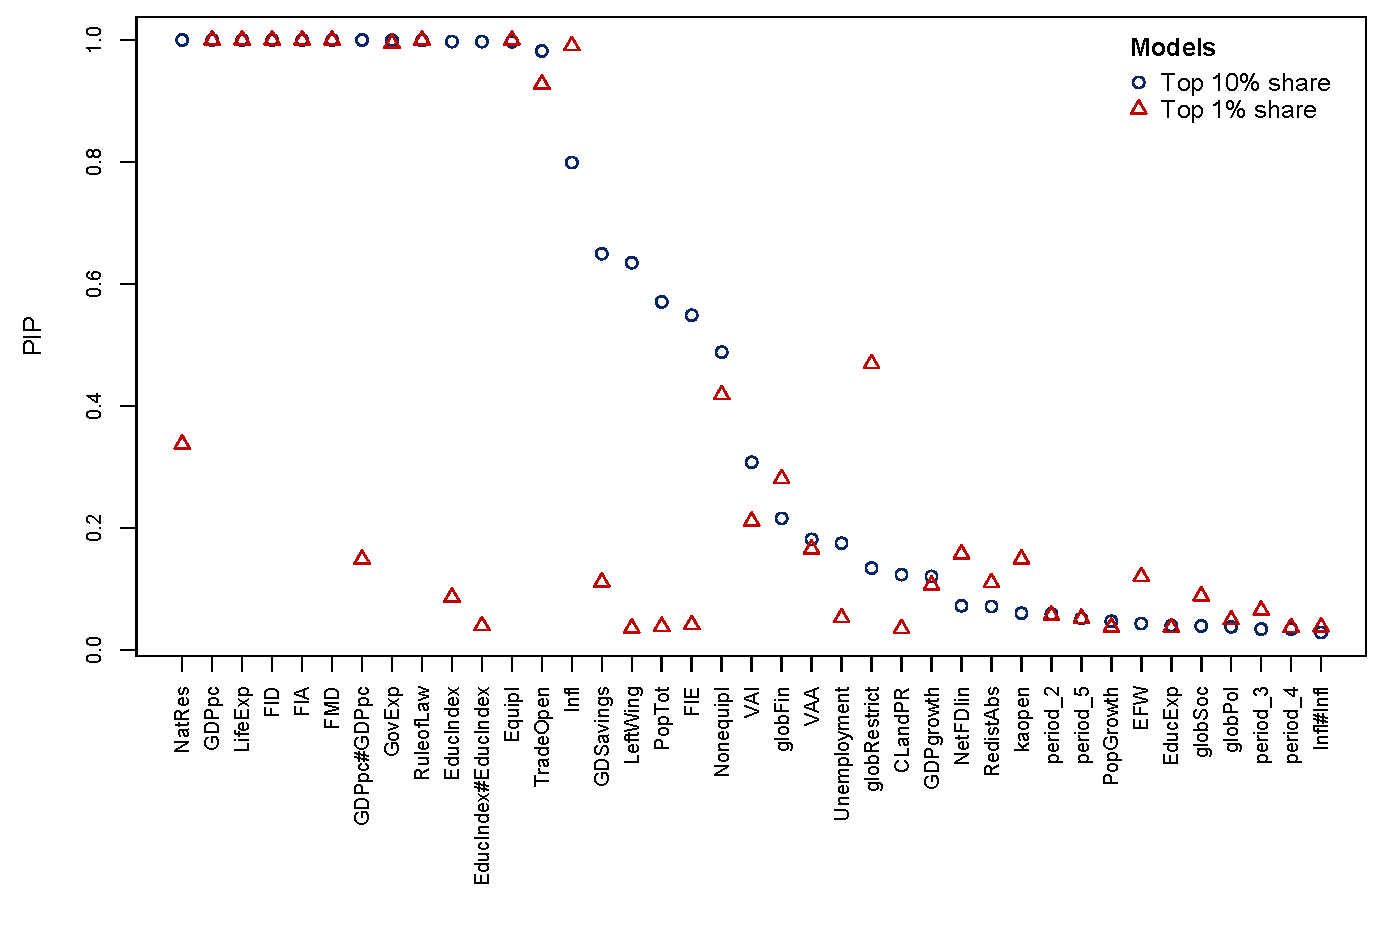
\includegraphics[width=\textwidth, keepaspectratio]{figures/ch4/topsh_comparison_all}
  \begin{minipage}{0.8\textwidth}
    \footnotesize
    \emph{Note: Random note. This figure might not be included in the end.}
    \end{minipage}
\end{figure}

\begin{table}[htbp!]
  \caption{BMA, baseline results. Dependent variable after-tax Gini index, 394 observations.}\label{ch4res:baseline_gini}
  \footnotesize
  \centering
  \begin{tabular}{lrrr}
    \toprule
                           & PIP & Post Mean & Post SD \\
    \midrule
    Education expenditures & 1.00 & -0.14506 & 0.05042 \\
  GDP per capita & 1.00 & 1.62811 & 0.56870 \\
  Unemployment & 1.00 & 0.23629 & 0.05907 \\
  Non-equipment investment & 1.00 & 0.14977 & 0.05285 \\ 
  Access to financial institutions & 1.00 & -0.24629 & 0.06342 \\
  Education index (UN) & 1.00 & -0.58853 & 0.23865 \\ 
  Redistribution & 1.00 & -0.22055 & 0.05051 \\
  Education index sq. & 1.00 & 0.82252 & 0.22008 \\
  GDP per capita sq. & 1.00 & -1.44906 & 0.57565 \\
  Life expectancy & 0.99 & -0.22879 & 0.09750 \\ 
  Economic freedom & 0.99 & 0.18518 & 0.06941 \\
  Value added in agriculture & 0.97 & -0.12361 & 0.05947 \\
  Government expenditures & 0.95 & 0.12259 & 0.05743 \\ 
  Total population & 0.95 & -0.15378 & 0.08478 \\
  Financial institutions efficiency & 0.88 & -0.08374 & 0.05599 \\
  Inflation & 0.86 & 0.16879 & 0.12487 \\
  \midrule
  Inflation sq. & 0.66 & -0.11127 & 0.11201 \\ 
  Value added in industry & 0.62 & -0.05825 & 0.06407 \\
  Equipment investment & 0.44 & -0.03383 & 0.05359 \\ 
  Financial markets depth & 0.27 & 0.01554 & 0.03673 \\ 
  Gross domestic savings & 0.27 & -0.02022 & 0.04597 \\
  % Period 4 & 0.25 & 0.01282 & 0.03330 \\ 
  Social globalization & 0.23 & 0.02365 & 0.06279 \\
  Restrictions on globalization & 0.15 & 0.00874 & 0.03214 \\
  Trade openness & 0.13 & 0.00615 & 0.02589 \\
  Left-wing orientation & 0.11 & 0.00339 & 0.01720 \\ 
  Rule of law & 0.10 & -0.00333 & 0.01812 \\ 
  Net FDI (\% GDP) & 0.10 & -0.00283 & 0.01575 \\ 
  Natural resources rents & 0.08 & -0.00223 & 0.01583 \\ 
  Chinn-Ito index & 0.07 & -0.00205 & 0.01780 \\ 
  % Period 5 & 0.07 & 0.00025 & 0.02188 \\ 
  % Period 2 & 0.07 & 0.00133 & 0.01321 \\
  % Period 3 & 0.06 & -0.00027 & 0.01423 \\
  Financial globalization & 0.06 & -0.00134 & 0.01466 \\
  Civil liberties \& political rights & 0.06 & 0.00075 & 0.01131 \\ 
  Financial institutions depth & 0.05 & 0.00060 & 0.01316 \\ 
  GDP growth & 0.05 & 0.00016 & 0.01255 \\
  Population growth & 0.05 & 0.00055 & 0.01052 \\ 
  Political globalization & 0.05 & 0.00000 & 0.01432 \\  
    \bottomrule
  \end{tabular}
  \end{table}

\begin{table}[htbp!]
  \caption{BMA, baseline results. Dependent variable Top 10\% share, 394 observations.}\label{ch4res:baseline_top10}
    \footnotesize
    \centering
  \begin{tabular}{lrrr}
      \toprule
                              & PIP & Post Mean & Post SD \\
      \midrule
  Natural resources rents & 1.00 & -0.15595 & 0.04773 \\
  GDP per capita & 1.00 & 2.13915 & 0.54791 \\
  Life expectancy & 1.00 & -0.53327 & 0.09806 \\
  Financial institutions depth & 1.00 & 0.20288 & 0.05638 \\
  Access to financial institutions & 1.00 & -0.25218 & 0.06712 \\
  Financial markets depth & 1.00 & 0.19376 & 0.04976 \\
  GDP per capita sq. & 1.00 & -1.80042 & 0.55408 \\ 
  Government expenditures & 1.00 & 0.15638 & 0.05565 \\ 
  Rule of law & 1.00 & -0.12607 & 0.04665 \\
  Education index (UN) & 1.00 & -0.49573 & 0.22152 \\ 
  Education index sq. & 1.00 & 0.58180 & 0.20423 \\
  Equipment investment & 1.00 & -0.13953 & 0.05578 \\ 
  Trade openness & 0.98 & 0.12632 & 0.05604 \\
  Inflation & 0.80 & 0.06758 & 0.05407 \\ 
  \midrule
  Gross domestic savings & 0.65 & 0.06566 & 0.06764 \\
  Left-wing orientation & 0.63 & 0.04567 & 0.04858 \\ 
  Total population & 0.57 & 0.07224 & 0.08621 \\ 
  Financial institutions efficiency & 0.55 & -0.04309 & 0.05278 \\
  Non-equipment investment & 0.49 & 0.03864 & 0.05320 \\ 
  Value added in industry & 0.31 & -0.02652 & 0.05253 \\
  Financial globalization & 0.22 & -0.01390 & 0.03673 \\ 
  Value added in agriculture & 0.18 & -0.01163 & 0.03405 \\ 
  Unemployment & 0.18 & -0.01019 & 0.03113 \\
  Restrictions on globalization & 0.13 & 0.00637 & 0.02398 \\ 
  Civil liberties \& political rights & 0.12 & 0.00529 & 0.02137 \\
  GDP growth & 0.12 & 0.00608 & 0.02464 \\ 
  Net FDI (\% GDP) & 0.07 & -0.00217 & 0.01377 \\ 
  Redistribution & 0.07 & -0.00243 & 0.01571 \\
  Chinn-Ito index & 0.06 & 0.00170 & 0.01373 \\ 
  % Period 2 & 0.06 & -0.00160 & 0.01267 \\
  % Period 5 & 0.05 & 0.00158 & 0.01431 \\ 
  Population growth & 0.05 & 0.00097 & 0.01043 \\
  Economic freedom & 0.04 & 0.00055 & 0.01416 \\ 
  Education expenditures & 0.04 & -0.00062 & 0.01030 \\
  Social globalization & 0.04 & -0.00004 & 0.01918 \\ 
  Political globalization & 0.04 & 0.00060 & 0.01279 \\
  % Period 3 & 0.03 & -0.00007 & 0.00873 \\ 
  % Period 4 & 0.03 & -0.00017 & 0.00827 \\
  Inflation sq. & 0.03 & -0.00045 & 0.01581 \\
  \bottomrule
  \end{tabular}
\end{table}

\begin{table}[htbp!]
  \caption{BMA, baseline results. Dependent variable Top 1\% share, 394 observations.}\label{ch4res:baseline_top10}
    \footnotesize
    \centering
  \begin{tabular}{lrrr}
    \toprule
                                 & PIP & Post Mean & Post SD \\
    \midrule
  Rule of law & 1.00 & -0.17039 & 0.04688 \\
  GDP per capita & 1.00 & 0.48163 & 0.29090 \\
  Life expectancy & 1.00 & -0.45605 & 0.06980 \\
  Equipment investment & 1.00 & -0.19727 & 0.05526 \\
  Financial institutions depth & 1.00 & 0.16380 & 0.05689 \\ 
  Access to financial institutions & 1.00 & -0.25945 & 0.06419 \\
  Financial markets depth & 1.00 & 0.15454 & 0.04989 \\ 
  Government expenditures & 0.99 & 0.11633 & 0.04718 \\ 
  Inflation & 0.99 & 0.11773 & 0.04922 \\
  Trade openness & 0.93 & 0.10374 & 0.05711 \\ 
  \midrule
  Restrictions on globalization & 0.47 & 0.03804 & 0.05418 \\ 
  Non-equipment investment & 0.42 & 0.03197 & 0.05001 \\ 
  Natural resources rents & 0.34 & -0.02182 & 0.04037 \\ 
  Financial globalization & 0.28 & -0.02001 & 0.04269 \\
  Value added in industry & 0.21 & -0.01389 & 0.03634 \\
  Value added in agriculture & 0.17 & -0.00969 & 0.03053 \\ 
  Net FDI (\% GDP) & 0.16 & -0.00730 & 0.02401 \\
  Chinn-Ito index & 0.15 & 0.00828 & 0.02797 \\
  GDP per capita sq. & 0.15 & -0.08401 & 0.28484 \\
  Economic freedom & 0.12 & -0.00945 & 0.03762 \\ 
  Gross domestic savings & 0.11 & 0.00634 & 0.02688 \\
  Redistribution & 0.11 & 0.00495 & 0.02085 \\
  GDP growth & 0.11 & -0.00504 & 0.02208 \\
  Social globalization & 0.09 & -0.00626 & 0.03233 \\
  Education index (UN) & 0.09 & -0.01003 & 0.07309 \\ 
  % Period 3 & 0.07 & -0.00214 & 0.01452 \\
  % Period 2 & 0.06 & -0.00146 & 0.01249 \\
  Unemployment & 0.05 & 0.00131 & 0.01287 \\ 
  % Period 5 & 0.05 & 0.00140 & 0.01362 \\
  Political globalization & 0.05 & 0.00137 & 0.01473 \\ 
  Financial institutions efficiency & 0.04 & -0.00070 & 0.01024 \\ 
  Education index sq. & 0.04 & 0.01380 & 0.07857 \\ 
  Total population & 0.04 & -0.00060 & 0.01484 \\ 
  Inflation sq. & 0.04 & 0.00053 & 0.01828 \\ 
  Population growth & 0.04 & 0.00020 & 0.00844 \\
  % Period 4 & 0.04 & 0.00019 & 0.00892 \\ 
  Education expenditures & 0.04 & -0.00002 & 0.00935 \\ 
  Left-wing orientation & 0.04 & -0.00028 & 0.00843 \\ 
  Civil liberties \& political rights & 0.04 & 0.00009 & 0.00846 \\
    \bottomrule
  \end{tabular}
\end{table}

\textcite{kroszneretal2007} show that financial crises have relative more severe impact on the sectors which depend more on external financing. The consequences of crises on firms relate to institutional environment and materialize through lower production capacity and competition.

\section{Conclusion}
\label{ch4sec:conclusion}
Overall, these results suggest that policies seeking to improve the governance and robustness of local banks should be prioritized over size-enhancing reforms from a normative point of view \parencite{gimet2011closer}.
\clearpage
%
%
%
%
%
\printbibliography
\addcontentsline{toc}{section}{Bibliography}
%
%
%
%
%
\clearpage
%
% \appendix
\section*{Appendix}
\label{ch4sec:appch2}
\begin{subappendices}
\subsection{The composition of financial indicators}
\label{ch4subsec:finind_comp}
\begin{table}[ht!]
    \small
    \caption{Underlying Components of Financial Development Indicators}
    \label{ch4tab:finind}
    \centering
    \begin{tabular}{ll}
      \toprule
      \textsc{Indicator} & \textsc{Measure} \\
      \midrule
      \multicolumn{2}{l}{\textbf{Financial institutions}} \\
      \midrule
      \multirow{2}{*}{Access} 	& Bank branches per 100,000 adults \\
                                  & ATMs per 100,000 adults \\
      \midrule
      \multirow{6}{*}{Efficiency}		& Net interest margin \\
                                  & Lending-deposits spread \\ 
                                  & Noninterest income to total income \\
                                  & Overhead costs to total assets \\
                                  & Return on assets \\
                                  & Return on equity \\
            
      \midrule
      \multirow{4}{*}{Depth}	& Domestic private credit to the real sector to the GDP \\
                                  & Pension fund assets/GDP \\
                                  & Mutual fund assets/GDP \\
                                  & Insurance premiums life and nonlife/GDP \\
      \midrule
      \multicolumn{2}{l}{\textbf{Financial markets}} \\
      \midrule
      \multirow{6}{*}{Depth} 	& Stock market capitalization/GDP \\
                                  & Stocks traded/GDP \\
                                  & International debt securities of government/GDP \\
                                  & Total debt securities of financial corporations/GDP \\
                                  & Total debt securities of nonfinancial corporations/GDP \\
      \midrule
      Efficiency                  & Stock market turnover ratio (stocks traded/capitalization) \\
      \bottomrule
    \end{tabular}
\end{table}

\clearpage
\subsection{Dataset description}
\begin{center}
\footnotesize
\begin{longtable}{l p{0.50\linewidth} p{0.3\linewidth}}
    \caption{List of variables}
    \label{ch4app:exog} \\
    \toprule 
  Variable & Definition (+ optional comments) & Source \\
    \midrule 
  GiniNet & After\-tax Gini index based on distribution of income (The Standardized World Income Inequality Database). & \href{http://fsolt.org/swiid/}{Solt (2019)} \\
  GiniMarket & Before-tax Gini index based on distribution of income  (The Standardized World Income Inequality Database). & \href{http://fsolt.org/swiid/}{Solt (2019)} \\	
  Top10share & Share of income going top decile of the distribution. & \href{https://wid.world/}{WID} \\	
  Top1share & Share of income going top percentile of the distribution. & \href{https://wid.world/}{WID} \\
  FIA & Access to financial institutions & \href{http://data.imf.org/?sk=F8032E80-B36C-43B1-AC26-493C5B1CD33B}{\textcite{svirydzenka2016introducing}} \\
  FID & Financial institutions depth & \href{http://data.imf.org/?sk=F8032E80-B36C-43B1-AC26-493C5B1CD33B}{\textcite{svirydzenka2016introducing}} \\
  FIE & Financial institutions efficiency & \href{http://data.imf.org/?sk=F8032E80-B36C-43B1-AC26-493C5B1CD33B}{\textcite{svirydzenka2016introducing}} \\
  FMD & Financial markets depth & \href{http://data.imf.org/?sk=F8032E80-B36C-43B1-AC26-493C5B1CD33B}{\textcite{svirydzenka2016introducing}} \\
  FME & Financial markets efficiency & \href{http://data.imf.org/?sk=F8032E80-B36C-43B1-AC26-493C5B1CD33B}{\textcite{svirydzenka2016introducing}} \\
  GDPpc & Level of GDP per capita & \href{http://data.worldbank.org/indicator/NY.GDP.PCAP.PP.KD}{WB} \\
  NatRes & Total natural resource rents are the sum of oil rents, natural gas rents, coal rents (hard and soft), mineral rents, and forest rents. & \href{http://data.worldbank.org/indicator/NY.GDP.TOTL.RT.ZS}{WB} \\
  PopGrowth & Annual population growth 1980-2009 & \href{http://data.worldbank.org/indicator/SP.POP.GROW}{WB} \\
  GovExp & General government final consumption expenditure (formerly general government consumption). & \href{http://data.worldbank.org/indicator/NE.CON.GOVT.ZS}{WB}\\
  NNSavings & Net national savings (gross national savings less the value of consumption of fixed capital, \% GNI). & \href{http://data.worldbank.org/indicator/NY.ADJ.NNAT.GN.ZS}{WB} \\
  EducExp & Education expenditure refers to the current operating expenditures in education, including wages and salaries and excluding capital investments in buildings and equipment.. & \href{http://data.worldbank.org/indicator/NY.ADJ.AEDU.GN.ZS}{WB} \\
  Infl & Inflation as measured by the consumer price index. & \href{http://data.worldbank.org/indicator/FP.CPI.TOTL.ZG}{WB} \\
  VAA & Agriculture, forestry, and fishing value added (\% GDP). & \href{http://data.worldbank.org/indicator/NV.AGR.TOTL.ZS}{WB} \\
  VAI & Industry value added (\% GDP). & \href{http://data.worldbank.org/indicator/NV.IND.TOTL.ZS}{WB} \\
  GFCF & Gross fixed capital formation (\% of GDP). & \href{http://data.worldbank.org/indicator/NE.GDI.FTOT.ZS}{WB} \\
  NetFDI &  Foreign direct investment, net inflows (\% of GDP). & \href{http://data.worldbank.org/indicator/BX.KLT.DINV.WD.GD.ZS}{WB} \\
  GDPgrowth & Annual growth of GDP. & \href{http://data.worldbank.org/indicator/NY.GDP.MKTP.KD.ZG}{WB} \\
  LifeExp & Life expectancy at birth.  & \href{http://data.worldbank.org/indicator/SP.DYN.LE00.IN}{WB}\\
  LabForce & Total labor force comprises people ages 15 and older who meet the International Labor Organization definition of the economically active population: all people who supply labor for the production of goods and services during a specified period. Labor force total. & \href{http://data.worldbank.org/indicator/SL.TLF.CACT.ZS}{WB} \\
%   PopDens & Population density (people per sq. km of land area). & \href{http://data.worldbank.org/indicator/EN.POP.DNST}{WB} \\
  RuleOfLaw & Rule of law estimate & \href{http://data.worldbank.org/indicator/RL.EST}{WB} \\
  CLandPR & Average of index for civil liberties and political rights & \href{https://freedomhouse.org/report/freedom-world-2016/methodology}{Freedom House} \\
%   OutwardO & Trade (\% of GDP)  & \href{http://data.worldbank.org/indicator/NE.TRD.GNFS.ZS}{WB} \\
  ChinnIto & Chinn-Ito index of financial openness. & \href{http://web.pdx.edu/~ito/Chinn-Ito_website.htm}{Chinn-Ito} \\ 
  LeftWing & Dummy equal to 1 when left oriented party lead the country. & \href{http://www.nsd.uib.no/macrodataguide/set.html?id=11&sub=1}{DPI} \\
  ActivRestrict & Activity restrictions. Regulatory restrictions on bank activities and the mixing of banking and commerce. & \href{http://faculty.haas.berkeley.edu/ross_levine/regulation.htm}{Barth et al. (2013)} \\
  CapitalReg & Capital Regulatory index. & \href{http://faculty.haas.berkeley.edu/ross_levine/regulation.htm}{Barth et al. (2013)} \\
  DiversIndex & Whether there are explicit, verifiable, quantifiable guidelines for asset diversification and banks are allowed to make loans abroad. & \href{http://faculty.haas.berkeley.edu/ross_levine/regulation.htm}{Barth et al. (2013)} \\
  EducIndex & Calculated using mean years of schooling and expected years of schooling & \href{http://hdr.undp.org/en/content/education-index}{UN} \\
  NetInterestMargin & Accounting value of banks' net interest revenue as a share of average interest-bearing assets; a measure of the efficiency of the banking sector. & \href{http://data.worldbank.org/data-catalog/global-financial-development}{GFDD} \\
  BankZScore & return on banks' assets plus the ratio of banks' equity and assets, divided by the standard deviation of the return on assets (ROA+equity/assets)/sd(ROA); a measure of stability of the banking sector & \href{http://data.worldbank.org/data-catalog/global-financial-development}{GFDD} \\
  Privatecredit & Domestic private credit to the real sector to GDP; a measure of the depth of the banking sector & \href{http://data.worldbank.org/data-catalog/global-financial-development}{GFDD} \\
  MarketCap & Value of listed shares to GDP; a measure of the depth of stock markets.& \href{http://data.worldbank.org/data-catalog/global-financial-development}{GFDD} \\
  MarketTurn & Stock market value traded to total market capitalization; a measure of the efficiency of stock markets. & \href{http://data.worldbank.org/data-catalog/global-financial-development}{GFDD} \\
  BankBranches & Number of bank branches per 100,000 adults & \href{http://data.worldbank.org/data-catalog/global-financial-development}{GFDD} \\
  Loan2Deposits & Loan-to-deposit ratio. & \href{http://data.worldbank.org/data-catalog/global-financial-development}{GFDD} \\
  Redist & Difference between market (pre-tax) and net (after-tax0 Gini index based on distribution of income  (The Standardized World Income Inequality Database). & \href{http://fsolt.org/swiid/}{Solt (2016)} \\	
  FinLib & Averaged components of Economic Freedom of the World index 3D (freedom to own foreign currency accounts), 4C (black-market exchange rates), 4D (controls of the movement of capital and people), and 5A (credit market regulations). & \href{https://www.fraserinstitute.org/economic-freedom/dataset}{\textcite{gwartney2017}} \\
  \bottomrule
\end{longtable}
\end{center}

\end{subappendices}
\end{refsection}
% \chapter{Title of Chapter Five}
\label{chap:five}

\section{Title of Section One}

The following checklist should help in avoiding some frequently made mistakes, if any of the following propositions apply for your thesis, there is a problem:

\begin{itemize} 
		\item You have citations in your abstract.
		\item The introduction does not cover the three parts as described in \autoref{chap:one}.
		\item The introduction contains subheadings.
		\item You described different aspects than promised in the title.
		\item You copied some parts of the text from other work without proper referencing and citing.
		\item You used automatic translation tools to produce text by translating it from another language.
		\item Your thesis contains many typos and grammatical errors. (Use an electronic spell checker. Please!)
		\item You used color in your figures and refer to the ``blue'' line (assume that your readers use a monochrome printer).
		\item You mainly used websites and other unrefereed material as your sources or you used Wikipedia as your source.
		\item You refer to something in your conclusion which you have not mentioned before.
		\item Some forenames in the references are abbreviated, some not.
		\item Some references miss a publishing date.
\end{itemize}



% \chapter{Useful Hints}
\label{chap:six}

If you write in English, you might find the following hint
useful: The indefinite article a is used as an before a
vowel sound---for example an apple, an hour, an unusual
thing, an \ac{MNC} (because the acronym is pronounced Em-En-See). Before a consonant sound represented
by a vowel letter a is usual---for example a one, a
unique thing, a historic chance. Few more tips to follow:


\begin{itemize}
\item Don't give orders---don't write in the imperative mood---unless you are training to be a teacher.
\item Avoid the use of questions. You may know the answer: does your reader? It's much safer to tell her, or him.
\item Do not become entangled in the problems of `sexist' language. It is much easier to write in the plural. ``Students should check their work'' is good English. ``A student should check---'' is also good English, but now the problems begin: ``---her work?'' ``---his work?'' Which? You can write ``his or her,'' but that seems clumsy. Stick to the plural.
\item If you must refer to yourself, use the third person such as ``The present writer would recommend that \ldots'' may be useful.
\item Use the full forms of words and phrases, not contractions like ``he's,'' ``don't,'' etc. Keep the apostrophe to indicate possession---and use it correctly. Academics really sneer at students who use the ``Greengrocer's apostrophe.''
\end{itemize}


\begin{itemize}
\item Do not despise short, workmanlike, and effective plain English words. If they mean what you want to say. Accurately.
\item Avoid the use of humor in academic writing---unless you are very sure of yourself.
\item Even when you are not being funny, avoid the use of irony or sarcasm.
\item Paragraphs in academic English should contain more than one sentence. (Short paragraphs look as if you are writing for a tabloid newspaper---or a simple Template!) I guess that the average academic book runs to two or three paragraphs per page. Look at the books in your subject, and get a feel for how long your own paragraphs should be when you are imitating the academic style.
\item Use the word that more in formal writing than most of us do in speech---particularly after such verbs of utterance as to say, to report, to think etc. It can help to make your writing much clearer.
\item Develop an academic vocabulary. The `long words' you learn in the course of your studies are long usually because they have more precise meanings than their less formal equivalents. They are therefore better when you want to be accurate. (Also they allow you to sound like someone who deserves a degree.)
\end{itemize}



\begin{itemize}
\item  Use as few words as you can; but use enough words to express your meaning as fully as you can. Your judgment of what is appropriate here is part of what you should learn throughout your course.
\item  Avoid lazy words such as ``nice''. It is usually better to say ``acquire'' or ``obtain'' than ``get;'' and it may be better, if you mean ``through the use of money,'' to say ``purchase'' or---better still---''buy.''
\item A short word like ``buy'' is better than a long one like ``purchase''---unless the long one is more accurate. A ``statutory instrument'' is better than a ``rule''---to a lawyer, at any rate.
\item Proof-read with care. Ask someone else to help---you may be too close to your work to be able to see your mistakes.
\item If in doubt, choose the more formal, or possibly just the more old-fashioned, of two words. For example, say quotation rather than quote whenever you mean the use of somebody else's words.
\end{itemize}



\begin{itemize}
\item You will often sound more academic if you include doubts in your work---and qualifications. Within the scope of this thesis, the current writer cannot hope to cover all the possible implications of the question.ԍ
\item In this context, the use of litotes sounds very academic. This is the construction where a writer uses a negative with a negative adjective, e.g.\ it is not unlikely that \ldots This does not mean the same as it is probable that \ldots It has a shade of meaning and qualification that can be useful to academic writers.
\end{itemize}





% \chapter{Conclusion}
\label{conclusion}

The conclusion should briefly summarize the problem statement and the general content of the work and the emphasize on the main contribution of the work.

When writing the conclusion keep in mind that some readers may not have gone through the whole thesis, but have jumped directly to the conclusion after having read the abstract in order the decide on the personal relevance of the thesis. Therefore, the conclusion should be self contained, which means that a reader should be able to understand the essence of the conclusion without having to read the whole thesis.

The conclusion typically ends with an outlook that describes possible extensions of the presented approaches and of planned future work.

\begin{refsection}
\clearpage
%-----<<< -------- >>>-----

%-----<<< REFERENCES >>>-----
% \fancyhead[LO]{\sffamily Bibliography}					%headers in sans serif and not in uppercase
% \bibliographystyle{Styles/Stylebib}							%style of literature, you can use e.g. newapa	instead of Styles/Stylebib
% \bibliography{Styles/literature}							%bibliography database
% \addcontentsline{toc}{chapter}{Bibliography} 		%Add bibliography to the table of contents
% \clearpage
%-----<<< ---------- >>>-----

%-----<<< APPENDIXES >>>-----
\backmatter																			%uppercase roman pagination for back matter; appendices start
\autohdr																				%automatic headers     				
% \chapter{Response to the referees}
\section{Doc. PhDr. Adam Ger\v{s}l Ph.D.}

\textbf{\textit{Comments to the first paper on ``What Type of Finance Matters for Growth? Bayesian Model Averaging Evidence''}}

% {\itshape The dissertation thesis is a collection of three very well written empirical papers exploring the links between financial development on one hand and long-term economic growth, wealth inequality, and income inequality on the other hand. The author demonstrates strong skills in using up-to-date econometric methods, especially the Bayesian Model Averaging (BMA), to analyze available data on relevant economic phenomena. The first paper titled ``What Type of Finance Matters for Growth? Bayesian Model Averaging Evidence'' explores the finance-growth link with an updated dataset on long-term per capita GDP growth, a number of economic and institutional factors, and selected variables capturing financial intermediation. The value added is in using the BMA framework to account for model uncertainty and in testing the explanatory power of five selected financial development indicators: in addition to the traditional credit to GDP and stock market capitalization (both capturing the depth of financial intermediation), the paper uses a measure of bank efficiency (net interest margin), a measure of stock market activity (turnover rate), and a measure of bank stability (the Z-score). The author finds that especially the bank efficiency measure is robustly related to long-term economic growth, which much higher inclusion probability than the traditional financial depth indicators.

% The second paper on ``Finance and Wealth Inequality'' uses the BMA framework to explore the link between financial, economic and institutional factors and the wealth Gini coefficient for a sample of 73 countries. The results show that finance has a multi-faced impact on wealth inequality – financial depth increases inequality, but efficiency and access to finance decrease it.

% The final paper investigates the link between financial intermediation and income inequality within a panel BMA framework. Also this paper finds that finance has a complex impact on inequality – the access to finance and efficiency decrease it, while the size of markets does not have any significant impact.

% There is an original contribution of the author in all three essays, all are based on relevant references, and all would be in my view defendable as a part of dissertation at respected universities. They are all written in a clear language and definitely publishable (actually, the first one has been published already in the World Bank Economic Review and the second in the Journal of International Money and Finance). While the focus is on data analysis and deriving relationships based on regression techniques, the thesis would benefit from a few revisions that would emphasize economic understanding, especially when interpreting the findings of the statistical exercises.

% My general assessment is that the thesis can be defended after revision indicated in my comments below.}

\begin{enumerate}
       
    \item \textit{The title is confusing - the paper does not explore what type of finance (bank versus market; bond versus stocks; banks versus non-bank institutions; short-term versus long-term; concentrated versus unconcentrated banking sector etc.) matters for growth, but what aspect of financial intermediation (financial depth; activity on markets; efficiency of banks; resilience of banks) matter. I propose to adjust the title accordingly.}
    
    Thank you for the valid point and a suggestion of an alternative. I changed the title of the first paper to \emph{What Aspect of Financial Intermediation Matters for Growth: Bayesian Model Averaging Evidence}. I adjusted the footnote referring to the publication of the chapter so that is reflects the title of the published paper.

    \item \textit{The endogeneity problem (briefly mentioned on p. 11) is much more serious than the author thinks as the variables get averaged over 50 years! The studies focusing on the dynamics of development between the real and financial sector (macrofinancial linkages, such as in Crowe et al. 2010) emphasize the two-way interactions and feedbacks that develop over time. As the methodology does not take into account the time dynamics, the thesis should at least acknowledge that endogeneity could be an issue and devote a paragraph or so to this shortcoming, adding a few references on the (omitted) dynamic interactions.}
    
    The point is well taken. Although the issue of endogeneity gets mentioned throughout the paper, it might come out as underappreciated. I have explicitly added a subsection discussing potential endogeneity and the limitations of our attempts to address it. While we can efficiently deal with the potential omitted variable bias by applying \ac{BMA}, the risk lies mainly in the reverse causality. To estimate where we use the lagged financial indicators and look at the shorter growth period, I added the results on the two-stage least squares \ac{BMA} that previously appeared in one of the footnotes and available upon request. Since finding the right instruments for our financial variables is a challenge, we focused this robustness exercise on the net interest margin as a measure of financial intermediation efficiency. Using the history of financial crises as an instrumental variable, we obtain results that support the baseline finding that intermediation efficiency is conducive to long-run growth.
    
    \item \textit{Throughout the paper, the net interest margin (NIM) is interpreted as a measure of ``efficiency of financial intermediaries'', but this is incorrect! It is a measure of (in)efficiencies in financial intermediation, not an indicator of bank (cost) efficiency! Large NIMs are typical for underdeveloped markets in which risks (of default), vulnerabilities, and legal uncertainties (of collateral realization etc.) are large, increasing information asymmetries and creating frictions to (efficient) financial intermediation. Thus, the NIM is actually an additional (indirect) measure of the institutional (legal) framework within which financial intermediation takes place rather than ``an aspect'' of financial activity.}

    Thank you for elaborating on this issue. Instead of adjusting the language throughout the first paper, I have added an introductory part in the summary of the dissertation about different approaches to the 'efficiency' in finance and how we understand it to be able to use efficiency of financial intermediaries interchangeably with the efficiency of financial intermediation. This also reflects one of the comments by Mr. \v{C}ih\'{a}k.

    \item \textit{Given the previous point, the author should be much more careful in drawing conclusions from the analysis. The fact that his measure of efficiency has a large PIP might be to a large extent related to the endogeneity bias: as an economy develops, the overall risks and vulnerabilities decline, contributing to a decline of the margin, which goes hand in hand with expansion in lending, further supporting economic development. This link should be mentioned in the paper.}    
    
    I partly address this comment in one of the related above. I have extended section devoted to discussing endogeneity. Although in a crude way, I tackle it in robustness check with lagged values of financial indicators similarly to the approach in the second paper on finance and wealth. The time span is shorter (10 years) and admittedly involves aftermath of financial crisis, but nevertheless, the conclusions are consistent with the baseline and it limits the mentioned risks to some extent. I agree that by averaging variables over long time spans, we lose information on the short-run dynamics and net interest margin may potentially mask effect of another variable. We attempt to avoid that by accounting for large volume of potential institutional factors explicitly in \ac{BMA} (rule of law, political rights, degree of capitalism, or openness of economy). In the 2SLS--BMA estimation, we include these potentially confounding factors in the first-stage regression.

    \item \textit{The review of literature mentions the criticism of traditional finance-growth nexus papers in neglecting the private bond markets (and other non-bank or non--stock--market sources of finance), but the paper again uses only the two traditional measures of financial depth -- bank credit and stock market (p. 10). Could the private credit to GDP be based on the BIS statistics of total credit (i.e. a sum of bank credit, non-bank intermediaries credit, bonds issues, and cross-border finance to private sector)? This has become available recently for a large number of countries (and years) and could better capture the debt of the private sector intermediated by all intermediaries and markets.}
    
    Thank you for pointing me to the \ac{BIS} data. Unfortunately, the coverage is insufficient to allow for using the data as is. Simply merging the data with our dataset reduces the number of observations to 33 and renders the baseline approach infeasible. Nevertheless, for the available data point, correlation between total credit and bank credit data is reaches nearly 0.7.(see also Figure \ref{app:total_bank_credit}). I have thus re-estimated the model with partially modified of total credit data from \ac{BIS}. I used the bank credit to non-financial sector data from \ac{GFDD} to estimate the total credit volumes for the countries with missing data. Next, I applied the \ac{BMA} using total credit instead of bank credit (and dropping the later from the set of covariates). Total credit shows low \ac{PIP} and none of the other relevant regressors is affected. Using the fitted values of total credit for all observations instead of only the missing values does not alter the results in any way. In Table \ref{chA:tab1} I only report \acp{PIP} along with the moments of the top covariates and total credit.
\end{enumerate}

\begin{figure}[ht!]
  \caption{Total vs. bank credit to non-financial sector}
  \label{app:total_bank_credit}
  \centering
  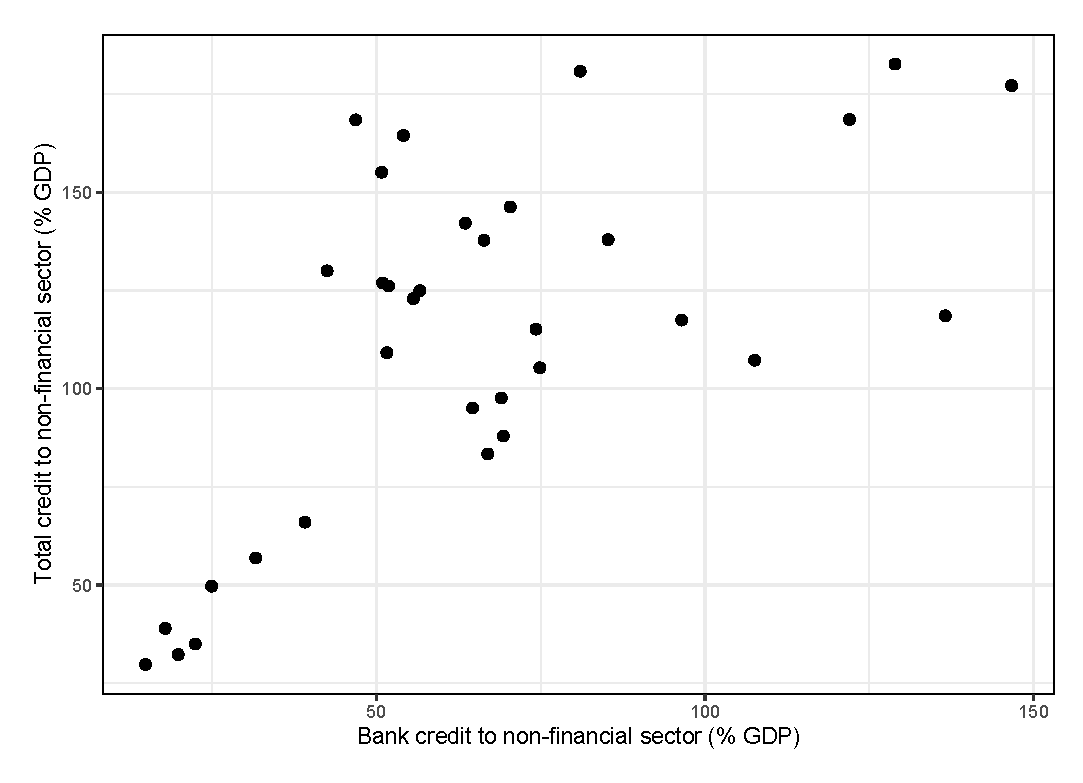
\includegraphics[width=0.8\textwidth, keepaspectratio]{figures/app/totalcredit_bankcredit}
\end{figure}

\begin{table}[ht!]
  \caption{Results total credit to non-financial institutions.}\label{chA:tab1}
    \footnotesize
    \centering
  \begin{tabular}{lrrr}
    \toprule
                                 & PIP & Post Mean & Post SD \\
    \midrule
    GDP level in 1960 & 1.00 & -0.01075 & 0.00241 \\
    Fraction GDP in mining & 1.00 & 0.04705 & 0.01344 \\
    Exchange rate distortions & 1.00 & -0.00009 & 0.00003 \\ 
    Fraction Confucian & 1.00 & 0.03898 & 0.01117 \\
    Life expectancy & 1.00 & 0.00058 & 0.00020 \\
    Fraction Buddhist & 0.99 & 0.01265 & 0.00495 \\ 
    Net interest margin & 0.96 & -0.00114 & 0.00047 \\ 
    Equipment investment & 0.83 & 0.07263 & 0.04768 \\
    \vdots \\
    \textbf{Total private credit} & 0.04 & 8.6345e-08 & 0.00001 \\
    \vdots \\
    \bottomrule
  \end{tabular}
\end{table}

\clearpage
\noindent \textbf{\textit{Comments to the second paper on ``Finance and Wealth Inequality''}}

\begin{enumerate}[resume]

    \item \textit{In comparison to the previous paper, this one tackles well a possible endogeneity bias (section 3.5.3) by lagging the explanatory variables (average of 1980-2009) compared to the dependent variable (average of 2010-2016), although I would be less concerned about the reverse link between inequality and financial development (compared to GDP growth and financial development). While a paragraph explaining through which channels would wealth inequality influence financial development is included on p. 66 (with reference to Beck et al. 2007), I am not too persuaded by (the two) explanations. Could 1-2 additional references be provided if, as the author states, ``the question of endogeneity is deeply ingrained in the finance-inequality nexus''? (Some additional arguments are included in the third paper and could be re-used here).}
    
    {\color{red}I have extended the discussion potential endogeneity by amending the text with additional references. - NEEDS TO BE DONE}
    
    \item \textit{In this paper, an overall index of efficiency is used, combining the net interest margin with variables such as overhead costs or profitability. I would still propose that this index is not called Financial Institutions Efficiency (but perhaps Financial Intermediation Efficiency) because it combines institutions' (cost) efficiency and efficiency (frictions) of financial intermediation influenced by overall risks. As this indicator has a 100\% PIP, it would be worth exploring further what drives the efficiency index -- is it more the NIM/spread as a measure of inefficiencies in financial intermediation (risks) or (overhead) costs as a measure of financial institutions' efficiency?}
    
    I took two different approaches in exploring the details of the FIE measure. First, the methodological paper to the financial development data by the IMF \parencite{svirydzenka2016introducing} provides the weights applied to the observed series to construct the indicator of financial intermediation efficiency. These are the loading factors in the principal component analysis which capture the common variation in the data related to the same category. This approach helps to correct for the overlapping information among multiple efficiency indicators and provides basis for their aggregation. In the case of FIE, the largest weight is on the overhead costs (25\%), net interest margin (20\%), lending-deposit spread, and non-interest income (both roughly 17\%). ROA and ROE both enter with relatively lower weights slightly above 10\%.

    Second approach relies on \ac{BMA} estimation with the underlying series of the FIE. I mirror the baseline methodological procedure using the individual indicators and report the results in Table \ref{chA:tab2}. The most important characteristics according the to \ac{PIP} are the overhead costs and net interest margin, both attaining values above 0.5. Both variables exhibit the expected positive posterior mean. The higher net interest margin and overhead costs relate to higher levels of wealth inequality as measured by Gini index. Unfortunately, I had to drop lending-deposit spread since the data was missing on part of the observations and the remaining components of intermediation efficiency show low inclusion probabilities.

    The procedure of the IMF and the estimate presented here thus show consistent results putting net interest margin and overhead costs upfront in capturing intermediation efficiency and its accompanying effects. Somewhat lower \acp{PIP} relative to the combined efficiency measure may arise from the collinearity between the individual indicators.
    
    \begin{table}[ht!]    
      \caption{Results using the individual components of financial intermediaries' efficiency}\label{chA:tab2}
      \centering
      \footnotesize
      \begin{tabular}{lrrr}
        \toprule
      Variable & PIP & Post Mean & Post SD \\
        \midrule
      Value added in agriculture & 1.00 & -0.53450 & 0.17265 \\
        Access to financial institutions & 0.99 & -0.38380 & 0.16285 \\ 
        Number of war years & 0.95 & 0.19154 & 0.10297 \\ 
        Outward orientation & 0.69 & 0.12387 & 0.11848 \\
        Economic freedom index (adjusted) & 0.66 & -0.22199 & 0.22503 \\ 
        Financial market depth & 0.60 & 0.25546 & 0.25381 \\
        \textbf{Net interest margin} & 0.57 & 0.22508 & 0.25392 \\ 
        \textbf{Overhead costs / Assets} & 0.56 & 0.16033 & 0.18376 \\ 
        Business conditions & 0.55 & -0.11950 & 0.14897 \\
        Financial institutions depth & 0.52 & 0.29136 & 0.33501 \\ 
        Inflation & 0.52 & 0.08456 & 0.10874 \\ 
        Education index (UN) & 0.51 & -0.15375 & 0.20071 \\
        Redistribution & 0.45 & -0.09356 & 0.13734 \\ 
        Net national savings & 0.30 & 0.04713 & 0.09898 \\
        Natural resources rents & 0.28 & 0.04244 & 0.09185 \\ 
        Labour market regulation & 0.26 & 0.03507 & 0.08022 \\
        Pre-tax ROA & 0.24 & -0.04709 & 0.12282 \\ 
        Net foreign direct investment & 0.23 & -0.02525 & 0.06581 \\
        Latin America dummy & 0.20 & 0.06632 & 0.20283 \\
        Financial openness (Chinn-Ito) & 0.14 & 0.01615 & 0.06855 \\
        Population density & 0.14 & -0.01313 & 0.05141 \\ 
        Rule of law & 0.13 & 0.02374 & 0.10437 \\
        Leftwing orientation & 0.12 & -0.00996 & 0.04222 \\ 
        Pre-tax ROE & 0.12 & 0.01714 & 0.07991 \\
        Banking diversification & 0.12 & -0.00837 & 0.03859 \\
        Public education expenditures & 0.12 & 0.00914 & 0.04335 \\ 
        Revolutions and coups & 0.11 & 0.00894 & 0.04639 \\
        Civ. liberties and Pol. rights & 0.10 & -0.01329 & 0.06491 \\
        Financial markets efficiency & 0.10 & 0.00863 & 0.04648 \\
        Financial liberalization (EFW) & 0.08 & 0.00169 & 0.05097 \\ 
        Life expectancy & 0.08 & -0.00032 & 0.06619 \\ 
        GDP level in 1990 & 0.08 & 0.00768 & 0.09478 \\
        Population growth & 0.08 & 0.00413 & 0.04553 \\
        Active banking restrictions & 0.07 & -0.00337 & 0.03223 \\ 
        Average GDP growth & 0.07 & -0.00390 & 0.03385 \\
        Bank capital regulations & 0.07 & -0.00426 & 0.02943 \\
        Non-interest income & 0.07 & 0.00133 & 0.03183 \\
        Technological progress & 0.06 & -0.00170 & 0.06215 \\ 
        Government expenditures & 0.06 & 0.00280 & 0.03468 \\
        Labour force participation & 0.06 & -0.00219 & 0.08291 \\
        Value added in industry & 0.05 & 0.00102 & 0.02998 \\ 
         \bottomrule
      \end{tabular}
      \end{table}

\noindent \textbf{\textit{Comments to the third paper on ``Finance and Inequality --- Panel BMA Approach''}}

    \item \textit{The paper could better formulate what is the value added compared to available literature. There are a few hints in the last paragraph on page 99, but this could be better structured and start with ``The value added of this paper is in \dots''. Using the after-tax rather than before-tax measure of income distribution should also be mentioned here (and explained why).}
       
    Thank you for pointing this out. I have adjusted the part on the value added of the paper. I make four different points: 1) we efficiently account for model uncertainty as with the previous papers, 2) we use the \ac{WID} data on the top income shares, 3) we simultaneously consider different proxies of financial development to identify the most important ones, and 4) we do not merely examine multiple measures of income inequality for robustness checks, but we can to some extent distinguish diverse effects across income distribution. 
    
    We rely on after-tax income Gini coefficient as we also include the redistribution variable among the regressors to indirectly account for taxation and transfers, as coverage of exact data on the two is scarce. Since we define it as a difference between before-tax and after-tax Gini coefficients, the estimate is not substantially influenced by using either of the two as the dependent variable. What changes is the sign of the posterior mean of redistribution. This supports the point by \textcite{furceri2019robust} that unless redistribution is systematically correlated with other regressors, their effect on net and gross inequality should be same. In our case, using after-tax allows for more intuitive interpretation. In Table \ref{chA:tab3}, I provide the estimation with before-tax Gini coefficient as the dependent variable. I report only the regressors with \ac{PIP} above 0.7 as the results are nearly identical to the baseline estimate.

\begin{table}[!ht]
  \caption{Results with before-tax income Gini coefficient as dependent variable}\label{chA:tab3}
    \footnotesize
\centering
\begin{tabular}{lrrr}
  \toprule
 & PIP & Post Mean & Post SD \\
  \midrule
  Unemployment & 1.00 & 0.22926 & 0.05717 \\
  Non-equipment investment & 1.00 & 0.14580 & 0.05064 \\
  Access to financial institutions & 1.00 & -0.24226 & 0.06077 \\ 
  Education index (UN) & 1.00 & -0.57258 & 0.23138 \\
  Redistribution & 1.00 & 0.21473 & 0.04871 \\ 
  Education index\verb|^|2 & 1.00 & 0.80725 & 0.21188 \\
  GDP per capita & 1.00 & 1.62403 & 0.55557 \\ 
  Education expenditures & 1.00 & -0.14092 & 0.04896 \\
  GDP per capita\verb|^|2 & 1.00 & -1.44382 & 0.56148 \\ 
  Economic freedom & 0.99 & 0.17956 & 0.06767 \\ 
  Life expectancy & 0.98 & -0.22629 & 0.09737 \\
  Value added in agriculture & 0.92 & -0.11102 & 0.06240 \\ 
  Government expenditures & 0.90 & 0.11397 & 0.06028 \\
  Total population & 0.90 & -0.14643 & 0.08616 \\ 
  Financial institutions efficiency & 0.85 & -0.08345 & 0.05623 \\
  Inflation & 0.74 & 0.13437 & 0.12365 \\ 
  \vdots \\
  \bottomrule
\end{tabular}
\end{table}
    
    \item \textit{Averaging the data across 3-year spans to produce the panel (over 2000-2014) is a standard method to get rid of short-term volatility in the data say from markets, but given that this coincides with the largest economic pre-crisis boom 2000-2007 and the crisis and post-crisis decline associated with balance-sheet recessions in many countries (2008/2009-2014), it will not get rid of the business cycle. The more traditional 5-year averaging would be better. As this was done as a robustness check (with similar results), I would propose to use the 5-year averaging as a baseline and the 3-year averaging as a robustness check.}
    
    I understand the preference for 5-year averaging, nevertheless I have decided to stay with the 3-year averages. Several reasons support this decision. First, the 3-year models display much better convergence which I grant to the higher variation in the 3-year averaged data. Second, more time periods allow for a more robust estimate when I lag the explanatory variables in order to address endogeneity. {\color{red}Third, I am not convinced that in the case of the concerned period 2000-2014, 5-year averages notably superior in getting rid of the one long business cycle we observed}. I expanded the discussion on the choice by preceding argument and added the 5-year results into the Appendix of the paper.

    \item \textit{Another robustness check could be to split the sample into two periods only, pre-crisis 2000-2007 and post-crisis 2008-2014, creating two 7-year averages. Instead of a panel, two cross-sections would be run and results could be interpreted as regime-specific (pre-crisis versus post-crisis regimes).}
    
    Thank you for the suggestion. Relying on the cross-section completely disregards the time variation of the data and make the comparison to the baseline estimations difficult. Instead, I have split the sample as you outlined, but kept still relied on fixed effects \ac{BMA}.
    
    {\color{red}I have estimated two options you outlined, but the results were not very convincing. The inclusion probabilities generally decline, in the case of financial variables, the decline is substantial.}

    \item \textit{Is endogeneity a potential problem here (similarly to the second paper) and how is it dealt with?}
    
    Based on the similar arguments as in the second paper, endogeneity could be an issue. Moreover, financial indicators are not the only variables which could be potentially endogenous. Finding good instruments in the panel setting is, however, even more challenging than for the cross-section and Bayesian framework does offer directly applicable approaches such as system GMM, traditionally used in the literature. We limit the concerns here by relying on the lagged values of the explanatory variables in the estimation. This approach works well for the panel setting and largely confirms our findings from the baseline. 

\end{enumerate}

\section{Prof. Dr. Ansgar H. Belke}
% {\itshape My comments on the above mentioned dissertation which is in the fields of research on financial development are as follows. 

% The idea behind this paper is nice, to take up-to date (Bayesian) econometric techniques and to apply them empirically to the issue of the relation between finance and growth and finance and inequality, respectively. The problem and topic of the individual papers, i.e. the chapters of the dissertation, is clearly set out in the abstract. And I also think – as will become obvious in the following – that the paper meets its own aims formulated in the introduction. 

% The dissertation deserves its main merits for its empirical efforts based on up-to-date econometric methods. The way in which the author implements his econometric strategies in the specific cases does appear overall adequate. 

% He has already published two papers contained in the dissertation in excellent refereed journals, i.e. the World Bank Economic Review and the Journal of International Money and Finance. These two papers form the first two chapters in the dissertation. He has written his third paper on the effect of financial development on income inequality by himself. It is very promising in terms of publication success as well. Most importantly, I can clearly recognize an original contribution of the author who has done all the excellent econometrics on his own.

% In his dissertation, the author proves his ability to grasp the main concepts, paraphrase them, and apply them. He is able to reflect on the main concept underlying the relevant theories and their interpretations. Seen on the whole, he proves to be intellectually independent. And there is sustained and direct engagement with the main research question. Hence, it does not come as a surprise that the author obviously widely understands the implications of his research questions and comes up with persuading answers to these research questions. 

% Concerning the structure of the argument it can be stated that the author has chosen a coherent and cogent structure which proceeds logically from point to point and paragraph to paragraph. There is a sustained train of thought throughout. Finally, it appears fair to say that the use of illustrating examples and tables and figures is judicious and highly appropriate. Moreover, there is a good balance between factual detail and key theoretical issues. 

% A large share of the relevant literature has been identified as well. The thesis is thus based on relevant references. 

% The thesis would also be defendable at my home institution or another respected institution where I gave lectures such as the Main University of Vienna (Austria) or the University of Hohenheim (Germany).

% In the following, I would like to deal with some minor issues which could be dealt with by the candidate in the upcoming defense:}

\begin{enumerate}
    \item \textit{A main issue to cope with in at least two of the papers (if not all) is endogeneity. The author should explain the strengths and weaknesses of the solutions found and applied in his papers to deal with this issue as, for instance, the use of lagged regressors etc. Are there some tasks and open issues left for future research in that respect?}
    
    In the first two chapters, we work with cross-sectional data in the estimations. There, we rely on several options to address endogeneity. The simplest approach is using the lagged values of the exogenous variables, so that the potential for reverse effect is limited. As a second option, we apply 2SLS--BMA procedure and \ac{IVBMA}, and make use of instrumental variables. Our baseline findings are largely confirmed by the estimations that deal with endogeneity and we present the results in the respective chapters. In the panel setting of the fourth chapter, we come back to using the lagged values of explanatory variables since finding good instruments in panel is challenging and methods, such as system GMM not directly applicable in the Bayesian framework. Again, the results dominantly confirm the baseline findings. Nevertheless, especially the first chapter could be extended by updating the whole dataset and also making use of time variation in the data and using lagged values of explanatory variables. It could be a fruitful exercise in the near future as longer time spans of financial indicators will become available. 

    \item \textit{A linear functional form which is implicitly often assumed in the literature is fairly specific and, in some cases, even restrictive. It is important to distinguish specifications which can be examined in the framework of a linear regression from those which cannot. It is nice that the author thus checked for functional form beforehand and also implemented and estimated non-linear specifications. The author could comment a bit more on the chosen tests for non-linearity.}
    
    In general, we apply two approaches to capturing non-linearity. One lies in directly including the non-linear terms in the set of regressors. These are usually squared values of explanatory variables or interaction between variables, looking for a joint effect of, for example, institutions and financial development. The second approach is adjusting the sample and estimating the the relationships in different time periods (before and after crisis for in Chapter \ref{ch4}, before 1990 and after 1990 in Chapter \ref{ch2}), or for different set of countries(high- vs. low- income in Chapter \ref{ch3}). We then compare the inclusion probabilities under these different settings. Due to the Bayesian nature of our estimation and in contrast to the frequentist approaches, we do not test for the differences in the alternative models (Chow test).

    \item \textit{What about (further) robustness checks? Does the author exploit all usual possibilities to conduct robustness checks (changes of the lag structure, explicit parameter restriction tests, preliminary sample split tests according to different policy regimes also beyond the financial crisis, changes of the criteria which serve as the basis for selecting the final presented empirical models such as information criteria) in the framework of his analysis? If not, please complement or at least be more explicit on what has been done.}

    I have extensively checked for robustness under varying priors, which is the key factor in the Bayesian analysis. I have also explored possible non-linearities (answer the the previous comment  notes some of the robustness checks to regimes switches). On the top of that, I have put large effort into specifications which limit the endogeneity concerns. Although the set of potential checks often seems unbounded, I have looked thoroughly for both the methodologically critical and intellectually informative.

    \item \textit{At certain stages of his dissertation, the author applies cross-sectional data analysis. The author should be explicit about why he is not using panel data at these stages of analysis and what the trade-offs and sacrifices of this way of proceeding are.}
    
    We use the cross-sections mostly due to the limitations and unavailability of relevant data over time. This is the case of wealth inequality and for some financial development indicators. In case of Chapter \ref{ch2} on finance and growth, the unavailability reason applies combined with the desire to have the results directly comparable to the previous studies by \textcite{Fernandezetal2001} and \textcite{SalaiMartin1997}. On the one hand, cross-sectional data allows us to make relatively general conclusions about the estimated relationship (in comparison with individual country studies based on time-series analysis), but at the same time we abstract from any time variation of the data. This might not be a big wrongdoing in terms of wealth inequality, which does not systematically change much in the short run. With some qualifications, we can also make a similar case for the long-run economic growth. However, we extend the analysis to panel data when possible in Chapter \ref{ch4} to strengthen our analysis especially on with the substantially larger number of data points for the estimation.

    \item \textit{So, is there any relevance of the paper for policy issues beyond that briefly and partly implicitly mentioned in the conclusions? I would appreciate if the authors would not only come up with testable hypotheses and the respective empirical results using readily available data but bring the very useful discussion of why and how finance matters for growth and inequality closer to the realm that is applicable to policymakers.}
    
    Thank you for pointing this out. I have included an extended general policy implications discussion in the summary chapter of the dissertation.

    \item \textit{However, the summary of the dissertation is missing which should have given an overview of the dissertation and the research questions tackled therein. In this sense, it would have been quite useful as a guide for the reader.}
    
    I have amended the summary of the dissertation, where I also elaborate on the policy implications of the thesis findings.

\end{enumerate}

\section{Martin \v{C}ih\'{a}k Ph.D.}

\textbf{a) Contribution}
\textit{Combined, the essays compiled in this thesis offer useful and original contributions to the considerable and expanding empirical literature on the intersection of finance, growth, and inequality. On a personal note, I have appreciated the ingenious use of the GFDD database that I spearheaded when I was at the World Bank. I find that this type of rigorous empirical approach can truly improve our understanding of the role of finance in the economy.}

\textit{I have three comments/suggestions for clarifications on the thesis\' contribution:}

\begin{enumerate}
    \item \textit{The document unfortunately appears to be incomplete, because Chapter 1 is missing/blank. The thesis would benefit from a well-crafted introductory chapter.}
    
    I have amended the summary chapter of the dissertation.

    \item \textit{Given that chapters 2 and 3 are both joint with two coauthors (Mr. Mares being listed as the last of the three), it may be useful to clarify Mr. Mares's contribution. I presume that Mr. Mares has contributed significantly, but there is no way for me to ascertain the precise extent of Mr. Mares's involvement. It would be helpful for the thesis to contain an upfront disclosure/statement about the nature and scope of Mr. Mares's contribution to each of the co-authored essays (perhaps on the same page as the ``declaration of authorship''), indicating what are the contributions of Mr. Mares, and what are those of his coauthors.}
    
    Thank you for pointing this out. I comment on my contribution in the introductory chapter of the dissertation. My contribution is well appraised in the supervisor's report.

    \item \textit{Chapter 4 seems an extension of chapter 3, using the same Bayesian Model Averaging (BMA) approach to the finance-inequality nexus, the difference being that chapter 4 looks at income instead of wealth proxies. If there are other notable differences or contributions, it may be useful to flag any novel contributions upfront (perhaps in the forthcoming chapter 1).}
    
    Well taken point and similar to Mr. Ger\v{s}l's observation. I have adjusted the part on the value added of the paper. I make four different points: 1) we efficiently account for model uncertainty as with the previous papers, 2) we use the \ac{WID} data on the top income shares, 3) we simultaneously consider different proxies of financial development to identify the most important ones, and 4) we do not merely examine multiple measures of income inequality for robustness checks, but we can to some extent distinguish diverse effects across income distribution. I have reflected this also in the summary chapter of the dissertation.

\end{enumerate}

% \textbf{b) References}

% I have found the papers to be well-researched and generally well-motivated by gaps in the existing empirical literature. I provide some suggestions for references below.

% The thesis is relatively parsimonious, perhaps to the point of being telegraphic, on the theoretical front. The author concentrates on taking the empirical technique—BMA—to the data on finance and inequality. I do have sympathy for this heavily empirical approach. Nonetheless, for better balance, some more theoretical/conceptual discussion on the finance-inequality nexus would be useful.
% One of the key issues in the financial sector of the last decade has been the rise of shadow banking, and more recently the ascent of ``FinTech''. The thesis is focusing on banks, and for good reason. Nonetheless, it could come across as out-of-touch with the above developments, so I suggest to at least mention the rise of fintech and its potential effects, including on inequality.
% The thesis includes many relevant references, but the list is far from comprehensive, so perhaps that can be flagged upfront. Also, as part of strengthening the policy discussion, the author could reference the following relevant IMF Staff Discussion Notes (SDN):

% \begin{itemize}
% \item \href{https://www.imf.org/en/Publications/Staff-Discussion-Notes/Issues/2020/01/16/Finance-and-Inequality-45129}{SDN 20/01 ``Finance and Inequality''}
% \item \href{https://www.imf.org/en/Publications/Staff-Discussion-Notes/Issues/2018/09/17/women-in-finance-a-case-for-closing-gaps-45136}{SDN 18/05 ``Women in Finance: A Case for Closing Gaps''}
% \item \href{https://www.imf.org/en/Publications/Staff-Discussion-Notes/Issues/2016/12/31/Financial-Inclusion-Can-it-Meet-Multiple-Macroeconomic-Goals-43163}{SDN 15/17 ``Financial Inclusion: Can it Meet Multiple Macroeconomic Goals?''}
% \item \href{https://www.imf.org/en/Publications/Staff-Discussion-Notes/Issues/2016/12/31/Rethinking-Financial-Deepening-Stability-and-Growth-in-Emerging-Markets-42868}{SDN 15/08 ``Rethinking Financial Deepening: Stability and Growth in Emerging Markets''}
% \end{itemize}

% \textbf{c) Suitability for defense}
% The thesis has many strong aspects that certainly make it defendable. However, at my home institution, the IMF, I would expect the study to include a clearer discussion of policy implications, and an overall summary. In that context, it is a pity that chapter 1 (``Summary of the dissertation'') is blank in the current draft. For the next/revised draft, I would suggest including chapter 1, which should ideally pull together the various storylines from the three separate essays and weave them into one coherent whole.

% \textbf{d) Suitability for publication}

% There is no doubt in my mind that much of the thesis is publishable in respected journals. I have enjoyed reading the essays, especially chapters 2 and 3.
% Chapter 1 is missing, so it is hard to pass judgement, but chapter 2 has already been published in the World Bank Economic Review. Moreover, chapter 3—already issued as an IES working paper—is forthcoming in Journal of International Money and Finance, so it is certainly publishable. Chapter 4 appears relatively less ripe than the other two essays, but even that chapter can be suitable for publication. With chapter 4, readers may wonder about its contribution relative to chapter 3. Both chapters feature a heavy use of Bayesian Model Averaging (BMA) to study the link between finance and inequality. A difference is that chapter 3 focuses on wealth proxies while chapter 4 looks as income proxies, but some readers may be left wondering about the relative value added of chapter 4 and whether the two could perhaps be combined.

\textbf{e) Comments}
\begin{enumerate}
    \item \textit{In chapter 2, the finding that quality of finance matters is intellectually appealing, but I would caution that the measure of net interest margin is only a partial proxy for ``efficiency''. In particular, net interest margin captures factors such as asset composition of financial intermediaries. To truly evaluate efficiency of financial intermediaries, one needs to look also at other measures, such as cost-to-income ratios or overhead costs to total assets (which are also in the GFDD). Following up on the earlier general point, having a solid conceptual/theoretical discussion of ``efficiency of financial intermediaries'' may be helpful before diving into the BMA and using it on the net interest margin as a proxy.}
    
    Thank you for the suggestion. I agree the careful definition of what we understand behind the efficiency of financial institutions is critical for the discussion throughout the dissertation chapters and we may have underappreciated it in the paper on finance and growth. I used the summary chapter to clear upon this issue and included a part where I attempt to conceptualize and clarify what we refer to as efficiency of financial intermediation.
    
    \item \textit{In chapter 2, the discussion on nonlinearity (section 2.5.3) comes across as an afterthought. Given the massive attention in the recent literature on nonlinearities in the relationship between finance and growth, it is surprising to see this aspect to receive only a relatively scant attention. Nonlinearity in the finance-growth nexus (and finance-inequality nexus) may well be a part of the reason why linear relationships (examined in much of this paper) can come out insignificant.}
    
    I understand the concern, but we note the non-linearity already in the introduction of the paper and thoroughly examine it later in the the devoted section (now \ref{ch2subsec:nonlin}). We do not find relevance for the non-linear terms, either quadratic transformations or interactions between the financial development indicators, under any scenario. This is why we also present the results as a robustness check rather than as a baseline for the paper.

    \item \textit{In chapters 3 and 4, it would be helpful to clarify the different concepts of inequality, how they are measured, and how they relate to each other. It is important to flag that the precision of some commonly used inequality indicators has become a subject of major public controversy and discussion (Auten and Splinter 2019; Bhalla 2017; Economist 2019) In light of these important debates, a fuller discussion of weaknesses of existing inequality measures seams important. Please consider adding (and discussing) the following references:}
     \begin{itemize}
        \item Auten, Gerald, and David Splinter. 2019. ``Top 1 Percent Income Shares: Comparing Estimates Using Tax Data.'' AEA Papers and Proceedings 109:307–11.
        \item Bhalla, Surjit S. 2017. The New Wealth of Nations. Simon and Schuster
        \item Economist. 2019. ``Inequality Illusions: Why Wealth and Income Gaps Are Not What They Appear.'' November 30
      \end{itemize}
    
    Thank you for directing me towards additional resources. I am aware of the current contests about inequality measurement in the literature. I have devoted part of the summary chapter to the issues of measurement, including discussion of selected references. In setting up the right policies to address inequality trends, I believe the issue is extremely important. At the same time, as long as the measurement issues are not dramatically heterogenous across countries and time (which we unfortunately cannot completely rule out), consistently collected and constructed data may inform us on causes and consequences of inequality irrespective of the precise numbers put on various measures of inequality. Lastly, the discussion on the wealth / income inequality differences is part of chapter \ref{ch3} and I cover the measurement of inequality measures employed in the respective papers. 

    \item \textit{Chapter 3: given the importance of instruments for the BMA estimation, please consider a more specific discussion of the instruments. For example, why is the average of areas 3D, 4C, 4D, and 5A of the EFW a suitable instrument? The authors claim that ''components of our financial liberalization measure are exogenous to the wealth inequality as the change in wealth distribution is improbably to have direct effect on any of them``. It is unclear where this assertion comes from, so if there is evidence for it, I suggest adding it. There is some evidence to the contrary, at least for income inequality (see for example Sylwester, Kevin, 2010, Journal of Applied Economics), finding strong evidence of links between inequality and the black market premium (which is one of the EFW areas, namely 4C).}
    
    The instrumental variable approach relies heavily on good instrument choice, and their qualification may almost universally be disputed \parencite{deaton2010instruments}. Nevertheless, we found the genetic distance and selected components of EFW (also used as financial liberalization proxy by \textcite{de2017finance}), to be reasonable instruments empirically and conceptually. I have read \textcite{sylwester2003changes} with interest. He associates the black market premium with income inequality, but the focus is on the link from black market premium to inequality, rather than other way around. Moreover, he is not definite on the mechanism through which the association works and as one of the promising routes he marks interest rate differential (from LIBOR). Such mechanism in fact largely supports our choice of black market premium as an instrument for financial development indicators, provided that the effect goes \emph{only} through financial channels. 
        
    \item \textit{Chapter 4 departs from much of existing literature by considering the after-tax rather than the before-tax income distribution as a dependent variable. However, the rationale for this choice is not well explained. In fact, one could make the case for considering before-tax income distribution, because that's the one where financial sector's role is likely to be more prominent/visible (and more separable from the effects of other policies, including fiscal).}
    
    I agree with the practical note. We rely on after-tax income Gini coefficient as we also include the redistribution variable among the regressors to indirectly account for taxation and transfers, as coverage of exact data on the two is scarce. Since we define it as a difference between before-tax and after-tax Gini coefficients, the estimate is not substantially influenced by using either of the two as the dependent variable. What changes is the sign of the posterior mean of redistribution. This supports the point by \textcite{furceri2019robust} that unless redistribution is systematically correlated with other regressors, their effect on net and gross inequality should be same. In our case, using after-tax allows for more intuitive interpretation. I address this issue also in earlier response above. Please refer to Table \ref{chA:tab3}, where provide the estimation with before-tax Gini coefficient as the dependent variable. I report only the regressors with \ac{PIP} above 0.7 as the results are nearly identical to the baseline estimate. 

    \item \textit{The thesis --- across the chapters --- would benefit from strengthening the discussion on policy implications. For example, chapter 2 says that ``the current wave of regulatory changes intended to safeguard financial stability should carefully analyze the consequences for the efficiency of financial intermediaries,'' which would benefit from clarification. Are the authors suggesting to reorient micro- and macro-prudential supervisors from safeguarding financial stability to targeting efficiency of financial intermediaries? (I presume not, but the text could be misread that way.) Also, the reference to ``the current wave of regulatory changes'' seems outdated and misleading, given that the post-crisis regulatory wave has already taken place (and we are now in the stage where some countries are considering regulatory roll-backs.)}
    
    This point is well taken. I have reworded part of policy conclusions included an extended general policy implications discussion in the summary chapter of the dissertation.

    \item \textit{Chapter 2, page 20: the regression includes various dummy variables, such as the one for Sub-Saharan Africa and the ``fraction of Confucian population'' (which is close to a proxy for China). Given the importance of these regions, I worry that the estimated coefficients on those dummy variables are just proxies for our ignorance about the underlying drivers of the finance-growth relationship. It would be useful to include a solid discussion on these dummy variables.}
    
    Your concern is valid. Sub-Saharan Africa and Latin America dummies along with fraction of Confucian population may distort not only the effect of financial variables, but perhaps further regressors. Sub-Sahara dummy also shows high correlation with other variables and it is one of the reasons why we dropped it in the second paper on finance and wealth inequality. Note that the effect of Sub-Saharan countries diminishes when we consider other financial indicators additionally to private credit, so this could be some evidence it is masking effects related to financial development (although in shorter period of 2000's its \ac{PIP} jumps up again, perhaps driven by specific time period assumed). Fraction of Confucian population likely captures the extraordinary growth rate of particular countries for the large part of the period we explore, but China is nor among them as it is not present in our sample. The countries with highest fraction of Confucian population are South Korea, Hong Kong, and Singapore. Hopefully, as the data collection progresses, future research will be able to fully abstract from these variables. 

    \item \textit{Chapter 2, front page footnote: ``the The World Bank Econonmic Review'' should read ``The World Bank Economic Review''.}
    
    Corrected. Thank you for pointing it out.
\end{enumerate}

\clearpage
\printbibliography[heading=subbibliography]
\addcontentsline{toc}{section}{References}           			%input file
% \chapter{Content of Enclosed DVD}

This is optional: you may enclose a DVD to this thesis which contains empirical data and MatLab/R/Stata source codes. Even better so, you can create a special website for your project. Stating in your thesis that the data and source codes are available upon request is enough but please, have them prepared for such requests.

\begin{itemize}
    \item Folder 1: Source codes
    \item Folder 2: Empirical data
\end{itemize}
           			%input file
\clearpage
%-----<<< --------- >>>-----

\end{refsection}
\end{document}
%-----<<<<<<<<< END OF DOCUMENT >>>>>>>>>-----